\documentclass[]{book}
\usepackage{lmodern}
\usepackage{amssymb,amsmath}
\usepackage{ifxetex,ifluatex}
\usepackage{fixltx2e} % provides \textsubscript
\ifnum 0\ifxetex 1\fi\ifluatex 1\fi=0 % if pdftex
  \usepackage[T1]{fontenc}
  \usepackage[utf8]{inputenc}
\else % if luatex or xelatex
  \ifxetex
    \usepackage{mathspec}
  \else
    \usepackage{fontspec}
  \fi
  \defaultfontfeatures{Ligatures=TeX,Scale=MatchLowercase}
\fi
% use upquote if available, for straight quotes in verbatim environments
\IfFileExists{upquote.sty}{\usepackage{upquote}}{}
% use microtype if available
\IfFileExists{microtype.sty}{%
\usepackage{microtype}
\UseMicrotypeSet[protrusion]{basicmath} % disable protrusion for tt fonts
}{}
\usepackage[margin=1in]{geometry}
\usepackage{hyperref}
\hypersetup{unicode=true,
            pdftitle={Eksploracja danych},
            pdfborder={0 0 0},
            breaklinks=true}
\urlstyle{same}  % don't use monospace font for urls
\usepackage{color}
\usepackage{fancyvrb}
\newcommand{\VerbBar}{|}
\newcommand{\VERB}{\Verb[commandchars=\\\{\}]}
\DefineVerbatimEnvironment{Highlighting}{Verbatim}{commandchars=\\\{\}}
% Add ',fontsize=\small' for more characters per line
\usepackage{framed}
\definecolor{shadecolor}{RGB}{248,248,248}
\newenvironment{Shaded}{\begin{snugshade}}{\end{snugshade}}
\newcommand{\AlertTok}[1]{\textcolor[rgb]{0.94,0.16,0.16}{#1}}
\newcommand{\AnnotationTok}[1]{\textcolor[rgb]{0.56,0.35,0.01}{\textbf{\textit{#1}}}}
\newcommand{\AttributeTok}[1]{\textcolor[rgb]{0.77,0.63,0.00}{#1}}
\newcommand{\BaseNTok}[1]{\textcolor[rgb]{0.00,0.00,0.81}{#1}}
\newcommand{\BuiltInTok}[1]{#1}
\newcommand{\CharTok}[1]{\textcolor[rgb]{0.31,0.60,0.02}{#1}}
\newcommand{\CommentTok}[1]{\textcolor[rgb]{0.56,0.35,0.01}{\textit{#1}}}
\newcommand{\CommentVarTok}[1]{\textcolor[rgb]{0.56,0.35,0.01}{\textbf{\textit{#1}}}}
\newcommand{\ConstantTok}[1]{\textcolor[rgb]{0.00,0.00,0.00}{#1}}
\newcommand{\ControlFlowTok}[1]{\textcolor[rgb]{0.13,0.29,0.53}{\textbf{#1}}}
\newcommand{\DataTypeTok}[1]{\textcolor[rgb]{0.13,0.29,0.53}{#1}}
\newcommand{\DecValTok}[1]{\textcolor[rgb]{0.00,0.00,0.81}{#1}}
\newcommand{\DocumentationTok}[1]{\textcolor[rgb]{0.56,0.35,0.01}{\textbf{\textit{#1}}}}
\newcommand{\ErrorTok}[1]{\textcolor[rgb]{0.64,0.00,0.00}{\textbf{#1}}}
\newcommand{\ExtensionTok}[1]{#1}
\newcommand{\FloatTok}[1]{\textcolor[rgb]{0.00,0.00,0.81}{#1}}
\newcommand{\FunctionTok}[1]{\textcolor[rgb]{0.00,0.00,0.00}{#1}}
\newcommand{\ImportTok}[1]{#1}
\newcommand{\InformationTok}[1]{\textcolor[rgb]{0.56,0.35,0.01}{\textbf{\textit{#1}}}}
\newcommand{\KeywordTok}[1]{\textcolor[rgb]{0.13,0.29,0.53}{\textbf{#1}}}
\newcommand{\NormalTok}[1]{#1}
\newcommand{\OperatorTok}[1]{\textcolor[rgb]{0.81,0.36,0.00}{\textbf{#1}}}
\newcommand{\OtherTok}[1]{\textcolor[rgb]{0.56,0.35,0.01}{#1}}
\newcommand{\PreprocessorTok}[1]{\textcolor[rgb]{0.56,0.35,0.01}{\textit{#1}}}
\newcommand{\RegionMarkerTok}[1]{#1}
\newcommand{\SpecialCharTok}[1]{\textcolor[rgb]{0.00,0.00,0.00}{#1}}
\newcommand{\SpecialStringTok}[1]{\textcolor[rgb]{0.31,0.60,0.02}{#1}}
\newcommand{\StringTok}[1]{\textcolor[rgb]{0.31,0.60,0.02}{#1}}
\newcommand{\VariableTok}[1]{\textcolor[rgb]{0.00,0.00,0.00}{#1}}
\newcommand{\VerbatimStringTok}[1]{\textcolor[rgb]{0.31,0.60,0.02}{#1}}
\newcommand{\WarningTok}[1]{\textcolor[rgb]{0.56,0.35,0.01}{\textbf{\textit{#1}}}}
\usepackage{longtable,booktabs}
\usepackage{graphicx,grffile}
\makeatletter
\def\maxwidth{\ifdim\Gin@nat@width>\linewidth\linewidth\else\Gin@nat@width\fi}
\def\maxheight{\ifdim\Gin@nat@height>\textheight\textheight\else\Gin@nat@height\fi}
\makeatother
% Scale images if necessary, so that they will not overflow the page
% margins by default, and it is still possible to overwrite the defaults
% using explicit options in \includegraphics[width, height, ...]{}
\setkeys{Gin}{width=\maxwidth,height=\maxheight,keepaspectratio}
\IfFileExists{parskip.sty}{%
\usepackage{parskip}
}{% else
\setlength{\parindent}{0pt}
\setlength{\parskip}{6pt plus 2pt minus 1pt}
}
\setlength{\emergencystretch}{3em}  % prevent overfull lines
\providecommand{\tightlist}{%
  \setlength{\itemsep}{0pt}\setlength{\parskip}{0pt}}
\setcounter{secnumdepth}{5}
% Redefines (sub)paragraphs to behave more like sections
\ifx\paragraph\undefined\else
\let\oldparagraph\paragraph
\renewcommand{\paragraph}[1]{\oldparagraph{#1}\mbox{}}
\fi
\ifx\subparagraph\undefined\else
\let\oldsubparagraph\subparagraph
\renewcommand{\subparagraph}[1]{\oldsubparagraph{#1}\mbox{}}
\fi

%%% Use protect on footnotes to avoid problems with footnotes in titles
\let\rmarkdownfootnote\footnote%
\def\footnote{\protect\rmarkdownfootnote}

%%% Change title format to be more compact
\usepackage{titling}

% Create subtitle command for use in maketitle
\providecommand{\subtitle}[1]{
  \posttitle{
    \begin{center}\large#1\end{center}
    }
}

\setlength{\droptitle}{-2em}

  \title{Eksploracja danych}
    \pretitle{\vspace{\droptitle}\centering\huge}
  \posttitle{\par}
    \author{true}
    \preauthor{\centering\large\emph}
  \postauthor{\par}
      \predate{\centering\large\emph}
  \postdate{\par}
    \date{2019-04-16}

%\usepackage[cp1250]{inputenc}
%\usepackage{amsmath}
\usepackage[MeX]{polski}
\usepackage{amsfonts}
\usepackage{amsthm}
\usepackage{url}
\usepackage{graphicx}
\usepackage{multicol}
\usepackage{multirow}
\usepackage{hhline}
\usepackage{array}
\usepackage{ragged2e}
\usepackage{caption}
\usepackage{tikzsymbols}
\usepackage{textcomp}
\usepackage{parskip}
\usepackage{wrapfig}
\usepackage{booktabs}
\usepackage{lscape}
\usepackage{tabu}
\usepackage{bm}
\usepackage{booktabs}
\usepackage{fontspec}
\usepackage{bm}

\newcommand{\zb}[1]{\buildrel #1 \over \longrightarrow}
\newcommand{\PP}{\mathrm{P}}
\newcommand{\E}{\mathrm{E}}
\newcommand{\Var}{\operatorname{Var}}
\newcommand{\Cor}{\operatorname{Cor}}
\newcommand{\Cov}{\operatorname{Cov}}
\newcommand{\Tr}{\operatorname{Tr}}
\newcommand{\logit}{\operatorname{logit}}
\newcommand{\probit}{\operatorname{probit}}
\newcommand{\row}[1]{\buildrel \text{#1} \over =}
\newcommand{\pp}{\text{p.p.}}
\newcommand{\wtt}{wtedy i tylko wtedy, gdy }
\renewcommand{\arraystretch}{1.4}

\newcommand{\btwocol}{\begin{multicols}{2}}
\newcommand{\etwocol}{\end{multicols}}

%definicje twierdzeń
\theoremstyle{plain}
\newtheorem{tw}{Twierdzenie}[section]
\newtheorem{lm}[tw]{Lemat}
\newtheorem{uw}[tw]{Uwaga}
\newtheorem{wn}[tw]{Wniosek}

\theoremstyle{definition}
\newtheorem{df}[tw]{Definicja}
\newtheorem{prz}[tw]{Przykład}
\let\proof\uuundefined
\let\endproof\uuundefined
\newenvironment{proof}[1][Dowód]{\textbf{#1} }{\ \rule{0.5em}{0.5em}}

\usepackage{makeidx}
\makeindex

\usepackage{amsthm}
\newtheorem{theorem}{Twierdzenie}[chapter]
\newtheorem{lemma}{Lemat}[chapter]
\newtheorem{corollary}{Wniosek}[chapter]
\newtheorem{proposition}{Propozycja}[chapter]
\newtheorem{conjecture}{Przypuszczenie}[chapter]
\theoremstyle{definition}
\newtheorem{definition}{Definicja}[chapter]
\theoremstyle{definition}
\newtheorem{example}{Przykład}[chapter]
\theoremstyle{definition}
\newtheorem{exercise}{Ćwiczenie}[chapter]
\theoremstyle{remark}
\newtheorem*{remark}{Uwaga}
\newtheorem*{solution}{Rozwiązanie}
\let\BeginKnitrBlock\begin \let\EndKnitrBlock\end
\begin{document}
\maketitle

{
\setcounter{tocdepth}{1}
\tableofcontents
}
\hypertarget{wstep}{%
\chapter*{Wstęp}\label{wstep}}
\addcontentsline{toc}{chapter}{Wstęp}

\hypertarget{o-ksiazce}{%
\section*{O książce}\label{o-ksiazce}}
\addcontentsline{toc}{section}{O książce}

Niniejsza książka powstała na bazie doświadczeń autora, a głównym jej celem jest przybliżenie czytelnikowi podstaw z dziedziny \emph{Data mining} studentom kierunku \emph{Matematyka} Politechniki Lubelskiej. Będzie łączyć w sobie zarówno treści teoretyczne związane z przedstawianymi etapami eksploracji danych i budową modeli, jak i praktyczne wskazówki dotczące budowy modeli w środowisku \textbf{R} (R Core Team \protect\hyperlink{ref-R-base}{2018}). Podane zostaną również wskazówki, jak raportować wyniki analiz i jak dokonać właściwych ilustracji wyników. Bardzo użyteczny w napisaniu książki były pakiety programu R: \textbf{bookdown} (Xie \protect\hyperlink{ref-R-bookdown}{2018}\protect\hyperlink{ref-R-bookdown}{a}), \textbf{knitr} (Xie \protect\hyperlink{ref-R-knitr}{2018}\protect\hyperlink{ref-R-knitr}{b}) oraz pakiet \textbf{rmarkdown} (Allaire et al. \protect\hyperlink{ref-R-rmarkdown}{2018}).

\hypertarget{zakres-przedmiotu}{%
\section*{Zakres przedmiotu}\label{zakres-przedmiotu}}
\addcontentsline{toc}{section}{Zakres przedmiotu}

Przedmiot \emph{Eksploracja danych} będzie obejmował swoim zakresem eksplorację i wizualizację danych oraz uczenie maszynowe. Eksploracja danych ma na celu pozyskiwanie i systematyzację wiedzy pochodzącej z danych. Odbywa się ona głównie przy użyciu technik statystycznych, rachunku prawdopodobieństwa i metod z zakresu baz danych. Natomiast uczenie maszynowe, to gałąź nauki (obejmuje nie tylko statystykę, choć to na niej się głównie opiera) dotyczącej budowy modeli zdolnych do rozpoznawania wzorców, przewidywania wartości i klasyfikacji obiektów. Data mining to szybko rosnaca grupa metod analizy danych rozwijana nie tylko przez statystyków ale również przez biologów, genetyków, cybernetyków, informatyków, ekonomistów, osoby pracujace nad rozpoznawaniem obrazów i wiele innych grup zawodowych. W dzisiejszych czasch trudno sobie wyobrazić życie bez sztucznej inteligencji. Towarzyszy ona nam w codziennym, życiu kiedy korzystamy z telefonów komórkowych, wyszukiwarek internetowych, robotów sprzątających, automatycznych samochodów, nawigacji czy gier komputerowych. Lista ta jest niepełna i stale się wydłuża.

href=``\url{https://twitter.com/i/status/1091069356367200256}''\textgreater{}January 31, 2019

\hypertarget{zakres-technik-stosowanych-w-data-mining}{%
\section*{Zakres technik stosowanych w data mining}\label{zakres-technik-stosowanych-w-data-mining}}
\addcontentsline{toc}{section}{Zakres technik stosowanych w data mining}

\begin{itemize}
\tightlist
\item
  statystyka opisowa
\item
  wielowymiarowa analiza danych
\item
  analiza szeregów czasowych
\item
  analiza danych przestrzennych
\item
  reguły asocjacji
\item
  uczenie maszynowe\footnote{ang. \emph{machine learning}}, w tym:

  \begin{itemize}
  \tightlist
  \item
    klasyfikacja
  \item
    predykcja
  \item
    analiza skupień
  \item
    \emph{text mining}
  \end{itemize}
\item
  i wiele innych
\end{itemize}

\begin{figure}
\centering
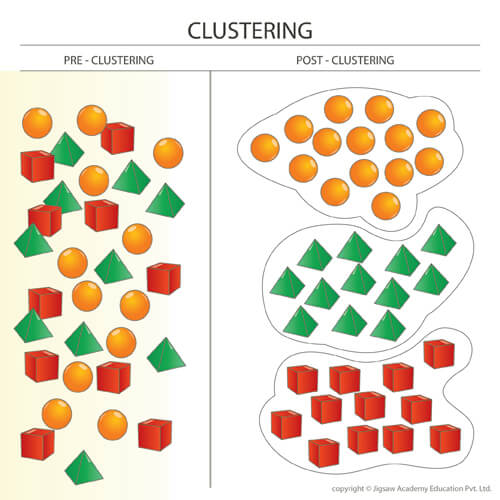
\includegraphics{images/cluster1.jpg}
\caption{\label{fig:cluster1}Przykład nienadzorowanego uczenia maszynowego.~ \emph{Źródło:}\url{https://analyticstraining.com/cluster-analysis-for-business/}}
\end{figure}

href=``\url{https://twitter.com/i/status/1097199751072690176}''\textgreater{}Ferbruary 17, 2019

\hypertarget{etapy-eksploracji-danych}{%
\section*{Etapy eksploracji danych}\label{etapy-eksploracji-danych}}
\addcontentsline{toc}{section}{Etapy eksploracji danych}

\begin{figure}
\centering
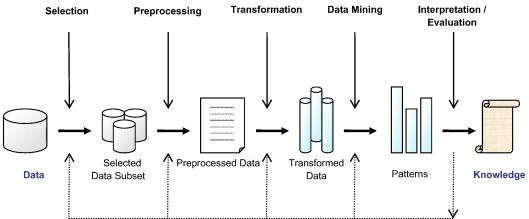
\includegraphics{images/dm_stages.jpg}
\caption{\label{fig:unnamed-chunk-2}Etapy eksploracji danych (Kavakiotis et al. \protect\hyperlink{ref-kavakiotis2017}{2017})}
\end{figure}

\begin{enumerate}
\def\labelenumi{\arabic{enumi}.}
\tightlist
\item
  Czyszczenie danych - polega na usuwaniu braków danych, usuwaniu stałych zmiennych, imputacji braków danych oraz przygotowaniu danych do dalszych analiz.
\item
  Integracja danych - łączenie danych pochodzących z różnych źródeł.
\item
  Selekcja danych - wybór z bazy tych danych, które są potrzebne do dalszych analiz.
\item
  Transformacja danych - przekształcenie i konsolidacja danych do postaci przydatnej do eksploracji.
\item
  Eksploracja danych - zastosowanie technik wymienionych wcześniej w celu odnalezienia wzorców\footnote{ang. \emph{patterns}} i zależności.
\item
  Ewaluacja modeli - ocena poprawności modeli oraz wzorców z nich uzyskanych.
\item
  Wizualizacja wyników - graficzne przedstawienie odkrytych wzorców.
\item
  Wdrażanie modeli - zastosowanie wyznaczonych wzorców.
\end{enumerate}

\hypertarget{roz1}{%
\chapter{Import danych}\label{roz1}}

Środowisko \textbf{R} pozwala na import i export plików o różnych rozszerzeniach (\texttt{txt,\ csv,\ xls,\ xlsx,\ sav,\ xpt,\ dta}, itd.)\footnote{póki co nie jest mi znana funkcja pozwalająca na import plików programu Statistica}. W tym celu czasami trzeba zainstalować pakiety rozszerzające podstawowe możliwości R-a. Najnowsza\footnote{na dzień 19.02.2019} wersja programu \href{https://www.rstudio.com}{RStudio} (v. 1.1.463)\footnote{istnieją rownież nowsze wersje deweloperskie} pozwala na wczytanie danych z popularnych źródeł za pomocą GUI.

\begin{figure}
\centering
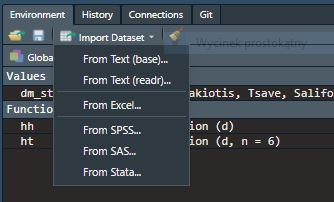
\includegraphics{images/import.JPG}
\caption{\label{fig:import1}Narzędzie do importu plików programu RStudio}
\end{figure}

Jeśli dane są zapisane w trybie tekstowym (np. \texttt{txt}, \texttt{csv}), to wczytujemy je w następujący sposób

\begin{Shaded}
\begin{Highlighting}[]
\NormalTok{dane1 <-}\StringTok{ }\KeywordTok{read.table}\NormalTok{(}\StringTok{"data/dane1.txt"}\NormalTok{, }\DataTypeTok{header =}\NormalTok{ T)}
\KeywordTok{head}\NormalTok{(dane1)}
\end{Highlighting}
\end{Shaded}

\begin{verbatim}
##   Sepal.Length Sepal.Width Petal.Length Petal.Width Species
## 1          5.1         3.5          1.4         0.2  setosa
## 2          4.9         3.0          1.4         0.2  setosa
## 3          4.7         3.2          1.3         0.2  setosa
## 4          4.6         3.1          1.5         0.2  setosa
## 5          5.0         3.6          1.4         0.2  setosa
## 6          5.4         3.9          1.7         0.4  setosa
\end{verbatim}

\begin{Shaded}
\begin{Highlighting}[]
\NormalTok{dane2 <-}\StringTok{ }\KeywordTok{read.csv2}\NormalTok{(}\StringTok{"data/dane1.csv"}\NormalTok{, }\DataTypeTok{header =}\NormalTok{ T)}
\KeywordTok{head}\NormalTok{(dane2)}
\end{Highlighting}
\end{Shaded}

\begin{verbatim}
##   Sepal.Length Sepal.Width Petal.Length Petal.Width Species
## 1          5.1         3.5          1.4         0.2  setosa
## 2          4.9         3.0          1.4         0.2  setosa
## 3          4.7         3.2          1.3         0.2  setosa
## 4          4.6         3.1          1.5         0.2  setosa
## 5          5.0         3.6          1.4         0.2  setosa
## 6          5.4         3.9          1.7         0.4  setosa
\end{verbatim}

\begin{Shaded}
\begin{Highlighting}[]
\CommentTok{# funkcja pakietu readr wczytuje plik jako ramkę danych w formacie tibble}
\CommentTok{# pakiet readr jest częsią większego pakietu tidyverse, }
\CommentTok{# który został wczytany wczsniej}
\NormalTok{dane3 <-}\StringTok{ }\KeywordTok{read_csv2}\NormalTok{(}\StringTok{"data/dane1.csv"}\NormalTok{)}
\NormalTok{dane3}
\end{Highlighting}
\end{Shaded}

\begin{verbatim}
## # A tibble: 150 x 5
##    Sepal.Length Sepal.Width Petal.Length Petal.Width Species
##           <dbl>       <dbl>        <dbl>       <dbl> <chr>  
##  1          5.1         3.5          1.4         0.2 setosa 
##  2          4.9         3            1.4         0.2 setosa 
##  3          4.7         3.2          1.3         0.2 setosa 
##  4          4.6         3.1          1.5         0.2 setosa 
##  5          5           3.6          1.4         0.2 setosa 
##  6          5.4         3.9          1.7         0.4 setosa 
##  7          4.6         3.4          1.4         0.3 setosa 
##  8          5           3.4          1.5         0.2 setosa 
##  9          4.4         2.9          1.4         0.2 setosa 
## 10          4.9         3.1          1.5         0.1 setosa 
## # ... with 140 more rows
\end{verbatim}

Jeśli dane są przechowywane w pliku Excel (np. \texttt{xlsx}), to importujemy je za pomocą funkcji \texttt{read\_excel} pakietu \texttt{readxl}. Domyślnie jest wczytywany arkusz pierwszy ale jeśli zachodzi taka potrzeba, to można ustalić, który arkusz pliku Excel ma być wczytany za pomocą paramteru \texttt{sheet}, np. \texttt{sheet=3}, co oznacza, że zostanie wczytany trzeci arkusz pliku.

\begin{figure}
\centering
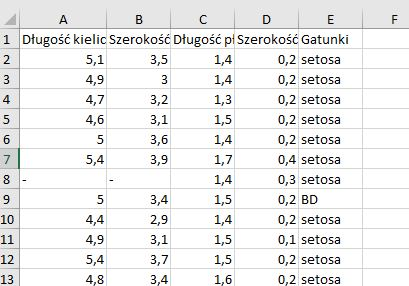
\includegraphics{images/excel.jpg}
\caption{\label{fig:excel}Fragment pliku Excel}
\end{figure}

Ponieważ w pliku \texttt{dane1.xlsx} braki danych zostały zakodowane znakami \texttt{BD} oraz \texttt{-}, to należy ten fakt przekazać funkcji, aby poprawnie wczytać braki danych. W przeciwnym przypadku zmienne zawierające braki tak kodowane, będą wczytane jako zmienne znakowe.

\begin{Shaded}
\begin{Highlighting}[]
\KeywordTok{library}\NormalTok{(readxl)}
\NormalTok{dane4 <-}\StringTok{ }\KeywordTok{read_excel}\NormalTok{(}\StringTok{"data/dane1.xlsx"}\NormalTok{, }\DataTypeTok{na =} \KeywordTok{c}\NormalTok{(}\StringTok{"BD"}\NormalTok{, }\StringTok{"-"}\NormalTok{))}
\NormalTok{dane4}
\end{Highlighting}
\end{Shaded}

\begin{verbatim}
## # A tibble: 150 x 5
##    `Długość kielic~ `Szerokość kiel~ `Długość płatka` `Szerokość płat~
##               <dbl>            <dbl>            <dbl>            <dbl>
##  1              5.1              3.5              1.4              0.2
##  2              4.9              3                1.4              0.2
##  3              4.7              3.2              1.3              0.2
##  4              4.6              3.1              1.5              0.2
##  5              5                3.6              1.4              0.2
##  6              5.4              3.9              1.7              0.4
##  7             NA               NA                1.4              0.3
##  8              5                3.4              1.5              0.2
##  9              4.4              2.9              1.4              0.2
## 10              4.9              3.1              1.5              0.1
## # ... with 140 more rows, and 1 more variable: Gatunki <chr>
\end{verbatim}

Istniej oczywiście jeszcze wiele innych fomatów danych, charakterystycznych dla programów, w których są traktowane jako domyślne.\footnote{do ich wczytywania stosujemy funkcje pakietu \texttt{foreign}} W szczególny sposób należy zwrócić uwagę na pliki o rozszerzeniu \texttt{RData} lub \texttt{rda}\footnote{oznaczają to samo} oraz pliki \texttt{rds}. Pliki \texttt{rda} służą do przechowywania obiektów programu \texttt{R}. Mogą to być pliki danych ale również obiekty graficzne (typu wyniki funkcji \texttt{ggplot}), modele (np. wynik funkcji \texttt{lm()}), zdefiniowane funkcje i wszystkie inne obiekty, które da się zapisać w środowisku \texttt{R}. Ponadto pliki \texttt{rda} pozawalają na zapisanie wielu obiektów w jednym pliku. Pliki o rozszerzeniu \texttt{rds} mają podobną funkcję z tym, że pozwalają na przechowywanie tylko jednego obiektu.

\begin{Shaded}
\begin{Highlighting}[]
\CommentTok{# wszystkie wczytane wcześniej pliki zapisuje w jednym pliku}
\KeywordTok{save}\NormalTok{(dane1, dane2, dane3, dane4, }\DataTypeTok{file =} \StringTok{"data/dane.rda"}\NormalTok{)}
\CommentTok{# plik rda został zapisany}
\KeywordTok{list.files}\NormalTok{(}\DataTypeTok{path =} \StringTok{"data/"}\NormalTok{)}
\end{Highlighting}
\end{Shaded}

\begin{verbatim}
## [1] "algae.csv"    "Analysis.txt" "dane.rda"     "dane1.csv"   
## [5] "dane1.txt"    "dane1.xlsx"   "dane4.rds"    "dane4.sav"
\end{verbatim}

\begin{Shaded}
\begin{Highlighting}[]
\CommentTok{# usuwam dane ze środowiska R}
\KeywordTok{rm}\NormalTok{(dane1, dane2, dane3, dane4)}
\CommentTok{# sprawdzam co jest wczytane do R}
\KeywordTok{ls}\NormalTok{()}
\end{Highlighting}
\end{Shaded}

\begin{verbatim}
## character(0)
\end{verbatim}

\begin{Shaded}
\begin{Highlighting}[]
\CommentTok{# wczytuję plik rda}
\KeywordTok{load}\NormalTok{(}\StringTok{"data/dane.rda"}\NormalTok{)}
\CommentTok{# jeszcze raz sprawdzam co jest wczytane do R}
\KeywordTok{ls}\NormalTok{()}
\end{Highlighting}
\end{Shaded}

\begin{verbatim}
## [1] "dane1" "dane2" "dane3" "dane4"
\end{verbatim}

Zapisując obiekty jako oddzielne pliki, można przy wczytywaniu nadawać im nazwy.

\begin{Shaded}
\begin{Highlighting}[]
\KeywordTok{rm}\NormalTok{(dane1, dane2, dane3)}
\KeywordTok{ls}\NormalTok{()}
\end{Highlighting}
\end{Shaded}

\begin{verbatim}
## [1] "dane4"
\end{verbatim}

\begin{Shaded}
\begin{Highlighting}[]
\KeywordTok{saveRDS}\NormalTok{(dane4, }\DataTypeTok{file =} \StringTok{"data/dane4.rds"}\NormalTok{)}
\NormalTok{nowe_dane <-}\StringTok{ }\KeywordTok{readRDS}\NormalTok{(}\StringTok{"data/dane4.rds"}\NormalTok{)}
\NormalTok{nowe_dane}
\end{Highlighting}
\end{Shaded}

\begin{verbatim}
## # A tibble: 150 x 5
##    `Długość kielic~ `Szerokość kiel~ `Długość płatka` `Szerokość płat~
##               <dbl>            <dbl>            <dbl>            <dbl>
##  1              5.1              3.5              1.4              0.2
##  2              4.9              3                1.4              0.2
##  3              4.7              3.2              1.3              0.2
##  4              4.6              3.1              1.5              0.2
##  5              5                3.6              1.4              0.2
##  6              5.4              3.9              1.7              0.4
##  7             NA               NA                1.4              0.3
##  8              5                3.4              1.5              0.2
##  9              4.4              2.9              1.4              0.2
## 10              4.9              3.1              1.5              0.1
## # ... with 140 more rows, and 1 more variable: Gatunki <chr>
\end{verbatim}

Oprócz wielu zalet takiego sposobu importu i eksportu danych jest jedna poważna wada, pliki te można odczytać jedynie za pomocą \texttt{R}. Osobiście polecam stosować do importu i eksportu danych plików w takich formatach, które mogą przeczytać wszyscy. Jak dotąd widać do importu różnych formatów danych potrzebujemy różnych funkcji, czasami nawet z różnych pakietów. Istnieje rozwiązanie tej niedogodności 😆

\begin{Shaded}
\begin{Highlighting}[]
\KeywordTok{library}\NormalTok{(rio)}
\NormalTok{dane1 <-}\StringTok{ }\KeywordTok{import}\NormalTok{(}\StringTok{"data/dane1.txt"}\NormalTok{)}
\KeywordTok{head}\NormalTok{(dane1)}
\end{Highlighting}
\end{Shaded}

\begin{verbatim}
##   Sepal.Length Sepal.Width Petal.Length Petal.Width Species
## 1          5.1         3.5          1.4         0.2  setosa
## 2          4.9         3.0          1.4         0.2  setosa
## 3          4.7         3.2          1.3         0.2  setosa
## 4          4.6         3.1          1.5         0.2  setosa
## 5          5.0         3.6          1.4         0.2  setosa
## 6          5.4         3.9          1.7         0.4  setosa
\end{verbatim}

\begin{Shaded}
\begin{Highlighting}[]
\NormalTok{dane2 <-}\StringTok{ }\KeywordTok{import}\NormalTok{(}\StringTok{"data/dane1.csv"}\NormalTok{, }\DataTypeTok{dec =} \StringTok{","}\NormalTok{)}
\CommentTok{# dane1.csv miały , jako znak rozdzielający cechę i mantysę liczb}
\CommentTok{# dlatego włączamy parametr dec}
\KeywordTok{head}\NormalTok{(dane2)}
\end{Highlighting}
\end{Shaded}

\begin{verbatim}
##   Sepal.Length Sepal.Width Petal.Length Petal.Width Species
## 1          5.1         3.5          1.4         0.2  setosa
## 2          4.9         3.0          1.4         0.2  setosa
## 3          4.7         3.2          1.3         0.2  setosa
## 4          4.6         3.1          1.5         0.2  setosa
## 5          5.0         3.6          1.4         0.2  setosa
## 6          5.4         3.9          1.7         0.4  setosa
\end{verbatim}

\begin{Shaded}
\begin{Highlighting}[]
\NormalTok{dane3 <-}\StringTok{ }\KeywordTok{import}\NormalTok{(}\StringTok{"data/dane1.xlsx"}\NormalTok{, }\DataTypeTok{na=}\KeywordTok{c}\NormalTok{(}\StringTok{"BD"}\NormalTok{,}\StringTok{"-"}\NormalTok{))}
\KeywordTok{head}\NormalTok{(dane3)}
\end{Highlighting}
\end{Shaded}

\begin{verbatim}
##   Długość kielicha Szerokość kielicha Długość płatka Szerokość płatka
## 1              5.1                3.5            1.4              0.2
## 2              4.9                3.0            1.4              0.2
## 3              4.7                3.2            1.3              0.2
## 4              4.6                3.1            1.5              0.2
## 5              5.0                3.6            1.4              0.2
## 6              5.4                3.9            1.7              0.4
##   Gatunki
## 1  setosa
## 2  setosa
## 3  setosa
## 4  setosa
## 5  setosa
## 6  setosa
\end{verbatim}

\begin{Shaded}
\begin{Highlighting}[]
\NormalTok{dane4 <-}\StringTok{ }\KeywordTok{import}\NormalTok{(}\StringTok{"data/dane4.rds"}\NormalTok{)}
\NormalTok{dane4}
\end{Highlighting}
\end{Shaded}

\begin{verbatim}
## # A tibble: 150 x 5
##    `Długość kielic~ `Szerokość kiel~ `Długość płatka` `Szerokość płat~
##               <dbl>            <dbl>            <dbl>            <dbl>
##  1              5.1              3.5              1.4              0.2
##  2              4.9              3                1.4              0.2
##  3              4.7              3.2              1.3              0.2
##  4              4.6              3.1              1.5              0.2
##  5              5                3.6              1.4              0.2
##  6              5.4              3.9              1.7              0.4
##  7             NA               NA                1.4              0.3
##  8              5                3.4              1.5              0.2
##  9              4.4              2.9              1.4              0.2
## 10              4.9              3.1              1.5              0.1
## # ... with 140 more rows, and 1 more variable: Gatunki <chr>
\end{verbatim}

Lista możliwości jaką daje nam pakiet \texttt{rio} (Chan and Leeper \protect\hyperlink{ref-R-rio}{2018}) jest niemal nieograniczona:\footnote{fragment pliku \texttt{help} funkcji \texttt{import}}

\begin{itemize}
\tightlist
\item
  Comma-separated data (.csv), using fread or, if fread = FALSE, read.table with row.names = FALSE and stringsAsFactors = FALSE
\item
  Pipe-separated data (.psv), using fread or, if fread = FALSE, read.table with sep = `\textbar{}', row.names = FALSE and stringsAsFactors = FALSE
\item
  Tab-separated data (.tsv), using fread or, if fread = FALSE, read.table with row.names = FALSE and stringsAsFactors = FALSE
\item
  SAS (.sas7bdat), using read\_sas.
\item
  SAS XPORT (.xpt), using read\_xpt or, if haven = FALSE, read.xport.
\item
  SPSS (.sav), using read\_sav. If haven = FALSE, read.spss can be used.
\item
  Stata (.dta), using read\_dta. If haven = FALSE, read.dta can be used.
\item
  SAS XPORT (.xpt), using read.xport.
\item
  SPSS Portable Files (.por), using read\_por.
\item
  Excel (.xls and .xlsx), using read\_excel. Use which to specify a sheet number. For .xlsx files, it is possible to set readxl = FALSE, so that read.xlsx can be used instead of readxl (the default).
\item
  R syntax object (.R), using dget
\item
  Saved R objects (.RData,.rda), using load for single-object .Rdata files. Use which to specify an object name for multi-object .Rdata files. This can be any R object (not just a data frame).
\item
  Serialized R objects (.rds), using readRDS. This can be any R object (not just a data frame).
\item
  Epiinfo (.rec), using read.epiinfo
\item
  Minitab (.mtp), using read.mtp
\item
  Systat (.syd), using read.systat
\item
  ``XBASE'' database files (.dbf), using read.dbf
\item
  Weka Attribute-Relation File Format (.arff), using read.arff
\item
  Data Interchange Format (.dif), using read.DIF
\item
  Fortran data (no recognized extension), using read.fortran
\item
  Fixed-width format data (.fwf), using a faster version of read.fwf that requires a widths argument and by default in rio has stringsAsFactors = FALSE. If readr = TRUE, import will be performed using read\_fwf, where widths should be: NULL, a vector of column widths, or the output of fwf\_empty, fwf\_widths, or fwf\_positions.
\item
  gzip comma-separated data (.csv.gz), using read.table with row.names = FALSE and stringsAsFactors = FALSE
\item
  CSVY (CSV with a YAML metadata header) using read\_csvy.
\item
  Feather R/Python interchange format (.feather), using read\_feather
\item
  Fast storage (.fst), using read.fst
\item
  JSON (.json), using fromJSON
\item
  Matlab (.mat), using read.mat
\item
  EViews (.wf1), using readEViews
\item
  OpenDocument Spreadsheet (.ods), using read\_ods. Use which to specify a sheet number.
\item
  Single-table HTML documents (.html), using read\_html. The data structure will only be read correctly if the HTML file can be converted to a list via as\_list.
\item
  Shallow XML documents (.xml), using read\_xml. The data structure will only be read correctly if the XML file can be converted to a list via as\_list.
\item
  YAML (.yml), using yaml.load
\item
  Clipboard import (on Windows and Mac OS), using read.table with row.names = FALSE
\item
  Google Sheets, as Comma-separated data (.csv)
\end{itemize}

\BeginKnitrBlock{example}
\protect\hypertarget{exm:przyk1}{}{\label{exm:przyk1} }Poniższa ilustracja przedstawia fragment pliku danych \texttt{Analysis.txt} zawierającego pewne błędy, które należy naprawić na etapie importu danych. Po pierwsze brakuje w nim nazw zmiennych (choć nie widać tego na rysunku). Poszczególne kolumny nazywają się następująco: \texttt{season}, \texttt{size}, \texttt{speed}, \texttt{mxPH}, \texttt{mnO2}, \texttt{Cl}, \texttt{NO3}, \texttt{NH4}, \texttt{oPO4}, \texttt{PO4}, \texttt{Chla}, \texttt{a1}, \texttt{a2}, \texttt{a3}, \texttt{a4}, \texttt{a5}, \texttt{a6}, \texttt{a7}. Naszym zadaniem jest import tego pliku z jednoczesną obsługą braków (braki danych są zakodowane przez \texttt{XXXXXXX}) oraz nadaniem nagłówków kolumn. Plik \texttt{Analisis.txt} jest umieszczony w kagalogu \texttt{data/}. Z racji, że plik dotyczy glonów, to dane zapiszemy pod nazwą \texttt{algae}.
\EndKnitrBlock{example}

\begin{figure}
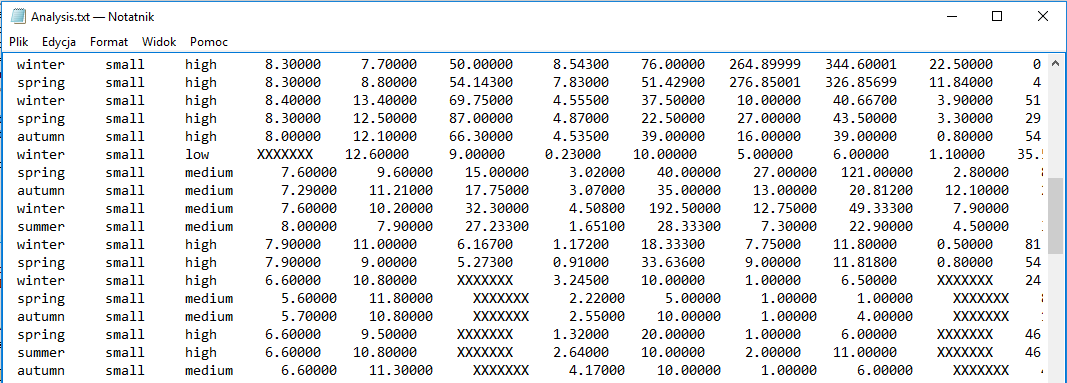
\includegraphics[width=10.67in]{images/analalysi_foto} \caption{Fragment pliku danych Analisis.txt}\label{fig:foto}
\end{figure}

\begin{Shaded}
\begin{Highlighting}[]
\NormalTok{algae <-}\StringTok{ }\KeywordTok{import}\NormalTok{(}\StringTok{'data/Analysis.txt'}\NormalTok{, }\DataTypeTok{header=}\NormalTok{F, }
                \DataTypeTok{dec=}\StringTok{'.'}\NormalTok{, }
                \DataTypeTok{col.names=}\KeywordTok{c}\NormalTok{(}\StringTok{'season'}\NormalTok{,}\StringTok{'size'}\NormalTok{,}\StringTok{'speed'}\NormalTok{,}\StringTok{'mxPH'}\NormalTok{,}\StringTok{'mnO2'}\NormalTok{,}\StringTok{'Cl'}\NormalTok{,}
                            \StringTok{'NO3'}\NormalTok{,}\StringTok{'NH4'}\NormalTok{,}\StringTok{'oPO4'}\NormalTok{,}\StringTok{'PO4'}\NormalTok{,}\StringTok{'Chla'}\NormalTok{,}\StringTok{'a1'}\NormalTok{,}\StringTok{'a2'}\NormalTok{,}
                            \StringTok{'a3'}\NormalTok{,}\StringTok{'a4'}\NormalTok{,}\StringTok{'a5'}\NormalTok{,}\StringTok{'a6'}\NormalTok{,}\StringTok{'a7'}\NormalTok{),}
                \DataTypeTok{na.strings=}\KeywordTok{c}\NormalTok{(}\StringTok{'XXXXXXX'}\NormalTok{))}
\KeywordTok{head}\NormalTok{(algae)}
\end{Highlighting}
\end{Shaded}

\begin{verbatim}
##   season  size  speed mxPH mnO2     Cl    NO3     NH4    oPO4     PO4 Chla
## 1 winter small medium 8.00  9.8 60.800  6.238 578.000 105.000 170.000 50.0
## 2 spring small medium 8.35  8.0 57.750  1.288 370.000 428.750 558.750  1.3
## 3 autumn small medium 8.10 11.4 40.020  5.330 346.667 125.667 187.057 15.6
## 4 spring small medium 8.07  4.8 77.364  2.302  98.182  61.182 138.700  1.4
## 5 autumn small medium 8.06  9.0 55.350 10.416 233.700  58.222  97.580 10.5
## 6 winter small   high 8.25 13.1 65.750  9.248 430.000  18.250  56.667 28.4
##     a1   a2   a3  a4   a5   a6  a7
## 1  0.0  0.0  0.0 0.0 34.2  8.3 0.0
## 2  1.4  7.6  4.8 1.9  6.7  0.0 2.1
## 3  3.3 53.6  1.9 0.0  0.0  0.0 9.7
## 4  3.1 41.0 18.9 0.0  1.4  0.0 1.4
## 5  9.2  2.9  7.5 0.0  7.5  4.1 1.0
## 6 15.1 14.6  1.4 0.0 22.5 12.6 2.9
\end{verbatim}

\begin{Shaded}
\begin{Highlighting}[]
\KeywordTok{summary}\NormalTok{(algae)}
\end{Highlighting}
\end{Shaded}

\begin{verbatim}
##     season              size              speed                mxPH      
##  Length:200         Length:200         Length:200         Min.   :5.600  
##  Class :character   Class :character   Class :character   1st Qu.:7.700  
##  Mode  :character   Mode  :character   Mode  :character   Median :8.060  
##                                                           Mean   :8.012  
##                                                           3rd Qu.:8.400  
##                                                           Max.   :9.700  
##                                                           NA's   :1      
##       mnO2              Cl               NO3              NH4          
##  Min.   : 1.500   Min.   :  0.222   Min.   : 0.050   Min.   :    5.00  
##  1st Qu.: 7.725   1st Qu.: 10.981   1st Qu.: 1.296   1st Qu.:   38.33  
##  Median : 9.800   Median : 32.730   Median : 2.675   Median :  103.17  
##  Mean   : 9.118   Mean   : 43.636   Mean   : 3.282   Mean   :  501.30  
##  3rd Qu.:10.800   3rd Qu.: 57.824   3rd Qu.: 4.446   3rd Qu.:  226.95  
##  Max.   :13.400   Max.   :391.500   Max.   :45.650   Max.   :24064.00  
##  NA's   :2        NA's   :10        NA's   :2        NA's   :2         
##       oPO4             PO4              Chla               a1       
##  Min.   :  1.00   Min.   :  1.00   Min.   :  0.200   Min.   : 0.00  
##  1st Qu.: 15.70   1st Qu.: 41.38   1st Qu.:  2.000   1st Qu.: 1.50  
##  Median : 40.15   Median :103.29   Median :  5.475   Median : 6.95  
##  Mean   : 73.59   Mean   :137.88   Mean   : 13.971   Mean   :16.92  
##  3rd Qu.: 99.33   3rd Qu.:213.75   3rd Qu.: 18.308   3rd Qu.:24.80  
##  Max.   :564.60   Max.   :771.60   Max.   :110.456   Max.   :89.80  
##  NA's   :2        NA's   :2        NA's   :12                       
##        a2               a3               a4               a5        
##  Min.   : 0.000   Min.   : 0.000   Min.   : 0.000   Min.   : 0.000  
##  1st Qu.: 0.000   1st Qu.: 0.000   1st Qu.: 0.000   1st Qu.: 0.000  
##  Median : 3.000   Median : 1.550   Median : 0.000   Median : 1.900  
##  Mean   : 7.458   Mean   : 4.309   Mean   : 1.992   Mean   : 5.064  
##  3rd Qu.:11.375   3rd Qu.: 4.925   3rd Qu.: 2.400   3rd Qu.: 7.500  
##  Max.   :72.600   Max.   :42.800   Max.   :44.600   Max.   :44.400  
##                                                                     
##        a6               a7        
##  Min.   : 0.000   Min.   : 0.000  
##  1st Qu.: 0.000   1st Qu.: 0.000  
##  Median : 0.000   Median : 1.000  
##  Mean   : 5.964   Mean   : 2.495  
##  3rd Qu.: 6.925   3rd Qu.: 2.400  
##  Max.   :77.600   Max.   :31.600  
## 
\end{verbatim}

\begin{Shaded}
\begin{Highlighting}[]
\KeywordTok{export}\NormalTok{(algae, }\DataTypeTok{file =} \StringTok{"data/algae.csv"}\NormalTok{)}
\end{Highlighting}
\end{Shaded}

\hypertarget{przygotowanie-danych}{%
\chapter{Przygotowanie danych}\label{przygotowanie-danych}}

Dane, które importujemy z zewnętrznego źródła najczęściej nie spełniają formatów obowiązujących w \textbf{R}. Często zmienne zawierają niedopuszczalne znaki szczególne, odstępy w nazwach, powtórzone nazwy kolumn, nazwy zmiennych zaczynające się od liczby, czy puste wiersze lub kolumny. Przed przystąpieniem do analizy zbioru należy rozważyć ewentualne poprawki nazw zmiennych, czy usunięcie pustych kolumn i wierszy. Niektórych czynności można dokonać już na etapie importu danych, stosując pewne pakiety oraz nowe funkcjonalności środowiska \textbf{RStudio}. W większości przypadków uchroni nas to od żmudnego przekształcania typów zmiennych. Oczywiście wszystkie te czynności czyszczenia danych można również dokonać już po imporcie danych, za pomocą odpowiednich komend \textbf{R}.

\begin{Shaded}
\begin{Highlighting}[]
\CommentTok{## przykładowe niepożądane nazwy zmiennych}
\NormalTok{test_df <-}\StringTok{ }\KeywordTok{as.data.frame}\NormalTok{(}\KeywordTok{matrix}\NormalTok{(}\KeywordTok{rnorm}\NormalTok{(}\DecValTok{18}\NormalTok{),}\DataTypeTok{ncol =} \DecValTok{6}\NormalTok{))}
\KeywordTok{names}\NormalTok{(test_df) <-}\StringTok{ }\KeywordTok{c}\NormalTok{(}\StringTok{"hIgHlo"}\NormalTok{, }\StringTok{"REPEAT VALUE"}\NormalTok{, }\StringTok{"REPEAT VALUE"}\NormalTok{,}
                    \StringTok{"% successful (2009)"}\NormalTok{,  }\StringTok{"abc@!*"}\NormalTok{, }\StringTok{""}\NormalTok{)}
\NormalTok{test_df}
\end{Highlighting}
\end{Shaded}

\begin{verbatim}
##        hIgHlo REPEAT VALUE REPEAT VALUE % successful (2009)      abc@!*
## 1  0.62816036   -0.5201609    1.1043470           0.1738823 -0.08412172
## 2 -0.28213680   -0.6262217   -0.1659695           1.2445501  1.15968770
## 3  0.09870219   -0.6941247   -0.4375282           0.1012135  1.02700292
##             
## 1  2.3730675
## 2  0.4643571
## 3 -0.6335834
\end{verbatim}

\begin{Shaded}
\begin{Highlighting}[]
\CommentTok{## do poprawy nazw zmiennych użyjemy funkcji make.names}
\KeywordTok{names}\NormalTok{(test_df) <-}\StringTok{ }\KeywordTok{make.names}\NormalTok{(}\KeywordTok{names}\NormalTok{(test_df))}
\NormalTok{test_df}
\end{Highlighting}
\end{Shaded}

\begin{verbatim}
##        hIgHlo REPEAT.VALUE REPEAT.VALUE X..successful..2009.      abc...
## 1  0.62816036   -0.5201609    1.1043470            0.1738823 -0.08412172
## 2 -0.28213680   -0.6262217   -0.1659695            1.2445501  1.15968770
## 3  0.09870219   -0.6941247   -0.4375282            0.1012135  1.02700292
##            X
## 1  2.3730675
## 2  0.4643571
## 3 -0.6335834
\end{verbatim}

Efekt końcowy choć skuteczny, to nie jest zadowalający. Czyszczenia nazw zmiennych można też dokonać stosując funkcję \texttt{clean\_names} pakietu \textbf{janitor} (Firke \protect\hyperlink{ref-R-janitor}{2018}). Pozwala on również na usuwanie pustych wierszy i kolumn, znajdowanie zduplikowanych rekordów, itp.

\begin{Shaded}
\begin{Highlighting}[]
\KeywordTok{library}\NormalTok{(janitor)}
\NormalTok{test_df }\OperatorTok\StringTok{ }\CommentTok{# aby na stałe zmienić nazwy zmiennych trzeba podstawienia}
\StringTok{    }\KeywordTok{clean_names}\NormalTok{()}
\end{Highlighting}
\end{Shaded}

\begin{verbatim}
##      h_ig_hlo repeat_value repeat_value_2 x_successful_2009         abc
## 1  0.62816036   -0.5201609      1.1043470         0.1738823 -0.08412172
## 2 -0.28213680   -0.6262217     -0.1659695         1.2445501  1.15968770
## 3  0.09870219   -0.6941247     -0.4375282         0.1012135  1.02700292
##            x
## 1  2.3730675
## 2  0.4643571
## 3 -0.6335834
\end{verbatim}

\begin{Shaded}
\begin{Highlighting}[]
\CommentTok{# przykładowe dane}
\NormalTok{x <-}\StringTok{ }\KeywordTok{data.frame}\NormalTok{(}\DataTypeTok{w1=}\KeywordTok{c}\NormalTok{(}\DecValTok{1}\NormalTok{,}\DecValTok{4}\NormalTok{,}\DecValTok{2}\NormalTok{,}\OtherTok{NA}\NormalTok{),}\DataTypeTok{w2=}\KeywordTok{c}\NormalTok{(}\OtherTok{NA}\NormalTok{,}\DecValTok{2}\NormalTok{,}\DecValTok{3}\NormalTok{,}\OtherTok{NA}\NormalTok{), }\DataTypeTok{w3=}\KeywordTok{c}\NormalTok{(}\DecValTok{1}\NormalTok{,}\OtherTok{NA}\NormalTok{,}\DecValTok{1}\NormalTok{,}\OtherTok{NA}\NormalTok{))}
\NormalTok{x}
\end{Highlighting}
\end{Shaded}

\begin{verbatim}
##   w1 w2 w3
## 1  1 NA  1
## 2  4  2 NA
## 3  2  3  1
## 4 NA NA NA
\end{verbatim}

\begin{Shaded}
\begin{Highlighting}[]
\NormalTok{x }\OperatorTok\StringTok{ }\KeywordTok{remove_empty}\NormalTok{(}\StringTok{"rows"}\NormalTok{)}
\end{Highlighting}
\end{Shaded}

\begin{verbatim}
##   w1 w2 w3
## 1  1 NA  1
## 2  4  2 NA
## 3  2  3  1
\end{verbatim}

\hypertarget{identyfikacja-brakow-danych}{%
\section{Identyfikacja braków danych}\label{identyfikacja-brakow-danych}}

Zanim usuniemy jakiekolwiek braki w zbiorze, powinniśmy je najpierw zidentyfikować, określić ich charakter, a dopiero potem ewentualnie podjąć decyzję o uzupełnianiu braków.

\begin{Shaded}
\begin{Highlighting}[]
\NormalTok{algae <-}\StringTok{ }\NormalTok{rio}\OperatorTok{::}\KeywordTok{import}\NormalTok{(}\StringTok{"data/algae.csv"}\NormalTok{)}

\CommentTok{# najprościej jest wywołać summary}
\KeywordTok{summary}\NormalTok{(algae)}
\end{Highlighting}
\end{Shaded}

\begin{verbatim}
##     season              size              speed                mxPH      
##  Length:200         Length:200         Length:200         Min.   :5.600  
##  Class :character   Class :character   Class :character   1st Qu.:7.700  
##  Mode  :character   Mode  :character   Mode  :character   Median :8.060  
##                                                           Mean   :8.012  
##                                                           3rd Qu.:8.400  
##                                                           Max.   :9.700  
##                                                           NA's   :1      
##       mnO2              Cl               NO3              NH4          
##  Min.   : 1.500   Min.   :  0.222   Min.   : 0.050   Min.   :    5.00  
##  1st Qu.: 7.725   1st Qu.: 10.981   1st Qu.: 1.296   1st Qu.:   38.33  
##  Median : 9.800   Median : 32.730   Median : 2.675   Median :  103.17  
##  Mean   : 9.118   Mean   : 43.636   Mean   : 3.282   Mean   :  501.30  
##  3rd Qu.:10.800   3rd Qu.: 57.824   3rd Qu.: 4.446   3rd Qu.:  226.95  
##  Max.   :13.400   Max.   :391.500   Max.   :45.650   Max.   :24064.00  
##  NA's   :2        NA's   :10        NA's   :2        NA's   :2         
##       oPO4             PO4              Chla               a1       
##  Min.   :  1.00   Min.   :  1.00   Min.   :  0.200   Min.   : 0.00  
##  1st Qu.: 15.70   1st Qu.: 41.38   1st Qu.:  2.000   1st Qu.: 1.50  
##  Median : 40.15   Median :103.29   Median :  5.475   Median : 6.95  
##  Mean   : 73.59   Mean   :137.88   Mean   : 13.971   Mean   :16.92  
##  3rd Qu.: 99.33   3rd Qu.:213.75   3rd Qu.: 18.308   3rd Qu.:24.80  
##  Max.   :564.60   Max.   :771.60   Max.   :110.456   Max.   :89.80  
##  NA's   :2        NA's   :2        NA's   :12                       
##        a2               a3               a4               a5        
##  Min.   : 0.000   Min.   : 0.000   Min.   : 0.000   Min.   : 0.000  
##  1st Qu.: 0.000   1st Qu.: 0.000   1st Qu.: 0.000   1st Qu.: 0.000  
##  Median : 3.000   Median : 1.550   Median : 0.000   Median : 1.900  
##  Mean   : 7.458   Mean   : 4.309   Mean   : 1.992   Mean   : 5.064  
##  3rd Qu.:11.375   3rd Qu.: 4.925   3rd Qu.: 2.400   3rd Qu.: 7.500  
##  Max.   :72.600   Max.   :42.800   Max.   :44.600   Max.   :44.400  
##                                                                     
##        a6               a7        
##  Min.   : 0.000   Min.   : 0.000  
##  1st Qu.: 0.000   1st Qu.: 0.000  
##  Median : 0.000   Median : 1.000  
##  Mean   : 5.964   Mean   : 2.495  
##  3rd Qu.: 6.925   3rd Qu.: 2.400  
##  Max.   :77.600   Max.   :31.600  
## 
\end{verbatim}

\begin{Shaded}
\begin{Highlighting}[]
\CommentTok{## wyświetl niekompletne wiersze}
\NormalTok{algae[}\OperatorTok{!}\KeywordTok{complete.cases}\NormalTok{(algae),] }\OperatorTok\StringTok{ }\KeywordTok{head}\NormalTok{()}
\end{Highlighting}
\end{Shaded}

\begin{verbatim}
##    season  size  speed mxPH mnO2   Cl   NO3 NH4 oPO4 PO4 Chla   a1  a2  a3
## 28 autumn small   high  6.8 11.1 9.00 0.630  20  4.0  NA  2.7 30.3 1.9 0.0
## 38 spring small   high  8.0   NA 1.45 0.810  10  2.5 3.0  0.3 75.8 0.0 0.0
## 48 winter small    low   NA 12.6 9.00 0.230  10  5.0 6.0  1.1 35.5 0.0 0.0
## 55 winter small   high  6.6 10.8   NA 3.245  10  1.0 6.5   NA 24.3 0.0 0.0
## 56 spring small medium  5.6 11.8   NA 2.220   5  1.0 1.0   NA 82.7 0.0 0.0
## 57 autumn small medium  5.7 10.8   NA 2.550  10  1.0 4.0   NA 16.8 4.6 3.9
##      a4  a5  a6  a7
## 28  0.0 2.1 1.4 2.1
## 38  0.0 0.0 0.0 0.0
## 48  0.0 0.0 0.0 0.0
## 55  0.0 0.0 0.0 0.0
## 56  0.0 0.0 0.0 0.0
## 57 11.5 0.0 0.0 0.0
\end{verbatim}

\begin{Shaded}
\begin{Highlighting}[]
\CommentTok{## policz niekompletne wiersze}
\KeywordTok{nrow}\NormalTok{(algae[}\OperatorTok{!}\KeywordTok{complete.cases}\NormalTok{(algae),])}
\end{Highlighting}
\end{Shaded}

\begin{verbatim}
## [1] 16
\end{verbatim}

\begin{Shaded}
\begin{Highlighting}[]
\CommentTok{## sprawdzenie liczby braków w wierszach}
\KeywordTok{apply}\NormalTok{(algae, }\DecValTok{1}\NormalTok{, }\ControlFlowTok{function}\NormalTok{(x) }\KeywordTok{sum}\NormalTok{(}\KeywordTok{is.na}\NormalTok{(x)))}
\end{Highlighting}
\end{Shaded}

\begin{verbatim}
##   1   2   3   4   5   6   7   8   9  10  11  12  13  14  15  16  17  18 
##   0   0   0   0   0   0   0   0   0   0   0   0   0   0   0   0   0   0 
##  19  20  21  22  23  24  25  26  27  28  29  30  31  32  33  34  35  36 
##   0   0   0   0   0   0   0   0   0   1   0   0   0   0   0   0   0   0 
##  37  38  39  40  41  42  43  44  45  46  47  48  49  50  51  52  53  54 
##   0   1   0   0   0   0   0   0   0   0   0   1   0   0   0   0   0   0 
##  55  56  57  58  59  60  61  62  63  64  65  66  67  68  69  70  71  72 
##   2   2   2   2   2   2   2   6   1   0   0   0   0   0   0   0   0   0 
##  73  74  75  76  77  78  79  80  81  82  83  84  85  86  87  88  89  90 
##   0   0   0   0   0   0   0   0   0   0   0   0   0   0   0   0   0   0 
##  91  92  93  94  95  96  97  98  99 100 101 102 103 104 105 106 107 108 
##   0   0   0   0   0   0   0   0   0   0   0   0   0   0   0   0   0   0 
## 109 110 111 112 113 114 115 116 117 118 119 120 121 122 123 124 125 126 
##   0   0   0   0   0   0   0   1   0   0   0   0   0   0   0   0   0   0 
## 127 128 129 130 131 132 133 134 135 136 137 138 139 140 141 142 143 144 
##   0   0   0   0   0   0   0   0   0   0   0   0   0   0   0   0   0   0 
## 145 146 147 148 149 150 151 152 153 154 155 156 157 158 159 160 161 162 
##   0   0   0   0   0   0   0   0   0   0   0   0   0   0   0   0   1   0 
## 163 164 165 166 167 168 169 170 171 172 173 174 175 176 177 178 179 180 
##   0   0   0   0   0   0   0   0   0   0   0   0   0   0   0   0   0   0 
## 181 182 183 184 185 186 187 188 189 190 191 192 193 194 195 196 197 198 
##   0   0   0   1   0   0   0   0   0   0   0   0   0   0   0   0   0   0 
## 199 200 
##   6   0
\end{verbatim}

Wiele ciekawych funkcji do eksploracji danych znajduje się w pakiecie \textbf{DMwR} (Torgo \protect\hyperlink{ref-R-DMwR}{2013}), który został przygotowany przy okazji publikacji książki \emph{Data Mining with R}.

\begin{Shaded}
\begin{Highlighting}[]
\CommentTok{## poszukiwanie wierszy zawierających wiele braków}
\CommentTok{## w tym przypadku próg wyświetlania ustawiony jest na 0.2}
\CommentTok{## czyli 20% wszystkich kolumn}
\KeywordTok{library}\NormalTok{(DMwR)}
\KeywordTok{manyNAs}\NormalTok{(algae)}
\end{Highlighting}
\end{Shaded}

\begin{verbatim}
##  62 199 
##  62 199
\end{verbatim}

\begin{Shaded}
\begin{Highlighting}[]
\CommentTok{## tworzenie zbioru pozbawionego wierszy zawierających wiele braków}
\NormalTok{algae2 <-}\StringTok{ }\NormalTok{algae[}\OperatorTok{-}\KeywordTok{manyNAs}\NormalTok{(algae), ]}

\CommentTok{## sprawdzamy liczbę wybrakowanych wierszy które pozostały}
\KeywordTok{nrow}\NormalTok{(algae2[}\OperatorTok{!}\KeywordTok{complete.cases}\NormalTok{(algae2),])}
\end{Highlighting}
\end{Shaded}

\begin{verbatim}
## [1] 14
\end{verbatim}

\begin{Shaded}
\begin{Highlighting}[]
\CommentTok{## usuwamy wszystkie wiersze z brakami}
\NormalTok{algae3 <-}\StringTok{ }\KeywordTok{na.omit}\NormalTok{(algae)}
    
\CommentTok{## wyświetl wiersze z brakami}
\NormalTok{algae3[}\OperatorTok{!}\KeywordTok{complete.cases}\NormalTok{(algae3),] }\OperatorTok\StringTok{ }\KeywordTok{head}\NormalTok{()}
\end{Highlighting}
\end{Shaded}

\begin{verbatim}
##  [1] season size   speed  mxPH   mnO2   Cl     NO3    NH4    oPO4   PO4   
## [11] Chla   a1     a2     a3     a4     a5     a6     a7    
## <0 rows> (or 0-length row.names)
\end{verbatim}

\begin{Shaded}
\begin{Highlighting}[]
\CommentTok{## liczba pozostałych wybrakowanych wierszy}
\KeywordTok{nrow}\NormalTok{(algae3[}\OperatorTok{!}\KeywordTok{complete.cases}\NormalTok{(algae3),])}
\end{Highlighting}
\end{Shaded}

\begin{verbatim}
## [1] 0
\end{verbatim}

\begin{Shaded}
\begin{Highlighting}[]
\CommentTok{## można oczywiście też ręcznie usuwać wiersze (nie polecam)}
\NormalTok{algae4 <-}\StringTok{ }\NormalTok{algae[}\OperatorTok{-}\KeywordTok{c}\NormalTok{(}\DecValTok{62}\NormalTok{,}\DecValTok{199}\NormalTok{),]}
\end{Highlighting}
\end{Shaded}

Można też zbudować funkcję, która będzie usuwała braki danych wg naszego upodobania.

\begin{Shaded}
\begin{Highlighting}[]
\CommentTok{## najpierw budujemy funkcję i ją kompilujemy aby R mógł ja stosować}
\CommentTok{## parametr prog ustala próg odcięcia wierszy}
\NormalTok{czysc.dane <-}\StringTok{ }\ControlFlowTok{function}\NormalTok{(dt, }\DataTypeTok{prog =} \DecValTok{0}\NormalTok{)\{}
\NormalTok{    licz.braki <-}\StringTok{ }\KeywordTok{apply}\NormalTok{(dt, }\DecValTok{1}\NormalTok{, }\ControlFlowTok{function}\NormalTok{(x) }\KeywordTok{sum}\NormalTok{(}\KeywordTok{is.na}\NormalTok{(x)))}
\NormalTok{    czyste.dt <-}\StringTok{ }\NormalTok{dt[}\OperatorTok{!}\NormalTok{(licz.braki}\OperatorTok{/}\KeywordTok{ncol}\NormalTok{(dt)}\OperatorTok{>}\NormalTok{prog), ]}
    \KeywordTok{return}\NormalTok{(czyste.dt)}
\NormalTok{\}}
    
\CommentTok{## potem ją możemy stosować}
\NormalTok{algae4 <-}\StringTok{ }\KeywordTok{czysc.dane}\NormalTok{(algae)}
\KeywordTok{nrow}\NormalTok{(algae4[}\OperatorTok{!}\KeywordTok{complete.cases}\NormalTok{(algae4),])}
\end{Highlighting}
\end{Shaded}

\begin{verbatim}
## [1] 0
\end{verbatim}

\begin{Shaded}
\begin{Highlighting}[]
\CommentTok{## czyścimy wiersze, których liczba braków przekracza 20% wszystkich kolumn}
\NormalTok{algae5 <-}\StringTok{ }\KeywordTok{czysc.dane}\NormalTok{(algae, }\DataTypeTok{prog =} \FloatTok{0.2}\NormalTok{)}
\KeywordTok{nrow}\NormalTok{(algae5[}\OperatorTok{!}\KeywordTok{complete.cases}\NormalTok{(algae5),])}
\end{Highlighting}
\end{Shaded}

\begin{verbatim}
## [1] 14
\end{verbatim}

Bardzo ciekawym narzędziem do znajdowania braków danych jest funkcja \texttt{md.pattern} pakietu \textbf{mice} (van Buuren and Groothuis-Oudshoorn \protect\hyperlink{ref-R-mice}{2018}). Wskazuje on ile braków występuje w ramach każdej zmiennej.

\begin{Shaded}
\begin{Highlighting}[]
\KeywordTok{library}\NormalTok{(mice)}
\KeywordTok{md.pattern}\NormalTok{(algae)}
\end{Highlighting}
\end{Shaded}

\begin{figure}
\centering
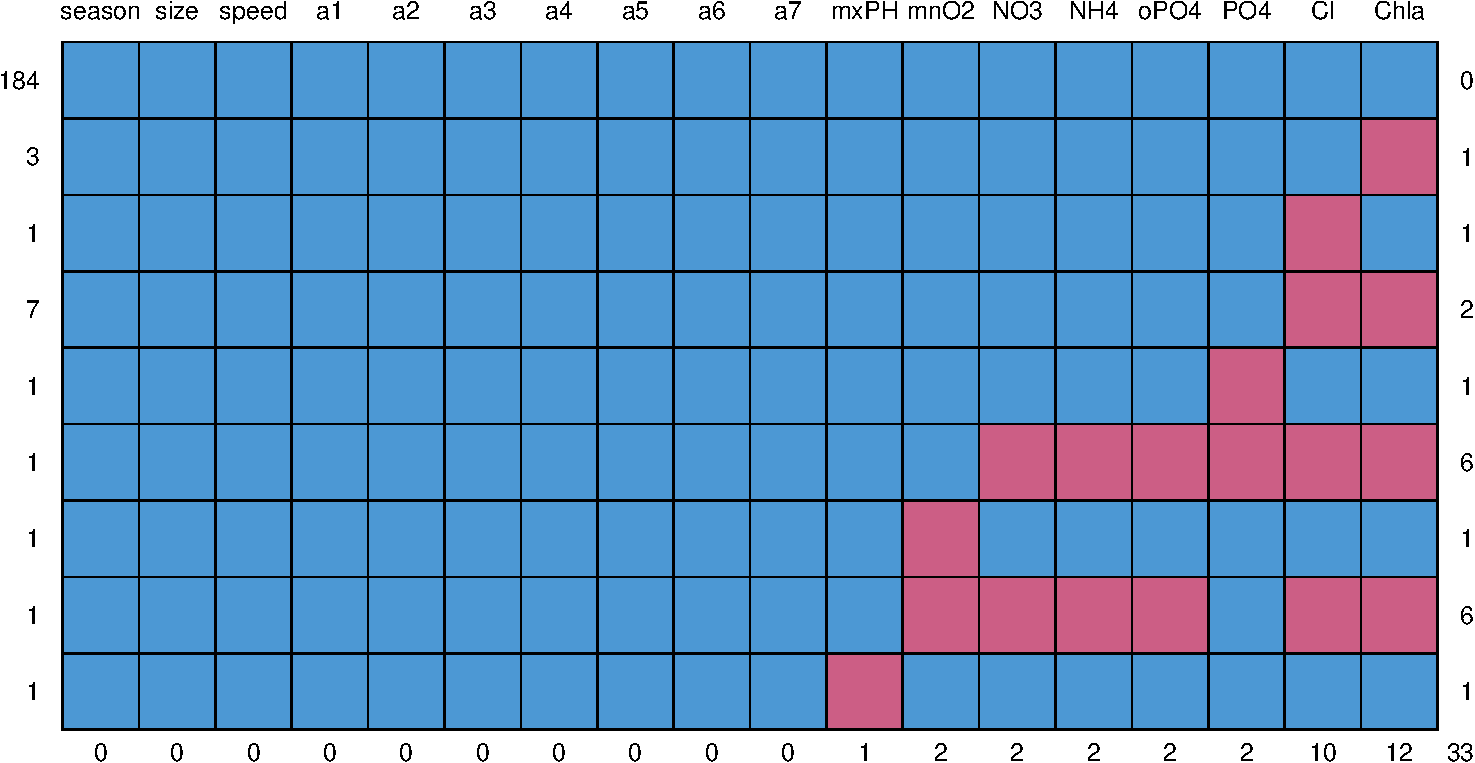
\includegraphics{EksploracjaDanych_files/figure-latex/mice1-1.pdf}
\caption{\label{fig:mice1}Na czerwono zaznaczone są zmienne, które zwierają braki danych. Liczba w wierszu po lewej stronie wykresu wskazuje ile wierszy w bazie ma daną charakterystykę, a liczba po prawej oznacza ile zmiennych było \emph{wybrakowanych}}
\end{figure}

\begin{verbatim}
##     season size speed a1 a2 a3 a4 a5 a6 a7 mxPH mnO2 NO3 NH4 oPO4 PO4 Cl
## 184      1    1     1  1  1  1  1  1  1  1    1    1   1   1    1   1  1
## 3        1    1     1  1  1  1  1  1  1  1    1    1   1   1    1   1  1
## 1        1    1     1  1  1  1  1  1  1  1    1    1   1   1    1   1  0
## 7        1    1     1  1  1  1  1  1  1  1    1    1   1   1    1   1  0
## 1        1    1     1  1  1  1  1  1  1  1    1    1   1   1    1   0  1
## 1        1    1     1  1  1  1  1  1  1  1    1    1   0   0    0   0  0
## 1        1    1     1  1  1  1  1  1  1  1    1    0   1   1    1   1  1
## 1        1    1     1  1  1  1  1  1  1  1    1    0   0   0    0   1  0
## 1        1    1     1  1  1  1  1  1  1  1    0    1   1   1    1   1  1
##          0    0     0  0  0  0  0  0  0  0    1    2   2   2    2   2 10
##     Chla   
## 184    1  0
## 3      0  1
## 1      1  1
## 7      0  2
## 1      1  1
## 1      0  6
## 1      1  1
## 1      0  6
## 1      1  1
##       12 33
\end{verbatim}

\hypertarget{zastepowanie-brakow-danych}{%
\section{Zastępowanie braków danych}\label{zastepowanie-brakow-danych}}

Zastępowanie braków danych (zwane także \emph{imputacją danych}) jest kolejnym etapem procesu przygotowania danych do analiz. Nie można jednak wyróżnić uniwersalnego sposobu zastępowania braków dla wszystkich możliwych sytuacji. Wśród statystyków panuje przekonanie, że w przypadku wystąpienia braków danych można zastosować trzy strategie:

\begin{itemize}
\tightlist
\item
  nic nie robić z brakami - co wydaje się niedorzeczne ale wcale takie nie jest, ponieważ istnieje wiele modeli statystycznych (np. drzewa decyzyjne), które świetnie radzą sobie w sytuacji braków danych. Niestety nie jest to sposób, który można stosować zawsze, ponieważ są również modele wymagające kompletności danych jak na przykład sieci neuronowe.
\item
  usuwać braki wierszami\footnote{polega na usuwaniu wierszy zawierających braki} - to metoda, która jest stosowana domyślnie w przypadku kiedy twórca modelu nie zadecyduje o innym sposobie obsługi luk. Metoda ta ma swoją niewątpliwą zaletę w postaci jasnej i prostej procedury, ale szczególnie w przypadku niewielkich zbiorów może skutkować obciążeniem estymatorów. Nie wiemy bowiem jaka wartość faktycznie jest przypisana danej cesze. Jeśli jest to wartość bliska np. średniej, to nie wpłynie znacząco na obciążenie estymatora wartości oczekiwanej. W przypadku, gdy różni się ona znacznie od średniej tej cechy, to estymator może już wykazywać obciążenie. Jego wielkość zależy również od liczby usuniętych elementów. Nie jest zalecane usuwanie wielu wierszy ze zbioru danych i na podstawie okrojonego zbioru wyciąganie wniosków o populacji, ponieważ próba jest wówczas znacząco inna niż populacja. Dodatkowo jeśli estymatory są wyznaczane na podstawie zbioru wyraźnie mniej licznego, to precyzja estymatorów wyrażona wariancją spada. Reasumując, jeśli liczba wierszy z brakującymi danymi jest niewielka w stosunku do całego zbioru, to usuwanie wierszy jest sensownym rozwiązaniem.
\item
  uzupełnianie braków - to procedura polegająca na zastępowaniu braków różnymi technikami. Jej niewątpliwą zaletą jest fakt posiadania kompletnych danych bez konieczności usuwania wierszy. Niestety wiąże się to również z pewnymi wadami. Zbiór posiadający wiele braków uzupełnianych nawet bardzo wyrafinowanymi metodami może cechować się zaniżoną wariancją poszczególnych cech oraz tzw. przeuczeniem\footnote{więcej o zjawisku przeuczenia w dalszej części książki}.
\end{itemize}

\begin{enumerate}
\def\labelenumi{\arabic{enumi}.}
\tightlist
\item
  Uzupełnianie średnią - braki w zakresie danej zmiennej uzupełniamy średnią tej zmiennej przypadków uzupełnionych.
\end{enumerate}

\begin{Shaded}
\begin{Highlighting}[]
\NormalTok{algae[}\KeywordTok{is.na}\NormalTok{(algae}\OperatorTok{$}\NormalTok{mxPH), ]}
\end{Highlighting}
\end{Shaded}

\begin{verbatim}
##    season  size speed mxPH mnO2 Cl  NO3 NH4 oPO4 PO4 Chla   a1 a2 a3 a4 a5
## 48 winter small   low   NA 12.6  9 0.23  10    5   6  1.1 35.5  0  0  0  0
##    a6 a7
## 48  0  0
\end{verbatim}

\begin{Shaded}
\begin{Highlighting}[]
\NormalTok{m <-}\StringTok{ }\KeywordTok{mean}\NormalTok{(algae}\OperatorTok{$}\NormalTok{mxPH, }\DataTypeTok{na.rm =}\NormalTok{ T)}
\NormalTok{algae[}\KeywordTok{is.na}\NormalTok{(algae}\OperatorTok{$}\NormalTok{mxPH), }\StringTok{"mxPH"}\NormalTok{] <-}\StringTok{ }\NormalTok{m}
\NormalTok{algae[}\KeywordTok{is.na}\NormalTok{(algae}\OperatorTok{$}\NormalTok{mxPH), ]}
\end{Highlighting}
\end{Shaded}

\begin{verbatim}
##  [1] season size   speed  mxPH   mnO2   Cl     NO3    NH4    oPO4   PO4   
## [11] Chla   a1     a2     a3     a4     a5     a6     a7    
## <0 rows> (or 0-length row.names)
\end{verbatim}

\begin{enumerate}
\def\labelenumi{\arabic{enumi}.}
\setcounter{enumi}{1}
\tightlist
\item
  Uzupełnianie medianą - braki w zakresie danej zmiennej uzupełniamy medianą tej zmiennej przypadków uzupełnionych.
\end{enumerate}

\begin{Shaded}
\begin{Highlighting}[]
\NormalTok{algae }\OperatorTok\StringTok{ }\KeywordTok{filter}\NormalTok{(}\KeywordTok{is.na}\NormalTok{(Chla)) }\OperatorTok\StringTok{ }\NormalTok{head}
\end{Highlighting}
\end{Shaded}

\begin{verbatim}
##   season  size  speed mxPH mnO2 Cl   NO3 NH4 oPO4  PO4 Chla   a1  a2  a3
## 1 winter small   high  6.6 10.8 NA 3.245  10    1  6.5   NA 24.3 0.0 0.0
## 2 spring small medium  5.6 11.8 NA 2.220   5    1  1.0   NA 82.7 0.0 0.0
## 3 autumn small medium  5.7 10.8 NA 2.550  10    1  4.0   NA 16.8 4.6 3.9
## 4 spring small   high  6.6  9.5 NA 1.320  20    1  6.0   NA 46.8 0.0 0.0
## 5 summer small   high  6.6 10.8 NA 2.640  10    2 11.0   NA 46.9 0.0 0.0
## 6 autumn small medium  6.6 11.3 NA 4.170  10    1  6.0   NA 47.1 0.0 0.0
##     a4 a5  a6 a7
## 1  0.0  0 0.0  0
## 2  0.0  0 0.0  0
## 3 11.5  0 0.0  0
## 4 28.8  0 0.0  0
## 5 13.4  0 0.0  0
## 6  0.0  0 1.2  0
\end{verbatim}

\begin{Shaded}
\begin{Highlighting}[]
\NormalTok{algae[}\KeywordTok{is.na}\NormalTok{(algae}\OperatorTok{$}\NormalTok{Chla), }\StringTok{"Chla"}\NormalTok{] <-}\StringTok{ }\KeywordTok{median}\NormalTok{(algae}\OperatorTok{$}\NormalTok{Chla, }\DataTypeTok{na.rm =}\NormalTok{ T)}
\end{Highlighting}
\end{Shaded}

\begin{enumerate}
\def\labelenumi{\arabic{enumi}.}
\setcounter{enumi}{2}
\tightlist
\item
  Wypełnianie zmiennych typu wyliczeniowego, logicznego lub znakowego odbywa się najczęściej przez dobranie w miejsce brakującej wartości, elementu powtarzającego się najczęściej wśród obiektów obserwowanych. W pakiecie \textbf{DMwR} istnieje funkcja \texttt{centralImputation}, która wypełnia braki wartością centralną (w przypadku zmiennych typu liczbowego - medianą, a dla wartości logicznych, wyliczeniowych lub tekstowych - modą).
\end{enumerate}

\begin{Shaded}
\begin{Highlighting}[]
\NormalTok{algae[}\DecValTok{48}\NormalTok{, }\StringTok{"season"}\NormalTok{]}
\end{Highlighting}
\end{Shaded}

\begin{verbatim}
## [1] "winter"
\end{verbatim}

\begin{Shaded}
\begin{Highlighting}[]
\NormalTok{algae[}\DecValTok{48}\NormalTok{, }\StringTok{"season"}\NormalTok{] <-}\StringTok{ }\OtherTok{NA}
\NormalTok{algae.uzup <-}\StringTok{ }\KeywordTok{centralImputation}\NormalTok{(algae)}
\NormalTok{algae.uzup[}\DecValTok{48}\NormalTok{,]}
\end{Highlighting}
\end{Shaded}

\begin{verbatim}
##    season  size speed     mxPH mnO2 Cl  NO3 NH4 oPO4 PO4 Chla   a1 a2 a3
## 48 winter small   low 8.011734 12.6  9 0.23  10    5   6  1.1 35.5  0  0
##    a4 a5 a6 a7
## 48  0  0  0  0
\end{verbatim}

\begin{enumerate}
\def\labelenumi{\arabic{enumi}.}
\setcounter{enumi}{3}
\tightlist
\item
  Jeszcze innym sposobem imputacji danych są algorytmy oparte o metodę \(k\)-najbliższych sąsiadów. Algorytm opiera się na prostej zasadzie, uzupełniania brakujących wartości medianą (w przypadku zmiennych ilościowych) lub modą (w przypadku zmiennych jakościowych) elementów, które są \(k\)-tymi najbliższymi sąsiadami w metryce
  \begin{equation}\label{knn}
   d(x,y)=\sqrt{\sum_{i=1}^{p}\delta_i(x_i,y_i)},
  \end{equation}
  gdzie \(\delta_i\) jest odległością pomiędzy dwoma elementami ze względu na \(i\)-tą cech, określoną następująco
  \begin{equation}\label{metryka}
   \delta_i(v_1, v_2)=\begin{cases}
       1,& \text{jeśli zmienna jest jakościowa i }v_1\neq v_2\\
       0,& \text{jeśli zmienna jest jakościowa i }v_1=v_2\\
       (v_1-v_2)^2,& \text{jeśli zmienna jest ilościowa.}
   \end{cases}
  \end{equation}
  Odległości są mierzone dla zmiennych standaryzowanych. Istnieje też odmiana z wagami, które maleją wraz ze wzrostem odległości pomiędzy sąsiadem a uzupełnianym elementem (np. \(w(d)=\exp(d)\)).
\end{enumerate}

\begin{Shaded}
\begin{Highlighting}[]
\NormalTok{algae[}\DecValTok{48}\NormalTok{, ]}
\end{Highlighting}
\end{Shaded}

\begin{verbatim}
##    season  size speed     mxPH mnO2 Cl  NO3 NH4 oPO4 PO4 Chla   a1 a2 a3
## 48   <NA> small   low 8.011734 12.6  9 0.23  10    5   6  1.1 35.5  0  0
##    a4 a5 a6 a7
## 48  0  0  0  0
\end{verbatim}

\begin{Shaded}
\begin{Highlighting}[]
\NormalTok{algae <-}\StringTok{ }\NormalTok{algae }\OperatorTok\StringTok{ }
\StringTok{    }\KeywordTok{mutate_if}\NormalTok{(is.character, as.factor)}
\NormalTok{algae.uzup <-}\StringTok{ }\KeywordTok{knnImputation}\NormalTok{(algae, }\DataTypeTok{k =} \DecValTok{5}\NormalTok{, }\DataTypeTok{scale =}\NormalTok{ F, }\DataTypeTok{meth =} \StringTok{"median"}\NormalTok{)}
\NormalTok{algae.uzup[}\DecValTok{48}\NormalTok{,]}
\end{Highlighting}
\end{Shaded}

\begin{verbatim}
##    season  size speed     mxPH mnO2 Cl  NO3 NH4 oPO4 PO4 Chla   a1 a2 a3
## 48 summer small   low 8.011734 12.6  9 0.23  10    5   6  1.1 35.5  0  0
##    a4 a5 a6 a7
## 48  0  0  0  0
\end{verbatim}

Istnieją również dużo bardziej złożone algorytmy imputacji danych oparte na bardziej wyrafinowanych technikach, takich jak: predykcja modelami liniowymi, nieliniowymi, analiza dyskryminacyjna, drzewa klasyfikacyjne. Dwa najbardziej znane pakiety zawierające funkcje do imputacji w sposób złożony, to \textbf{Amelia} i \textbf{mice}.

Imputacja danych z zastosowaniem pakietu \textbf{mice} wymaga podjęcia kilku decyzji przed przystąpieniem do uzupełniania danych:

\begin{enumerate}
\def\labelenumi{\arabic{enumi}.}
\tightlist
\item
  Czy dane są MAR (ang. \emph{Missing At Random}) czy MNAR (ang. \emph{Missing Not At Random}), co oznacza, że musimy się zastanowić jakie mogły być źródła braków danych, przypadkowe czy systematyczne?
\item
  Należy się zdecydować na formę imputacji, określając strukturę zależności pomiędzy cechami oraz rozkład błędu danej cechy?
\item
  Wybrać zbiór danych, który posłuży nam za predyktory w imputacji (nie mogą zawierać braków).
\item
  Określenie, które niepełne zmienne są funkcjami innych wybrakowanych zmiennych.
\item
  Określić w jakiej kolejności dane będą imputowane.
\item
  Określić parametry startowe imputacji (liczbę iteracji, warunek zbieżności).
\item
  Określić liczę imputowanych zbiorów.
\end{enumerate}

Ad 1. Wyróżniamy następujące rodzaje braków danych:

\begin{itemize}
\tightlist
\item
  MCAR (ang. \emph{Missing Completely At Random}) - z definicji to braki, których pojawienie się jest kompletnie losowe. Przykładowo gdy osoba poproszona o wypełnienie wieku w ankiecie będzie rzucać monetą czy wypełnić tą zmienną.
\item
  MAR - oznacza, że obserwowane wartości i wybrakowane mają inne rozkłady ale da się je oszacować na podstawie danych obserwowanych. Przykładowo ciśnienie tętnicze u osób, które nie wypełniły tej wartości jest wyższe niż u osób, które wpisały swoje ciśnienie. Okazuje się, że osoby starsze z nadciśnieniem nie wypełniały ankiety w tym punkcie.
\item
  MNAR - jeśli nie jest spełniony warunek MCAR i MAR, wówczas brak ma charakter nielosowy. Przykładowo respondenci osiągający wyższe zarobki sukcesywnie nie wypełniają pola ``zarobki'' i dodatkowo nie ma w ankiecie zmiennych, które pozwoliłyby nam ustalić, jakie to osoby.
\end{itemize}

Ad 2. Decyzja o algorytmie imputacji wynika bezpośrednio ze skali w jakiej jest mierzona dana zmienna. Ze względu na rodzaj cechy używać będziemy następujących metod:

\begin{table}[t]

\caption{\label{tab:methods}Zestaw metod imputacji danych stosowanych w pakiecie **mice**}
\centering
\begin{tabular}{lll}
\toprule
method & type & description\\
\midrule
pmm & any & Predictive.mean.matching\\
midastouch & any & Weighted predictive mean matching\\
sample & any & Random sample from observed values\\
cart & any & Classification and regression trees\\
rf & any & Random forest imputations\\
\addlinespace
mean & numeric & Unconditional mean imputation\\
norm & numeric & Bayesian linear regression\\
norm.nob & numeric & Linear regression ignoring model error\\
norm.boot & numeric & Linear regression using bootstrap\\
norm.predict & numeric & Linear regression, predicted values\\
\addlinespace
quadratic & numeric & Imputation of quadratic terms\\
ri & numeric & Random indicator for nonignorable data\\
logreg & binary & Logistic regression\\
logreg.boot & binary & Logistic regression with bootstrap\\
polr & ordered & Proportional odds model\\
\addlinespace
polyreg & unordered & Polytomous logistic regression\\
lda & unordered & Linear discriminant analysis\\
2l.norm & numeric & Level-1 normal heteroscedastic\\
2l.lmer & numeric & Level-1 normal homoscedastic,
                                lmer\\
2l.pan & numeric & Level-1 normal homoscedastic, pan\\
\addlinespace
2l.bin & binary & Level-1 logistic, glmer\\
2lonly.mean & numeric & Level-2 class mean\\
2lonly.norm & numeric & Level-2 class normal\\
2lonly.pmm & any & Level-2 class predictive mean matching\\
\bottomrule
\end{tabular}
\end{table}

Każdy z czterech typów danych ma swój domyślny algorytm przeznaczony do imputacji:

\begin{itemize}
\tightlist
\item
  zmienna ilościowa - \texttt{pmm}
\item
  zmienna dychotomiczna (stany 0 lub 1) - \texttt{logreg}
\item
  zmienna typu wyliczeniowego (nieuporządkowana) - \texttt{polyreg}
\item
  zmienna typu wyliczeniowego (uporządkowana) - \texttt{polr}
\end{itemize}

Niewątpliwą zaletą metody \texttt{pmm} jest to, że wartości imputowane są ograniczone jedynie do obserwowanych wartości. Metody \texttt{norm} i \texttt{norm.nob} uzupełniają brakujące wartości w oparciu o model liniowy. Są one szybkie i efektywne w przypadku gdy reszty modelu są zbliżone rozkładem do normalności. Druga z tych technik nie bierze pod uwagę niepewności związanej z modelem imputującym. Metoda \texttt{2L.norm} opiera się na dwupoziomowym heterogenicznym modelu liniowym (skupienia są włączone jako efekt do modelu). Technika \texttt{polyreg} korzysta z funkcji \texttt{multinom} pakietu \textbf{nnet} tworzącej model wielomianowy. \texttt{polr} opiera się o proporcjonalny model logitowy z pakietu \textbf{MASS}. \texttt{lda} to model dyskryminacyjny klasyfikujący obiekty na podstawie prawdopodobieństw \emph{a posteriori}. Metoda \texttt{sample} zastępuje braki losowa wybranymi wartościami spośród wartości obserwowanych.

Ad 3. Do ustalenia predyktorów w modelu \texttt{mice} służy funkcja \texttt{predictorMatrix}. Po pierwsze wyświetla ona domyślny układ predyktorów włączanych do modelu. Można go dowolnie zmienić i podstawić do modelu imputującego dane parametrem \texttt{predictorMatrix}. Zera występujące w kolejnych wierszach macierzy predyktorów oznaczają pominięcie tej zmiennej przy imputacji innej zmiennej. Jeśli dodatkowo chcemy by jakaś zmienna nie była imputowana, to oprócz usunięcia jej z listy predyktorów, należy wymazać ją z listy metod predykcji (\texttt{method}).

Ogólne zalecenia co do tego jakie zmienne stosować jako predyktory jest takie, żeby brać ich jak najwięcej. Spowoduje to, że bardziej prawdopodobny staje się brak typu MAR a nie MNAR. Z drugiej jednak strony, nierzadko zbiory zawierają olbrzymią liczbę zmiennych i włączanie ich wszystkich do modelu imputującego nie będzie miało sensu.

Zalecenia doboru zmiennych są następujące:

\begin{itemize}
\tightlist
\item
  weź wszystkie te zmienne, które są włączane do modelu właściwego, czyli tego za pomocą którego chcesz poznać strukturę zależności;
\item
  czasem do modelu imputującego należy też włączyć interakcje zmiennych z modelu właściwego;
\item
  dodaj zmienne, które mogą mieć wpływ na wybrakowane cechy;
\item
  włącz zmienne istotnie podnoszące poziom wyjaśnionej wariancji modelu;
\item
  na koniec usuń te zmienne spośród predyktorów, które same zawierają zbyt wiele braków.
\end{itemize}

Ad 4-7. Decyzje podejmowane w tych punktach zależą istotnie od analizowanego zbioru i będą przedmiotem oddzielnych analiz w kontekście rozważanych zbiorów i zadań.

\BeginKnitrBlock{example}
\protect\hypertarget{exm:przyk21}{}{\label{exm:przyk21} }Dokonamy imputacji zbioru \texttt{airquality} z wykorzystaniem pakietów \textbf{mice} i \textbf{VIM} (Templ et al. \protect\hyperlink{ref-R-VIM}{2019})
\EndKnitrBlock{example}

\begin{Shaded}
\begin{Highlighting}[]
\NormalTok{data <-}\StringTok{ }\NormalTok{airquality}
\KeywordTok{summary}\NormalTok{(data)}
\end{Highlighting}
\end{Shaded}

\begin{verbatim}
##      Ozone           Solar.R           Wind             Temp      
##  Min.   :  1.00   Min.   :  7.0   Min.   : 1.700   Min.   :56.00  
##  1st Qu.: 18.00   1st Qu.:115.8   1st Qu.: 7.400   1st Qu.:72.00  
##  Median : 31.50   Median :205.0   Median : 9.700   Median :79.00  
##  Mean   : 42.13   Mean   :185.9   Mean   : 9.958   Mean   :77.88  
##  3rd Qu.: 63.25   3rd Qu.:258.8   3rd Qu.:11.500   3rd Qu.:85.00  
##  Max.   :168.00   Max.   :334.0   Max.   :20.700   Max.   :97.00  
##  NA's   :37       NA's   :7                                       
##      Month            Day      
##  Min.   :5.000   Min.   : 1.0  
##  1st Qu.:6.000   1st Qu.: 8.0  
##  Median :7.000   Median :16.0  
##  Mean   :6.993   Mean   :15.8  
##  3rd Qu.:8.000   3rd Qu.:23.0  
##  Max.   :9.000   Max.   :31.0  
## 
\end{verbatim}

\begin{Shaded}
\begin{Highlighting}[]
\CommentTok{# tworzymy dodatkowe braki danych}
\NormalTok{data[}\DecValTok{4}\OperatorTok{:}\DecValTok{10}\NormalTok{,}\DecValTok{3}\NormalTok{] <-}\StringTok{ }\KeywordTok{rep}\NormalTok{(}\OtherTok{NA}\NormalTok{,}\DecValTok{7}\NormalTok{)}
\NormalTok{data[}\DecValTok{1}\OperatorTok{:}\DecValTok{5}\NormalTok{,}\DecValTok{4}\NormalTok{] <-}\StringTok{ }\OtherTok{NA}
\KeywordTok{summary}\NormalTok{(data)}
\end{Highlighting}
\end{Shaded}

\begin{verbatim}
##      Ozone           Solar.R           Wind             Temp      
##  Min.   :  1.00   Min.   :  7.0   Min.   : 1.700   Min.   :57.00  
##  1st Qu.: 18.00   1st Qu.:115.8   1st Qu.: 7.400   1st Qu.:73.00  
##  Median : 31.50   Median :205.0   Median : 9.700   Median :79.00  
##  Mean   : 42.13   Mean   :185.9   Mean   : 9.806   Mean   :78.28  
##  3rd Qu.: 63.25   3rd Qu.:258.8   3rd Qu.:11.500   3rd Qu.:85.00  
##  Max.   :168.00   Max.   :334.0   Max.   :20.700   Max.   :97.00  
##  NA's   :37       NA's   :7       NA's   :7        NA's   :5      
##      Month            Day      
##  Min.   :5.000   Min.   : 1.0  
##  1st Qu.:6.000   1st Qu.: 8.0  
##  Median :7.000   Median :16.0  
##  Mean   :6.993   Mean   :15.8  
##  3rd Qu.:8.000   3rd Qu.:23.0  
##  Max.   :9.000   Max.   :31.0  
## 
\end{verbatim}

\begin{Shaded}
\begin{Highlighting}[]
\KeywordTok{md.pattern}\NormalTok{(data)}
\end{Highlighting}
\end{Shaded}

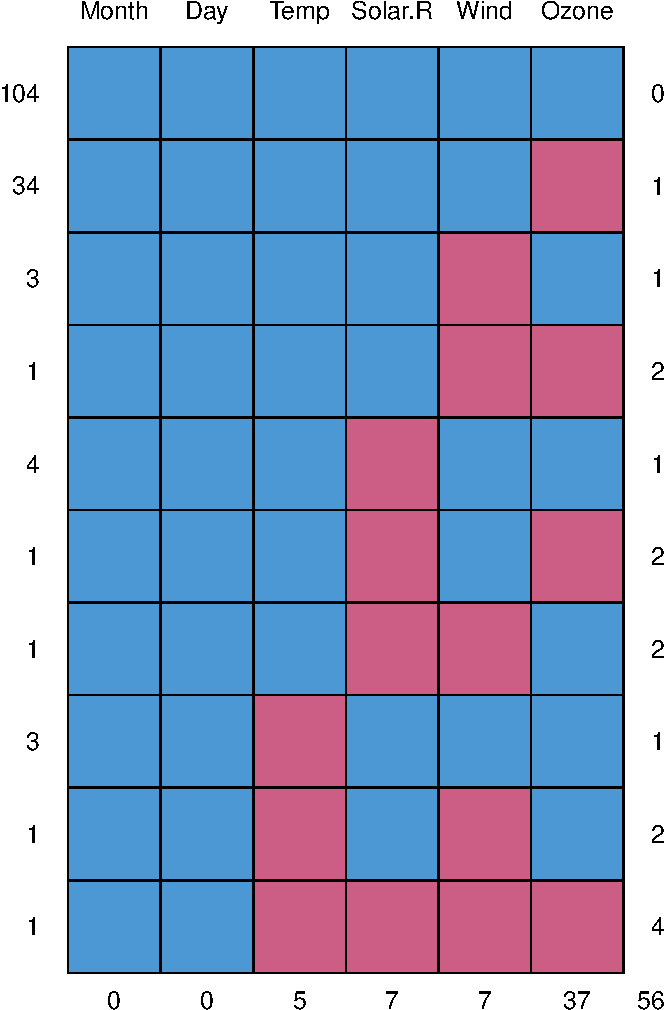
\includegraphics{EksploracjaDanych_files/figure-latex/unnamed-chunk-3-1.pdf}

\begin{verbatim}
##     Month Day Temp Solar.R Wind Ozone   
## 104     1   1    1       1    1     1  0
## 34      1   1    1       1    1     0  1
## 3       1   1    1       1    0     1  1
## 1       1   1    1       1    0     0  2
## 4       1   1    1       0    1     1  1
## 1       1   1    1       0    1     0  2
## 1       1   1    1       0    0     1  2
## 3       1   1    0       1    1     1  1
## 1       1   1    0       1    0     1  2
## 1       1   1    0       0    0     0  4
##         0   0    5       7    7    37 56
\end{verbatim}

Do ilustracji braków danych można zastosować funkcje pakietu \textbf{VIM}.

\begin{Shaded}
\begin{Highlighting}[]
\KeywordTok{library}\NormalTok{(VIM)}
\KeywordTok{aggr}\NormalTok{(data, }\DataTypeTok{numbers=}\OtherTok{TRUE}\NormalTok{, }
     \DataTypeTok{sortVars=}\OtherTok{TRUE}\NormalTok{, }
     \DataTypeTok{labels=}\KeywordTok{names}\NormalTok{(data), }
     \DataTypeTok{cex.axis=}\NormalTok{.}\DecValTok{7}\NormalTok{)}
\end{Highlighting}
\end{Shaded}

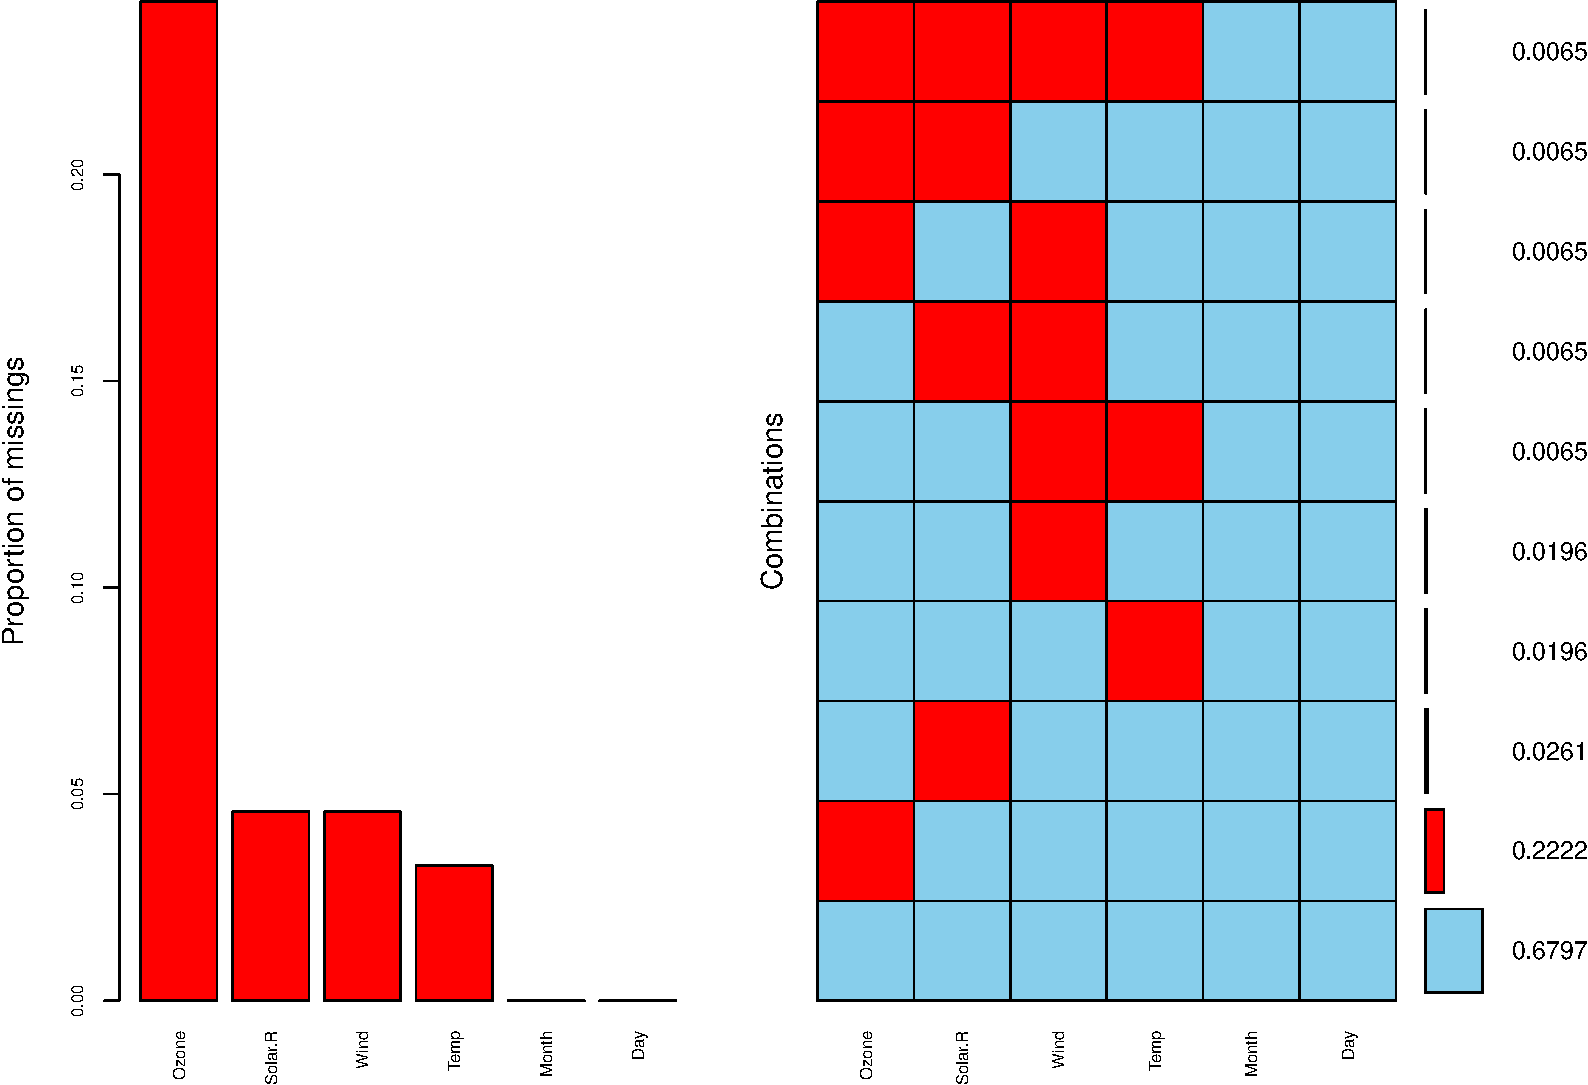
\includegraphics{EksploracjaDanych_files/figure-latex/unnamed-chunk-4-1.pdf}

\begin{verbatim}
## 
##  Variables sorted by number of missings: 
##  Variable      Count
##     Ozone 0.24183007
##   Solar.R 0.04575163
##      Wind 0.04575163
##      Temp 0.03267974
##     Month 0.00000000
##       Day 0.00000000
\end{verbatim}

Tak przedstawia się wykres rozrzutu zmiennych \texttt{Ozone} i \texttt{Solar.R} z uwzględnieniem położenia braków danych.

\begin{Shaded}
\begin{Highlighting}[]
\KeywordTok{marginplot}\NormalTok{(data[}\KeywordTok{c}\NormalTok{(}\DecValTok{1}\NormalTok{,}\DecValTok{2}\NormalTok{)])}
\end{Highlighting}
\end{Shaded}

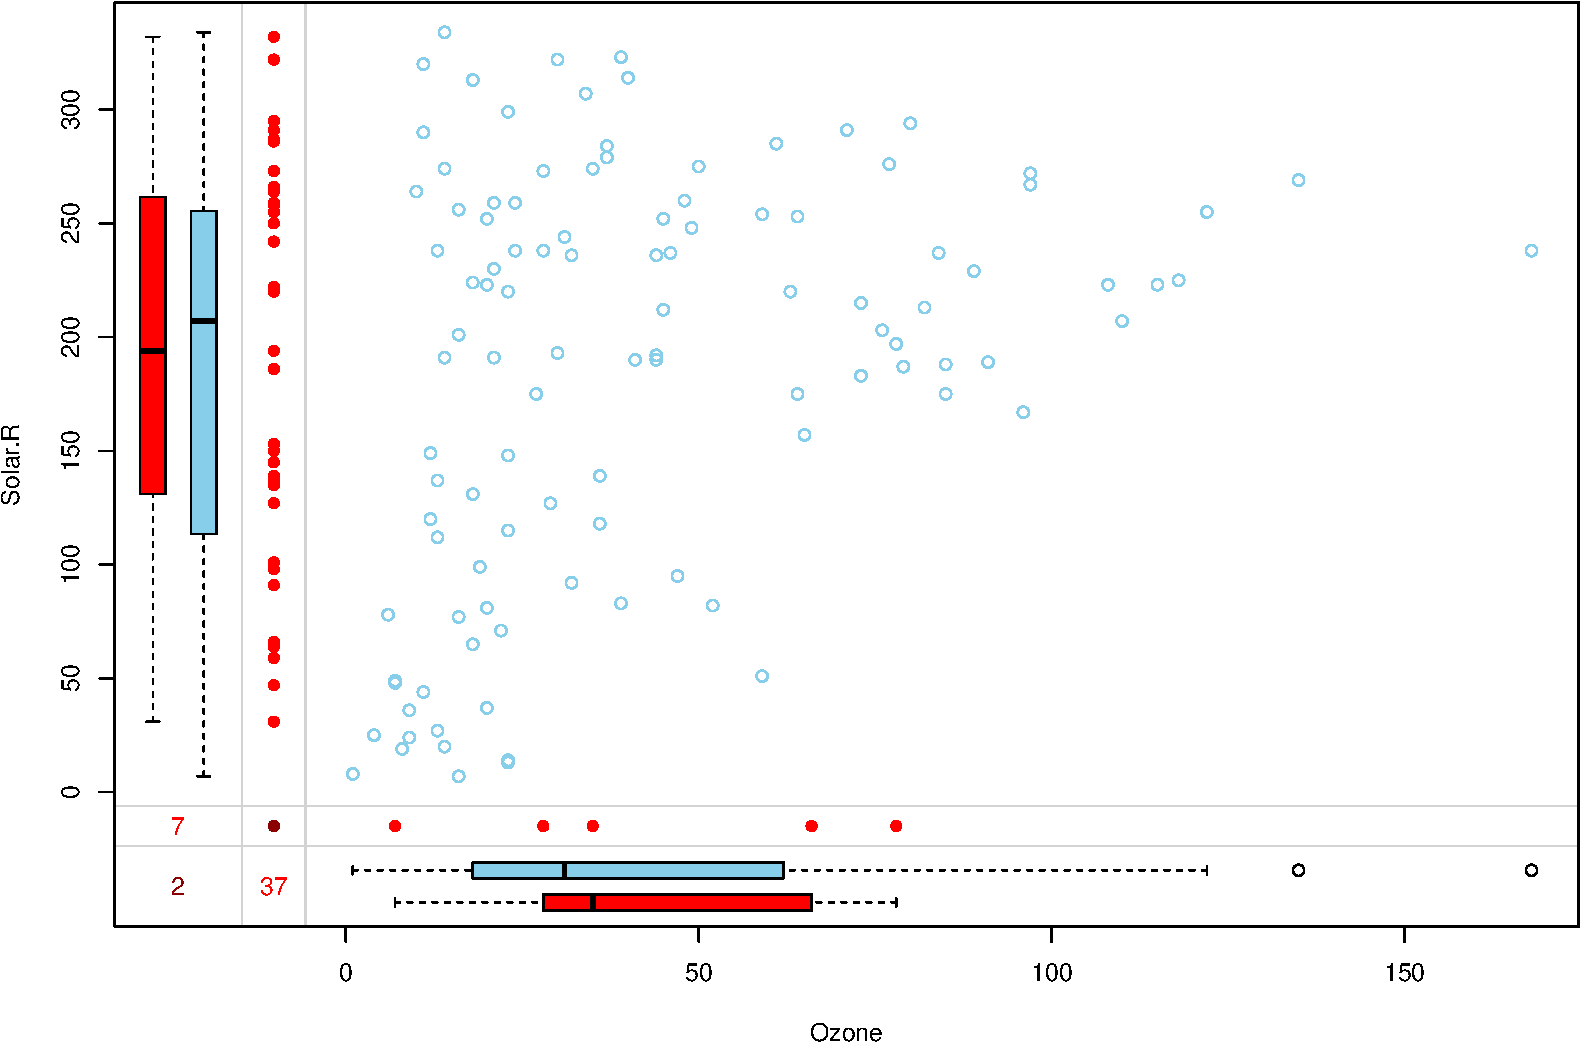
\includegraphics{EksploracjaDanych_files/figure-latex/unnamed-chunk-5-1.pdf}

Dokonamy imputacji metodą \texttt{pmm}.

\begin{Shaded}
\begin{Highlighting}[]
\NormalTok{tempData <-}\StringTok{ }\KeywordTok{mice}\NormalTok{(data, }
                 \DataTypeTok{maxit=}\DecValTok{50}\NormalTok{, }
                 \DataTypeTok{meth=}\StringTok{'pmm'}\NormalTok{, }
                 \DataTypeTok{seed=}\DecValTok{44}\NormalTok{, }
                 \DataTypeTok{printFlag =}\NormalTok{ F)}
\KeywordTok{summary}\NormalTok{(tempData)}
\end{Highlighting}
\end{Shaded}

\begin{verbatim}
## Class: mids
## Number of multiple imputations:  5 
## Imputation methods:
##   Ozone Solar.R    Wind    Temp   Month     Day 
##   "pmm"   "pmm"   "pmm"   "pmm"      ""      "" 
## PredictorMatrix:
##         Ozone Solar.R Wind Temp Month Day
## Ozone       0       1    1    1     1   1
## Solar.R     1       0    1    1     1   1
## Wind        1       1    0    1     1   1
## Temp        1       1    1    0     1   1
## Month       1       1    1    1     0   1
## Day         1       1    1    1     1   0
\end{verbatim}

Ponieważ, funkcja \texttt{mice} domyślnie dokonuje 5 kompletnych imputacji, możemy się przekonać jak bardzo różnią się poszczególne imputacje i zdecydować się na jedną z nich.

\begin{Shaded}
\begin{Highlighting}[]
\KeywordTok{head}\NormalTok{(tempData}\OperatorTok{$}\NormalTok{imp}\OperatorTok{$}\NormalTok{Ozone)}
\end{Highlighting}
\end{Shaded}

\begin{verbatim}
##     1  2  3  4  5
## 5  21 20  7 36 13
## 10 21 16 44 22 21
## 25 14 14 14  6  8
## 26 23 18  8 19 14
## 27 37 23 21  7  9
## 32 63 23  7 52 39
\end{verbatim}

Ostatecznie imputacji dokonujemy wybierając jeden z zestawów danych uzupełniających (np. pierwszy).

\begin{Shaded}
\begin{Highlighting}[]
\NormalTok{completedData <-}\StringTok{ }\NormalTok{mice}\OperatorTok{::}\KeywordTok{complete}\NormalTok{(tempData, }\DecValTok{1}\NormalTok{)}
\KeywordTok{summary}\NormalTok{(completedData)}
\end{Highlighting}
\end{Shaded}

\begin{verbatim}
##      Ozone          Solar.R           Wind             Temp      
##  Min.   :  1.0   Min.   :  7.0   Min.   : 1.700   Min.   :57.00  
##  1st Qu.: 20.0   1st Qu.:115.0   1st Qu.: 7.400   1st Qu.:73.00  
##  Median : 32.0   Median :212.0   Median : 9.700   Median :79.00  
##  Mean   : 42.5   Mean   :187.9   Mean   : 9.931   Mean   :78.14  
##  3rd Qu.: 59.0   3rd Qu.:259.0   3rd Qu.:11.500   3rd Qu.:85.00  
##  Max.   :168.0   Max.   :334.0   Max.   :20.700   Max.   :97.00  
##      Month            Day      
##  Min.   :5.000   Min.   : 1.0  
##  1st Qu.:6.000   1st Qu.: 8.0  
##  Median :7.000   Median :16.0  
##  Mean   :6.993   Mean   :15.8  
##  3rd Qu.:8.000   3rd Qu.:23.0  
##  Max.   :9.000   Max.   :31.0
\end{verbatim}

Za pomocą funkcji pakietu \texttt{mice} możemy również przedstawić graficznie gdzie i jak zostały uzupełnione dane.

\begin{Shaded}
\begin{Highlighting}[]
\KeywordTok{densityplot}\NormalTok{(tempData, }\OperatorTok{~}\NormalTok{Ozone}\OperatorTok{+}\NormalTok{Solar.R}\OperatorTok{+}\NormalTok{Wind}\OperatorTok{+}\NormalTok{Temp)}
\end{Highlighting}
\end{Shaded}

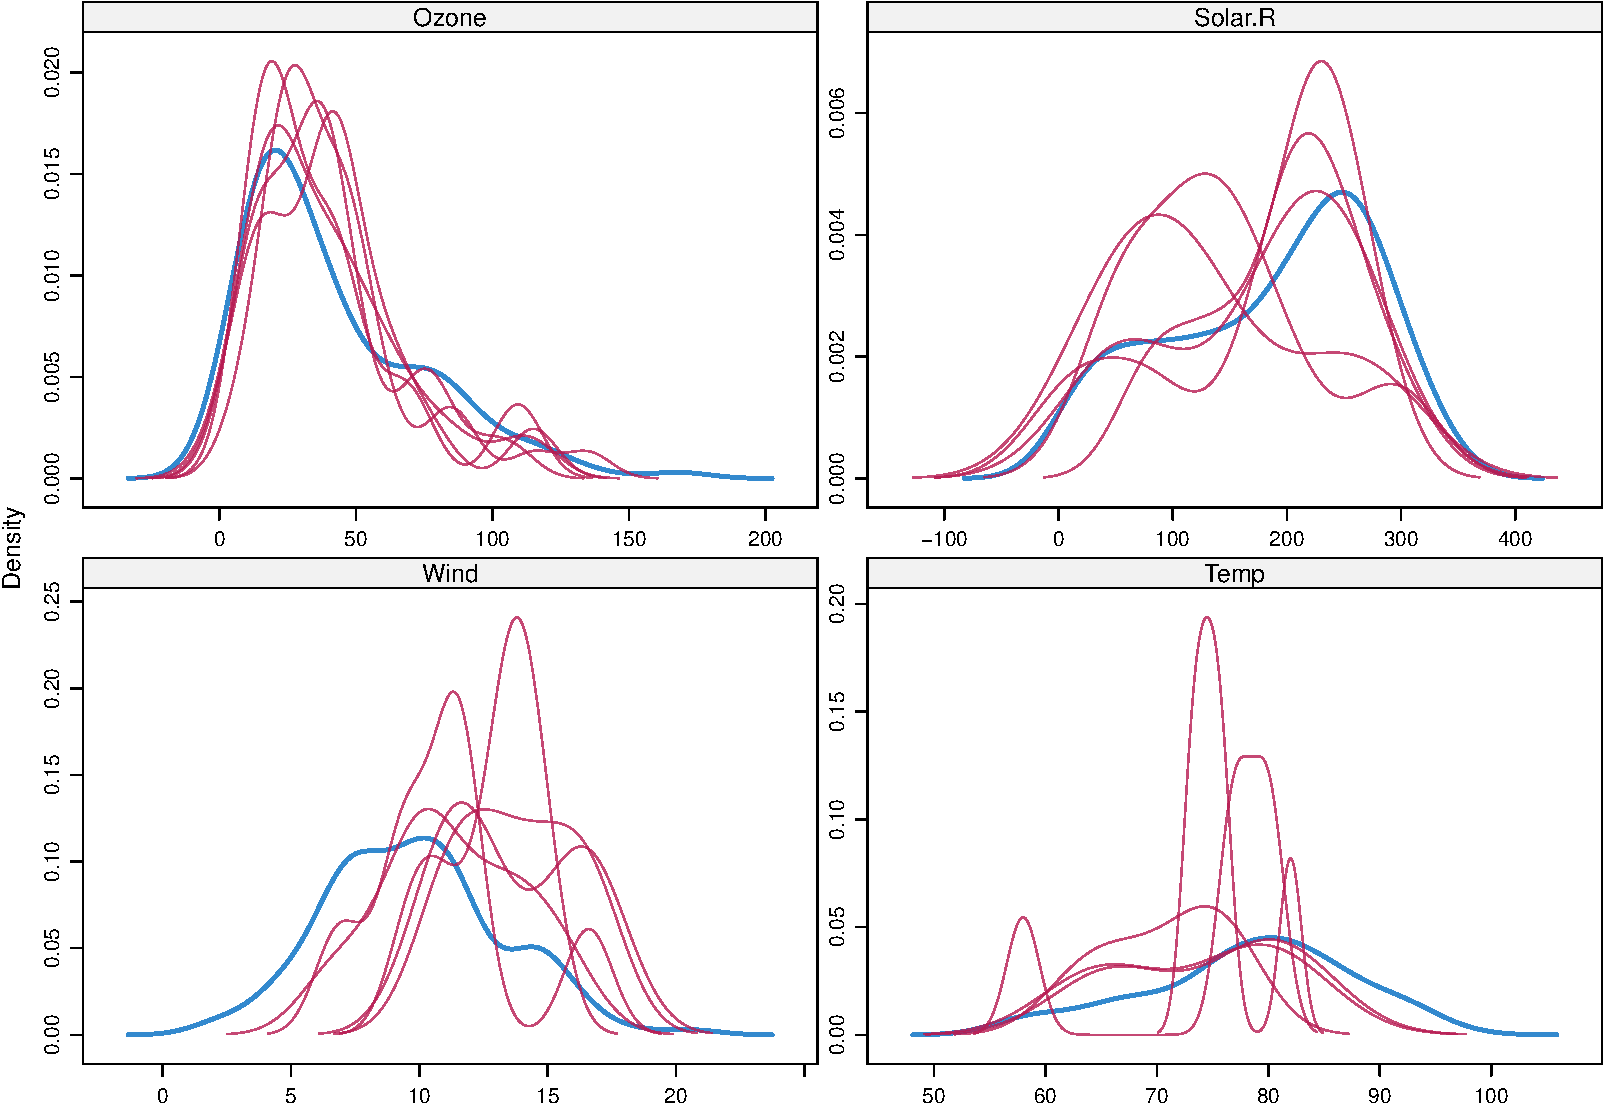
\includegraphics{EksploracjaDanych_files/figure-latex/unnamed-chunk-9-1.pdf}

\begin{Shaded}
\begin{Highlighting}[]
\KeywordTok{stripplot}\NormalTok{(tempData, Ozone}\OperatorTok{+}\NormalTok{Solar.R}\OperatorTok{+}\NormalTok{Wind}\OperatorTok{+}\NormalTok{Temp}\OperatorTok{~}\NormalTok{.imp, }\DataTypeTok{pch =} \DecValTok{20}\NormalTok{, }\DataTypeTok{cex =} \FloatTok{1.2}\NormalTok{)}
\end{Highlighting}
\end{Shaded}

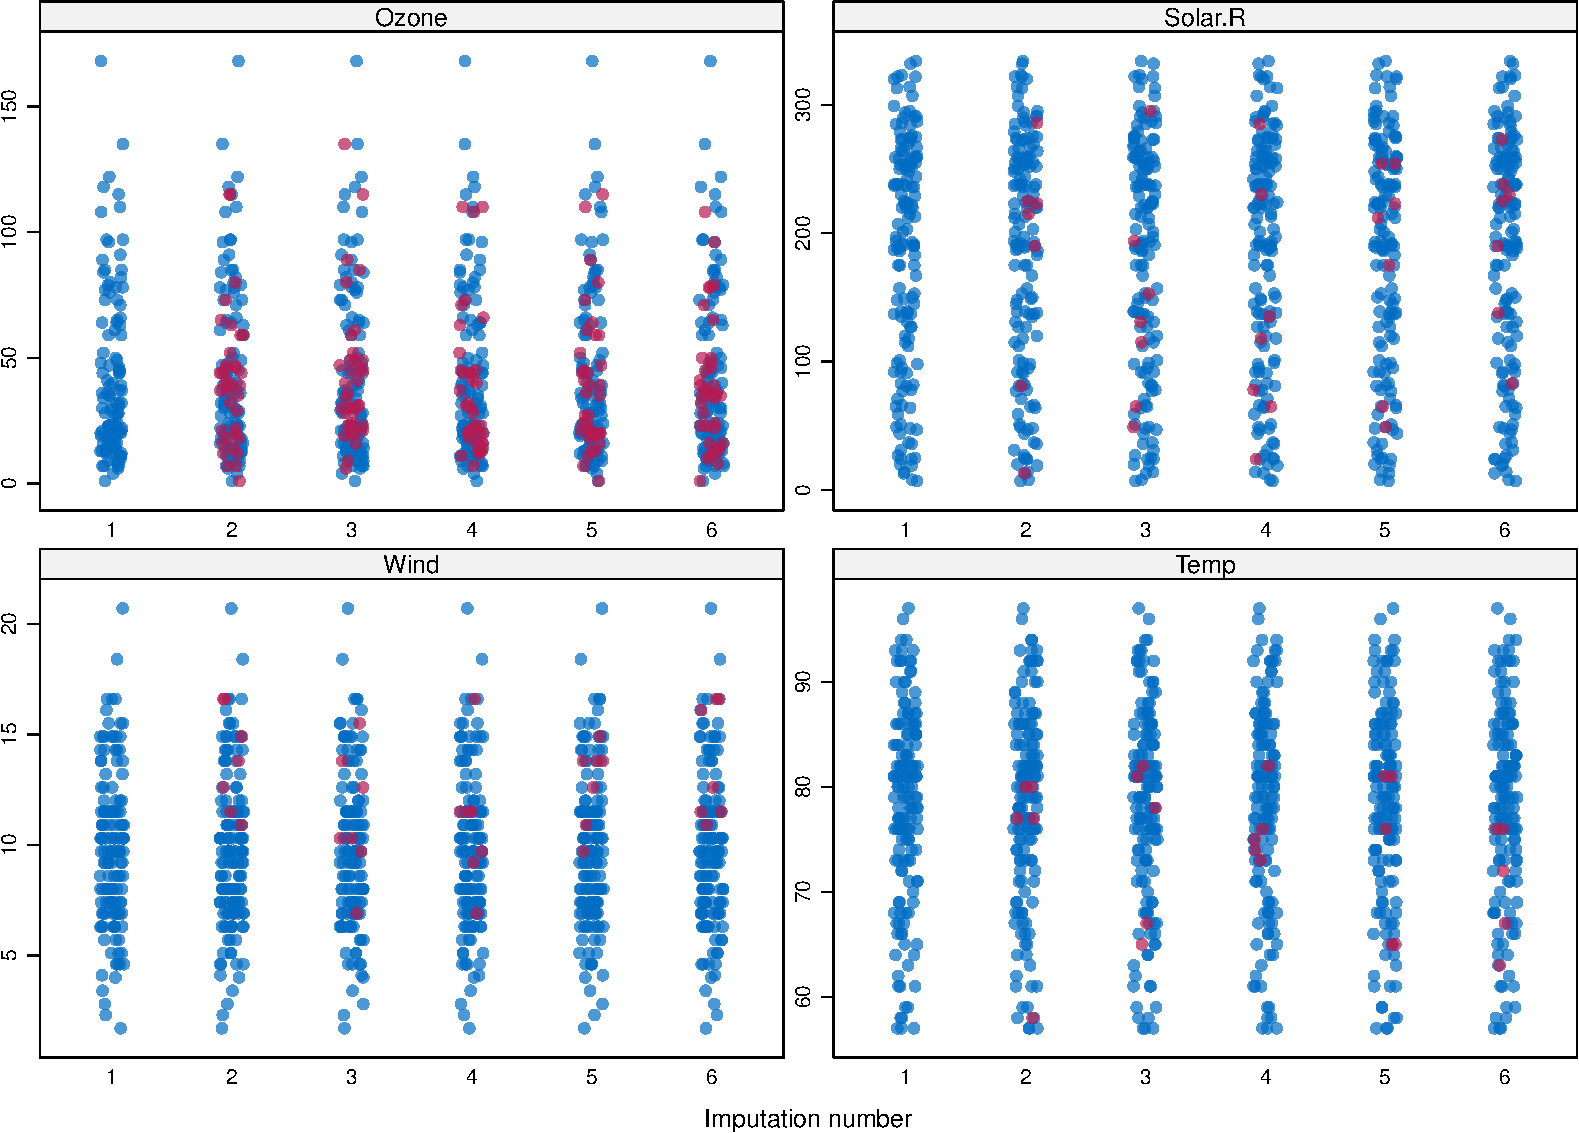
\includegraphics{EksploracjaDanych_files/figure-latex/unnamed-chunk-9-2.pdf}

\hypertarget{podzia-metod-data-mining}{%
\chapter{Podział metod data mining}\label{podzia-metod-data-mining}}

\hypertarget{rodzaje-wnioskowania}{%
\section{Rodzaje wnioskowania}\label{rodzaje-wnioskowania}}

\emph{Data mining} to zestaw metod pozyskiwania wiedzy na podstawie danych. Ową wiedzę zdobywamy w procesie wnioskowania na podstawie modeli. Wnioskowanie możemy podzielić na dedukcyjne i indukcyjne. I tak z wnioskowaniem dedukcyjnym mamy do czynienia wówczas, gdy na podstawie obecnego stanu wiedzy potrafimy odpowiedzieć na postawione pytanie dotyczące nowej wiedzy, stosując reguły wnioskowania. O wnioskowaniem indukcyjnym powiemy, że jest to metoda pozyskiwania wiedzy na podstawie informacji ze zbioru uczącego. Znajduje ono szerokie zastosowanie w data mining i charakteryzuje się omylnością, ponieważ nawet najlepiej nauczony model na zbiorze uczącym nie zapewnia nam prawdziwości odpowiedzi w przypadku nowych danych, a jedynie je uprawdopodabnia. Esencją wnioskowania indukcyjnego w zakresie data mining, jest poszukiwanie na podstawie danych uczących modelu charakteryzującego się najlepszymi właściwościami predykcyjnymi i dającego się zastosować do zupełnie nowego zbioru danych.

Każdy proces uczenia z wykorzystaniem wnioskowania indukcyjnego składa się z następujących elementów.

\hypertarget{dziedzina}{%
\subsection{Dziedzina}\label{dziedzina}}

\emph{Dziedzina} to zbiór wszystkich obiektów pozostających w zainteresowaniu badacza, będących przedmiotem wnioskowania, oznaczana najczęściej przez \(X\). Przykładowo mogą to być zbiory osób, transakcji, urządzeń, instytucji, itp.

\hypertarget{obserwacja}{%
\subsection{Obserwacja}\label{obserwacja}}

Każdy element dziedziny \(x\in X\) nazywamy obserwacją. Obserwacją nazywać będziemy zarówno rekordy danych ze zbioru uczącego, jak i ze zbioru testowego.

\hypertarget{atrybuty-obserwacji}{%
\subsection{Atrybuty obserwacji}\label{atrybuty-obserwacji}}

Każdy obiekt z dziedziny \(x\in X\) można opisać zestawem cech (atrybutów), które w notacji matematycznej oznaczymy przez \(a:X\to A\), gdzie \(A\) jest przestrzenią wartości atrybutów. Każda obserwacja \(x\) posiadająca \(k\) cech da się wyrazić wektorowo jako \((a_1(x), a_2(x), \ldots, a_k(x))\). Dla większości algorytmów uczenia maszynowego wyróżnia się trzy typy atrybutów:

\begin{itemize}
\tightlist
\item
  \emph{nominalne} - posiadające skończoną liczbę stanów, które posiadają porządku;
\item
  \emph{porządkowe} - posiadające skończoną liczbę stanów z zachowaniem porządku;
\item
  \emph{ciągłe} - przyjmujące wartości numeryczne.
\end{itemize}

Często jeden z atrybutów spełnia specjalną rolę, ponieważ stanowi realizację cechy, którą traktujemy jako wyjściową (ang. \emph{target value attribute}). W tym przypadku powiemy o \textbf{nadzorowanym uczeniu maszynowym}. Jeśli zmiennej wyjściowej nie ma dziedzinie, to mówimy o \textbf{nienadzorowanym uczeniu maszynowym}.

\hypertarget{zbior-uczacy}{%
\subsection{Zbiór uczący}\label{zbior-uczacy}}

Zbiorem uczącym \(T\) (ang. \emph{training set}) nazywamy podzbiór \(D\) dziedziny \(X\) (czyli \(T\subseteq D\subseteq X\)), gdzie zbiór \(D\) stanowi ogół dostępnych obserwacji z dziedziny \(X\). Zbiór uczący zawiera informacje dotyczące badanego zjawiska, na podstawie których, dokonuje się doboru modelu, selekcji cech istotnych z punktu widzenia własności predykcyjnych lub jakości klasyfikacji, budowy modelu oraz optymalizacji jego parametrów. W przypadku uczenia z nauczycielem (nadzorowanego) zbiór \(T\) zawiera informację o wartościach atrybutów zmiennej wynikowej.

\hypertarget{zbior-testowy}{%
\subsection{Zbiór testowy}\label{zbior-testowy}}

Zbiór testowy \(T'\) (ang. \emph{test set}) będący dopełnieniem zbioru uczącego do zbioru \(D\), czyli \(T'=D\setminus T\), stanowi zestaw danych służący do oceny poprawności modelu nadzorowanego. W przypadku metod nienadzorowanych raczej nie stosuje się zbiorów testowych.

\hypertarget{model}{%
\subsection{Model}\label{model}}

Model to narzędzie pozyskiwania wiedzy na podstawie zbioru uczącego. Nauczony model jest zbiorem reguł \(f\), którego zadaniem jest oszacowanie wielkości wartości wynikowej lub odpowiednia klasyfikacja obiektów. W zadaniu grupowania obiektów (ang. \emph{clustering task}), celem modelu jest podanie grup możliwie najbardziej jednorodnych przy zadanym zestawie zmiennych oraz ustalonej liczbie skupień (czasami wyznaczenie liczby skupień jest również częścią zadania stawianego przed modelem).

\hypertarget{jakosc-dopasowania-modelu}{%
\subsection{Jakość dopasowania modelu}\label{jakosc-dopasowania-modelu}}

Do oceny jakości dopasowania modelu wykorzystuje się, w zależności od zadania, wiele współczynników (np. dla zadań regresyjnych są to błąd średnio-kwadratowy - ang. \emph{Mean Square Error}, a dla zadań klasyfikacyjnych - trafność - ang. \emph{Accuracy}). Możemy mówić dwóch rodzajach dopasowania modeli:

\begin{itemize}
\tightlist
\item
  poziom dopasowania na zbiorze uczącym
\item
  poziom dopasowania na zbiorze testowym (oczywiście z punktu widzenia utylitarności modelu ten współczynnik jest ważniejszy).
\end{itemize}

W sytuacji, w której model wykazuje dobre charakterystyki jakości dopasowania na zbiorze uczącym ale słabe na testowym, mówimy o zjawisku przeuczenia modelu (ang. \emph{overfitting}). Oznacza to, że model wskazuje predykcję poprawnie jedynie dla zbioru treningowego ale ma słaba własności generalizacyjne nowe przypadki danych. Takie model nie przedstawiają znaczącej wartości w odkrywaniu wiedzy w sposób indukcyjny.

Z drugiej strony parametry dopasowania modelu mogą pokazywać słabe dopasowanie, zarówno na zbiorze uczącym, jak i testowym. Wówczas również model nie jest użyteczny w pozyskiwaniu wiedzy na temat badanego zjawiska, a sytuację taką nazywamy niedouczeniem (ang. \emph{underfitting}).

\begin{figure}
\centering
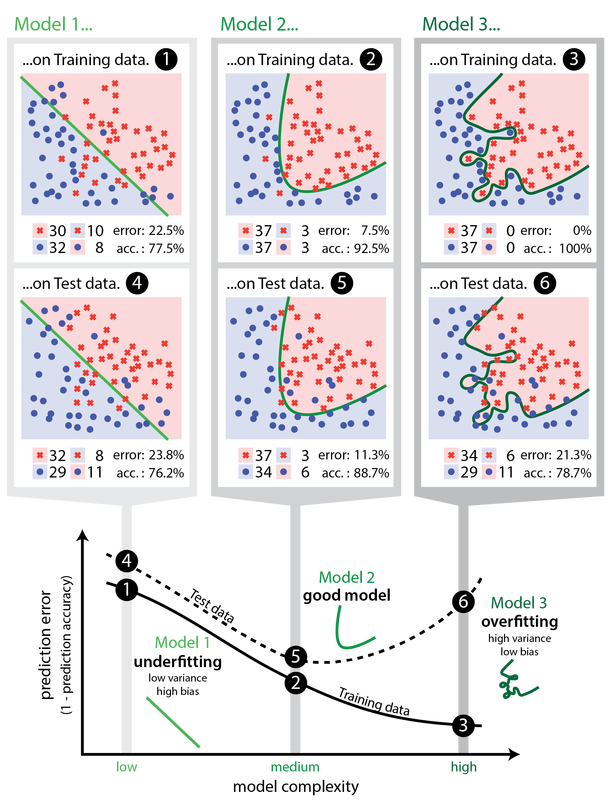
\includegraphics{images/unde_over_fitting.JPG}
\caption{\label{fig:unnamed-chunk-10}Przykłady niedoucznia (wykresy 1 i 4), poprawego modelu (2 i 5) i przeuczenia (3 i 6). Pierwszy wiersz wykresów pokazuje klasyfikację na podstawie modelu na zbiorze uczącym, a drugi na zbiorze testowym. Wykres na dole pokazuje związek pomiędzy złożonością modelu a wielkością błędu predykcji. \emph{Źródło}: \url{https://cambridgecoding.wordpress.com/2016/03/24/misleading-modelling-overfitting-cross-validation-and-the-bias-variance-trade-off/}}
\end{figure}

\hypertarget{modele-regresyjne}{%
\section{Modele regresyjne}\label{modele-regresyjne}}

Jednym z rodzajów zadań bazującym na wnioskowaniu indukcyjnym jest model regresyjny. Należy on do grupy metod nadzorowanych, których celem jest oszacowanie wartości cechy wyjściowej (która jest ilościowa) na podstawie zestawu predyktorów, które mogą być ilościowe i jakościowe. Uczenie takich modeli odbywa się poprzez optymalizację funkcji celu (np. \(MSE\)) na podstawie zbioru uczącego.

\hypertarget{modele-klasyfikacyjne}{%
\section{Modele klasyfikacyjne}\label{modele-klasyfikacyjne}}

Podobnie jak modele regresyjne, modele klasyfikacyjne należą do grupy metod nadzorowanego uczenia maszynowego. Ich zadaniem jest właściwa klasyfikacja obiektów na podstawie wielkości predyktorów. Odpowiedzią modelu jest zawsze cecha typu jakościowego, natomiast predyktory mogą mieć dowolny typ. Wyróżnia się klasyfikację dwu i wielostanową. Lista modeli realizujących klasyfikację binarną jest nieco dłuższa niż w przypadku modeli z wielostanową cechą wynikową. Proces uczenia modelu klasyfikacyjnego również opiera się na optymalizacji funkcji celu. Tym razem są to zupełnie inne miary jakości dopasowania (np. trafność, czyli odsetek poprawnych klasyfikacji).

\hypertarget{modele-grupujace}{%
\section{Modele grupujące}\label{modele-grupujace}}

Bardzo szeroką gamę modeli nienadzorowanych stanowią metody analizy skupień. Ich zadaniem jest grupowanie obiektów w możliwie najbardziej jednorodne grupy, na podstawie wartości atrybutów poddanych analizie. Ponieważ są to metody ``bez nauczyciela'', to ocena ich przydatności ma nieco inny charakter i choć istnieją różne wskaźniki jakości grupowania, to trudno tu o obiektywne wskazanie najlepszego rozwiązania.

\hypertarget{drzewa-decyzyjne}{%
\chapter{Drzewa decyzyjne}\label{drzewa-decyzyjne}}

\emph{Drzewo decyzyjne}\footnote{wyglądem przypomina odwrócone drzewo, stąd nazwa} jest strukturą hierarchiczną przedstawiającą model klasyfikacyjny lub regresyjny. Stosowane są szczególnie często wówczas, gdy funkcyjna postać związku pomiędzy predyktorami a zmienną wynikową jest nieznana lub ciężka do ustalenia.
Każde drzewo decyzyjne składa się z korzenia (ang. \emph{root}), węzłów (ang. \emph{nodes}) i liści (ang. \emph{leaves}). Korzeniem nazywamy początkowy węzeł drzewa, z którego poprzez podziały (ang. \emph{splits}) powstają kolejne węzły potomne. Końcowe węzły, które nie podlegają podziałom nazywamy liśćmi, a linie łączące węzły nazywamy gałęziami (ang. \emph{branches}).

Jeśli drzewo służy do zadań klasyfikacyjnych, to liście zawierają informację o tym, która klasa w danym ciągu podziałów jest najbardziej prawdopodobna. Natomiast, jeśli drzewo jest regresyjne, to liście zawierają warunkowe miary tendencji centralnej (najczęściej średnią) wartości zmiennej wynikowej. Warunek stanowi szereg podziałów doprowadzający do danego węzła terminalnego (liścia). W obu przypadkach (klasyfikacji i regresji) drzewo ``dąży'' do takiego podziału by kolejne węzły, a co za tym idzie również liście, były ja najbardziej jednorodne ze względu na zmienną wynikową.

\begin{figure}
\centering
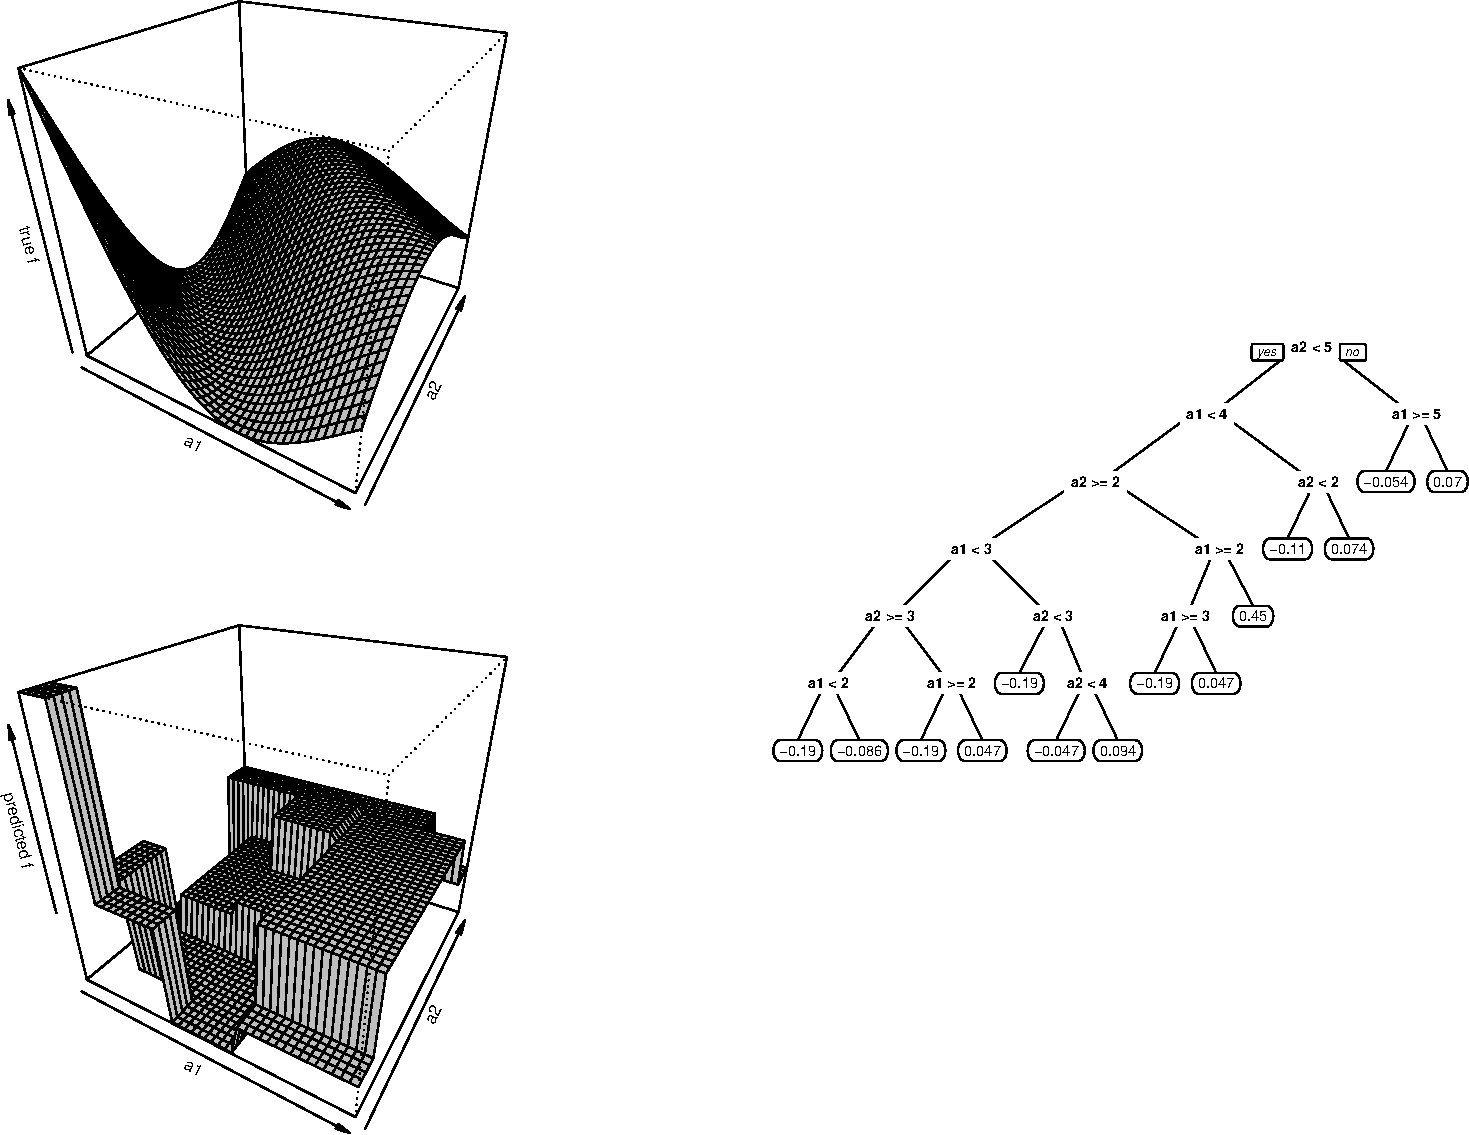
\includegraphics{EksploracjaDanych_files/figure-latex/unnamed-chunk-11-1.pdf}
\caption{\label{fig:unnamed-chunk-11}Przykład działania drzewa regresyjnego. Wykes w lewym górnym rogu pokazuje prawdziwą zależność, wyres po prawej stronie jest ilustracją drzewa decyzyjnego, a wykres w lewym dolnym rogu pokazuje dyskretyzację przestrzeni dokonaną przez drzewo, czyli sposób jego działania.}
\end{figure}

\hypertarget{wezy-i-gaezie}{%
\section{Węzły i gałęzie}\label{wezy-i-gaezie}}

Każdy podział rozdziela dziedzinę \(X\) na dwa lub więcej podobszarów dziedziny i wówczas każda obserwacja węzła nadrzędnego jest przyporządkowana węzłom potomnym. Każdy odchodzący węzeł potomny jest połączony gałęzią, która to wiąże się ściśle z możliwymi wynikami podziału. Każdy \(\mathbf{n}\)-ty węzeł można opisać jako podzbiór dziedziny w następujący sposób
\begin{equation}
    X_{\mathbf{n}}=\{x\in X|t_1(x)=r_1,t_2(x)=r_2,\ldots,t_k(x)=r_k\},
\end{equation}
gdzie \(t_1,t_2,\ldots,t_k\) są podziałami, które przeprowadzają \(x\) w obszary \(r_1, r_2,\ldots, r_k\). Przez
\begin{equation}
    S_{\mathbf{n}, t=r}=\{x\in S|t(x)=r\}
\end{equation}
rozumiemy, że dokonano takiego ciągu podziałów zbioru \(S\), że jego wartości znalazły się w \(\mathbf{n}\)-tym węźle.

\hypertarget{rodzaje-regu-podziau}{%
\section{Rodzaje reguł podziału}\label{rodzaje-regu-podziau}}

Najczęściej występujące reguły podziału w drzewach decyzyjnych są jednowymiarowe, czyli warunek podziału jest generowany na podstawie jednego atrybutu. Istnieją podziały wielowymiarowe ale ze względu na złożoność obliczeniową są rzadziej stosowane.

\hypertarget{podziay-dla-atrybutow-ze-skali-nominalnej}{%
\subsection{Podziały dla atrybutów ze skali nominalnej}\label{podziay-dla-atrybutow-ze-skali-nominalnej}}

Istnieją dwa typy reguł podziału dla skali nominalnej:

\begin{itemize}
\tightlist
\item
  oparte na wartości atrybutu (ang. \emph{value based}) - wówczas funkcja testowa przyjmuje postać \(t(x)=a(x)\), czyli podział generują wartości atrybutu;
\item
  oparte na równości (ang. \emph{equality based}) - gdzie funkcja testowa jest zdefiniowana jako
  \begin{equation}
    t(x)= \begin{cases}
        1, &\text{ gdy } a(x)=\nu\\
        0, & \text{ w przeciwnym przypadku},
    \end{cases}
  \end{equation}
  gdzie \(\nu\in A\) i \(A\) jest zbiorem możliwych wartości \(a\). W tym przypadku podział jest dychotomiczny, albo obiekt ma wartość atrybutu równą \(\nu\), albo go nie ma.
\end{itemize}

\hypertarget{podziay-dla-atrybutow-ze-skali-ciagej}{%
\subsection{Podziały dla atrybutów ze skali ciągłej}\label{podziay-dla-atrybutow-ze-skali-ciagej}}

Reguły podziału stosowane do skali ciągłej, to:

\begin{itemize}
\tightlist
\item
  oparta na nierównościach (ang. \emph{inequality based}) - zdefiniowana jako
  \begin{equation}
  t(x) = \begin{cases}
    1, &\text{ gdy }a(x)\leq \nu\\
    0, & \text{w przeciwnym przypadku},
    \end{cases}
  \end{equation}
  gdzie \(\nu\in A\);
\item
  przedziałowa (ang. \emph{interval based}) - zdefiniowana jako
  \begin{equation}
    t(x) = \begin{cases}
        1, &\text{ gdy }a(x) \in I_1\\
        2, &\text{ gdy }a(x) \in I_2\\
        \vdots & \\
        k, &\text{ gdy }a(x) \in I_k\\
    \end{cases}
  \end{equation}
  gdzie \(I_1,I_2,\ldots,I_k\subset A\) stanowią rozłączny podział (przedziałami) przeciwdziedziny \(A\).
\end{itemize}

\hypertarget{podziay-dla-atrybutow-ze-skali-porzadkowej}{%
\subsection{Podziały dla atrybutów ze skali porządkowej}\label{podziay-dla-atrybutow-ze-skali-porzadkowej}}

Podziały te mogą wykorzystywać oba wcześniej wspomniane typy, w zależności od potrzeb.

\hypertarget{algorytm-budowy-drzewa}{%
\section{Algorytm budowy drzewa}\label{algorytm-budowy-drzewa}}

\begin{enumerate}
\def\labelenumi{\arabic{enumi}.}
\tightlist
\item
  stwórz początkowy węzeł (korzeń) i oznacz go jako \emph{otwarty};
\item
  przypisz wszystkie możliwe rekordy do węzła początkowego;
\item
  \textbf{dopóki} istnieją otwarte węzły \textbf{wykonuj}:

  \begin{itemize}
  \tightlist
  \item
    wybierz węzeł \(\mathbf{n}\), wyznacz potrzebne statystyki opisowe zmiennej zależnej dla tego węzła i przypisz wartość docelową;
  \item
    \textbf{jeśli} kryterium zatrzymania podziału jest spełnione dla węzła \(n\), \textbf{to} oznacz go za \textbf{zamknięty};
  \item
    \textbf{w przeciwnym przypadku} wybierz podział \(r\) elementów węzła \(\mathbf{n}\), i dla każdego podzbioru podziału stwórz węzeł niższego rzędu (potomka) \(\mathbf{n}_r\) oraz oznacz go jako \emph{otwarty};
  \item
    następnie przypisz wszystkie przypadki generowane podziałem \(r\) do odpowiednich węzłów potomków \(\mathbf{n}_r\);
  \item
    oznacza węzeł \(\mathbf{n}\) jako \emph{zamknięty}.
  \end{itemize}
\end{enumerate}

Sposób przypisywania wartości docelowej wiąże się ściśle z rodzajem drzewa. W drzewach regresyjnych chodzi o wyliczenie średniej lub mediany dla obserwacji ujętych w danym węźle. Natomiast w przypadku drzewa klasyfikacyjnego, wyznacza się wartości prawdopodobieństw przynależności obserwacji znajdującej się w danym węźle do poszczególnych klas
\begin{equation}
    \P(d|\mathbf{n})=\P_{T_\mathbf{n}}(d)=\frac{|T_\mathbf{n}^d|}{|T_\mathbf{n}|},
\end{equation}
gdzie \(T_\mathbf{n}\) oznaczają obserwacje zbioru uczącego znajdujące się w węźle \(\mathbf{n}\), a \(T_\mathbf{n}^d\) oznacza dodatkowo podzbiór zbioru uczącego w \(\mathbf{n}\) węźle, które należą do klasy \(d\). Oczywiście klasyfikacja na podstawie otrzymanych prawdopodobieństw w danym węźle jest dokonana przez wybór klasy charakteryzującej się najwyższym prawdopodobieństwem.

\hypertarget{kryteria-zatrzymania}{%
\section{Kryteria zatrzymania}\label{kryteria-zatrzymania}}

Kryterium zatrzymania jest warunkiem, który decyduje o tym, że dany węzeł uznajemy za zamknięty i nie dokonujemy dalszego jego podziału. Wyróżniamy następujące kryteria zatrzymania:

\begin{itemize}
\tightlist
\item
  jednorodność węzła - w przypadku drzewa klasyfikacyjnego może zdarzyć się sytuacja, że wszystkie obserwacje węzła będą pochodziły z jednej klasy. Wówczas nie ma sensu dokonywać dalszego podziału węzła;
\item
  węzeł jest pusty - zbiór przypisanych obserwacji zbioru uczącego do \(\mathbf{n}\)-tego węzła jest pusty;
\item
  brak reguł podziału - wszystkie reguły podziału zostały wykorzystane, zatem nie da się stworzyć potomnych węzłów, które charakteryzowałyby się większą homogenicznością;
\end{itemize}

Warunki ujęte w pierwszych dwóch kryteriach mogą być nieco złagodzone, poprzez zatrzymanie podziałów wówczas, gdy prawdopodobieństwo przynależenia do pewnej klasy przekroczy ustalony próg lub gdy liczebność węzła spadnie poniżej ustalonej wartości.

W literaturze tematu istnieje jeszcze jedno często stosowane kryterium zatrzymania oparte na wielkości drzewa. Węzeł potomny ustala się jako zamknięty, gdy długość ścieżki dojścia do nie go przekroczy ustaloną wartość.

\hypertarget{reguy-podziau}{%
\section{Reguły podziału}\label{reguy-podziau}}

Ważnym elementem algorytmu tworzenia drzewa regresyjnego jest \emph{reguła podziału}. Dobierana jest w taki sposób aby zmaksymalizować zdolności generalizacyjne drzewa. Złożoność drzewa mierzona jest najczęściej przeciętną liczbą podziałów potrzebnych do dotarcia do liścia zaczynając od korzenia. Liście są najczęściej tworzone wówczas gdy dyspersja wartości wynikowej jest stosunkowo mała lub węzeł zawiera w miarę homogeniczne obserwacje ze względu na przynależność do klasy zmiennej wynikowej. W przypadku drzew regresyjnych zmienność na poziomie węzłów jest dobrą miarą służącą do definiowania podziału w węźle. I tak, jeśli pewien podział generuje nam stosunkowo małe dyspersje wartości docelowych w węzłach potomnych, to można ten podział uznać za właściwy. Jeśli \(T_n\) oznacza zbiór rekordów należących do węzła \(n\), a \(T_{n,t=r}\) są podzbiorami generowanymi przez podział \(r\) w węzłach potomnych dla \(n\), to dyspersję wartości docelowej \(f\) będziemy oznaczali następująco
\begin{equation}\label{dyspersja}
     \operatorname{disp}_{T_{n,t=r}}(f).
\end{equation}

Regułę podziału możemy określać poprzez minimalizację średniej ważonej dyspersji wartości docelowej następującej postaci
\begin{equation}\label{reg_podz}
        \operatorname{disp}_n(f|t)=\sum_{r\in R_t}\frac{|T_{n,t=r}|}{|T_n|}\operatorname{disp}_{T_{n,t=r}}(f),
\end{equation}
gdzie \(|\  |\) oznacza moc zbioru, a \(R_t\) zbiór wszystkich możliwych wartości reguły podziału. Czasami wygodniej będzie maksymalizować przyrost dyspersji (lub spadek)
\begin{equation}\label{przyrost}
        \bigtriangleup \operatorname{disp}_n(f|t)=\operatorname{disp}_n(f)-\sum_{r\in R_t}\frac{|T_{n,t=r}|}{|T_n|}\operatorname{disp}_{T_{n,t=r}}(f).
\end{equation}

Miarą heterogeniczności węzłów ze względu na zmienną wynikową (ang. \emph{impurity}) w drzewach klasyfikacyjnych, która pozwala na tworzenie kolejnych podziałów węzła, są najczęściej wskaźnik Gini'ego i entropia (Breiman \protect\hyperlink{ref-breiman1998}{1998}).

Entropią podzbioru uczącego w węźle \(\mathbf{n}\), wyznaczamy wg wzoru
\begin{equation}
E_{T_{\mathbf{n}}}(c|t) = \sum_{x\in R_t} \frac{|T_{\mathbf{n}, t=r}|}{|T_{\mathbf{n}}|}E_{T_{\mathbf{n}, t=r}}(c),
\end{equation}
gdzie \(t\) jest podziałem (kandydatem), \(r\) potencjalnym wynikiem podziału \(t\), \(c\) jest oznaczeniem klasy zmiennej wynikowej, a
\begin{equation}
    E_{T_{\mathbf{n}, t=r}}(c) = \sum_{d\in C}-\P_{T_{\mathbf{n}, t=r}}(c=d)\log\P_{T_{\mathbf{n}, t=r}}(c=d),
\end{equation}
przy czym
\begin{equation}
    \P_{T_{\mathbf{n}, t=r}}(c=d)= \P_{T_{\mathbf{n}}}(c=d|t=r).
\end{equation}

Podobnie definiuje się indeks Gini'ego
\begin{equation}
Gi_{T_{\mathbf{n}}}(c|t) = \sum_{x\in R_t} \frac{|T_{\mathbf{n}, t=r}|}{|T_{\mathbf{n}}|}Gi_{T_{\mathbf{n}, t=r}}(c),
\end{equation}
gdzie
\begin{equation}
    Gi_{T_{\mathbf{n}, t=r}}(c) = \sum_{d\in C}\P_{T_{\mathbf{n}, t=r}}(c=d)\cdot(1-\P_{T_{\mathbf{n}, t=r}}(c=d))= 1-\sum_{d\in C}\P^2_{T_{\mathbf{n}, t=r}}(c=d).
\end{equation}
Dla tak zdefiniowanych miar ``nieczystości'' węzłów, podziału dokonujemy w taki sposób, aby zminimalizować współczynnik Gini'ego lub entropię. Im niższe miary nieczystości, tym bardziej obserwacje znajdujące się w węźle są monokulturą\footnote{prawie wszystkie są w jednej klasie}. Nierzadko korzysta się również z współczynnika przyrostu informacji (ang. \emph{information gain})
\begin{equation}
    \Delta E_{T_{\mathbf{n}}}(c|t)=E_{T_{\mathbf{n}}}(c)-E_{T_{\mathbf{n}}}(c|t).
\end{equation}
Istnieje również jego odpowiednik dla indeksu Gini'ego. W obu przypadkach optymalnego podziału szukamy poprzez maksymalizację przyrostu informacji.

\hypertarget{przycinanie-drzewa-decyzyjnego}{%
\section{Przycinanie drzewa decyzyjnego}\label{przycinanie-drzewa-decyzyjnego}}

Uczenie drzewa decyzyjnego wiąże się z ryzykiem przeuczenia modelu (podobnie jak to się ma w przypadku innych modeli predykcyjnych). Wcześniej przytoczone reguły zatrzymania (np. głębokość drzewa czy zatrzymanie przy osiągnięciu jednorodności na zadanym poziomie) pomagają kontrolować poziom generalizacji drzewa ale czasami będzie dodatkowo potrzebne przycięcie drzewa, czyli usunięcie pewnych podziałów, a co za tym idzie, również liści (węzłów).

\hypertarget{przycinanie-redukujace-bad}{%
\subsection{Przycinanie redukujące błąd}\label{przycinanie-redukujace-bad}}

Jedną ze strategii przycinania drzewa jest przycinanie redukujące błąd (ang. \emph{reduced error pruning}). Polega ono na porównaniu błędów (najczęściej używana jest miara odsetka błędnych klasyfikacji lub MSE) liścia \(\mathbf{l}\) i węzła do którego drzewo przycinamy \(\mathbf{n}\) na całkiem nowym zbiorze uczącym \(R\). Niech \(e_R(\mathbf{l})\) i \(e_R(\mathbf{n})\) oznaczają odpowiednio błędy na zbiorze \(R\) liścia i węzła. Przez błąd węzła rozumiemy błąd pod-drzewa o korzeniu \(\mathbf{n}\). Wówczas jeśli zachodzi warunek
\begin{equation}
    e_R(\mathbf{l})\leq e_R(\mathbf{n}), 
\end{equation}
to zaleca się zastąpić węzeł \(\mathbf{n}\) liściem \(\mathbf{l}\).

\hypertarget{przycinanie-minimalizujace-bad}{%
\subsection{Przycinanie minimalizujące błąd}\label{przycinanie-minimalizujace-bad}}

Przycinanie minimalizujące błąd opiera się na spostrzeżeniu, że błąd drzewa przyciętego charakteryzuje się zbyt pesymistyczną oceną i dlatego wymaga korekty. Węzeł drzewa klasyfikacyjnego \(\mathbf{n}\) zastępujemy liściem \(\mathbf{l}\), jeśli
\begin{equation}
    \hat{e}_T(\mathbf{l})\leq \hat{e}_T(\mathbf{n}),
\end{equation}
gdzie
\begin{equation}
    \hat{e}_T(\mathbf{n})=\sum_{\mathbf{n}'\in N(\mathbf{n})}\frac{|T_{\mathbf{n}'}|}{|T_\mathbf{n}|}\hat{e}_T(\mathbf{n}'),
\end{equation}
a \(N(\mathbf{n})\) jest zbiorem wszystkich możliwych węzłów potomnych węzła \(\mathbf{n}\) i \begin{equation}
    \hat{e}_T(\mathbf{l})=1-\frac{|\{x\in T_\mathbf{l}|c(x)=d_{\mathbf{l}}\}|+mp}{|T_\mathbf{l}|+m},
\end{equation}
gdzie \(p\) jest prawdopodobieństwem przynależności do klasy \(d_{\mathbf{l}}\) ustalona na podstawie zewnętrznej wiedzy (gdy jej nie posiadamy przyjmujemy \(p=1/|C|\)).

W przypadku drzewa regresyjnego znajdujemy wiele analogii, ponieważ jeśli dla pewnego zbioru rekordów \(T\) spełniony jest warunek
\begin{equation}\label{kryterium1}
    \operatorname{mse}_T(\mathbf{l})\leq\operatorname{mse}_T(\mathbf{n}),
\end{equation}
gdzie \(\mathbf{l}\) i \(\mathbf{n}\) oznaczają odpowiednio liść i węzeł, to wówczas zastępujemy węzeł \(\mathbf{n}\) przez liść \(\mathbf{l}\).

Estymatory wyznaczone na podstawie niewielkiej próby, mogą być obarczone znaczącym błędem. Wyliczanie błędu średnio-kwadratowego dla podzbioru nowych wartości może się charakteryzować takim obciążeniem. Dlatego stosuje się statystyki opisowe z poprawką, której pochodzenie może mieć trzy źródła: wiedza merytoryczna na temat szukanej wartości, założeń modelu lub na podstawie wyliczeń opartych o cały zbiór wartości.

Skorygowany estymator błędu średnio-kwadratowego ma następującą postać
\begin{equation}\label{mse}
        \widehat{\operatorname{mse}}_T(\mathbf{l})=\frac{\sum_{x\in T}(f(x)-m_{\mathbf{l},m,m_0}(f))^2+mS_0^2}{|T_\mathbf{l}|+m},
\end{equation}
gdzie
\begin{equation}\label{poprawka}
        m_{\mathbf{l},m,m_0}(f)=\frac{\sum_{x\in T_\mathbf{l}}f(x)+mm_0}{|T_\mathbf{l}|+m},
\end{equation}
a \(m_0\) i \(S_0^2\) są średnią i wariancją wyznaczonymi na całej próbie uczącej.
Błąd średnio-kwadratowy węzła \(\mathbf{n}\) ma postać
\begin{equation}\label{propagacja}
        \widehat{\operatorname{mse}}_T(\mathbf{n})=\sum_{\mathbf{n}'\in N(\mathbf{n})}\frac{|T_{\mathbf{n}'}|}{|T_\mathbf{n}|}\widehat{\operatorname{mse}}_T(\mathbf{n}').
\end{equation}
Wówczas kryterium podcięcia można zapisać w następujący sposób
\begin{equation}\label{kryterium2}
        \widehat{\operatorname{mse}}_T(\mathbf{l}) \leq \widehat{\operatorname{mse}}_T(\mathbf{n})
\end{equation}

\hypertarget{przycinanie-ze-wzgledu-na-wspoczynnik-zozonosci-drzewa}{%
\subsection{Przycinanie ze względu na współczynnik złożoności drzewa}\label{przycinanie-ze-wzgledu-na-wspoczynnik-zozonosci-drzewa}}

Przycinanie ze względu na współczynnik złożoności drzewa (ang. \emph{cost-complexity pruning}) polega na wprowadzeniu ``kary'' za zwiększoną złożoność drzewa. Drzewa klasyfikacyjne przycinamy gdy spełniony jest warunek
\begin{equation}
    e_T(\mathbf{l})\leq e_T(\mathbf{n})+\alpha C(\mathbf{n}),
\end{equation}
gdzie \(C(\mathbf{n})\) oznacza złożoność drzewa mierzoną liczbą liści, a \(\alpha\) parametrem wagi kary za złożoność drzewa.

Wspomniane kryterium przycięcia dla drzew regresyjnych bazuje na względnym błędzie średnio-kwadratowym (ang. \emph{relative square error}), czyli
\begin{equation}\label{rse}
        \widehat{\operatorname{rse}}_T(\mathbf{n})=\frac{|T|\widehat{\operatorname{mse}}_T(\mathbf{n})}{(|T|-1)S^2_T(f)},
\end{equation}
gdzie \(T\) oznacza podzbiór \(X\), \(S^2_T\) wariancję na zbiorze \(T\).
Wówczas kryterium podcięcia wygląda następująco
\begin{equation}\label{kryterium3}
    \widehat{\operatorname{rse}}_T(\mathbf{l})\leq \widehat{\operatorname{rse}}_T(\mathbf{n})+\alpha C(\mathbf{n}).
\end{equation}

\hypertarget{obsuga-brakow-danych}{%
\section{Obsługa braków danych}\label{obsuga-brakow-danych}}

Drzewa decyzyjne wyjątkowo dobrze radzą sobie z obsługa zbiorów z brakami. Stosowane są głównie dwie strategie:

\begin{itemize}
\tightlist
\item
  udziałów obserwacji (ang. \emph{fractional instances}) - rozważane są wszystkie możliwe podziały dla brakującej obserwacji i przypisywana jest im odpowiednia waga lub prawdopodobieństwo, w oparciu o zaobserwowany rozkład znanych obserwacji. Te same wagi są stosowane do predykcji wartości na podstawie drzewa z brakami danych.
\item
  podziałów zastępczych (ang. \emph{surrogate splits}) - jeśli wynik podziału nie może być ustalony dla obserwacji z brakami, to używany jest podział zastępczy (pierwszy), jeśli i ten nie może zostać ustalony, to stosuje się kolejny. Kolejne podziały zastępcze są generowane tak, aby wynik podziału możliwie najbardziej przypominał podział właściwy.
\end{itemize}

\hypertarget{zalety-i-wady}{%
\section{Zalety i wady}\label{zalety-i-wady}}

\hypertarget{zalety}{%
\subsection{Zalety}\label{zalety}}

\begin{itemize}
\tightlist
\item
  łatwe w interpretacji;
\item
  nie wymagają żmudnego przygotowania danych (brak standaryzacji, wprowadzania zmiennych binarnych, dopuszcza występowanie braków danych);
\item
  działa na obu typach zmiennych - jakościowych i ilościowych;
\item
  dopuszcza nieliniowość związku między zmienną wynikową a predyktorami;
\item
  odporny na odstępstwa od założeń;
\item
  pozwala na obsługę dużych zbiorów danych.
\end{itemize}

\hypertarget{wady}{%
\subsection{Wady}\label{wady}}

\begin{itemize}
\tightlist
\item
  brak jawnej postaci zależności;
\item
  zależność struktury drzewa od użytego algorytmu;
\item
  przegrywa jakością predykcji z innymi metodami nadzorowanego uczenia maszynowego.
\end{itemize}

\BeginKnitrBlock{example}
\protect\hypertarget{exm:przyk41}{}{\label{exm:przyk41} }Przykładem zastosowania drzew decyzyjnych będzie klasyfikacja irysów na podstawie długości i szerokości kielicha i płatka.
\EndKnitrBlock{example}

Przykładem zastosowania drzew decyzyjnych będzie klasyfikacja irysów na podstawie długości i szerokości kielicha i płatka.

\begin{Shaded}
\begin{Highlighting}[]
\KeywordTok{library}\NormalTok{(tidyverse) }
\KeywordTok{library}\NormalTok{(rpart) }\CommentTok{# pakiet do tworzenia drzew typu CART}
\KeywordTok{library}\NormalTok{(rpart.plot) }\CommentTok{# pakiet do rysowania drzew}
\end{Highlighting}
\end{Shaded}

Każde zadanie ucznia maszynowego zaczynamy od czyszczenia danych i odpowiedniego ich przygotowania ale w tym przypadku skupimy się jedynie na budowie, optymalizacji i ewaluacji modelu.

\textbf{Podział zbioru na próbę uczącą i testową}

\begin{Shaded}
\begin{Highlighting}[]
\KeywordTok{set.seed}\NormalTok{(}\DecValTok{44}\NormalTok{)}
\NormalTok{dt.train <-}\StringTok{ }\NormalTok{iris }\OperatorTok\StringTok{ }
\StringTok{    }\KeywordTok{sample_frac}\NormalTok{(}\DataTypeTok{size =} \FloatTok{0.7}\NormalTok{)}
\NormalTok{dt.test <-}\StringTok{ }\KeywordTok{setdiff}\NormalTok{(iris, dt.train)}
\KeywordTok{str}\NormalTok{(dt.train)}
\end{Highlighting}
\end{Shaded}

\begin{verbatim}
## 'data.frame':    105 obs. of  5 variables:
##  $ Sepal.Length: num  6.4 4.4 6.6 5.4 5 5.4 5.6 4.4 5.4 6.1 ...
##  $ Sepal.Width : num  2.7 3.2 3 3 3.6 3.4 2.9 2.9 3.9 2.9 ...
##  $ Petal.Length: num  5.3 1.3 4.4 4.5 1.4 1.7 3.6 1.4 1.3 4.7 ...
##  $ Petal.Width : num  1.9 0.2 1.4 1.5 0.2 0.2 1.3 0.2 0.4 1.4 ...
##  $ Species     : Factor w/ 3 levels "setosa","versicolor",..: 3 1 2 2 1 1 2 1 1 2 ...
\end{verbatim}

\begin{Shaded}
\begin{Highlighting}[]
\KeywordTok{str}\NormalTok{(dt.test)}
\end{Highlighting}
\end{Shaded}

\begin{verbatim}
## 'data.frame':    45 obs. of  5 variables:
##  $ Sepal.Length: num  4.7 4.6 5.4 4.8 5.8 5.1 5.1 5.1 5 5.2 ...
##  $ Sepal.Width : num  3.2 3.1 3.9 3.4 4 3.8 3.7 3.3 3 3.5 ...
##  $ Petal.Length: num  1.3 1.5 1.7 1.6 1.2 1.5 1.5 1.7 1.6 1.5 ...
##  $ Petal.Width : num  0.2 0.2 0.4 0.2 0.2 0.3 0.4 0.5 0.2 0.2 ...
##  $ Species     : Factor w/ 3 levels "setosa","versicolor",..: 1 1 1 1 1 1 1 1 1 1 ...
\end{verbatim}

\textbf{Budowa drzewa}

Budowy drzewa dokonujemy za pomocą funkcji \texttt{rpart} pakietu \textbf{rpart} (Therneau and Atkinson \protect\hyperlink{ref-R-rpart}{2018}) stosując zapis formuły zależności. Drzewo zostanie zbudowane z uwzględnieniem kilku kryteriów zatrzymania:

\begin{itemize}
\tightlist
\item
  minimalna liczebność węzła, który może zostać podzielony to 10 - ze względu na małą liczebność zbioru uczącego;
\item
  minimalna liczebność liścia to 5 - aby nie dopuścić do przeuczenia modelu;
\item
  maksymalna głębokość drzewa to 4 - aby nie dopuścić do przeuczenia modelu.
\end{itemize}

\begin{Shaded}
\begin{Highlighting}[]
\NormalTok{mod.rpart <-}\StringTok{ }\KeywordTok{rpart}\NormalTok{(Species}\OperatorTok{~}\NormalTok{., }\DataTypeTok{data =}\NormalTok{ dt.train, }
                   \DataTypeTok{control =} \KeywordTok{rpart.control}\NormalTok{(}\DataTypeTok{minsplit =} \DecValTok{10}\NormalTok{,}
                                           \DataTypeTok{minbucket =} \DecValTok{5}\NormalTok{,}
                                           \DataTypeTok{maxdepth =} \DecValTok{4}\NormalTok{))}
\KeywordTok{summary}\NormalTok{(mod.rpart)}
\end{Highlighting}
\end{Shaded}

\begin{verbatim}
## Call:
## rpart(formula = Species ~ ., data = dt.train, control = rpart.control(minsplit = 10, 
##     minbucket = 5, maxdepth = 4))
##   n= 105 
## 
##           CP nsplit  rel error    xerror       xstd
## 1 0.51470588      0 1.00000000 1.1764706 0.06418173
## 2 0.41176471      1 0.48529412 0.6617647 0.07457243
## 3 0.02941176      2 0.07352941 0.1029412 0.03758880
## 4 0.01000000      3 0.04411765 0.1029412 0.03758880
## 
## Variable importance
##  Petal.Width Petal.Length Sepal.Length  Sepal.Width 
##           35           33           21           12 
## 
## Node number 1: 105 observations,    complexity param=0.5147059
##   predicted class=setosa      expected loss=0.647619  P(node) =1
##     class counts:    37    33    35
##    probabilities: 0.352 0.314 0.333 
##   left son=2 (37 obs) right son=3 (68 obs)
##   Primary splits:
##       Petal.Length < 2.45 to the left,  improve=35.95322, (0 missing)
##       Petal.Width  < 0.8  to the left,  improve=35.95322, (0 missing)
##       Sepal.Length < 5.45 to the left,  improve=25.39467, (0 missing)
##       Sepal.Width  < 3.35 to the right, improve=12.69596, (0 missing)
##   Surrogate splits:
##       Petal.Width  < 0.8  to the left,  agree=1.000, adj=1.000, (0 split)
##       Sepal.Length < 5.45 to the left,  agree=0.924, adj=0.784, (0 split)
##       Sepal.Width  < 3.35 to the right, agree=0.819, adj=0.486, (0 split)
## 
## Node number 2: 37 observations
##   predicted class=setosa      expected loss=0  P(node) =0.352381
##     class counts:    37     0     0
##    probabilities: 1.000 0.000 0.000 
## 
## Node number 3: 68 observations,    complexity param=0.4117647
##   predicted class=virginica   expected loss=0.4852941  P(node) =0.647619
##     class counts:     0    33    35
##    probabilities: 0.000 0.485 0.515 
##   left son=6 (38 obs) right son=7 (30 obs)
##   Primary splits:
##       Petal.Width  < 1.75 to the left,  improve=25.286380, (0 missing)
##       Petal.Length < 4.75 to the left,  improve=24.879360, (0 missing)
##       Sepal.Length < 5.75 to the left,  improve= 6.713875, (0 missing)
##       Sepal.Width  < 3.25 to the left,  improve= 1.336180, (0 missing)
##   Surrogate splits:
##       Petal.Length < 4.75 to the left,  agree=0.882, adj=0.733, (0 split)
##       Sepal.Length < 6.15 to the left,  agree=0.721, adj=0.367, (0 split)
##       Sepal.Width  < 3.15 to the left,  agree=0.618, adj=0.133, (0 split)
## 
## Node number 6: 38 observations,    complexity param=0.02941176
##   predicted class=versicolor  expected loss=0.1315789  P(node) =0.3619048
##     class counts:     0    33     5
##    probabilities: 0.000 0.868 0.132 
##   left son=12 (32 obs) right son=13 (6 obs)
##   Primary splits:
##       Petal.Length < 4.95 to the left,  improve=4.0800440, (0 missing)
##       Petal.Width  < 1.45 to the left,  improve=1.2257490, (0 missing)
##       Sepal.Width  < 2.65 to the right, improve=0.6168705, (0 missing)
##       Sepal.Length < 5.95 to the left,  improve=0.4736842, (0 missing)
##   Surrogate splits:
##       Petal.Width < 1.55 to the left,  agree=0.868, adj=0.167, (0 split)
## 
## Node number 7: 30 observations
##   predicted class=virginica   expected loss=0  P(node) =0.2857143
##     class counts:     0     0    30
##    probabilities: 0.000 0.000 1.000 
## 
## Node number 12: 32 observations
##   predicted class=versicolor  expected loss=0.03125  P(node) =0.3047619
##     class counts:     0    31     1
##    probabilities: 0.000 0.969 0.031 
## 
## Node number 13: 6 observations
##   predicted class=virginica   expected loss=0.3333333  P(node) =0.05714286
##     class counts:     0     2     4
##    probabilities: 0.000 0.333 0.667
\end{verbatim}

\begin{Shaded}
\begin{Highlighting}[]
\KeywordTok{rpart.plot}\NormalTok{(mod.rpart)}
\end{Highlighting}
\end{Shaded}

\begin{figure}
\centering
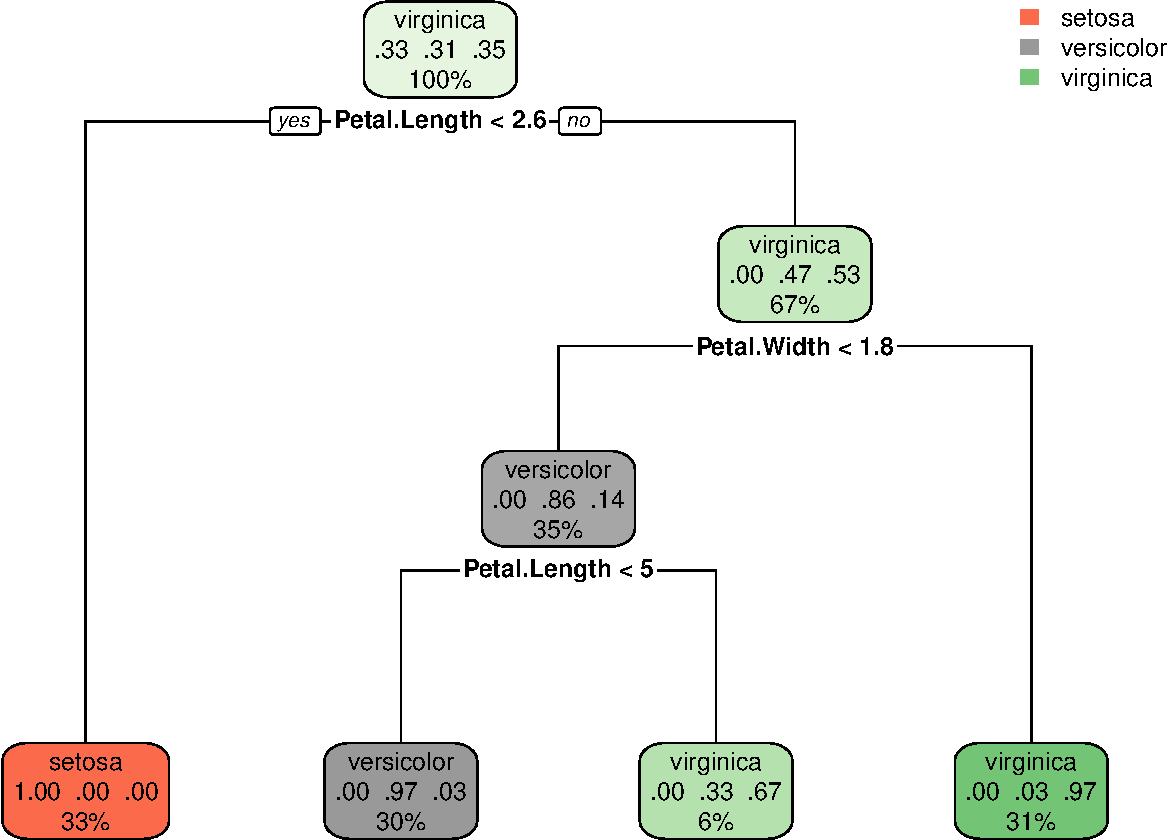
\includegraphics{EksploracjaDanych_files/figure-latex/unnamed-chunk-15-1.pdf}
\caption{\label{fig:unnamed-chunk-15}Obraz drzewa klasyfikacyjnego.}
\end{figure}

Powyższy wykres przedstawia strukturę drzewa klasyfikacyjnego. Kolorami są oznaczone klasy, które w danym węźle dominują. Nasycenie barwy decyduje o sile tej dominacji. W każdym węźle podana jest klasa, do której najprawdopodobniej należą jego obserwacje. Ponadto podane są proporcje przynależności do klas zmiennej wynikowej oraz procent obserwacji zbioru uczącego należących do danego węzła. Pod każdym węzłem podana jest reguła podziału.

\textbf{Przycinanie drzewa}

Zanim przystąpimy do przycinania drzewa należy sprawdzić, jakie są zdolności generalizacyjne modelu. Oceny tej dokonujemy najczęściej sprawdzając macierz klasyfikacji.

\begin{Shaded}
\begin{Highlighting}[]
\NormalTok{pred.prob <-}\StringTok{ }\KeywordTok{predict}\NormalTok{(mod.rpart, }
                     \DataTypeTok{newdata =}\NormalTok{ dt.test)}
\NormalTok{pred.prob[}\DecValTok{10}\OperatorTok{:}\DecValTok{20}\NormalTok{,]}
\end{Highlighting}
\end{Shaded}

\begin{verbatim}
##    setosa versicolor virginica
## 10      1    0.00000   0.00000
## 11      1    0.00000   0.00000
## 12      1    0.00000   0.00000
## 13      1    0.00000   0.00000
## 14      0    0.96875   0.03125
## 15      0    0.96875   0.03125
## 16      0    0.96875   0.03125
## 17      0    0.96875   0.03125
## 18      0    0.96875   0.03125
## 19      0    0.96875   0.03125
## 20      0    0.00000   1.00000
\end{verbatim}

\begin{Shaded}
\begin{Highlighting}[]
\NormalTok{pred.class <-}\StringTok{ }\KeywordTok{predict}\NormalTok{(mod.rpart, }
                      \DataTypeTok{newdata =}\NormalTok{ dt.test,}
                      \DataTypeTok{type =} \StringTok{"class"}\NormalTok{)}
\NormalTok{pred.class}
\end{Highlighting}
\end{Shaded}

\begin{verbatim}
##          1          2          3          4          5          6 
##     setosa     setosa     setosa     setosa     setosa     setosa 
##          7          8          9         10         11         12 
##     setosa     setosa     setosa     setosa     setosa     setosa 
##         13         14         15         16         17         18 
##     setosa versicolor versicolor versicolor versicolor versicolor 
##         19         20         21         22         23         24 
## versicolor  virginica versicolor versicolor versicolor versicolor 
##         25         26         27         28         29         30 
## versicolor versicolor versicolor versicolor versicolor versicolor 
##         31         32         33         34         35         36 
##  virginica  virginica  virginica  virginica  virginica  virginica 
##         37         38         39         40         41         42 
##  virginica  virginica  virginica  virginica  virginica  virginica 
##         43         44         45 
##  virginica  virginica  virginica 
## Levels: setosa versicolor virginica
\end{verbatim}

\begin{Shaded}
\begin{Highlighting}[]
\NormalTok{tab <-}\StringTok{ }\KeywordTok{table}\NormalTok{(}\DataTypeTok{predykcja =}\NormalTok{ pred.class, }\DataTypeTok{obserwacja =}\NormalTok{ dt.test}\OperatorTok{$}\NormalTok{Species)}
\NormalTok{tab}
\end{Highlighting}
\end{Shaded}

\begin{verbatim}
##             obserwacja
## predykcja    setosa versicolor virginica
##   setosa         13          0         0
##   versicolor      0         16         0
##   virginica       0          1        15
\end{verbatim}

Jak widać z powyższej tabeli, model całkiem dobrze radzi sobie z poprawną klasyfikacją obserwacji do odpowiednich kategorii. Tylko jedna obserwacja została błędnie zaklasyfikowana.

W dalszej kolejności sprawdzimy, czy nie jest konieczne przycięcie drzewa. Jednym z kryteriów przycinania drzewa jest przycinanie ze względu na złożoność drzewa. W tym przypadku jest wyrażony parametrem \texttt{cp}. Istnieje powszechnie stosowana reguła jednego odchylenia standardowego, która mówi, że drzewo należy przyciąć wówczas, gdy błąd oszacowany na podstawie sprawdzianu krzyżowego (\texttt{xerror}), pierwszy raz zejdzie poniżej poziomu wyznaczonego przez najniższą wartość błędu powiększonego o odchylenie standardowe tego błędu (\texttt{xstd}). Na podstawie poniższej tabeli można ustalić, że poziomem odcięcia jest wartość \(0.10294+0.037589=0.140529\). Pierwszy raz błąd przyjmuje wartość mniejszą od \(0.140529\) po drugim podziale (\texttt{nsplit=2}). Temu poziomowi odpowiada \texttt{cp} o wartości \(0.029412\) i to jest złożoność drzewa, którą powinniśmy przyjąć do przycięcia drzewa.

\begin{Shaded}
\begin{Highlighting}[]
\KeywordTok{printcp}\NormalTok{(mod.rpart)}
\end{Highlighting}
\end{Shaded}

\begin{verbatim}
## 
## Classification tree:
## rpart(formula = Species ~ ., data = dt.train, control = rpart.control(minsplit = 10, 
##     minbucket = 5, maxdepth = 4))
## 
## Variables actually used in tree construction:
## [1] Petal.Length Petal.Width 
## 
## Root node error: 68/105 = 0.64762
## 
## n= 105 
## 
##         CP nsplit rel error  xerror     xstd
## 1 0.514706      0  1.000000 1.17647 0.064182
## 2 0.411765      1  0.485294 0.66176 0.074572
## 3 0.029412      2  0.073529 0.10294 0.037589
## 4 0.010000      3  0.044118 0.10294 0.037589
\end{verbatim}

\begin{Shaded}
\begin{Highlighting}[]
\KeywordTok{plotcp}\NormalTok{(mod.rpart)}
\end{Highlighting}
\end{Shaded}

\begin{figure}
\centering
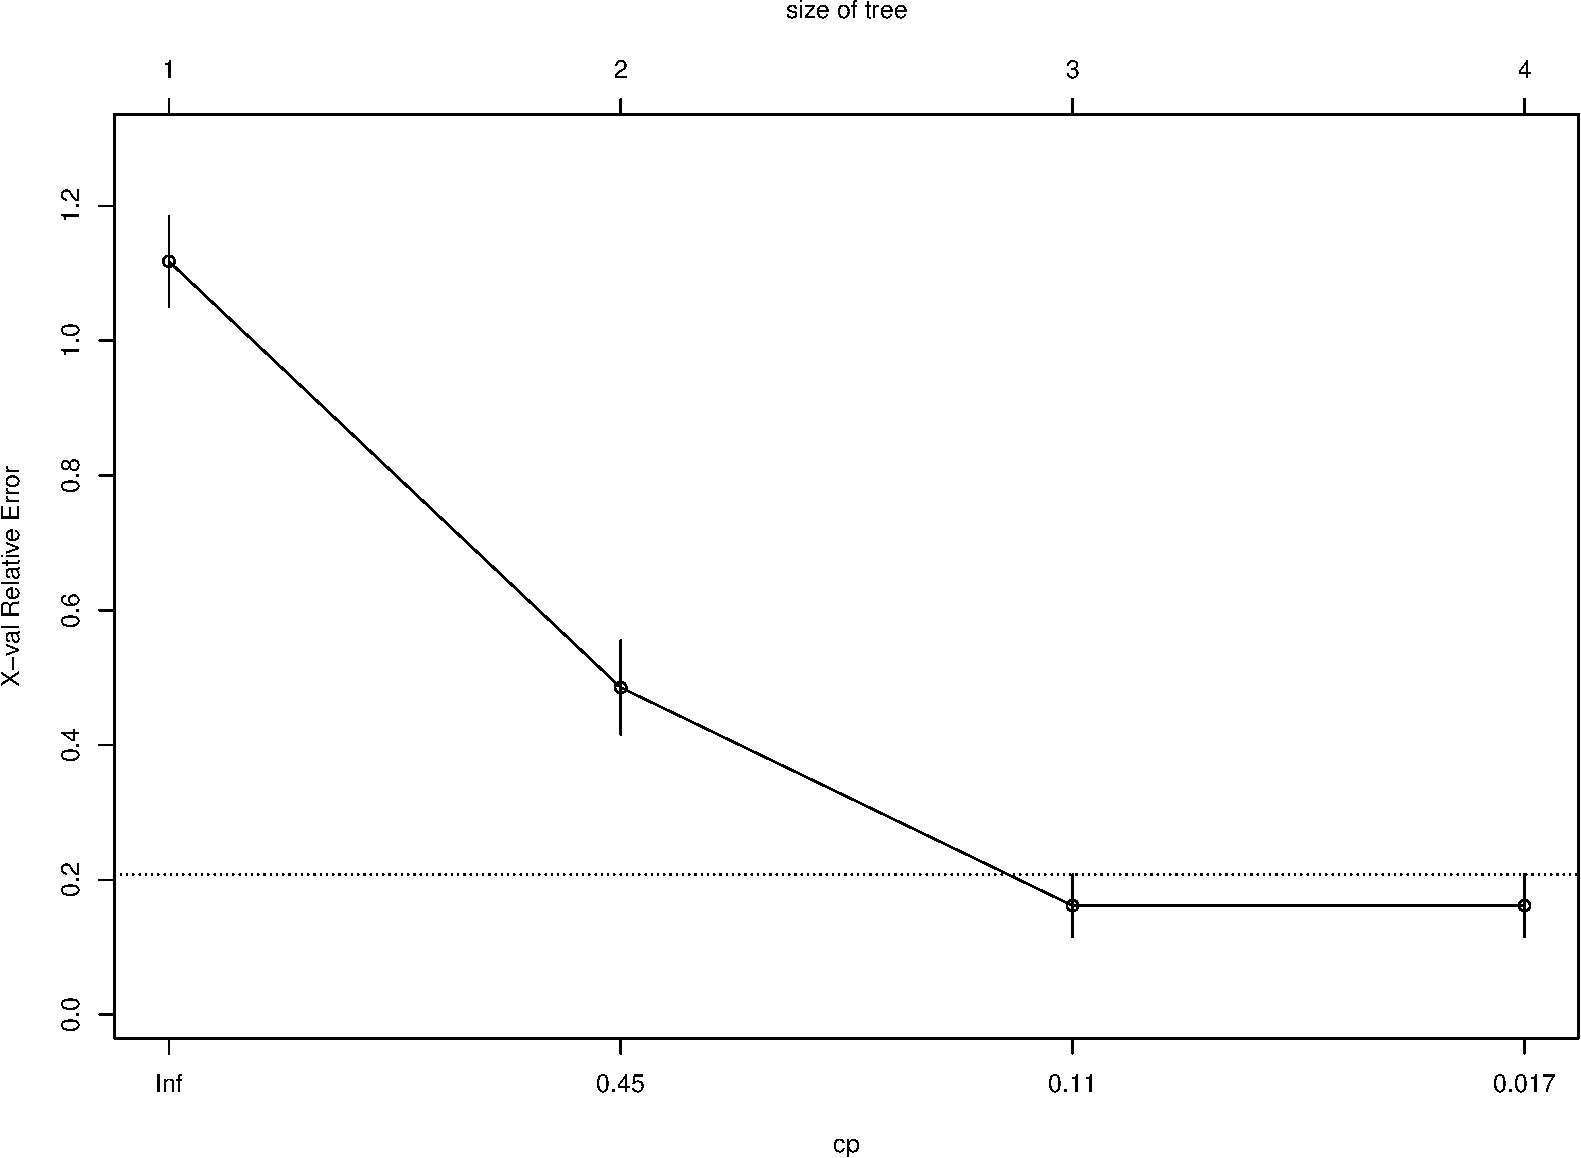
\includegraphics{EksploracjaDanych_files/figure-latex/unnamed-chunk-17-1.pdf}
\caption{\label{fig:unnamed-chunk-17}Na wykresie błędów punkt odcięcia zaznaczony jest linią przerywaną}
\end{figure}

Przycięte drzewo wygląda następująco:

\begin{Shaded}
\begin{Highlighting}[]
\NormalTok{mod.rpart2 <-}\StringTok{ }\KeywordTok{prune}\NormalTok{(mod.rpart, }\DataTypeTok{cp =} \FloatTok{0.029412}\NormalTok{)}
\KeywordTok{summary}\NormalTok{(mod.rpart2)}
\end{Highlighting}
\end{Shaded}

\begin{verbatim}
## Call:
## rpart(formula = Species ~ ., data = dt.train, control = rpart.control(minsplit = 10, 
##     minbucket = 5, maxdepth = 4))
##   n= 105 
## 
##          CP nsplit  rel error    xerror       xstd
## 1 0.5147059      0 1.00000000 1.1764706 0.06418173
## 2 0.4117647      1 0.48529412 0.6617647 0.07457243
## 3 0.0294120      2 0.07352941 0.1029412 0.03758880
## 
## Variable importance
##  Petal.Width Petal.Length Sepal.Length  Sepal.Width 
##           35           31           22           12 
## 
## Node number 1: 105 observations,    complexity param=0.5147059
##   predicted class=setosa      expected loss=0.647619  P(node) =1
##     class counts:    37    33    35
##    probabilities: 0.352 0.314 0.333 
##   left son=2 (37 obs) right son=3 (68 obs)
##   Primary splits:
##       Petal.Length < 2.45 to the left,  improve=35.95322, (0 missing)
##       Petal.Width  < 0.8  to the left,  improve=35.95322, (0 missing)
##       Sepal.Length < 5.45 to the left,  improve=25.39467, (0 missing)
##       Sepal.Width  < 3.35 to the right, improve=12.69596, (0 missing)
##   Surrogate splits:
##       Petal.Width  < 0.8  to the left,  agree=1.000, adj=1.000, (0 split)
##       Sepal.Length < 5.45 to the left,  agree=0.924, adj=0.784, (0 split)
##       Sepal.Width  < 3.35 to the right, agree=0.819, adj=0.486, (0 split)
## 
## Node number 2: 37 observations
##   predicted class=setosa      expected loss=0  P(node) =0.352381
##     class counts:    37     0     0
##    probabilities: 1.000 0.000 0.000 
## 
## Node number 3: 68 observations,    complexity param=0.4117647
##   predicted class=virginica   expected loss=0.4852941  P(node) =0.647619
##     class counts:     0    33    35
##    probabilities: 0.000 0.485 0.515 
##   left son=6 (38 obs) right son=7 (30 obs)
##   Primary splits:
##       Petal.Width  < 1.75 to the left,  improve=25.286380, (0 missing)
##       Petal.Length < 4.75 to the left,  improve=24.879360, (0 missing)
##       Sepal.Length < 5.75 to the left,  improve= 6.713875, (0 missing)
##       Sepal.Width  < 3.25 to the left,  improve= 1.336180, (0 missing)
##   Surrogate splits:
##       Petal.Length < 4.75 to the left,  agree=0.882, adj=0.733, (0 split)
##       Sepal.Length < 6.15 to the left,  agree=0.721, adj=0.367, (0 split)
##       Sepal.Width  < 3.15 to the left,  agree=0.618, adj=0.133, (0 split)
## 
## Node number 6: 38 observations
##   predicted class=versicolor  expected loss=0.1315789  P(node) =0.3619048
##     class counts:     0    33     5
##    probabilities: 0.000 0.868 0.132 
## 
## Node number 7: 30 observations
##   predicted class=virginica   expected loss=0  P(node) =0.2857143
##     class counts:     0     0    30
##    probabilities: 0.000 0.000 1.000
\end{verbatim}

\begin{Shaded}
\begin{Highlighting}[]
\KeywordTok{rpart.plot}\NormalTok{(mod.rpart2)}
\end{Highlighting}
\end{Shaded}

\begin{figure}
\centering
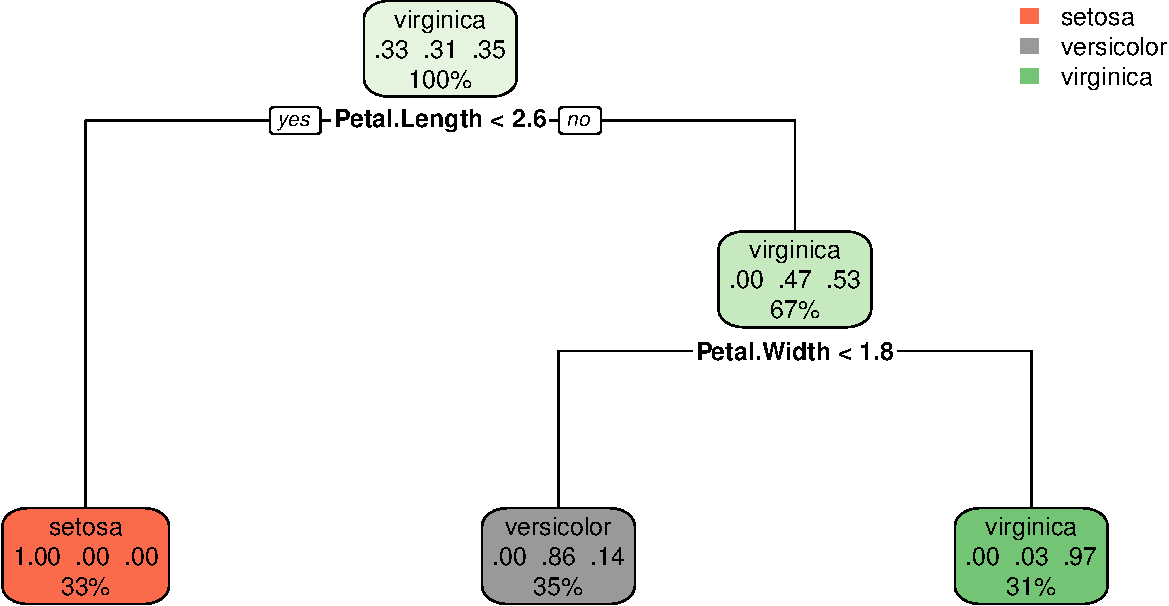
\includegraphics{EksploracjaDanych_files/figure-latex/unnamed-chunk-18-1.pdf}
\caption{\label{fig:unnamed-chunk-18}Drzewo klasyfikacyjne po przycięciu}
\end{figure}

\textbf{Ocena dopasowania modelu}

Na koniec budowy modelu należy sprawdzić jego jakość na zbiorze testowym.

\begin{Shaded}
\begin{Highlighting}[]
\NormalTok{pred.class2 <-}\StringTok{ }\KeywordTok{predict}\NormalTok{(mod.rpart2,}
                       \DataTypeTok{newdata =}\NormalTok{ dt.test,}
                       \DataTypeTok{type =} \StringTok{"class"}\NormalTok{)}
\NormalTok{tab2 <-}\StringTok{ }\KeywordTok{table}\NormalTok{(}\DataTypeTok{predykcja =}\NormalTok{ pred.class2, }\DataTypeTok{obserwacja =}\NormalTok{ dt.test}\OperatorTok{$}\NormalTok{Species)}
\NormalTok{tab2}
\end{Highlighting}
\end{Shaded}

\begin{verbatim}
##             obserwacja
## predykcja    setosa versicolor virginica
##   setosa         13          0         0
##   versicolor      0         16         0
##   virginica       0          1        15
\end{verbatim}

Mimo przycięcia drzewa, klasyfikacja pozostaje na niezmienionym poziomie. Odsetek poprawnych klasyfikacji możemy oszacować za pomocą

\begin{Shaded}
\begin{Highlighting}[]
\KeywordTok{round}\NormalTok{(}\KeywordTok{sum}\NormalTok{(}\KeywordTok{diag}\NormalTok{(tab2))}\OperatorTok{/}\KeywordTok{sum}\NormalTok{(tab2)}\OperatorTok{*}\DecValTok{100}\NormalTok{,}\DecValTok{1}\NormalTok{)}
\end{Highlighting}
\end{Shaded}

\begin{verbatim}
## [1] 97.8
\end{verbatim}

\hypertarget{inne-algorytmy-budowy-drzew-decyzyjnych-implementowane-w-r}{%
\section{\texorpdfstring{Inne algorytmy budowy drzew decyzyjnych implementowane w \textbf{R}}{Inne algorytmy budowy drzew decyzyjnych implementowane w R}}\label{inne-algorytmy-budowy-drzew-decyzyjnych-implementowane-w-r}}

Oprócz najbardziej znanego algorytmu CART implementowanego w postaci funkcji pakietu \textbf{rpart}, istnieją również inne algorytmy, które znalazły swoje implementacje w R. Są to:

\begin{itemize}
\tightlist
\item
  \emph{CHAID}\footnote{Chi-square automatic interaction detection} - algorytm przeznaczony do budowy drzew klasyfikacyjnych, gdzie zarówno zmienna wynikowa, jak i zmienne niezależne muszą być ze skali jakościowej. Główną różnicą w stosunku do drzew typu CART jest sposób budowy podziałów, oparty na teście niezależności \(\chi^2\) Pearsona. Wyboru reguły podziału dokonuje się poprzez testowanie niezależności zmiennej niezależnej z predyktorami. Reguła o największej wartości statystyki \(\chi^2\) jest stosowana w pierwszej kolejności. Implementacja tego algorytmu znajduje się w pakiecie \textbf{CHAID}\footnote{brak w oficjalnej dystrybucji CRAN} (funkcja do tworzenia drzewa o tej samej nazwie \texttt{chaid}) (Team \protect\hyperlink{ref-R-CHAID}{2015}).
\item
  \emph{Ctree}\footnote{Conditional Inference Trees} - algorytm zbliżony zasadą działania do CHAID, ponieważ również wykorzystuje testowanie do wyboru reguły podziału. Różni się jednak tym, że może być stosowany do zmiennych dowolnego typu oraz tym, że może być zarówno drzewem klasyfikacyjnym jak i regresyjnym. Implementację R-ową można znaleźć w pakietach \textbf{party} (Hothorn, Hornik, and Zeileis \protect\hyperlink{ref-R-party}{2006}) lub \textbf{partykit} (Hothorn and Zeileis \protect\hyperlink{ref-R-partykit}{2015}) - funkcją do tworzenia modelu jest \texttt{ctree}.
\item
  \emph{C4.5} - algorytm stworzony przez Quinlan (\protect\hyperlink{ref-quinlan1993}{1993}) w oparciu, o również jego autorstwa, algorytm ID3. Służy jedynie do zadań klasyfikacyjnych. W dużym uproszczeniu, dobór reguł podziału odbywa się na podstawie przyrostu informacji (patrz \protect\hyperlink{reguy-podziau}{Reguły podziału}). W przeciwieństwie do pierwotnego algorytmu ID3, C4.5 nie raczej nie przeucza drzew. Implementacja R-owa znajduje się w pakiecie \textbf{RWeka} (Hornik, Buchta, and Zeileis \protect\hyperlink{ref-R-Rweka}{2009}) - funkcja do budowy drzewa to \texttt{J48}.
\item
  \emph{C5.0} - kolejny algorytm autorstwa Kuhn and Quinlan (\protect\hyperlink{ref-R-C50}{2018}) jest usprawnieniem algorytmu C4.5, generującym mniejsze drzewa automatycznie przycinane na podstawie złożoności drzewa. Służy jedynie do zadań klasyfikacyjnych. Jest szybszy od poprzednika i pozwala na zastosowanie metody \emph{boosting}\footnote{budowa klasyfikatora w oparciu o proces iteracyjny, w którym kolejne w kolejnych iteracjach budowane są proste drzewa i przypisywane są im wagi - im gorszy klasyfikator, tym większa waga - po to aby nauczyć drzewo klasyfikować ``trudne'' przypadki}. Implementacja R-owa znajduje się w pakiecie \emph{C50}, a funkcja do budowy drzewa to \texttt{C5.0}.
\end{itemize}

\BeginKnitrBlock{example}
\protect\hypertarget{exm:przyk42}{}{\label{exm:przyk42} }W celu porównania wyników klasyfikacji na podstawie drzew decyzyjnych o różnych algorytmach, zostaną nauczone modele w oparciu o funkcje \texttt{ctree}, \texttt{J48} i \texttt{C5.0} dla tego samego zestawu danych co w przykładzie wcześniejszym \ref{exm:przyk41}.
\EndKnitrBlock{example}

\begin{itemize}
\tightlist
\item
  \textbf{Drzewo \texttt{ctree}}
\end{itemize}

Na początek ustalamy parametry ograniczające rozrost drzewa podobne jak w poprzednim przykładzie.

\begin{Shaded}
\begin{Highlighting}[]
\KeywordTok{library}\NormalTok{(partykit)}
\NormalTok{tree2 <-}\StringTok{ }\KeywordTok{ctree}\NormalTok{(Species}\OperatorTok{~}\NormalTok{., }\DataTypeTok{data =}\NormalTok{ dt.train,}
               \DataTypeTok{control =} \KeywordTok{ctree_control}\NormalTok{(}\DataTypeTok{minsplit =} \DecValTok{10}\NormalTok{,}
                                       \DataTypeTok{minbucket =} \DecValTok{5}\NormalTok{,}
                                       \DataTypeTok{maxdepth =} \DecValTok{4}\NormalTok{))}
\NormalTok{tree2}
\end{Highlighting}
\end{Shaded}

\begin{verbatim}
## 
## Model formula:
## Species ~ Sepal.Length + Sepal.Width + Petal.Length + Petal.Width
## 
## Fitted party:
## [1] root
## |   [2] Petal.Length <= 1.9: setosa (n = 37, err = 0.0%)
## |   [3] Petal.Length > 1.9
## |   |   [4] Petal.Width <= 1.7
## |   |   |   [5] Petal.Length <= 4.9: versicolor (n = 32, err = 3.1%)
## |   |   |   [6] Petal.Length > 4.9: virginica (n = 6, err = 33.3%)
## |   |   [7] Petal.Width > 1.7: virginica (n = 30, err = 0.0%)
## 
## Number of inner nodes:    3
## Number of terminal nodes: 4
\end{verbatim}

\begin{Shaded}
\begin{Highlighting}[]
\KeywordTok{plot}\NormalTok{(tree2)}
\end{Highlighting}
\end{Shaded}

\begin{figure}
\centering
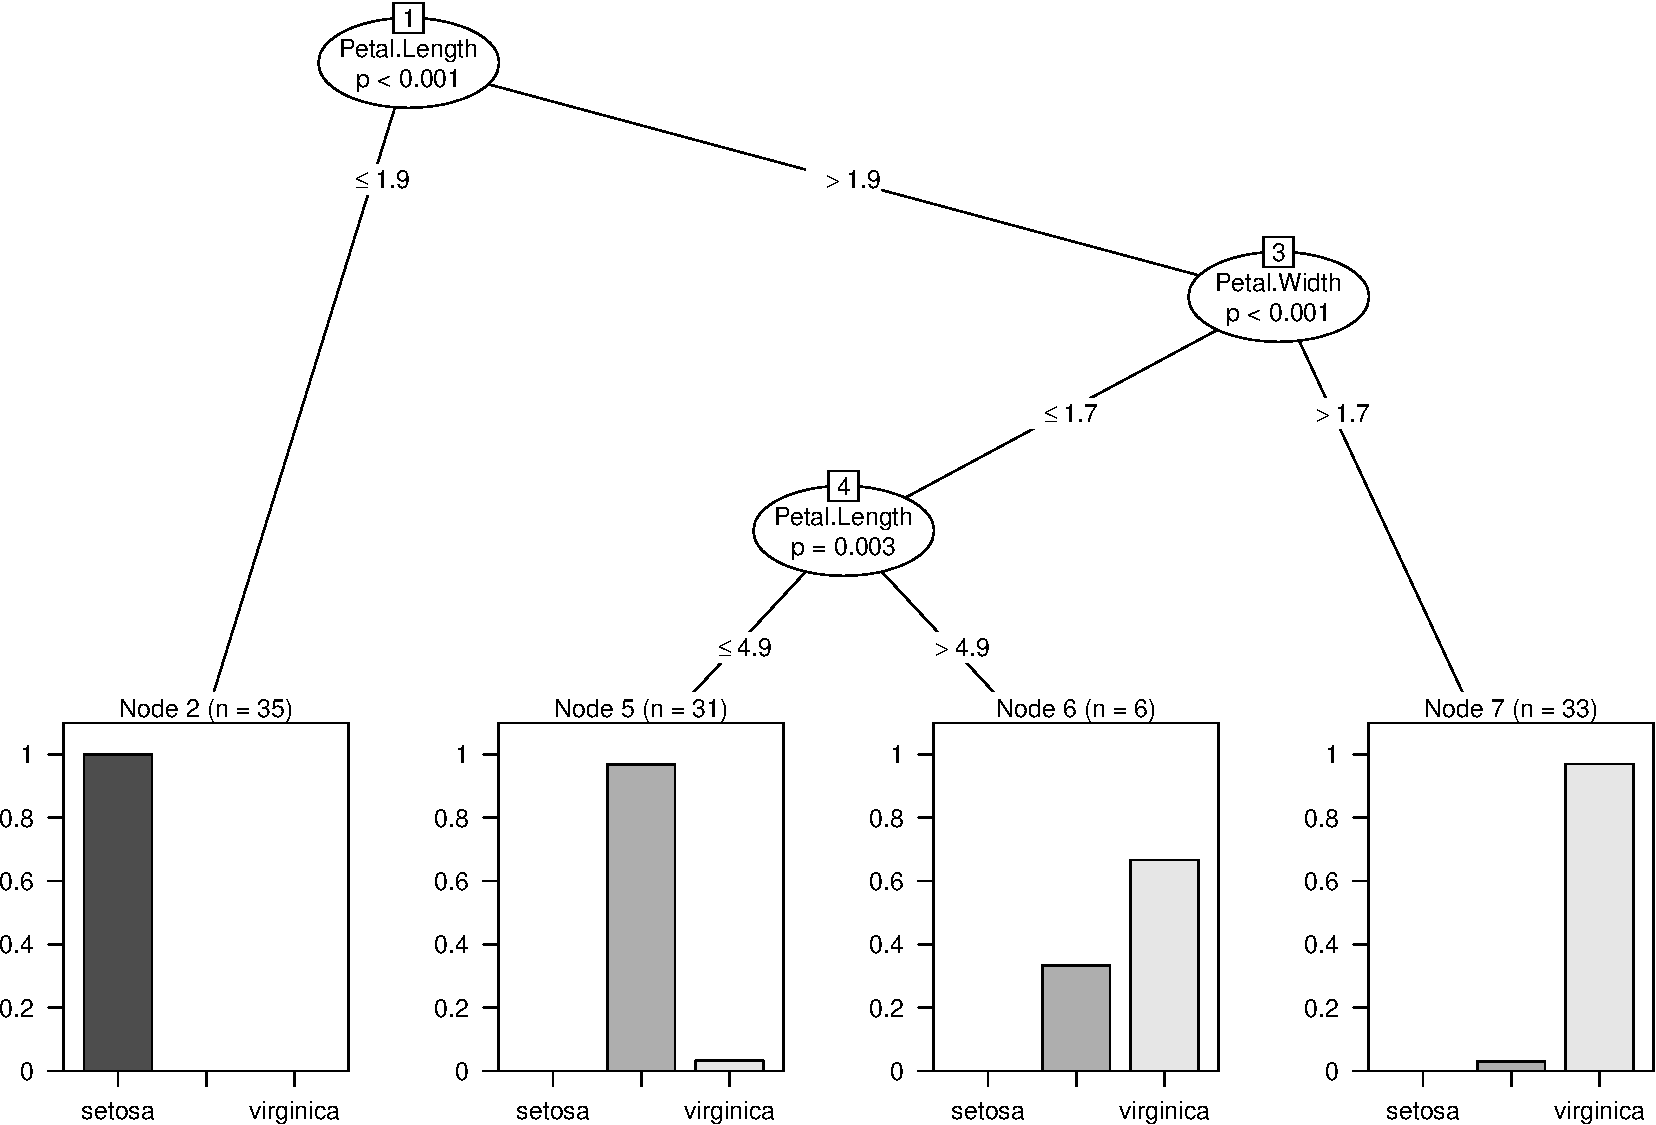
\includegraphics{EksploracjaDanych_files/figure-latex/ctree-1.pdf}
\caption{\label{fig:ctree}Wykres drzewa decyzyjnego zbudowanego metodą ctree}
\end{figure}

Wydaje się, że drzewo nie jest optymalne, ponieważ w węźle 6 obserwacje z grup \texttt{versicolor} i \texttt{virginica} są nieco pomieszane. Ostateczne oceny dokonujemy na podstawie próby testowej.

\begin{Shaded}
\begin{Highlighting}[]
\NormalTok{pred2 <-}\StringTok{ }\KeywordTok{predict}\NormalTok{(tree2, }\DataTypeTok{newdata =}\NormalTok{ dt.test)}
\NormalTok{tab <-}\StringTok{ }\KeywordTok{table}\NormalTok{(}\DataTypeTok{predykcja =}\NormalTok{ pred2, }\DataTypeTok{obserwacja =}\NormalTok{ dt.test}\OperatorTok{$}\NormalTok{Species)}
\NormalTok{tab}
\end{Highlighting}
\end{Shaded}

\begin{verbatim}
##             obserwacja
## predykcja    setosa versicolor virginica
##   setosa         13          0         0
##   versicolor      0         16         0
##   virginica       0          1        15
\end{verbatim}

Dopiero ocena jakości klasyfikacji na podstawie próby testowej pokazuje, że model zbudowany za pomocą \texttt{ctree} daje podobną precyzję jak \texttt{rpart} przycięty.

\begin{itemize}
\tightlist
\item
  \textbf{Drzewo \texttt{J48}}
\end{itemize}

W tym przypadku model sam poszukuje optymalnego rozwiązania przycinając się automatycznie.

\begin{Shaded}
\begin{Highlighting}[]
\KeywordTok{library}\NormalTok{(RWeka)}
\NormalTok{tree3 <-}\StringTok{ }\KeywordTok{J48}\NormalTok{(Species}\OperatorTok{~}\NormalTok{., }\DataTypeTok{data =}\NormalTok{ dt.train)}
\NormalTok{tree3}
\end{Highlighting}
\end{Shaded}

\begin{verbatim}
## J48 pruned tree
## ------------------
## 
## Petal.Width <= 0.6: setosa (37.0)
## Petal.Width > 0.6
## |   Petal.Width <= 1.7
## |   |   Petal.Length <= 4.9: versicolor (32.0/1.0)
## |   |   Petal.Length > 4.9
## |   |   |   Petal.Width <= 1.5: virginica (3.0)
## |   |   |   Petal.Width > 1.5: versicolor (3.0/1.0)
## |   Petal.Width > 1.7: virginica (30.0)
## 
## Number of Leaves  :  5
## 
## Size of the tree :   9
\end{verbatim}

\begin{Shaded}
\begin{Highlighting}[]
\KeywordTok{plot}\NormalTok{(tree3)}
\end{Highlighting}
\end{Shaded}

\begin{figure}
\centering
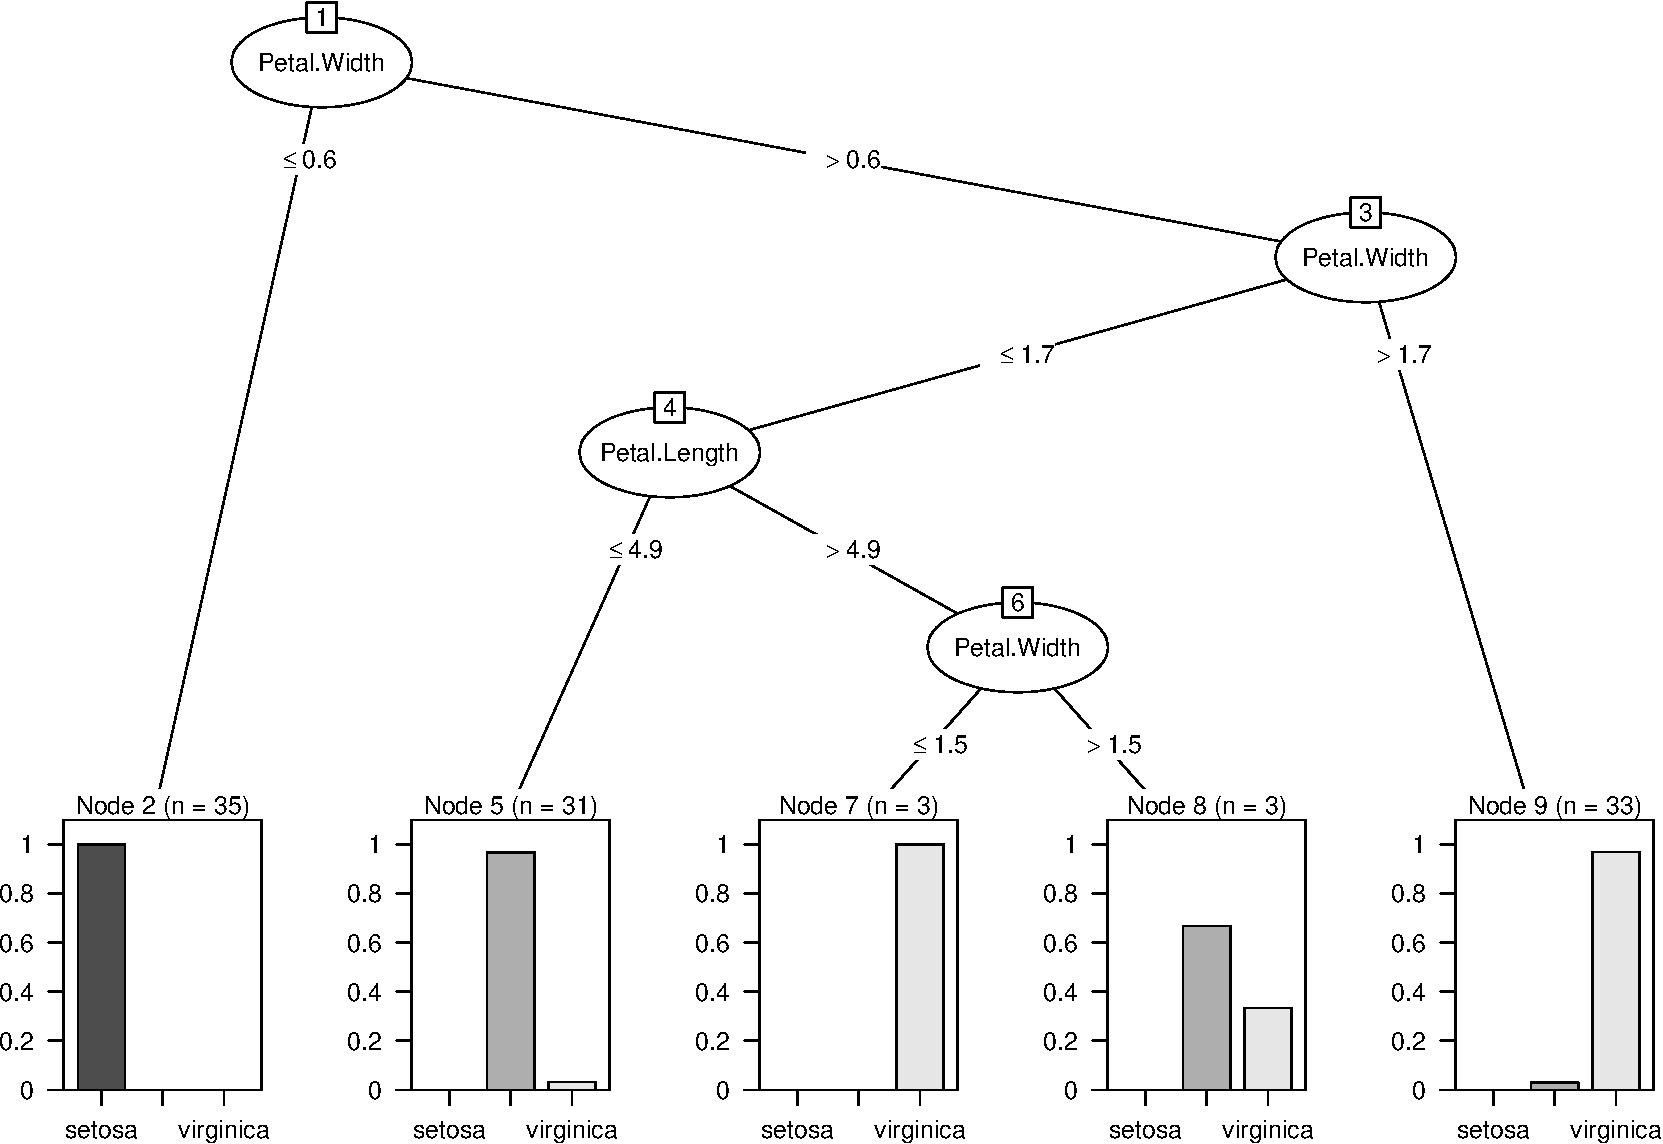
\includegraphics{EksploracjaDanych_files/figure-latex/J48-1.pdf}
\caption{\label{fig:J48}Wykres drzewa decyzyjnego zbudowanego metodą J48}
\end{figure}

Drzewo jest nieco bardziej rozbudowane niż \texttt{tree2} i \texttt{mod.rpart2}.

\begin{Shaded}
\begin{Highlighting}[]
\KeywordTok{summary}\NormalTok{(tree3)}
\end{Highlighting}
\end{Shaded}

\begin{verbatim}
## 
## === Summary ===
## 
## Correctly Classified Instances         103               98.0952 %
## Incorrectly Classified Instances         2                1.9048 %
## Kappa statistic                          0.9714
## Mean absolute error                      0.0208
## Root mean squared error                  0.1019
## Relative absolute error                  4.6776 %
## Root relative squared error             21.628  %
## Total Number of Instances              105     
## 
## === Confusion Matrix ===
## 
##   a  b  c   <-- classified as
##  37  0  0 |  a = setosa
##   0 33  0 |  b = versicolor
##   0  2 33 |  c = virginica
\end{verbatim}

Podsumowanie dopasowania drzewa na próbie uczącej jest bardzo dobre, bo poprawnych klasyfikacji jest ponad 98\%. Oceny dopasowania i tak dokonujemy na zbiorze testowym.

\begin{Shaded}
\begin{Highlighting}[]
\NormalTok{pred3 <-}\StringTok{ }\KeywordTok{predict}\NormalTok{(tree3, }\DataTypeTok{newdata =}\NormalTok{ dt.test)}
\NormalTok{tab <-}\StringTok{ }\KeywordTok{table}\NormalTok{(}\DataTypeTok{predykcja =}\NormalTok{ pred3, }\DataTypeTok{obserwacja =}\NormalTok{ dt.test}\OperatorTok{$}\NormalTok{Species)}
\NormalTok{tab}
\end{Highlighting}
\end{Shaded}

\begin{verbatim}
##             obserwacja
## predykcja    setosa versicolor virginica
##   setosa         13          0         0
##   versicolor      0         16         0
##   virginica       0          1        15
\end{verbatim}

Otrzymujemy identyczną macierz klasyfikacji jak w poprzednich przypadkach.

\begin{itemize}
\tightlist
\item
  \textbf{Drzewo \texttt{C50}}
\end{itemize}

Tym razem również nie trzeba ustawiać parametrów drzewa, ponieważ algorytm działa tak aby zapobiec rozrostowi drzewa przy jednoczesnej wysokiej poprawności klasyfikacji.

\begin{Shaded}
\begin{Highlighting}[]
\KeywordTok{library}\NormalTok{(C50)}
\NormalTok{tree4 <-}\StringTok{ }\KeywordTok{C5.0}\NormalTok{(Species}\OperatorTok{~}\NormalTok{., }\DataTypeTok{data =}\NormalTok{ dt.train)}
\KeywordTok{summary}\NormalTok{(tree4)}
\end{Highlighting}
\end{Shaded}

\begin{verbatim}
## 
## Call:
## C5.0.formula(formula = Species ~ ., data = dt.train)
## 
## 
## C5.0 [Release 2.07 GPL Edition]      Tue Apr 16 12:14:35 2019
## -------------------------------
## 
## Class specified by attribute `outcome'
## 
## Read 105 cases (5 attributes) from undefined.data
## 
## Decision tree:
## 
## Petal.Length <= 1.9: setosa (37)
## Petal.Length > 1.9:
## :...Petal.Width > 1.7: virginica (30)
##     Petal.Width <= 1.7:
##     :...Petal.Length <= 4.9: versicolor (32/1)
##         Petal.Length > 4.9: virginica (6/2)
## 
## 
## Evaluation on training data (105 cases):
## 
##      Decision Tree   
##    ----------------  
##    Size      Errors  
## 
##       4    3( 2.9%)   <<
## 
## 
##     (a)   (b)   (c)    <-classified as
##    ----  ----  ----
##      37                (a): class setosa
##            31     2    (b): class versicolor
##             1    34    (c): class virginica
## 
## 
##  Attribute usage:
## 
##  100.00% Petal.Length
##   64.76% Petal.Width
## 
## 
## Time: 0.0 secs
\end{verbatim}

Otrzymujemy identyczne drzewo jak w przypadku zastosowania algorytmu \texttt{ctree}.

\begin{Shaded}
\begin{Highlighting}[]
\KeywordTok{plot}\NormalTok{(tree4)}
\end{Highlighting}
\end{Shaded}

\begin{figure}
\centering
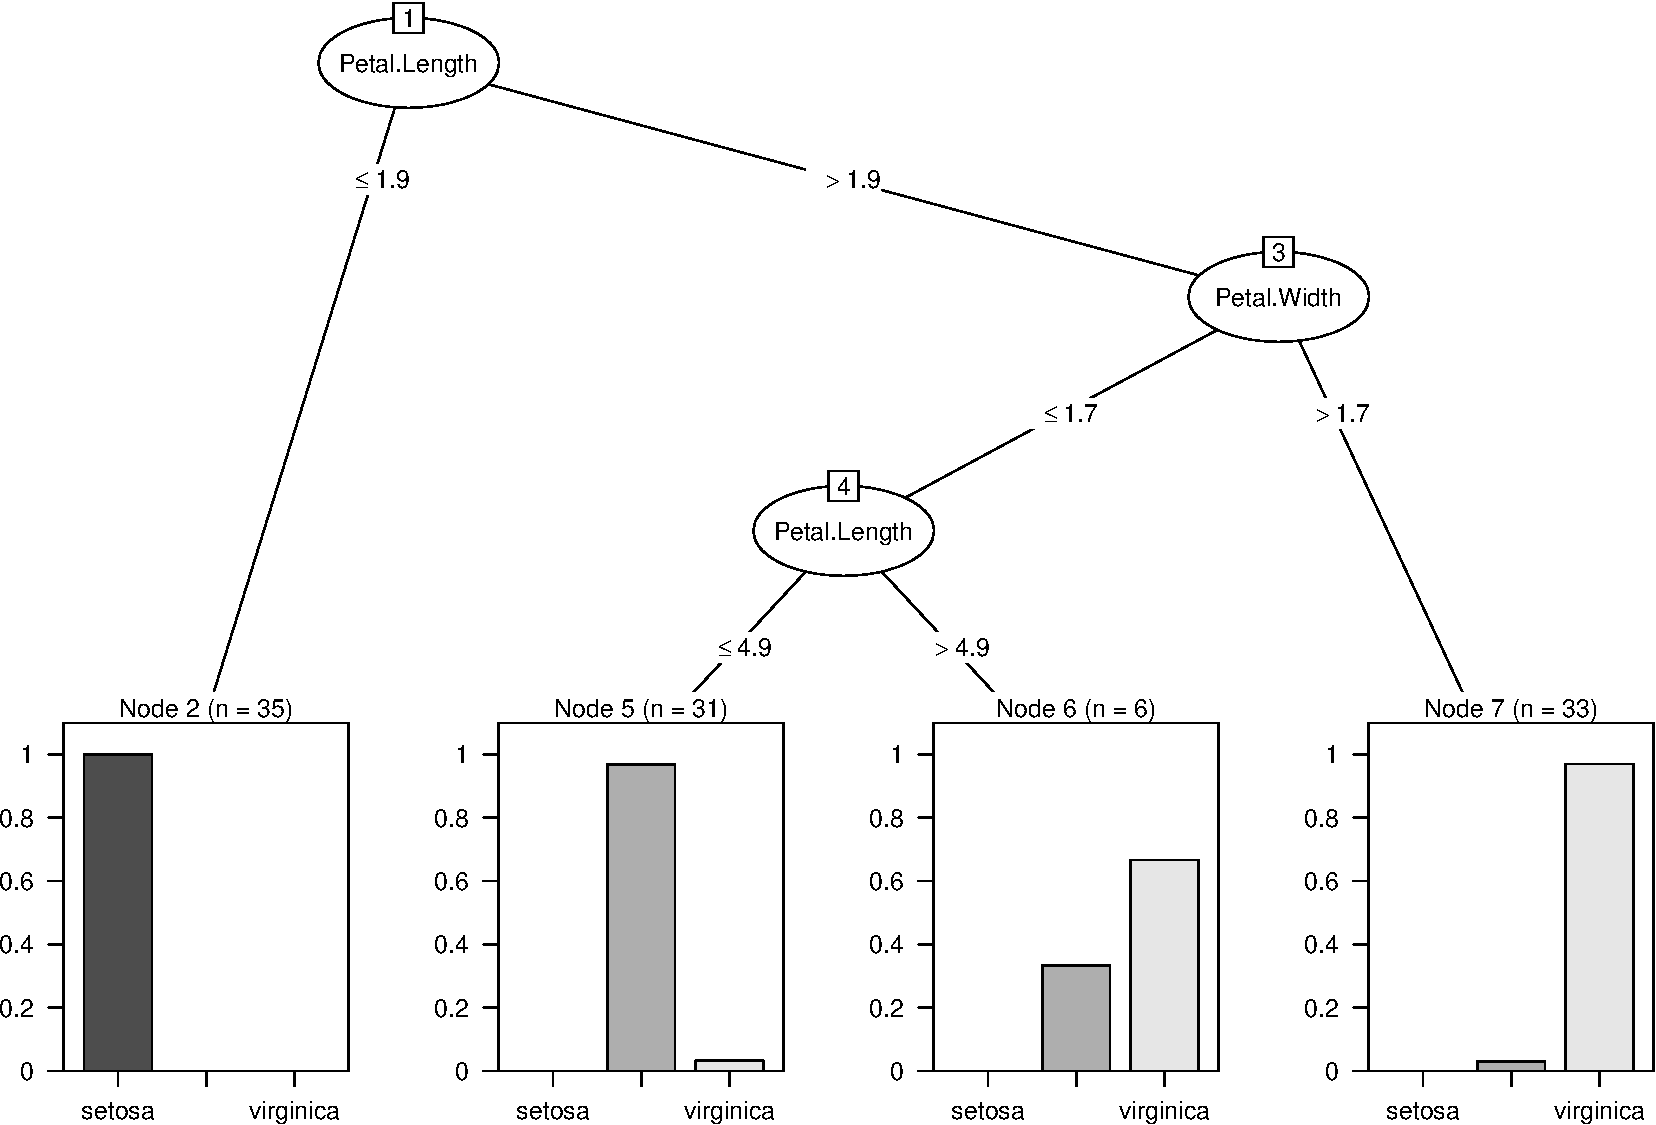
\includegraphics{EksploracjaDanych_files/figure-latex/C50-1.pdf}
\caption{\label{fig:C50}Wykres drzewa decyzyjnego zbudowanego metodą C5.0}
\end{figure}

Dla pewności przeprowadzimy sprawdzenie na zbiorze testowym.

\begin{Shaded}
\begin{Highlighting}[]
\NormalTok{pred4 <-}\StringTok{ }\KeywordTok{predict}\NormalTok{(tree4, }\DataTypeTok{newdata =}\NormalTok{ dt.test)}
\NormalTok{tab <-}\StringTok{ }\KeywordTok{table}\NormalTok{(}\DataTypeTok{predykcja =}\NormalTok{ pred4, }\DataTypeTok{obserwacja =}\NormalTok{ dt.test}\OperatorTok{$}\NormalTok{Species)}
\NormalTok{tab}
\end{Highlighting}
\end{Shaded}

\begin{verbatim}
##             obserwacja
## predykcja    setosa versicolor virginica
##   setosa         13          0         0
##   versicolor      0         16         0
##   virginica       0          1        15
\end{verbatim}

\hypertarget{pochodne-drzew-decyzyjnych}{%
\chapter{Pochodne drzew decyzyjnych}\label{pochodne-drzew-decyzyjnych}}

Przykład zastosowania drzew decyzyjnych na zbiorze \texttt{iris} w poprzednich \protect\hyperlink{przyk41}{przykładach} może skłaniać do przypuszczenia, że drzewa decyzyjne zawsze dobrze radzą sobie z predykcją wartości wynikowej. Niestety w przykładach nieco bardziej skomplikowanych, gdzie chociażby klasy zmiennej wynikowej nie są tak wyraźnie separowalne, drzewa decyzyjne wypadają gorzej w porównaniu z innymi modelami nadzorowanego uczenia maszynowego.

I tak u podstaw metod bazujących na prostych drzewach decyzyjnych stał pomysł, że skoro jedno drzewo nie ma wystarczających własności predykcyjnych, to może zastosowanie wielu drzew połączonych w pewien sposób poprawi je. Tak powstały metody \emph{bagging}, \emph{random forest} i \emph{boosting}\footnote{chyba tylko dla drugiej metody istniej dobre polskie tłumaczenie nazwy - las losowy}. Należy zaznaczyć, że metody znajdują swoje zastosowanie również w innych modelach nadzorowanego uczenia maszynowego.

\hypertarget{bagging}{%
\section{Bagging}\label{bagging}}

Technika ta została wprowadzona przez Breiman (\protect\hyperlink{ref-breiman1996}{1996}) i ma na celu zmniejszenie wariancji modelu pojedynczego drzewa. Podobnie jak technika \emph{bootstrap}, w której statystyki są wyliczane na wielu próbach pobranych z tego samego rozkładu (próby), w metodzie bagging losuje się wiele prób ze zbioru uczącego (najczęściej poprzez wielokrotne losowanie próby o rozmiarze zbioru uczącego ze zwracaniem), a następnie dla każdej próby bootstrapowej buduje się drzewo. W ten sposób otrzymujemy \(B\) drzew decyzyjnych \(\hat{f}^1(x), \hat{f}^2(x),\ldots, \hat{f}^B(x)\). Na koniec poprzez uśrednienie otrzymujemy model charakteryzujący się większą precyzją
\begin{equation}
    \hat{f}_{bag}(x)=\frac1B\sum_{b=1}^B\hat{f}^b(x).
\end{equation}

Ponieważ podczas budowy drzew na podstawie prób bootstrapowych nie kontrolujemy złożoności, to w rezultacie każde z drzew może charakteryzować się dużą wariancją. Poprzez uśrednianie wyników pojedynczych drzew otrzymujemy mniejsze obciążenie ale również przy dostatecznie dużej liczbie prób (\(B\) często liczy się w setkach, czy tysiącach) zmniejszamy wariancję ``średniej'' predykcji z drzew. Oczywiście metodę tą trzeba dostosować do zadań klasyfikacyjnych, ponieważ nie istnieje średnia klasyfikacji z wielu drzew. W miejsce średniej stosuje się modę, czyli wartość dominującą.

Przyjrzyjmy się jak maszyna losuje obserwacje ze zwracaniem

\begin{Shaded}
\begin{Highlighting}[]
\NormalTok{n <-}\StringTok{ }\OtherTok{NULL}
\NormalTok{m <-}\StringTok{ }\OtherTok{NULL}
\ControlFlowTok{for}\NormalTok{(i }\ControlFlowTok{in} \DecValTok{1}\OperatorTok{:}\DecValTok{1000}\NormalTok{)\{}
\NormalTok{    x <-}\StringTok{ }\KeywordTok{sample}\NormalTok{(}\DecValTok{1}\OperatorTok{:}\DecValTok{500}\NormalTok{, }\DataTypeTok{size =} \DecValTok{500}\NormalTok{, }\DataTypeTok{replace =}\NormalTok{ T)}
\NormalTok{    y <-}\StringTok{ }\KeywordTok{setdiff}\NormalTok{(}\DecValTok{1}\OperatorTok{:}\DecValTok{500}\NormalTok{, x)}
\NormalTok{    z <-}\StringTok{ }\KeywordTok{unique}\NormalTok{(x)}
\NormalTok{    n[i] <-}\StringTok{ }\KeywordTok{length}\NormalTok{(z)}
\NormalTok{    m[i] <-}\StringTok{ }\KeywordTok{length}\NormalTok{(y)}
\NormalTok{\}}
\KeywordTok{mean}\NormalTok{(n)}\OperatorTok{/}\DecValTok{500}\OperatorTok{*}\DecValTok{100}
\end{Highlighting}
\end{Shaded}

\begin{verbatim}
## [1] 63.2574
\end{verbatim}

\begin{Shaded}
\begin{Highlighting}[]
\KeywordTok{mean}\NormalTok{(m)}\OperatorTok{/}\DecValTok{500}\OperatorTok{*}\DecValTok{100}
\end{Highlighting}
\end{Shaded}

\begin{verbatim}
## [1] 36.7426
\end{verbatim}

Faktycznie uczenie modelu metodą bagging odbywa się średnio na 2/3 obserwacji zbioru uczącego wylosowanych do prób bootstrapowych, a pozostała 1/3 (ang. \emph{out-of-bag}) jest wykorzystana do oceny jakości predykcji.

Niewątpliwą zaletą drzew decyzyjnych była ich łatwa interpretacja. W przypadku metody bagging jest ona znacznie utrudniona, ponieważ jej wynik składa się z agregacji wielu drzew. Można natomiast ocenić ważność predyktorów (ang. \emph{variable importance}). I tak, przez obserwację spadku \(RSS\) dla baggingu regresyjnego przy zastosowaniu danego predyktora w podziałach drzewa i uśrednieniu wyniku otrzymamy wskaźnik ważności predyktora dużo lepszy niż dla pojedynczego drzewa. W przypadku baggingu klasyfikacyjnego w miejsce \(RSS\) stosujemy indeks Gini'ego.

Implementacja R-owa metody bagging znajduje się w pakiecie \textbf{ipred}, a funkcja do budowy modelu nazywa się \texttt{bagging} (Peters and Hothorn \protect\hyperlink{ref-R-ipred}{2018}). Można również stosować funkcję \texttt{randomForest} pakietu \textbf{randomForest} (Liaw and Wiener \protect\hyperlink{ref-R-las}{2002}) - powody takiego działania wyjaśnią się w podrozdziale \protect\hyperlink{lasy-losowe}{Lasy losowe}.

\BeginKnitrBlock{example}
\protect\hypertarget{exm:przyk51}{}{\label{exm:przyk51} }Tym razem cel zadania jest regresyjny i polega na ustaleniu miary tendencji centralnej ceny mieszkań w Bostonie na podstawie zmiennych umieszczonych w zbiorze \texttt{Boston} pakietu \textbf{MASS} (Venables and Ripley \protect\hyperlink{ref-R-MASS}{2002}). Zmienną zależną będzie mediana cen mieszkań na przedmieściach Bostonu (\texttt{medv}).
\EndKnitrBlock{example}

\begin{Shaded}
\begin{Highlighting}[]
\KeywordTok{library}\NormalTok{(MASS)}
\KeywordTok{head}\NormalTok{(Boston)}
\end{Highlighting}
\end{Shaded}

\begin{verbatim}
##      crim zn indus chas   nox    rm  age    dis rad tax ptratio  black
## 1 0.00632 18  2.31    0 0.538 6.575 65.2 4.0900   1 296    15.3 396.90
## 2 0.02731  0  7.07    0 0.469 6.421 78.9 4.9671   2 242    17.8 396.90
## 3 0.02729  0  7.07    0 0.469 7.185 61.1 4.9671   2 242    17.8 392.83
## 4 0.03237  0  2.18    0 0.458 6.998 45.8 6.0622   3 222    18.7 394.63
## 5 0.06905  0  2.18    0 0.458 7.147 54.2 6.0622   3 222    18.7 396.90
## 6 0.02985  0  2.18    0 0.458 6.430 58.7 6.0622   3 222    18.7 394.12
##   lstat medv
## 1  4.98 24.0
## 2  9.14 21.6
## 3  4.03 34.7
## 4  2.94 33.4
## 5  5.33 36.2
## 6  5.21 28.7
\end{verbatim}

\begin{Shaded}
\begin{Highlighting}[]
\KeywordTok{set.seed}\NormalTok{(}\DecValTok{2019}\NormalTok{)}
\NormalTok{boston.train <-}\StringTok{ }\NormalTok{Boston }\OperatorTok\StringTok{ }
\StringTok{    }\KeywordTok{sample_frac}\NormalTok{(}\DataTypeTok{size =} \DecValTok{2}\OperatorTok{/}\DecValTok{3}\NormalTok{)}
\NormalTok{boston.test <-}\StringTok{ }\KeywordTok{setdiff}\NormalTok{(Boston, boston.train)}
\end{Highlighting}
\end{Shaded}

Aby móc porównać wyniki predykcji z metody bagging, najpierw zostanie zbudowane jedno drzewo decyzyjne w oparciu o algorytm CART.

\begin{Shaded}
\begin{Highlighting}[]
\KeywordTok{library}\NormalTok{(rpart)}
\KeywordTok{library}\NormalTok{(rpart.plot)}
\NormalTok{boston.rpart <-}\StringTok{ }\KeywordTok{rpart}\NormalTok{(medv}\OperatorTok{~}\NormalTok{., }\DataTypeTok{data =}\NormalTok{ boston.train)}
\NormalTok{x <-}\StringTok{ }\KeywordTok{summary}\NormalTok{(boston.rpart)}
\end{Highlighting}
\end{Shaded}

\begin{verbatim}
## Call:
## rpart(formula = medv ~ ., data = boston.train)
##   n= 337 
## 
##            CP nsplit rel error    xerror       xstd
## 1  0.43506104      0 1.0000000 1.0037495 0.10496568
## 2  0.21114710      1 0.5649390 0.6856438 0.07732133
## 3  0.05641774      2 0.3537919 0.4393220 0.05974589
## 4  0.04154842      3 0.2973741 0.3726563 0.05716622
## 5  0.02707678      4 0.2558257 0.3520312 0.05569786
## 6  0.01489117      5 0.2287489 0.3238915 0.05681943
## 7  0.01202564      6 0.2138578 0.2922610 0.05311293
## 8  0.01057622      7 0.2018321 0.2889364 0.05318206
## 9  0.01031677      8 0.1912559 0.2838433 0.05152251
## 10 0.01006729      9 0.1809391 0.2838187 0.05152098
## 11 0.01000000     10 0.1708718 0.2815210 0.05152993
## 
## Variable importance
##   lstat     nox   indus    crim     tax      rm     age     dis ptratio 
##      24      13      13      13      11      10      10       2       2 
##     rad   black 
##       1       1 
## 
## Node number 1: 337 observations,    complexity param=0.435061
##   mean=22.61157, MSE=79.33004 
##   left son=2 (186 obs) right son=3 (151 obs)
##   Primary splits:
##       lstat   < 10.02    to the right, improve=0.4350610, (0 missing)
##       rm      < 6.8375   to the left,  improve=0.4305766, (0 missing)
##       indus   < 6.66     to the right, improve=0.2914821, (0 missing)
##       ptratio < 19.15    to the right, improve=0.2608119, (0 missing)
##       nox     < 0.5125   to the right, improve=0.2169607, (0 missing)
##   Surrogate splits:
##       indus < 7.625    to the right, agree=0.846, adj=0.656, (0 split)
##       nox   < 0.519    to the right, agree=0.828, adj=0.616, (0 split)
##       crim  < 0.12995  to the right, agree=0.786, adj=0.523, (0 split)
##       age   < 63.9     to the right, agree=0.777, adj=0.503, (0 split)
##       tax   < 377      to the right, agree=0.769, adj=0.483, (0 split)
## 
## Node number 2: 186 observations,    complexity param=0.05641774
##   mean=17.31828, MSE=19.86042 
##   left son=4 (58 obs) right son=5 (128 obs)
##   Primary splits:
##       crim  < 5.84803  to the right, improve=0.4083024, (0 missing)
##       dis   < 2.0754   to the left,  improve=0.3684093, (0 missing)
##       lstat < 14.405   to the right, improve=0.3516672, (0 missing)
##       nox   < 0.657    to the right, improve=0.3255969, (0 missing)
##       age   < 84.9     to the right, improve=0.2247741, (0 missing)
##   Surrogate splits:
##       rad   < 16       to the right, agree=0.855, adj=0.534, (0 split)
##       tax   < 551.5    to the right, agree=0.839, adj=0.483, (0 split)
##       nox   < 0.657    to the right, agree=0.828, adj=0.448, (0 split)
##       dis   < 2.0754   to the left,  agree=0.801, adj=0.362, (0 split)
##       lstat < 19.055   to the right, agree=0.796, adj=0.345, (0 split)
## 
## Node number 3: 151 observations,    complexity param=0.2111471
##   mean=29.13179, MSE=75.5574 
##   left son=6 (120 obs) right son=7 (31 obs)
##   Primary splits:
##       rm      < 7.127    to the left,  improve=0.4947648, (0 missing)
##       lstat   < 4.495    to the right, improve=0.4054324, (0 missing)
##       nox     < 0.574    to the left,  improve=0.1389706, (0 missing)
##       ptratio < 14.75    to the right, improve=0.1349232, (0 missing)
##       age     < 89.45    to the left,  improve=0.1133301, (0 missing)
##   Surrogate splits:
##       lstat   < 3.21     to the right, agree=0.841, adj=0.226, (0 split)
##       ptratio < 14.15    to the right, agree=0.828, adj=0.161, (0 split)
##       tax     < 207      to the right, agree=0.808, adj=0.065, (0 split)
##       nox     < 0.639    to the left,  agree=0.801, adj=0.032, (0 split)
## 
## Node number 4: 58 observations
##   mean=13.08793, MSE=14.14485 
## 
## Node number 5: 128 observations,    complexity param=0.01489117
##   mean=19.23516, MSE=10.66681 
##   left son=10 (61 obs) right son=11 (67 obs)
##   Primary splits:
##       lstat   < 14.405   to the right, improve=0.2915760, (0 missing)
##       dis     < 1.99235  to the left,  improve=0.2280873, (0 missing)
##       age     < 84.15    to the right, improve=0.1950219, (0 missing)
##       ptratio < 20.95    to the right, improve=0.1349341, (0 missing)
##       rm      < 5.706    to the left,  improve=0.1194638, (0 missing)
##   Surrogate splits:
##       age   < 91.15    to the right, agree=0.758, adj=0.492, (0 split)
##       dis   < 2.0418   to the left,  agree=0.664, adj=0.295, (0 split)
##       nox   < 0.607    to the right, agree=0.633, adj=0.230, (0 split)
##       indus < 18.84    to the right, agree=0.625, adj=0.213, (0 split)
##       rm    < 5.703    to the left,  agree=0.617, adj=0.197, (0 split)
## 
## Node number 6: 120 observations,    complexity param=0.04154842
##   mean=26.02417, MSE=34.39883 
##   left son=12 (98 obs) right son=13 (22 obs)
##   Primary splits:
##       lstat < 5.145    to the right, improve=0.2690898, (0 missing)
##       dis   < 2.0891   to the right, improve=0.2163813, (0 missing)
##       rm    < 6.543    to the left,  improve=0.2036454, (0 missing)
##       age   < 89.45    to the left,  improve=0.1796977, (0 missing)
##       tax   < 548      to the left,  improve=0.1751322, (0 missing)
##   Surrogate splits:
##       zn    < 92.5     to the left,  agree=0.833, adj=0.091, (0 split)
##       nox   < 0.4035   to the right, agree=0.833, adj=0.091, (0 split)
##       indus < 1.495    to the right, agree=0.825, adj=0.045, (0 split)
##       dis   < 1.48495  to the right, agree=0.825, adj=0.045, (0 split)
## 
## Node number 7: 31 observations,    complexity param=0.02707678
##   mean=41.16129, MSE=52.78882 
##   left son=14 (11 obs) right son=15 (20 obs)
##   Primary splits:
##       rm      < 7.437    to the left,  improve=0.4423448, (0 missing)
##       lstat   < 5.185    to the right, improve=0.3125696, (0 missing)
##       ptratio < 15.05    to the right, improve=0.1896089, (0 missing)
##       black   < 392.715  to the right, improve=0.1133472, (0 missing)
##       age     < 37.6     to the right, improve=0.0737298, (0 missing)
##   Surrogate splits:
##       lstat < 4.635    to the right, agree=0.774, adj=0.364, (0 split)
##       indus < 2.32     to the left,  agree=0.742, adj=0.273, (0 split)
##       dis   < 5.9736   to the right, agree=0.710, adj=0.182, (0 split)
##       black < 390.095  to the right, agree=0.710, adj=0.182, (0 split)
##       crim  < 0.10593  to the left,  agree=0.677, adj=0.091, (0 split)
## 
## Node number 10: 61 observations
##   mean=17.38689, MSE=8.122779 
## 
## Node number 11: 67 observations
##   mean=20.91791, MSE=7.041172 
## 
## Node number 12: 98 observations,    complexity param=0.01202564
##   mean=24.58265, MSE=20.9745 
##   left son=24 (64 obs) right son=25 (34 obs)
##   Primary splits:
##       rm    < 6.543    to the left,  improve=0.1564077, (0 missing)
##       black < 364.385  to the right, improve=0.1331323, (0 missing)
##       age   < 89.45    to the left,  improve=0.1241124, (0 missing)
##       tax   < 223.5    to the right, improve=0.1204819, (0 missing)
##       dis   < 4.46815  to the right, improve=0.1048755, (0 missing)
##   Surrogate splits:
##       dis   < 3.6589   to the right, agree=0.704, adj=0.147, (0 split)
##       rad   < 6.5      to the left,  agree=0.704, adj=0.147, (0 split)
##       age   < 68.9     to the left,  agree=0.694, adj=0.118, (0 split)
##       indus < 1.605    to the right, agree=0.673, adj=0.059, (0 split)
##       nox   < 0.4045   to the right, agree=0.673, adj=0.059, (0 split)
## 
## Node number 13: 22 observations,    complexity param=0.01031677
##   mean=32.44545, MSE=43.70884 
##   left son=26 (15 obs) right son=27 (7 obs)
##   Primary splits:
##       tax   < 364      to the left,  improve=0.2868266, (0 missing)
##       lstat < 3.855    to the right, improve=0.2413545, (0 missing)
##       age   < 31.85    to the left,  improve=0.1598075, (0 missing)
##       dis   < 5.4085   to the right, improve=0.1258591, (0 missing)
##       black < 381.59   to the right, improve=0.1052855, (0 missing)
##   Surrogate splits:
##       crim  < 2.6956   to the left,  agree=0.773, adj=0.286, (0 split)
##       indus < 14       to the left,  agree=0.773, adj=0.286, (0 split)
##       nox   < 0.5875   to the left,  agree=0.773, adj=0.286, (0 split)
##       age   < 89.65    to the left,  agree=0.773, adj=0.286, (0 split)
##       dis   < 2.3371   to the right, agree=0.773, adj=0.286, (0 split)
## 
## Node number 14: 11 observations
##   mean=34.64545, MSE=3.304298 
## 
## Node number 15: 20 observations,    complexity param=0.01057622
##   mean=44.745, MSE=43.81147 
##   left son=30 (12 obs) right son=31 (8 obs)
##   Primary splits:
##       ptratio < 15.4     to the right, improve=0.3226860, (0 missing)
##       rad     < 6        to the right, improve=0.2170243, (0 missing)
##       tax     < 270      to the right, improve=0.1545997, (0 missing)
##       age     < 71.85    to the right, improve=0.1331209, (0 missing)
##       zn      < 10       to the left,  improve=0.1328727, (0 missing)
##   Surrogate splits:
##       zn   < 10       to the left,  agree=0.80, adj=0.500, (0 split)
##       nox  < 0.541    to the left,  agree=0.80, adj=0.500, (0 split)
##       age  < 86.7     to the left,  agree=0.80, adj=0.500, (0 split)
##       dis  < 2.5813   to the right, agree=0.80, adj=0.500, (0 split)
##       crim < 0.45114  to the left,  agree=0.75, adj=0.375, (0 split)
## 
## Node number 24: 64 observations,    complexity param=0.01006729
##   mean=23.2625, MSE=21.96891 
##   left son=48 (57 obs) right son=49 (7 obs)
##   Primary splits:
##       indus < 14.48    to the left,  improve=0.19142190, (0 missing)
##       crim  < 0.841845 to the left,  improve=0.17407590, (0 missing)
##       black < 374.635  to the right, improve=0.14590640, (0 missing)
##       dis   < 2.6499   to the right, improve=0.13374910, (0 missing)
##       age   < 79.85    to the left,  improve=0.08856433, (0 missing)
##   Surrogate splits:
##       crim  < 1.163695 to the left,  agree=0.984, adj=0.857, (0 split)
##       nox   < 0.589    to the left,  agree=0.984, adj=0.857, (0 split)
##       age   < 84.35    to the left,  agree=0.984, adj=0.857, (0 split)
##       dis   < 2.28545  to the right, agree=0.969, adj=0.714, (0 split)
##       black < 361.635  to the right, agree=0.969, adj=0.714, (0 split)
## 
## Node number 25: 34 observations
##   mean=27.06765, MSE=9.646894 
## 
## Node number 26: 15 observations
##   mean=30.02667, MSE=14.56062 
## 
## Node number 27: 7 observations
##   mean=37.62857, MSE=66.76776 
## 
## Node number 30: 12 observations
##   mean=41.675, MSE=48.28521 
## 
## Node number 31: 8 observations
##   mean=49.35, MSE=1.7575 
## 
## Node number 48: 57 observations
##   mean=22.54386, MSE=10.87053 
## 
## Node number 49: 7 observations
##   mean=29.11429, MSE=73.89265
\end{verbatim}

\begin{Shaded}
\begin{Highlighting}[]
\KeywordTok{rpart.plot}\NormalTok{(boston.rpart)}
\end{Highlighting}
\end{Shaded}

\begin{figure}
\centering
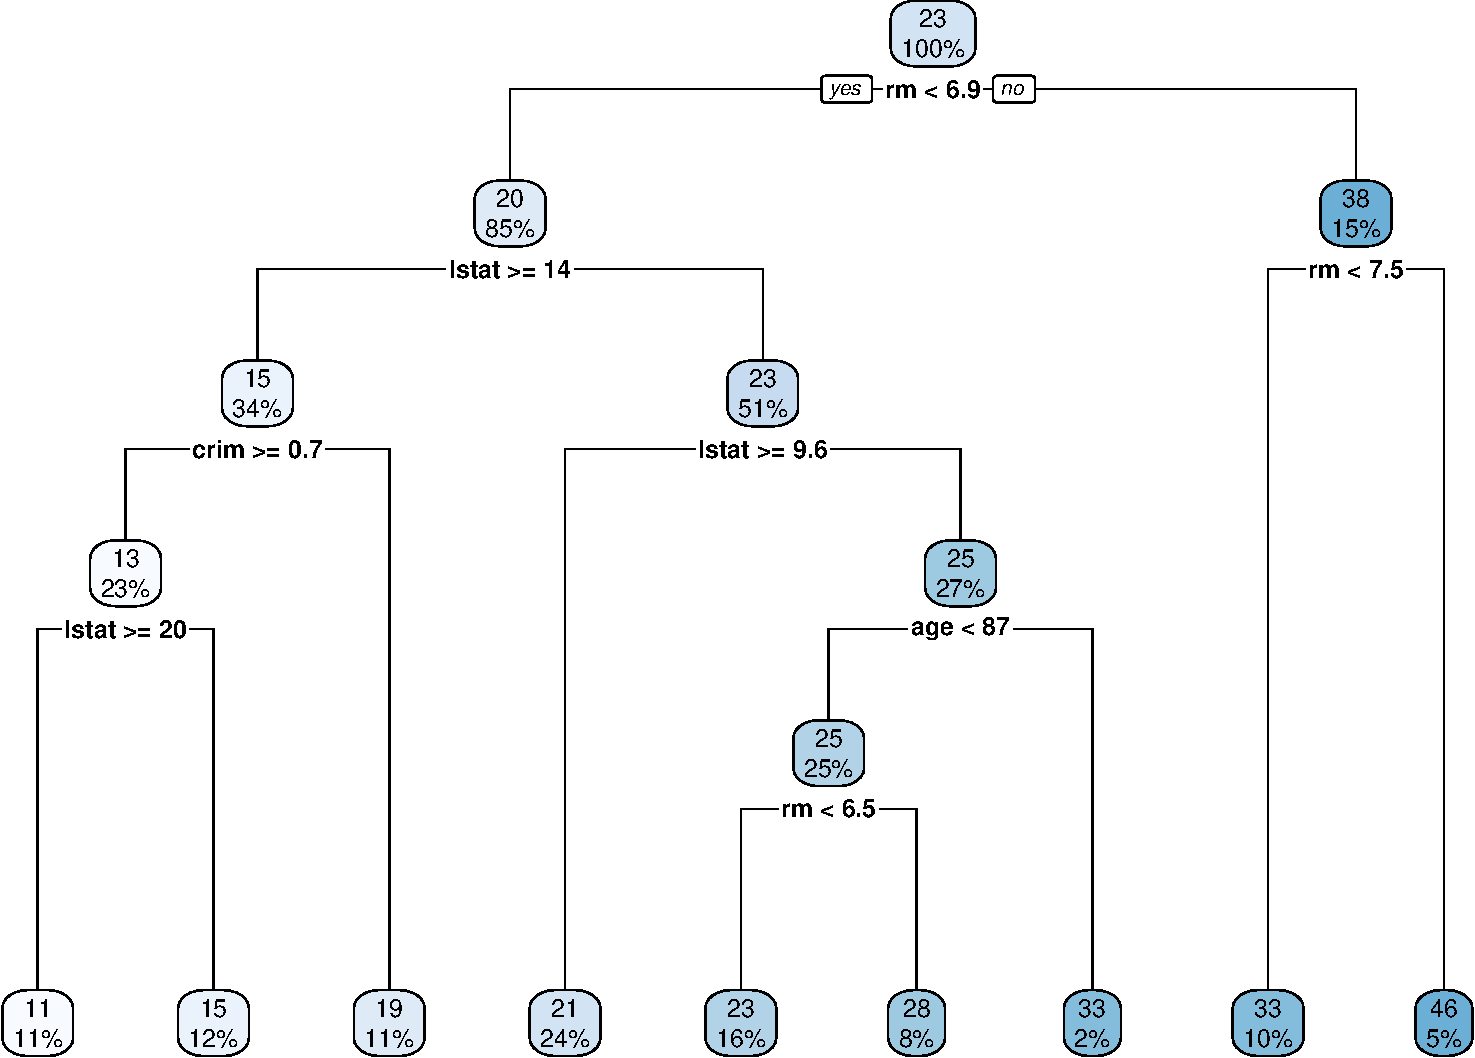
\includegraphics{EksploracjaDanych_files/figure-latex/unnamed-chunk-32-1.pdf}
\caption{\label{fig:unnamed-chunk-32}Drzewo regresyjne pełne}
\end{figure}

Przycinamy drzewo\ldots{}

\begin{Shaded}
\begin{Highlighting}[]
\KeywordTok{printcp}\NormalTok{(boston.rpart)}
\end{Highlighting}
\end{Shaded}

\begin{verbatim}
## 
## Regression tree:
## rpart(formula = medv ~ ., data = boston.train)
## 
## Variables actually used in tree construction:
## [1] crim    indus   lstat   ptratio rm      tax    
## 
## Root node error: 26734/337 = 79.33
## 
## n= 337 
## 
##          CP nsplit rel error  xerror     xstd
## 1  0.435061      0   1.00000 1.00375 0.104966
## 2  0.211147      1   0.56494 0.68564 0.077321
## 3  0.056418      2   0.35379 0.43932 0.059746
## 4  0.041548      3   0.29737 0.37266 0.057166
## 5  0.027077      4   0.25583 0.35203 0.055698
## 6  0.014891      5   0.22875 0.32389 0.056819
## 7  0.012026      6   0.21386 0.29226 0.053113
## 8  0.010576      7   0.20183 0.28894 0.053182
## 9  0.010317      8   0.19126 0.28384 0.051523
## 10 0.010067      9   0.18094 0.28382 0.051521
## 11 0.010000     10   0.17087 0.28152 0.051530
\end{verbatim}

\begin{Shaded}
\begin{Highlighting}[]
\KeywordTok{plotcp}\NormalTok{(boston.rpart)}
\end{Highlighting}
\end{Shaded}

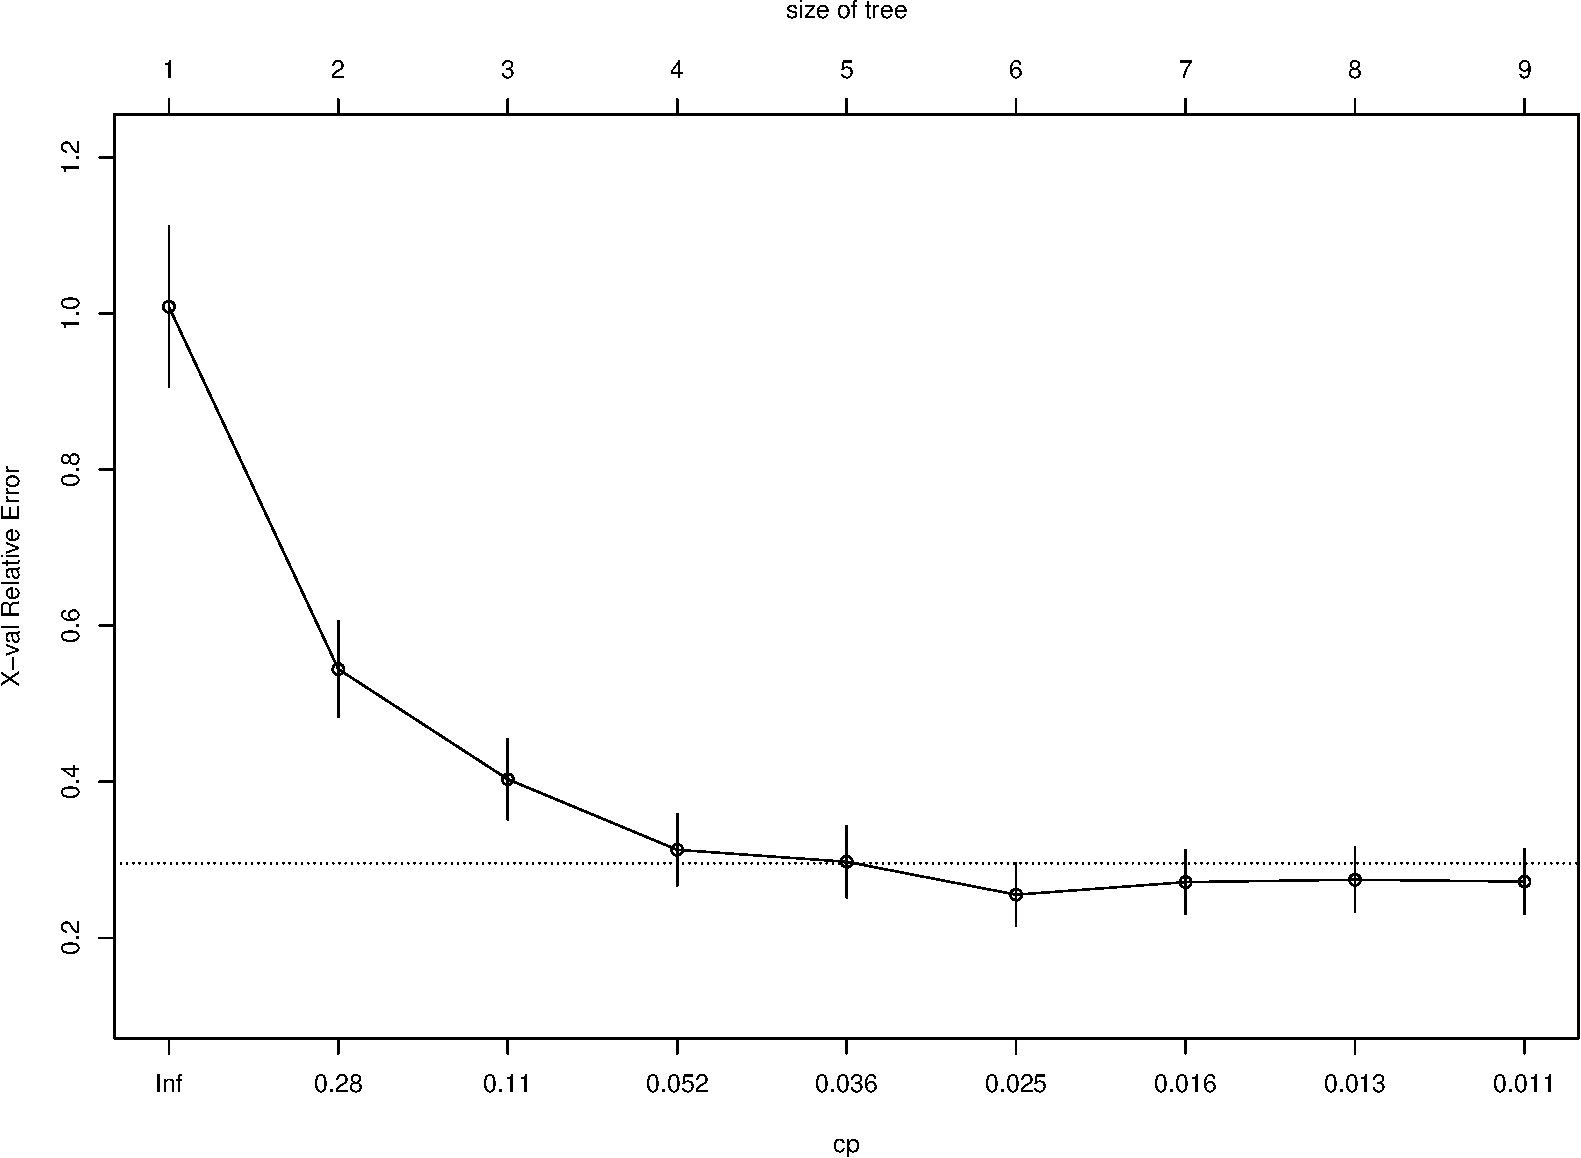
\includegraphics{EksploracjaDanych_files/figure-latex/unnamed-chunk-33-1.pdf}

\begin{Shaded}
\begin{Highlighting}[]
\NormalTok{boston.rpart2 <-}\StringTok{ }\KeywordTok{prune}\NormalTok{(boston.rpart, }\DataTypeTok{cp =} \FloatTok{0.012026}\NormalTok{)}
\end{Highlighting}
\end{Shaded}

\begin{Shaded}
\begin{Highlighting}[]
\KeywordTok{rpart.plot}\NormalTok{(boston.rpart2)}
\end{Highlighting}
\end{Shaded}

\begin{figure}
\centering
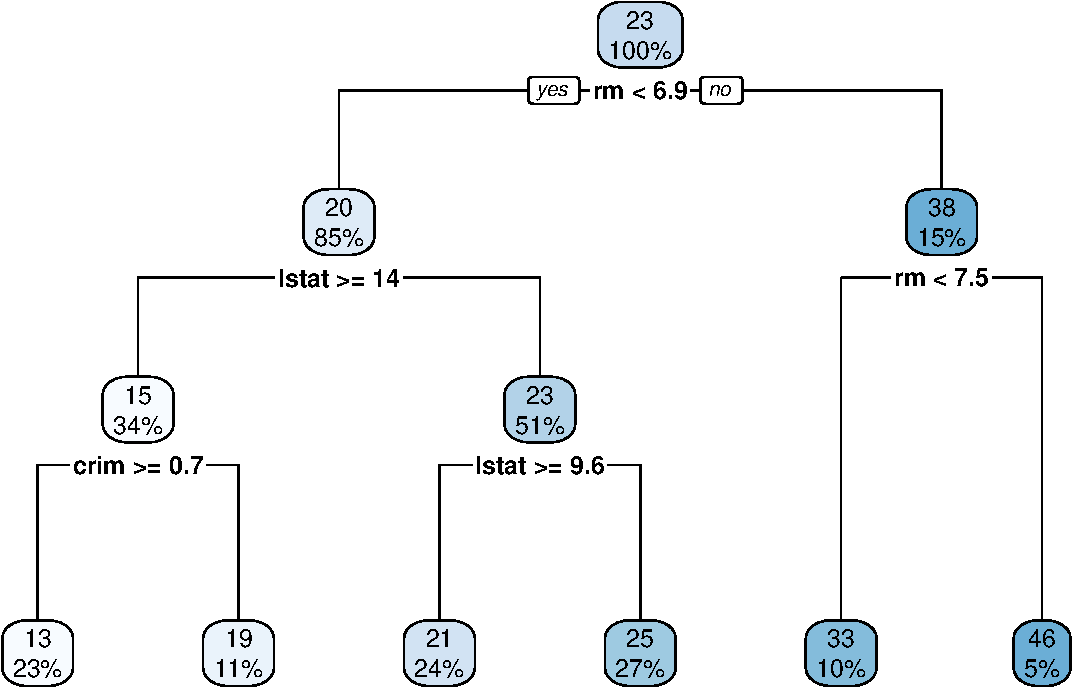
\includegraphics{EksploracjaDanych_files/figure-latex/unnamed-chunk-34-1.pdf}
\caption{\label{fig:unnamed-chunk-34}Drzewo regresyjne przycięte}
\end{figure}

Predykcja na podstawie drzewa na zbiorze testowym.

\begin{Shaded}
\begin{Highlighting}[]
\NormalTok{boston.pred <-}\StringTok{ }\KeywordTok{predict}\NormalTok{(boston.rpart2, }\DataTypeTok{newdata =}\NormalTok{ boston.test)}
\NormalTok{rmse <-}\StringTok{ }\ControlFlowTok{function}\NormalTok{(pred, obs) }\KeywordTok{sqrt}\NormalTok{(}\DecValTok{1}\OperatorTok{/}\KeywordTok{length}\NormalTok{(pred)}\OperatorTok{*}\KeywordTok{sum}\NormalTok{((pred}\OperatorTok{-}\NormalTok{obs)}\OperatorTok{^}\DecValTok{2}\NormalTok{))}
\KeywordTok{rmse}\NormalTok{(boston.pred, boston.test}\OperatorTok{$}\NormalTok{medv)}
\end{Highlighting}
\end{Shaded}

\begin{verbatim}
## [1] 4.825862
\end{verbatim}

Teraz zbudujemy model metodą bagging.

\begin{Shaded}
\begin{Highlighting}[]
\KeywordTok{library}\NormalTok{(randomForest)}
\NormalTok{boston.bag <-}\StringTok{ }\KeywordTok{randomForest}\NormalTok{(medv}\OperatorTok{~}\NormalTok{., }\DataTypeTok{data =}\NormalTok{ boston.train, }
                           \DataTypeTok{mtry =} \KeywordTok{ncol}\NormalTok{(boston.train)}\OperatorTok{-}\DecValTok{1}\NormalTok{)}
\NormalTok{boston.bag}
\end{Highlighting}
\end{Shaded}

\begin{verbatim}
## 
## Call:
##  randomForest(formula = medv ~ ., data = boston.train, mtry = ncol(boston.train) -      1) 
##                Type of random forest: regression
##                      Number of trees: 500
## No. of variables tried at each split: 13
## 
##           Mean of squared residuals: 13.06701
##                     % Var explained: 83.53
\end{verbatim}

Predykcja na podstawie modelu

\begin{Shaded}
\begin{Highlighting}[]
\NormalTok{boston.pred2 <-}\StringTok{ }\KeywordTok{predict}\NormalTok{(boston.bag, }\DataTypeTok{newdata =}\NormalTok{ boston.test)}
\KeywordTok{rmse}\NormalTok{(boston.pred2, boston.test}\OperatorTok{$}\NormalTok{medv)}
\end{Highlighting}
\end{Shaded}

\begin{verbatim}
## [1] 3.039308
\end{verbatim}

Zatem predykcja na podstawie modelu bagging jest nico lepsza niż z pojedynczego drzewa. Dodatkowo możemy ocenić ważność zmiennych użytych w budowie drzew.

\begin{Shaded}
\begin{Highlighting}[]
\KeywordTok{varImpPlot}\NormalTok{(boston.bag)}
\end{Highlighting}
\end{Shaded}

\begin{figure}
\centering
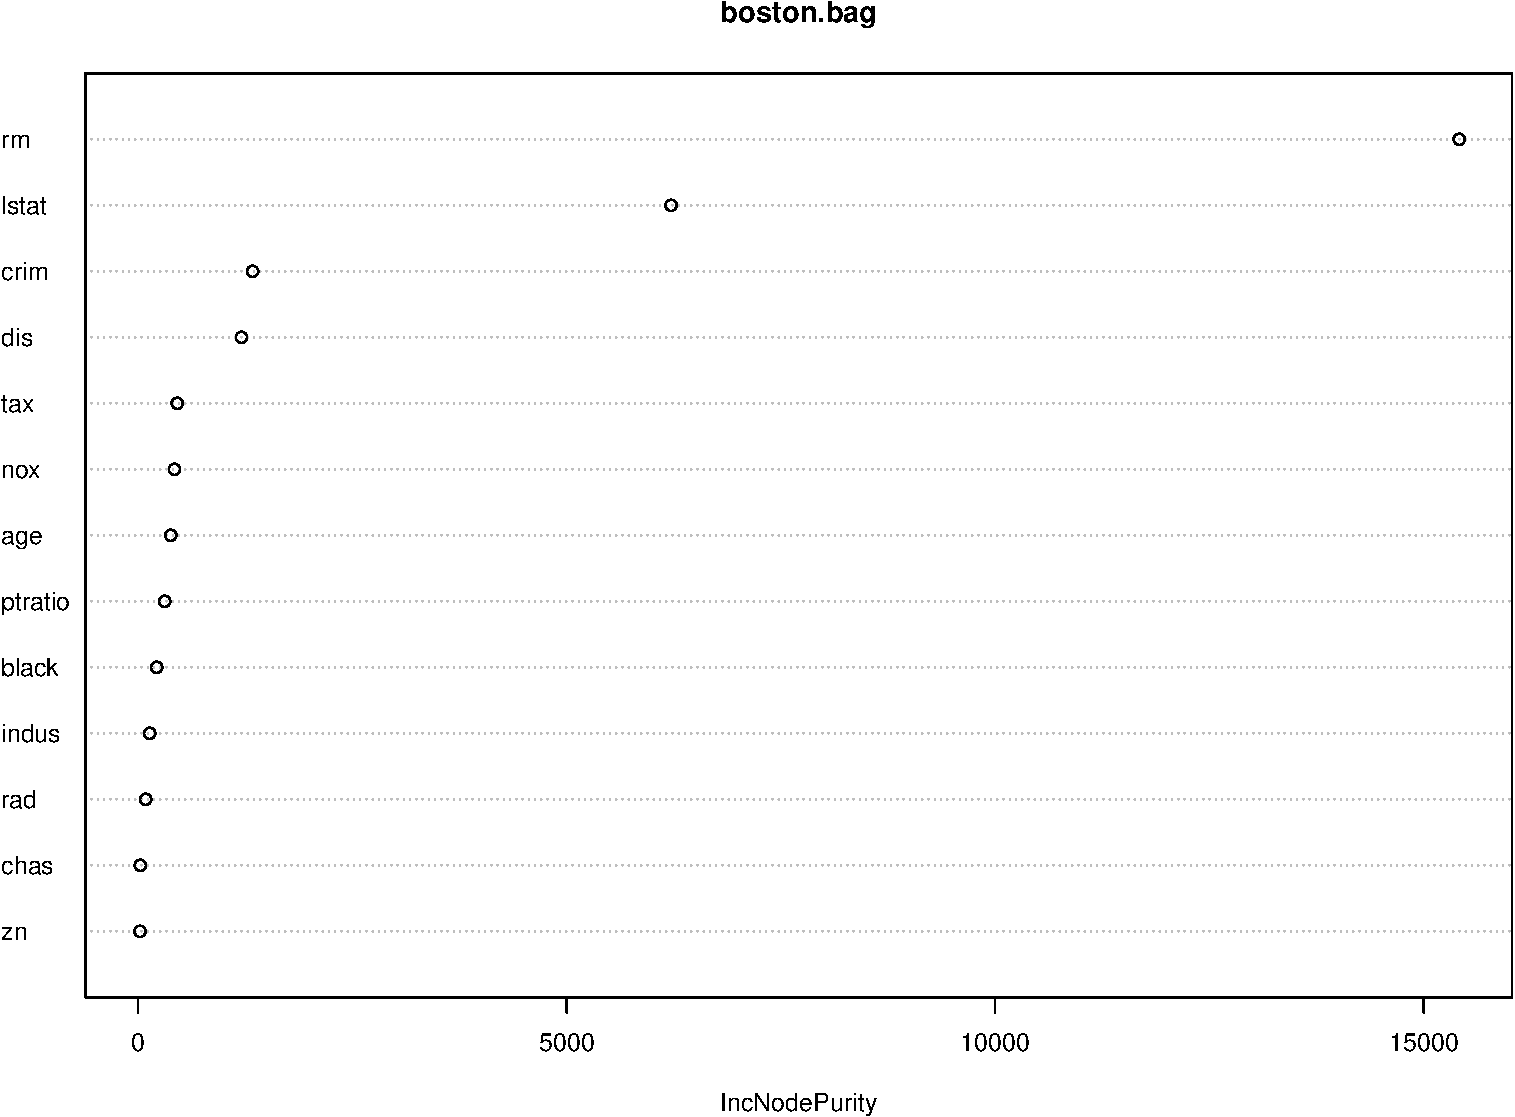
\includegraphics{EksploracjaDanych_files/figure-latex/unnamed-chunk-38-1.pdf}
\caption{\label{fig:unnamed-chunk-38}Wykres ważności predyktorów}
\end{figure}

\begin{Shaded}
\begin{Highlighting}[]
\KeywordTok{importance}\NormalTok{(boston.bag)}
\end{Highlighting}
\end{Shaded}

\begin{verbatim}
##         IncNodePurity
## crim       1200.11828
## zn           24.17836
## indus       262.33396
## chas         22.27133
## nox         417.32236
## rm         9102.58339
## age         416.48170
## dis        1494.79734
## rad         171.92103
## tax         403.66309
## ptratio     411.88528
## black       331.58495
## lstat     12137.38999
\end{verbatim}

\begin{Shaded}
\begin{Highlighting}[]
\NormalTok{x}\OperatorTok{$}\NormalTok{variable.importance}
\end{Highlighting}
\end{Shaded}

\begin{verbatim}
##      lstat        nox      indus       crim        tax         rm 
## 15197.8587  8683.8225  8325.2431  8074.7200  6991.0756  6768.5423 
##        age        dis    ptratio        rad      black         zn 
##  6538.5039  1305.3786  1193.2073   853.4309   323.8576   242.3521
\end{verbatim}

W porównaniu do ważności zmiennych dla pojedynczego drzewa widać pewne różnice.

\hypertarget{lasy-losowe}{%
\section{Lasy losowe}\label{lasy-losowe}}

Lasy losowe są uogólnieniem metody bagging, polegającą na losowaniu dla każdego drzewa wchodzącego w skład lasu \(m\) predyktorów spośród \(p\) dostępnych, a następnie budowaniu drzew z wykorzystaniem tylko tych predyktorów (Ho \protect\hyperlink{ref-ho1995}{1995}). Dzięki temu za każdy razem drzewo jest budowane w oparciu o nowy zestaw cech (najczęściej przyjmujemy \(m=\sqrt{p}\)). W przypadku modeli bagging za każdym razem najsilniejszy predyktor wchodził w skład zbioru uczącego, a co za tym idzie również uczestniczył w tworzeniu reguł podziału. Wówczas wiele drzew zawierało reguły stosujące dany atrybut, a wtedy predykcje otrzymywane za pomocą drzew były skorelowane. Dlatego nawet duża liczba prób bootstrapowych nie zapewniała poprawy precyzji. Implementacja tej metody znajduje się w pakiecie \textbf{randomForest}.

\BeginKnitrBlock{example}
\protect\hypertarget{exm:przyk52}{}{\label{exm:przyk52} }Kontynuując poprzedni przykład \ref{exm:przyk51} możemy zbudować las losowy aby przekonać się czy nastąpi poprawa predykcji zmiennej wynikowej.
\EndKnitrBlock{example}

\begin{Shaded}
\begin{Highlighting}[]
\NormalTok{boston.rf <-}\StringTok{ }\KeywordTok{randomForest}\NormalTok{(medv}\OperatorTok{~}\NormalTok{., }\DataTypeTok{data =}\NormalTok{ boston.train)}
\NormalTok{boston.rf}
\end{Highlighting}
\end{Shaded}

\begin{verbatim}
## 
## Call:
##  randomForest(formula = medv ~ ., data = boston.train) 
##                Type of random forest: regression
##                      Number of trees: 500
## No. of variables tried at each split: 4
## 
##           Mean of squared residuals: 13.09902
##                     % Var explained: 83.49
\end{verbatim}

Porównanie MSE na próbach uczących pomiędzy lasem losowym i modelem bagging wypada nieco na korzyść bagging.

\begin{Shaded}
\begin{Highlighting}[]
\NormalTok{boston.pred3 <-}\StringTok{ }\KeywordTok{predict}\NormalTok{(boston.rf, }\DataTypeTok{newdata =}\NormalTok{ boston.test)}
\KeywordTok{rmse}\NormalTok{(boston.pred3, boston.test}\OperatorTok{$}\NormalTok{medv)}
\end{Highlighting}
\end{Shaded}

\begin{verbatim}
## [1] 3.418302
\end{verbatim}

Ważność zmiennych również się nieco różni.

\begin{Shaded}
\begin{Highlighting}[]
\KeywordTok{varImpPlot}\NormalTok{(boston.rf)}
\end{Highlighting}
\end{Shaded}

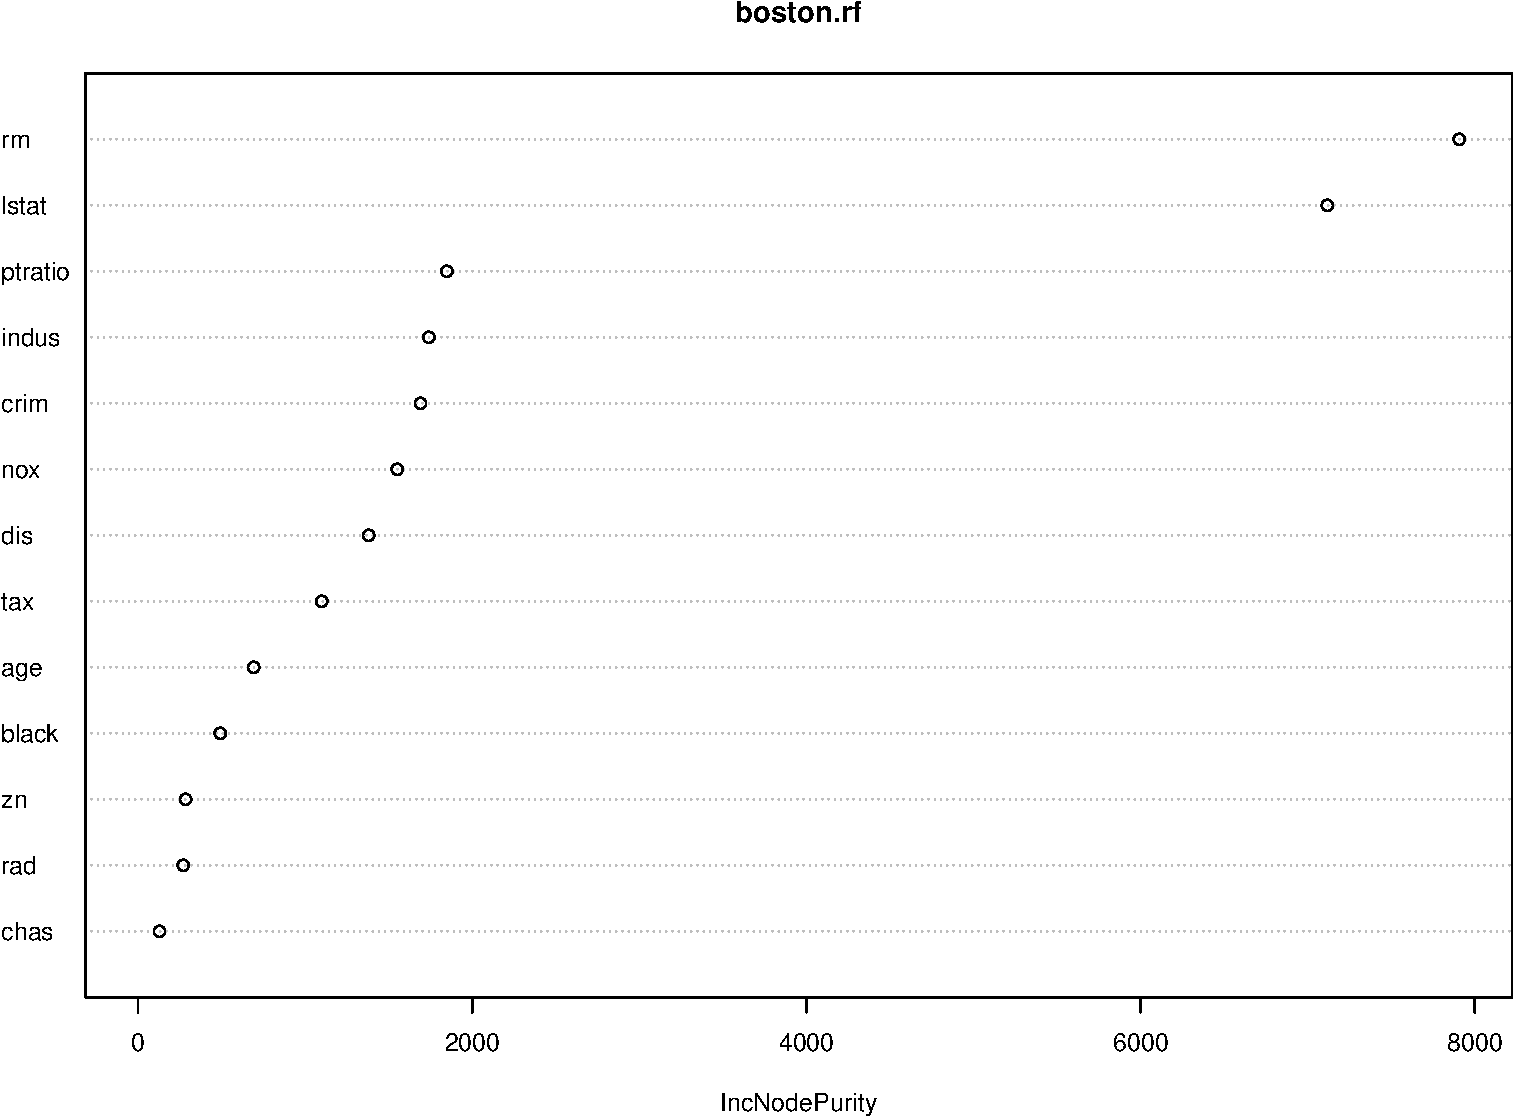
\includegraphics{EksploracjaDanych_files/figure-latex/unnamed-chunk-41-1.pdf}

\hypertarget{boosting}{%
\section{Boosting}\label{boosting}}

Rozważania na temat metody \emph{boosting} zaczęły się od pytań postawionych w publikacji Kearns and Valiant (\protect\hyperlink{ref-kearns1989}{1989}), czy da się na podstawie na podstawie zbioru słabych modeli stworzyć jeden dobry? Odpowiedzi pozytywnej na nie udzielili, najpierw Schapire (\protect\hyperlink{ref-schapire1990}{1990}), a potem Breiman (\protect\hyperlink{ref-breiman1998}{1998}). W metodzie boosting nie stosuje się prób bootstrapowych ale odpowiednio modyfikuje się drzewo wyjściowe w kolejnych krokach na tym samym zbiorze uczącym. Algorytm dla drzewa regresyjnego jest następujący:

\begin{enumerate}
\def\labelenumi{\arabic{enumi}.}
\tightlist
\item
  Ustal \(\hat{f}(x)=0\) i \(r_i=y_i\) dla każdego \(i\) w zbiorze uczącym.
\item
  Dla \(b=1,2,\ldots, B\) powtarzaj:

  \begin{enumerate}
  \def\labelenumii{\alph{enumii})}
  \tightlist
  \item
    naucz drzewo \(\hat{f}^b\) o \(d\) regułach podziału (czyli \(d+1\) liściach) na zbiorze \((X_i, r_i)\),
  \item
    zaktualizuj drzewo do nowej ``skurczonej'' wersji
    \begin{equation}
     \hat{f}(x)\leftarrow \hat{f}(x)+\lambda\hat{f}^b(x),
    \end{equation}
  \item
    zaktualizuj reszty
    \begin{equation}
     r_i\leftarrow r_i-\lambda\hat{f}^b(x_i).
    \end{equation}
  \end{enumerate}
\item
  Wyznacz boosted model
  \begin{equation}
    \hat{f}(x) = \sum_{b=1}^B\lambda\hat{f}^b(x)
  \end{equation}
\end{enumerate}

Uczenie drzew klasyfikacyjnego metoda boosting przebiega w podobny sposób. Wynik uczenia drzew metodą boosting zależy od trzech parametrów:

\begin{enumerate}
\def\labelenumi{\arabic{enumi}.}
\tightlist
\item
  Liczby drzew \(B\). W przeciwieństwie do metody bagging i lasów losowych, zbyt duże \(B\) może doprowadzić do przeuczenia modelu. \(B\) ustala się najczęściej na podstawie walidacji krzyżowej.
\item
  Parametru ``kurczenia'' (ang. \emph{shrinkage}) \(\lambda\). Kontroluje on szybkość uczenia się kolejnych drzew. Typowe wartości \(\lambda\) to 0.01 lub 0.001. Bardzo małe \(\lambda\) może wymagać dobrania większego \(B\), aby zapewnić dobrą jakość predykcyjną modelu.
\item
  Liczby podziałów w drzewach \(d\), która decyduje o złożoności drzewa. Bywa, że nawet \(d=1\) daje dobre rezultaty, ponieważ model wówczas uczy się powoli.
\end{enumerate}

Implementację metody boosting można znaleźć w pakiecie \textbf{gbm} (Greenwell et al. \protect\hyperlink{ref-R-gbm}{2019})

\BeginKnitrBlock{example}
\protect\hypertarget{exm:przyk53}{}{\label{exm:przyk53} }Metodę boosting zastosujemy do zadania predykcji ceny mieszkań na przedmieściach Bostonu. Dobór parametrów modelu będzie arbitralny, więc niekoniecznie model będzie najlepiej dopasowany.
\EndKnitrBlock{example}

\begin{Shaded}
\begin{Highlighting}[]
\KeywordTok{library}\NormalTok{(gbm)}
\NormalTok{boston.boost <-}\StringTok{ }\KeywordTok{gbm}\NormalTok{(medv}\OperatorTok{~}\NormalTok{., }\DataTypeTok{data =}\NormalTok{ boston.train,}
                    \DataTypeTok{distribution =} \StringTok{"gaussian"}\NormalTok{, }
                    \DataTypeTok{n.trees =} \DecValTok{5000}\NormalTok{,}
                    \DataTypeTok{interaction.depth =} \DecValTok{2}\NormalTok{,}
                    \DataTypeTok{shrinkage =} \FloatTok{0.01}\NormalTok{)}
\NormalTok{boston.boost}
\end{Highlighting}
\end{Shaded}

\begin{verbatim}
## gbm(formula = medv ~ ., distribution = "gaussian", data = boston.train, 
##     n.trees = 5000, interaction.depth = 2, shrinkage = 0.01)
## A gradient boosted model with gaussian loss function.
## 5000 iterations were performed.
## There were 13 predictors of which 13 had non-zero influence.
\end{verbatim}

\begin{Shaded}
\begin{Highlighting}[]
\KeywordTok{summary}\NormalTok{(boston.boost)}
\end{Highlighting}
\end{Shaded}

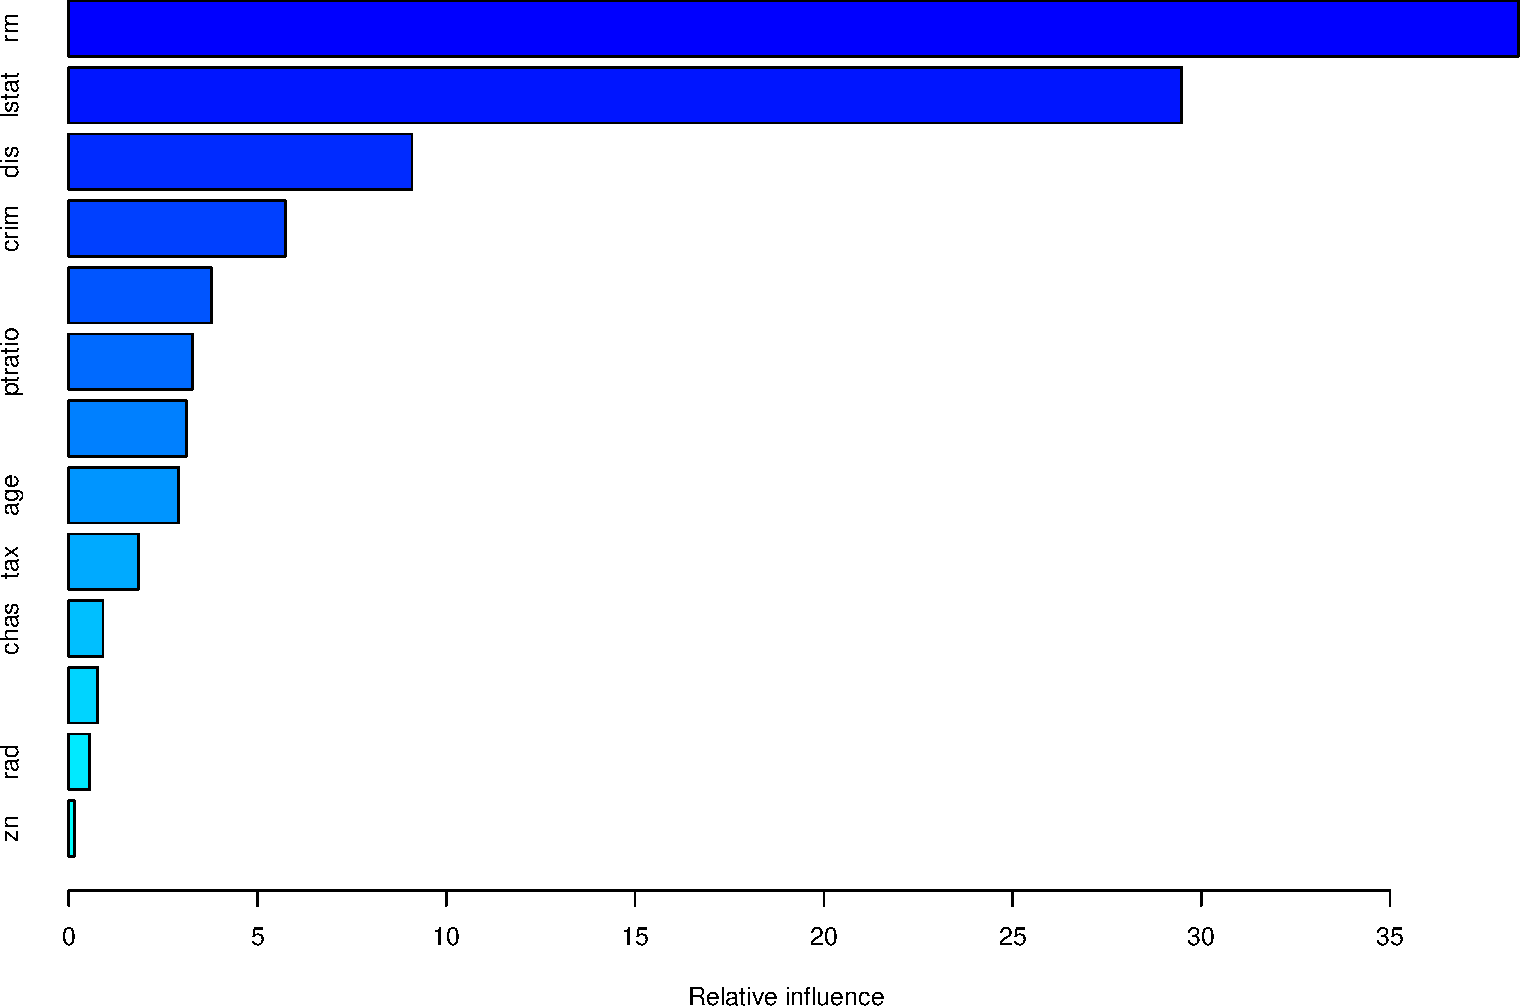
\includegraphics{EksploracjaDanych_files/figure-latex/unnamed-chunk-43-1.pdf}

\begin{verbatim}
##             var     rel.inf
## lstat     lstat 37.72235740
## rm           rm 28.25340805
## dis         dis  9.04378958
## crim       crim  6.95484787
## nox         nox  3.97210067
## black     black  3.16250916
## ptratio ptratio  3.03202030
## age         age  2.35790500
## chas       chas  1.97366108
## tax         tax  1.67544858
## indus     indus  1.22537648
## rad         rad  0.57329299
## zn           zn  0.05328283
\end{verbatim}

Predykcja na podstawie metody boosting

\begin{Shaded}
\begin{Highlighting}[]
\NormalTok{boston.pred4 <-}\StringTok{ }\KeywordTok{predict}\NormalTok{(boston.boost, }\DataTypeTok{newdata =}\NormalTok{ boston.test, }\DataTypeTok{n.trees =} \DecValTok{5000}\NormalTok{)}
\KeywordTok{rmse}\NormalTok{(boston.pred4, boston.test}\OperatorTok{$}\NormalTok{medv)}
\end{Highlighting}
\end{Shaded}

\begin{verbatim}
## [1] 3.06509
\end{verbatim}

\(RMSE\) jest w tym przypadku mniejsze niż w lasach losowych ale nieco większe niż w metodzie bagging. Wszystkie metody wzmacnianych drzew dają wyniki lepsze niż pojedyncze drzewa.

\hypertarget{klasyfikatory-liniowe}{%
\chapter{Klasyfikatory liniowe}\label{klasyfikatory-liniowe}}

Obszerną rodzinę klasyfikatorów stanowią modele liniowe (ang. \emph{linear classification models}). Klasyfikacji w tej rodzinie technik dokonuje się na podstawie modeli funkcji kombinacji liniowej predyktorów. Jest to ujęcie parametryczne, w którym klasyfikacji nowej wartości dokonujemy na podstawie atrybutów obserwacji i wektora parametrów. Uczenie na podstawie zestawu treningowego polega na oszacowaniu parametrów modelu. W odróżnieniu od metod nieparametrycznych postać modelu tym razem jest znana. Każdy klasyfikator liniowy skład się z funkcji wewnętrznej (ang. \emph{inner representation function}) i funkcji zewnętrznej (ang. \emph{outer representation function}).
Pierwsza jest funkcją rzeczywistą parametrów modelu i wartości atrybutów obserwacji
\begin{equation}
    g(x) = F(\mathbf{a}(x),\mathbf{w})=\sum_{i=0}^pw_ia_i(x)=\mathbf{w}\circ \mathbf{a}(x),
\end{equation}
przyjmując, że \(a_0(x)=1\).

Funkcja zewnętrzna przyporządkowuje binarnie klasy na podstawie wartości funkcji wewnętrznej. Istnieją dwa główne typy tych klasyfikacji:

\begin{itemize}
\tightlist
\item
  brzegowa - przyjmujemy, że funkcje wewnętrzne tworzą granice zbiorów obserwacji różnych klas,
\item
  probabilistyczna - bazująca na tym, że funkcje wewnętrzne mogą pośrednio wykazywać prawdopodobieństwo przynależności do danej klasy.
\end{itemize}

Pierwsza dzieli przestrzeń obserwacji za pomocą hiperpłaszczyzn na obszary jednorodne pod względem przynależności do klas. Druga jest próbą parametrycznej reprezentacji prawdopodobieństw przynależności do klas. Klasyfikacji na podstawie prawdopodobieństw można dokonać na różne sposoby, stosując:

\begin{itemize}
\tightlist
\item
  największe prawdopodobieństwo,
\item
  funkcję najmniejszego kosztu błędnej klasyfikacji,
\item
  krzywych ROC (ang. \emph{Receiver Operating Characteristic} - o tym później).
\end{itemize}

Podejście brzegowe lub probabilistyczne prowadzi najczęściej do dwóch typów reprezentacji funkcji zewnętrznej:

\begin{itemize}
\tightlist
\item
  reprezentacji progowej (ang. \emph{threshold representation}) - najczęściej przy podejściu brzegowym,
\item
  reprezentacji logistycznej (ang. \emph{logit representation}) - przy podejściu probabilistycznym.
\end{itemize}

\hypertarget{reprezentacja-progowa}{%
\section{Reprezentacja progowa}\label{reprezentacja-progowa}}

W przypadku klasyfikacji dwustanowej, dziedzina jest dzielona na dwa regiony (pozytywny i negatywny) poprzez porównanie funkcji zewnętrznej z wartością progową. Bez straty ogólności można sprawić, że będzie to wartość 0
\begin{equation}
    h(x)=H(g(x))= \begin{cases}
        1, &\text{ jeśli } g(x)\geq 0\\
        0, &\text{ w przeciwnym przypadku.}
    \end{cases}
\end{equation}
Czasami używa się parametryzacji \(\{-1,1\}\).
Przez porównanie \(g(x)\) z 0 definiuje się hiperpłaszczyznę w \(p\) wymiarowej przestrzeni, która rozdziela dziedzinę na regiony pozytywne i negatywne. W tym ujęciu mówimy o liniowej separowalności obserwacji różnych klas, jeśli istnieje hiperpłaszczyzna je rozdzielająca.

\hypertarget{reprezentacja-logitowa}{%
\section{Reprezentacja logitowa}\label{reprezentacja-logitowa}}

Najbardziej popularną reprezentacją parametryczną stosowaną w klasyfikacji jest reprezentacja logitowa
\begin{equation}
    \P(y=1|x)=\frac{e^{g(x)}}{e^{g(x)}+1}.
\end{equation}
Wówczas \(g(x)\) nie reprezentuje bezpośrednio \(\P(y=1|x)\) ale jego logit
\begin{equation}
    g(x)=\logit(\P(y=1|x)),
\end{equation}
gdzie \(\logit(p)=\ln\frac{p}{1-p}\). Dlatego właściwa postać reprezentacji jest następująca
\begin{equation}
    \P(y=1|x)=\logit^{-1}(g(x)).
\end{equation}
W ten sposób reprezentacja logitowa jest równoważna reprezentacji progowej, ponieważ
\begin{equation}
    g(x)=\ln\frac{\P(y=1|x)}{1-\P(y=1|x)}=\ln\frac{\P(y=1|x)}{\P(y=0|x)}>0.
\end{equation}
Jednak zaletą reprezentacji logitowej, w porównaniu do progowej, jest to, że można wyznaczyć prawdopodobieństwa przynależności do obu klas. W przypadku klasyfikacji wielostanowej uczymy tyle funkcji \(h\) ile jest klas.

\hypertarget{wady-klasyfikatorow-liniowych}{%
\section{Wady klasyfikatorów liniowych}\label{wady-klasyfikatorow-liniowych}}

\begin{itemize}
\tightlist
\item
  tylko w przypadku prostych funkcji wewnętrznych jesteśmy w stanie ocenić wpływ poszczególnych predykorów na klasyfikację,
\item
  jakość predykcji zależy od doboru funkcji wewnętrznej (liniowa w ścisłym sensie jest najczęściej niewystarczająca),
\item
  nie jest w stanie klasyfikować poprawnie stanów (nie jest liniowo separowalna) w zagadnieniach typu XOR.
\end{itemize}

\hypertarget{regresja-logistyczna}{%
\chapter{Regresja logistyczna}\label{regresja-logistyczna}}

\hypertarget{model-1}{%
\section{Model}\label{model-1}}

Regresja logistyczna (ang. \emph{logistic regression}) jest techniką z rodziny klasyfikatorów liniowych z reprezentacją logistyczną, a formalnie należy do rodziny uogólnionych modeli liniowych (GLM). Stosowana jest wówczas, gdy zmienna wynikowa posiada dwa stany (sukces i porażka), kodowane najczęściej za pomocą 1 i 0. W tej metodzie modelowane jest warunkowe prawdopodobieństwo sukcesu za pomocą kombinacji liniowej predyktorów \(X\).

Ogólna postać modelu
\begin{align}
    Y\sim &B(1, p)\\
    p(X)=&\E(Y|X)=\frac{\exp(\beta X)}{1+\exp(\beta X)},
\end{align}
gdzie \(B(1,p)\) jest rozkładem dwumianowym o prawdopodobieństwie sukcesu \(p\), a \(\beta X\) oznacza kombinację liniową parametrów modelu i wartości zmiennych niezależnych, przyjmując, że \(x_0=1\). Jako funkcji łączącej (czyli opisującej związek między kombinacją liniową predyktorów i prawdopodobieństwem sukcesu) użyto \emph{logitu}. Pozwala on na wygodną interpretację wyników w terminach szans.

Szansą (ang. \emph{odds}) nazywamy stosunek prawdopodobieństwa sukcesu do prawdopodobieństwa porażki
\begin{equation}
    o = \frac{p}{1-p}.
\end{equation}

Ponieważ będziemy przyjmowali, że \(p\in (0,1)\), to \(o\in (0,\infty)\), a jej logarytm należy do przedziału \((-\infty, \infty)\).

Zatem logarytm szansy jest kombinacją liniową predyktorów
\begin{equation}
    \log\left[\frac{p(X)}{1-p(X)}\right]=\beta_0+\beta_1x_1+\ldots+\beta_dx_d.
\end{equation}

\hypertarget{estymacja-parametrow-modelu}{%
\section{Estymacja parametrów modelu}\label{estymacja-parametrow-modelu}}

Estymacji parametrów modelu logistycznego dokonujemy za pomocą metody największej wiarogodności. Funkcja wiarogodności w tym przypadku przyjmuje postać
\begin{equation}
    L(X_1,\ldots,X_n,\beta)=\prod_{i=1}^{n}p(X_i)^Y_i[1-p(X_i)]^{1-Y_i},
\end{equation}
gdzie wektor \(\beta\) jest uwikłany w funkcji \(p(X_i)\). Maksymalizacji dokonujemy raczej po nałożeniu na funkcję wiarogodności logarytmu, bo to ułatwia szukanie ekstremum.
\begin{equation}
    \log L(X_1,\ldots,X_n,\beta) = \sum_{i=1}^n(Y_i\log p(X_i)+(1-Y_i)\log(1-p(X_i))).
\end{equation}

\hypertarget{interpretacja}{%
\section{Interpretacja}\label{interpretacja}}

Interpretacja (lat. \emph{ceteris paribus} - ``inne takie samo'') poszczególnych parametrów modelu jest następująca:

\begin{itemize}
\tightlist
\item
  jeśli \(b_i>0\) - to zmienna \(x_i\) ma wpływ stymulujący pojawienie się sukcesu,
\item
  jeśli \(b_i<0\) - to zmienna \(x_i\) ma wpływ ograniczający pojawienie się sukcesu,
\item
  jeśli \(b_i=0\) - to zmienna \(x_i\) nie ma wpływu na pojawienie się sukcesu.
\end{itemize}

Iloraz szans (ang. \emph{odds ratio}) stosuje się w przypadku porównywania dwóch klas obserwacji. Jest on jak sama nazwa wskazuje ilorazem szans zajścia sukcesu w obu klasach
\begin{equation}
    OR = \frac{p_1}{1-p_1}\frac{1-p_2}{p_2},
\end{equation}
gdzie \(p_i\) oznacza zajście sukcesu w \(i\)-tej klasie.

Interpretujemy go następująco:

\begin{itemize}
\tightlist
\item
  jeśli \(OR>1\) - to w pierwszej grupie zajście sukcesu jest bardziej prawdopodobne,
\item
  jeśli \(OR<1\) - to w drugiej grupie zajście sukcesu jest bardziej prawdopodobne,
\item
  jeśli \(OR=1\) - to w obu grupach zajście sukcesu jest jednakowo prawdopodobne.
\end{itemize}

\BeginKnitrBlock{example}
\protect\hypertarget{exm:logit}{}{\label{exm:logit} }Jako ilustrację działania regresji logistycznej użyjemy modelu dla danych ze zbioru \texttt{Default} pakietu \texttt{ISLR}.
\EndKnitrBlock{example}

\begin{Shaded}
\begin{Highlighting}[]
\KeywordTok{library}\NormalTok{(ISLR)}
\KeywordTok{head}\NormalTok{(Default)}
\end{Highlighting}
\end{Shaded}

\begin{verbatim}
##   default student   balance    income
## 1      No      No  729.5265 44361.625
## 2      No     Yes  817.1804 12106.135
## 3      No      No 1073.5492 31767.139
## 4      No      No  529.2506 35704.494
## 5      No      No  785.6559 38463.496
## 6      No     Yes  919.5885  7491.559
\end{verbatim}

Zmienną zależną jest \texttt{default}, a pozostałe są predyktorami. najpierw dokonamy podziału próby na ucząca i testową, a następnie zbudujemy model.

\begin{Shaded}
\begin{Highlighting}[]
\KeywordTok{set.seed}\NormalTok{(}\DecValTok{2019}\NormalTok{)}
\NormalTok{ind <-}\StringTok{ }\KeywordTok{sample}\NormalTok{(}\DecValTok{1}\OperatorTok{:}\KeywordTok{nrow}\NormalTok{(Default), }\DataTypeTok{size =} \DecValTok{2}\OperatorTok{/}\DecValTok{3}\OperatorTok{*}\KeywordTok{nrow}\NormalTok{(Default))}
\NormalTok{dt.ucz <-}\StringTok{ }\NormalTok{Default[ind,]}
\NormalTok{dt.test <-}\StringTok{ }\NormalTok{Default[}\OperatorTok{-}\NormalTok{ind,]}
\NormalTok{mod.logit <-}\StringTok{ }\KeywordTok{glm}\NormalTok{(default}\OperatorTok{~}\NormalTok{., dt.ucz, }\DataTypeTok{family =} \KeywordTok{binomial}\NormalTok{(}\StringTok{"logit"}\NormalTok{))}
\KeywordTok{summary}\NormalTok{(mod.logit)}
\end{Highlighting}
\end{Shaded}

\begin{verbatim}
## 
## Call:
## glm(formula = default ~ ., family = binomial("logit"), data = dt.ucz)
## 
## Deviance Residuals: 
##     Min       1Q   Median       3Q      Max  
## -2.4481  -0.1470  -0.0597  -0.0226   3.6966  
## 
## Coefficients:
##               Estimate Std. Error z value Pr(>|z|)    
## (Intercept) -1.085e+01  5.896e-01 -18.409   <2e-16 ***
## studentYes  -4.970e-01  2.851e-01  -1.744   0.0812 .  
## balance      5.604e-03  2.809e-04  19.949   <2e-16 ***
## income       7.933e-06  9.652e-06   0.822   0.4112    
## ---
## Signif. codes:  0 '***' 0.001 '**' 0.01 '*' 0.05 '.' 0.1 ' ' 1
## 
## (Dispersion parameter for binomial family taken to be 1)
## 
##     Null deviance: 1906.5  on 6665  degrees of freedom
## Residual deviance: 1059.8  on 6662  degrees of freedom
## AIC: 1067.8
## 
## Number of Fisher Scoring iterations: 8
\end{verbatim}

Tylko \texttt{income} nie ma żadnego wpływu na prawdopodobieństwo stanu \texttt{Yes} zmiennej \texttt{default}. Zmienna \texttt{balance} wpływa stymulująco na prawdopodobieństwo pojawienia się sukcesu. Natomiast jeśli badana osoba jest studentem (\texttt{studentYes}), to ma wpływ ograniczający na pojawienie się sukcesu. Chcąc porównać dwie grupy obserwacji, przykładowo studentów z nie-studentami, możemy wykorzystać iloraz szans.

\begin{Shaded}
\begin{Highlighting}[]
\KeywordTok{exp}\NormalTok{(}\KeywordTok{cbind}\NormalTok{(}\DataTypeTok{OR =} \KeywordTok{coef}\NormalTok{(mod.logit), }\KeywordTok{confint}\NormalTok{(mod.logit))) }\OperatorTok\StringTok{ }
\StringTok{    }\KeywordTok{kable}\NormalTok{(}\DataTypeTok{digits =} \DecValTok{4}\NormalTok{)}
\end{Highlighting}
\end{Shaded}

\begin{tabular}{l|r|r|r}
\hline
  & OR & 2.5 \% & 97.5 \%\\
\hline
(Intercept) & 0.0000 & 0.0000 & 0.0001\\
\hline
studentYes & 0.6083 & 0.3485 & 1.0668\\
\hline
balance & 1.0056 & 1.0051 & 1.0062\\
\hline
income & 1.0000 & 1.0000 & 1.0000\\
\hline
\end{tabular}

Z powyższej tabeli wynika, że bycie studentem zmniejsza szanse na \texttt{Yes} w zmiennej \texttt{default} o około 40\% (w stosunku do nie-studentów). Natomiast wzrost zmiennej \texttt{balance} przy zachowaniu pozostałych zmiennych na tym samym poziomie skutkuje wzrostem szans na \texttt{Yes} o około 0.6\%.

Chcąc przeprowadzić predykcję na podstawie modelu dla ustalonych wartości cech (np. \texttt{student\ =\ Yes}, \texttt{balance\ =\ \$1000} i \texttt{income\ =\ \$40000}) postępujemy następująco

\begin{Shaded}
\begin{Highlighting}[]
\NormalTok{dt.new <-}\StringTok{ }\KeywordTok{data.frame}\NormalTok{(}\DataTypeTok{student =} \StringTok{"Yes"}\NormalTok{, }\DataTypeTok{balance =} \DecValTok{1000}\NormalTok{, }\DataTypeTok{income =} \DecValTok{40000}\NormalTok{)}
\KeywordTok{predict}\NormalTok{(mod.logit, }\DataTypeTok{newdata =}\NormalTok{ dt.new, }\DataTypeTok{type =} \StringTok{"response"}\NormalTok{)}
\end{Highlighting}
\end{Shaded}

\begin{verbatim}
##           1 
## 0.004367692
\end{verbatim}

Otrzymany wynik jest oszacowanym prawdopodobieństwem warunkowym wystąpienia sukcesu (\texttt{default\ =\ Yes}). Widać zatem, że poziomy badanych cech sprzyjają raczej porażce.

Jeśli chcemy sprawdzić jakość klasyfikacji na zbiorze testowym, to musimy ustalić na jakim poziomie prawdopodobieństwa będziemy uznawać obserwację za sukces. W zależności od tego, na predykcji jakiego stanu zależy nam bardziej, możemy różnie dobierać ten próg (bez żadnych dodatkowych przesłanek najczęściej jest to 0.5).

\begin{Shaded}
\begin{Highlighting}[]
\NormalTok{pred <-}\StringTok{ }\KeywordTok{predict}\NormalTok{(mod.logit, }\DataTypeTok{newdata =}\NormalTok{ dt.test, }\DataTypeTok{type =} \StringTok{"response"}\NormalTok{)}
\NormalTok{pred.class <-}\StringTok{ }\KeywordTok{ifelse}\NormalTok{(pred }\OperatorTok{>}\StringTok{ }\FloatTok{0.5}\NormalTok{, }\StringTok{"Yes"}\NormalTok{, }\StringTok{"No"}\NormalTok{)}
\NormalTok{(tab <-}\StringTok{ }\KeywordTok{table}\NormalTok{(pred.class, dt.test}\OperatorTok{$}\NormalTok{default))}
\end{Highlighting}
\end{Shaded}

\begin{verbatim}
##           
## pred.class   No  Yes
##        No  3204   76
##        Yes   13   41
\end{verbatim}

\begin{Shaded}
\begin{Highlighting}[]
\NormalTok{(acc <-}\StringTok{ }\KeywordTok{sum}\NormalTok{(}\KeywordTok{diag}\NormalTok{(}\KeywordTok{prop.table}\NormalTok{(tab))))}
\end{Highlighting}
\end{Shaded}

\begin{verbatim}
## [1] 0.9733053
\end{verbatim}

Klasyfikacja na poziomie 97\% wskazuje na dobre dopasowanie modelu.

\hypertarget{LDA}{%
\chapter{Analiza dyskryminacyjna}\label{LDA}}

Analiza dyskryminacyjna (ang. \emph{discriminant analysis}) jest grupą technik dyskryminacji obserwacji względem przynależności do klas. Część z nich należy do klasyfikatorów liniowych (choć nie zawsze w ścisłym sensie). Za autorów tej metody uważa się Fisher'a (\protect\hyperlink{ref-fisher1936}{1936}) i Welch'a (\protect\hyperlink{ref-welch1939}{1939}). Każdy z nich prezentował nieco inne podejście do tematu klasyfikacji. Welch poszukiwał klasyfikacji minimalizującej prawdopodobieństwo błędnej klasyfikacji, znane jako \protect\hyperlink{bayes}{klasyfikatory bayesowskie}. Podejście Fisher'a skupiało się raczej na porównaniu zmienności międzygrupowej do zmienności wewnątrzgrupowej. Wychodząc z założenia, że iloraz tych wariancji powinien być stosunkowo duży przy różnych klasach, jeśli do ich opisu użyjemy odpowiednich zmiennych niezależnych. W istocie chodzi o znalezienie takiego wektora, w kierunku którego wspomniany iloraz wariancji jest największy.

\hypertarget{liniowa-analiza-dyskryminacyjna-fishera}{%
\section{Liniowa analiza dyskryminacyjna Fisher'a}\label{liniowa-analiza-dyskryminacyjna-fishera}}

\hypertarget{dwie-kategorie-zmiennej-grupujacej}{%
\subsection{Dwie kategorie zmiennej grupującej}\label{dwie-kategorie-zmiennej-grupujacej}}

Niech \(\boldsymbol D\) będzie zbiorem zawierającym \(n\) punktów \(\{\boldsymbol x_i, y_i\}\), gdzie \(\boldsymbol x_i\in \mathbb{R}^d\), a \(y_i\in \{c_1,\ldots,c_k\}\). Niech \(\boldsymbol D_i\) oznacza podzbiór punktów zbioru \(\boldsymbol D\), które należą do klasy \(c_i\), czyli \(\boldsymbol D_i=\{\boldsymbol x_i|y_i=c_i\}\) i niech \(|\boldsymbol D_i|=n_i\). Na początek załóżmy, że \(\boldsymbol D\) składa się tylko z \(\boldsymbol D_1\) i \(\boldsymbol D_2\).

Niech \(\boldsymbol w\) będzie wektorem jednostkowym (\(\boldsymbol w'\boldsymbol w=1\)), wówczas rzut ortogonalny punku \(\boldsymbol x_i\) na wektor \(\boldsymbol w\) można zapisać następująco
\begin{equation}
    \tilde{\boldsymbol x}_i=\left(\frac{\boldsymbol w'\boldsymbol x_i}{\boldsymbol w'\boldsymbol w}\right)\boldsymbol w=(\boldsymbol w'\boldsymbol x_i)\boldsymbol w = a_i\boldsymbol w,
\end{equation}
gdzie \(a_i\) jest współrzędną punktu \(\tilde{\boldsymbol x}_i\) w kierunku wektora \(\boldsymbol w\), czyli
\begin{equation}
    a_i=\boldsymbol w'\boldsymbol x_i.
\end{equation}
Zatem \((a_1,\ldots,a_n)\) reprezentują odwzorowanie \(\mathbb{R}^d\) w \(\mathbb{R}\), czyli z \(d\)-wymiarowej przestrzeni w przestrzeń generowaną przez \(\boldsymbol w\).

\begin{figure}

{\centering 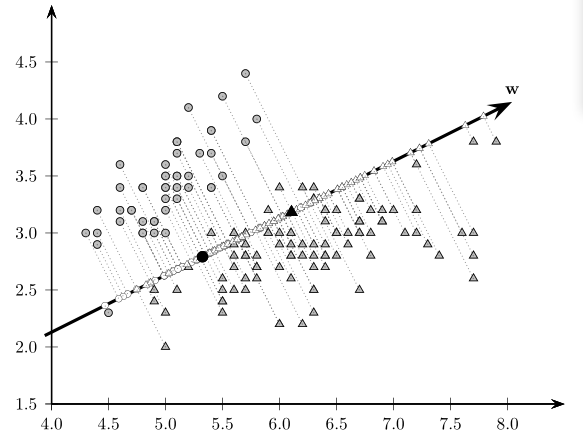
\includegraphics[width=5.83in]{images/rzut} 

}

\caption{Rzut ortogonalny punktów w kierunku wektora $\boldsymbol w$}\label{fig:rzut}
\end{figure}

Każdy punkt należy do pewnej klasy, dlatego możemy wyliczyć
\begin{align}
    m_1=&\frac{1}{n_1}\sum_{ \boldsymbol x_i\in \boldsymbol D_1}a_i=\\
    =&\frac{1}{n_1}\sum_{ \boldsymbol x_i\in \boldsymbol D_1} \boldsymbol w' \boldsymbol x_i=\\
    =& \boldsymbol w'\left(\frac{1}{n_1}\sum_{ \boldsymbol x_i\in \boldsymbol D_1} \boldsymbol x_i \right)=\\
    =& \boldsymbol w' \boldsymbol{\mu}_1,
    \label{eq:m}
\end{align}
gdzie \(\boldsymbol \mu_1\) jest wektorem średnich punktów z \(\boldsymbol D_1\). W podobny sposób można policzyć \(m_2 = \boldsymbol w' \boldsymbol \mu_2\). Oznacza to, że średnia projekcji jest projekcją średnich.

Rozsądnym wydaje się teraz poszukać takiego wektora, aby \(|m_1-m_2|\) była maksymalnie duża przy zachowaniu niezbyt dużej zmienności wewnątrz grup. Dlatego kryterium Fisher'a przyjmuje postać
\begin{equation}
    \max_{ \boldsymbol w}J(\boldsymbol w)=\frac{(m_1-M_2)^2}{ss_1^2+ss_2^2},
    \label{eq:condFisher}
\end{equation}
gdzie \(ss_j^2=\sum_{ \boldsymbol x_i\in \boldsymbol D_j}(a_i-m_j)^2=n_j\sigma_j^2.\)

Zauważmy, że licznik w \eqref{eq:condFisher} da się zapisać jako
\begin{align}
    (m_1-m_2)^2=& ( \boldsymbol w'( \boldsymbol \mu_1- \boldsymbol \mu_2))^2=\\
    =& \boldsymbol w'((\boldsymbol \mu_1- \boldsymbol \mu_2)(\boldsymbol \mu_1- \boldsymbol \mu_2)') \boldsymbol w=\\
    =& \boldsymbol w' \boldsymbol B \boldsymbol w
\end{align}
gdzie \(\boldsymbol B=(\boldsymbol \mu_1- \boldsymbol \mu_2)(\boldsymbol \mu_1- \boldsymbol \mu_2)'\) jest macierzą \(d\times d\).

Ponadto
\begin{align}
    ss_j^2=&\sum_{ \boldsymbol x_i\in \boldsymbol D_j}(a_i-m_j)^2=\\
    =&\sum_{ \boldsymbol x_i\in \boldsymbol D_j}( \boldsymbol w' \boldsymbol x_i- \boldsymbol w' \boldsymbol\mu_j)^2=\\
    =& \sum_{ \boldsymbol x_i\in \boldsymbol D_j}( \boldsymbol{w}'( \boldsymbol{x}_i- \boldsymbol{\mu}_j))^2=\\
    =& \boldsymbol{w}'\left(\sum_{ \boldsymbol x_i\in \boldsymbol D_j}(\boldsymbol{x}_i-\boldsymbol \mu_j)(\boldsymbol x_i- \boldsymbol \mu_j)'\right) \boldsymbol{w}=\\
    =& \boldsymbol{w}' \boldsymbol{S}_j \boldsymbol{w},
    \label{eq:Sj}
\end{align}
gdzie \(\boldsymbol{S}_j=n_j \boldsymbol{\Sigma}_j\).
Zatem mianownik \eqref{eq:condFisher} możemy zapisać jako
\begin{equation}
    ss_1^2+ss_2^2= \boldsymbol{w}'(\boldsymbol{S}_1+ \boldsymbol{S}_2) \boldsymbol{w}= \boldsymbol{w}' \boldsymbol{S} \boldsymbol{w},
\end{equation}
gdzie \(\boldsymbol{S}=\boldsymbol{S}_1+\boldsymbol{S}_2\).
Ostatecznie warunek Fisher'a przyjmuje postać
\begin{equation}
    \max_{ \boldsymbol{w}}J( \boldsymbol{w})=\frac{ \boldsymbol{w}' \boldsymbol{B} \boldsymbol{w}}{ \boldsymbol{w}' \boldsymbol{S} \boldsymbol{w}}.
    \label{eq:condFisher2}
\end{equation}

Różniczkując \eqref{eq:condFisher2} po \(\boldsymbol{w}\) otrzymamy warunek
\begin{equation}
    \boldsymbol{B} \boldsymbol{w} = \lambda \boldsymbol{S} \boldsymbol{w},
    \label{eq:condFisher3}
\end{equation}
gdzie \(\lambda=J(\boldsymbol{w})\). Maksimum \eqref{eq:condFisher3} jest osiągane dla wektora \(\boldsymbol{w}\) równego wektorowi własnemu odpowiadającemu największej wartości własnej równania charakterystycznego \(|\boldsymbol{B}-\lambda\boldsymbol{S}|=0\). Jeśli \(\boldsymbol{S}\) nie jest osobliwa, to rozwiązanie \eqref{eq:condFisher3} otrzymujemy przez znalezienie największej wartości własnej macierzy \(\boldsymbol{B}\boldsymbol{S}^{-1}\) lub bez wykorzystania wartości i wektorów własnych.

Ponieważ \(\boldsymbol{B}=\left((\boldsymbol{\mu}_1-\boldsymbol{\mu}_2)(\boldsymbol{\mu}_1-\boldsymbol{\mu}_2)'\right)\boldsymbol{w}\) jest macierzą \(d \times d\) rzędu 1, to \(\boldsymbol{B}\boldsymbol{w}\) jest punktem na kierunku wyznaczonym przez wektor \(\boldsymbol{\mu}_1-\boldsymbol{\mu}_2\), bo
\begin{align}
    \boldsymbol{B}\boldsymbol{w}=& \left((\boldsymbol{\mu}_1-\boldsymbol{\mu}_2)(\boldsymbol{\mu}_1-\boldsymbol{\mu}_2)'\right)\boldsymbol{w}=\\
    =&(\boldsymbol{\mu}_1-\boldsymbol{\mu}_2)\left((\boldsymbol{\mu}_1-\boldsymbol{\mu}_2)'\right)\boldsymbol{w}=\\
    =& b(\boldsymbol{\mu}_1-\boldsymbol{\mu}_2),
\end{align}
gdzie \(b = (\boldsymbol{\mu}_1-\boldsymbol{\mu}_2)'\boldsymbol{w}\) jest skalarem.

Wówczas \eqref{eq:condFisher3} zapiszemy jako
\begin{gather}
    b(\boldsymbol{\mu}_1-\boldsymbol{\mu}_2) = \lambda\boldsymbol{S}\boldsymbol{w}\\
    \boldsymbol{w}= \frac{b}{\lambda}\boldsymbol{S}^{-1}(\boldsymbol{\mu}_1-\boldsymbol{\mu}_2)
\end{gather}

A ponieważ \(b/\lambda\) jest liczbą, to kierunek najlepszej dyskryminacji grup wyznacza wektor
\begin{equation}
    \boldsymbol{w}=\boldsymbol{S}^{-1}(\boldsymbol{\mu}_1-\boldsymbol{\mu}_2).
\end{equation}

\begin{figure}

{\centering 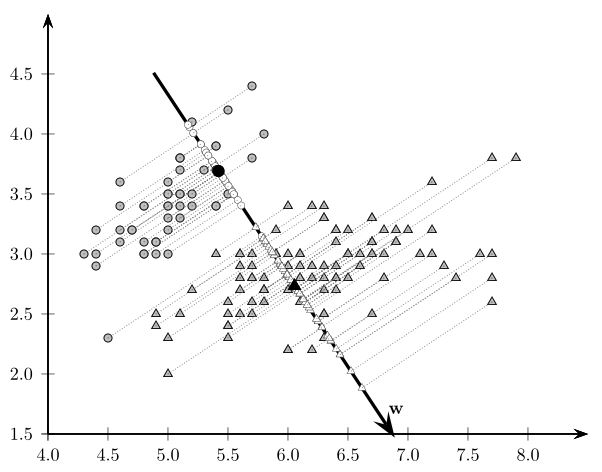
\includegraphics{images/rzut2} 

}

\caption{Rzut ortogonalny w kierunku wektora $\boldsymbol{w}$, będącego najlepiej dyskryminującym obie grupy obserwacji}\label{fig:rzut2}
\end{figure}

\hypertarget{k-kategorii-zmiennej-grupujacej}{%
\subsection{\texorpdfstring{\(k\)-kategorii zmiennej grupującej}{k-kategorii zmiennej grupującej}}\label{k-kategorii-zmiennej-grupujacej}}

Uogólnieniem tej teorii na przypadek \(k\) klas otrzymujemy przez uwzględnienie \(k-1\) funkcji dyskryminacyjnych. Zmienność wewnątrzgrupowa przyjmuje wówczas postać
\begin{equation}
    \boldsymbol{S}_W=\sum_{i=1}^k\boldsymbol{S}_i,
\end{equation}
gdzie \(\boldsymbol{S}_i\) jest zdefiniowane jak w \eqref{eq:Sj}.
Niech średnia i rozrzut globalny będą dane wzorami
\begin{equation}
    \boldsymbol{m}=\frac{1}{n}\sum_{i=1}^kn_i\boldsymbol{m}_i,
\end{equation}
\begin{equation}
    \boldsymbol{S}_T=\sum_{j=1}^k\sum_{\boldsymbol{x}\in D_j}(\boldsymbol{x}-\boldsymbol{m})(\boldsymbol{x}-\boldsymbol{m})'
\end{equation}
gdzie \(\boldsymbol{m}_i\) jest określone jak w \eqref{eq:m}. Wtedy zmienność międzygrupową możemy wyrazić jako
\begin{equation}
    \boldsymbol{S}_B=\sum_{i=1}^kn_i(\boldsymbol{m}_i-\boldsymbol{m})(\boldsymbol{m}_i-\boldsymbol{m})',
\end{equation}
bo \(\boldsymbol{S}_T=\boldsymbol{S}_W+\boldsymbol{S}_B.\)
Określamy projekcję \(d\)-wymiarowej przestrzeni na \(k-1\)-wymiarową przestrzeń za pomocą \(k-1\) funkcji dyskryminacyjnych postaci
\begin{equation}
    \boldsymbol{a}_j=\boldsymbol{w}_j'\boldsymbol{x}, \quad j=1,\ldots,k-1.
\end{equation}
Połączone wszystkie \(k-1\) rzutów możemy zapisać jako
\begin{equation}
    \boldsymbol{a}=\boldsymbol{W}'\boldsymbol{x}.
\end{equation}

W nowej przestrzeni \(k-1\)-wymiarowej możemy zdefiniować
\begin{equation}
    \tilde{\boldsymbol{m}}=\frac{1}{n}\sum_{i=1}^kn_i\tilde{\boldsymbol{m}}_i,
\end{equation}
gdzie \(\tilde{\boldsymbol{m}}_i= \frac{1}{n_i}\sum_{\boldsymbol{a}\in A_i}\boldsymbol{a}\), a \(A_i\) jest projekcją obiektów z \(i\)-tej klasy w kierunku wektora \(\boldsymbol{W}\).
Dalej możemy zdefiniować zmienności miedzy- i wewnątrzgrupowe dla obiektów przekształconych przez \(\boldsymbol{W}\)
\begin{align}
    \tilde{\boldsymbol{S}}_W=&\sum_{i=1}^k\sum_{\boldsymbol{a}\in A_i}(\boldsymbol{a}-\tilde{\boldsymbol{m}})(\boldsymbol{a}-\tilde{\boldsymbol{m}})'\\
    \tilde{\boldsymbol{S}}_B=&\sum_{i=1}^kn_i(\tilde{\boldsymbol{m}}_i-\tilde{\boldsymbol{m}})(\tilde{\boldsymbol{m}}_i-\tilde{\boldsymbol{m}})'.
\end{align}
Łatwo można zatem pokazać, że
\begin{align}
    \tilde{\boldsymbol{S}}_W = & \boldsymbol{W}'\boldsymbol{S}_W\boldsymbol{W}\\
    \tilde{\boldsymbol{S}}_B = & \boldsymbol{W}'\boldsymbol{S}_B\boldsymbol{W}.
\end{align}
Ostatecznie warunek \eqref{eq:condFisher} w \(k\)-wymiarowym ujęciu można przedstawić jako
\begin{equation}
    \max_{\boldsymbol{W}}J(\boldsymbol{W})=\frac{\tilde{\boldsymbol{S}}_W}{\tilde{\boldsymbol{S}}_B}=\frac{\boldsymbol{W}'\boldsymbol{S}_W\boldsymbol{W}}{\boldsymbol{W}'\boldsymbol{S}_B\boldsymbol{W}}.
\end{equation}
Maksimum można znaleźć poprzez rozwiązanie równania charakterystycznego \begin{equation}
    |\boldsymbol{S}_B-\lambda_i\boldsymbol{S}_W|=0
\end{equation}
dla każdego \(i\).

\BeginKnitrBlock{example}
\protect\hypertarget{exm:unnamed-chunk-51}{}{\label{exm:unnamed-chunk-51} }Dla danych ze zbioru \texttt{iris} przeprowadzimy analizę dyskryminacji. Implementację metody LDA znajdziemy w pakiecie \texttt{MASS} w postaci funkcji \texttt{lda}.
\EndKnitrBlock{example}

Zaczynamy od standaryzacji zmiennych i podziału próby na uczącą i testową.

\begin{Shaded}
\begin{Highlighting}[]
\KeywordTok{library}\NormalTok{(MASS)}
\KeywordTok{library}\NormalTok{(tidyverse)}
\NormalTok{iris.std <-}\StringTok{ }\NormalTok{iris }\OperatorTok\StringTok{ }
\StringTok{    }\KeywordTok{mutate_if}\NormalTok{(is.numeric, scale)}
\KeywordTok{set.seed}\NormalTok{(}\DecValTok{2019}\NormalTok{)}
\NormalTok{ind <-}\StringTok{ }\KeywordTok{sample}\NormalTok{(}\KeywordTok{nrow}\NormalTok{(iris.std), }\DataTypeTok{size =} \DecValTok{100}\NormalTok{)}
\NormalTok{dt.ucz <-}\StringTok{ }\NormalTok{iris.std[ind,]}
\NormalTok{dt.test <-}\StringTok{ }\NormalTok{iris.std[}\OperatorTok{-}\NormalTok{ind,]}
\end{Highlighting}
\end{Shaded}

Budowa modelu

\begin{Shaded}
\begin{Highlighting}[]
\NormalTok{mod.lda <-}\StringTok{ }\KeywordTok{lda}\NormalTok{(Species}\OperatorTok{~}\NormalTok{., }\DataTypeTok{data =}\NormalTok{ dt.ucz)}
\NormalTok{mod.lda}\OperatorTok{$}\NormalTok{prior}
\end{Highlighting}
\end{Shaded}

\begin{verbatim}
##     setosa versicolor  virginica 
##       0.36       0.31       0.33
\end{verbatim}

Prawdopodobieństwa \emph{a priori} przynależności do klas przyjęto na podstawie próby uczącej.

\begin{Shaded}
\begin{Highlighting}[]
\NormalTok{mod.lda}\OperatorTok{$}\NormalTok{means}
\end{Highlighting}
\end{Shaded}

\begin{verbatim}
##            Sepal.Length Sepal.Width Petal.Length Petal.Width
## setosa       -1.0251463   0.8690229    -1.294839  -1.2527443
## versicolor    0.1619267  -0.5015842     0.316167   0.1786195
## virginica     0.9174351  -0.2636338     1.046883   1.0504160
\end{verbatim}

W części \texttt{means} wyświetlone są średnie poszczególnych zmiennych niezależnych w podziale na grupy. Dzięki temu można określić położenia środków ciężkości poszczególnych klas w oryginalnej przestrzeni.

\begin{Shaded}
\begin{Highlighting}[]
\NormalTok{mod.lda}\OperatorTok{$}\NormalTok{scaling}
\end{Highlighting}
\end{Shaded}

\begin{verbatim}
##                     LD1       LD2
## Sepal.Length  1.0073378  0.211252
## Sepal.Width   0.4701094 -1.053135
## Petal.Length -4.0746585  1.488372
## Petal.Width  -2.5146178 -2.312201
\end{verbatim}

Powyższa tabela zawiera współrzędne wektorów wyznaczających funkcje dyskryminacyjne. Na ich podstawie możemy określić, która z nich wpływa najmocniej na tworzenie się nowej przestrzeni.

Obiekt \texttt{svd} przechowuje pierwiastki z \(\lambda_i\), dlatego podnosząc je do kwadratu i dzieląc przez ich sumę otrzymamy udział poszczególnych zmiennych w dyskryminacji przypadków. Jak widać pierwsza funkcja dyskryminacyjna w zupełności by wystarczyła.

\begin{Shaded}
\begin{Highlighting}[]
\NormalTok{mod.lda}\OperatorTok{$}\NormalTok{svd}\OperatorTok{^}\DecValTok{2}\OperatorTok{/}\KeywordTok{sum}\NormalTok{(mod.lda}\OperatorTok{$}\NormalTok{svd}\OperatorTok{^}\DecValTok{2}\NormalTok{)}
\end{Highlighting}
\end{Shaded}

\begin{verbatim}
## [1] 0.994875091 0.005124909
\end{verbatim}

Klasyfikacja na podstawie modelu

\begin{Shaded}
\begin{Highlighting}[]
\NormalTok{pred.lda <-}\StringTok{ }\KeywordTok{predict}\NormalTok{(mod.lda, dt.test)}
\end{Highlighting}
\end{Shaded}

Wynik predykcji przechowuje trzy rodzaje obiektów:

\begin{itemize}
\tightlist
\item
  klasy, które przypisał obiektom model (\texttt{class});
\item
  prawdopodobieństwa \emph{a posteriori} przynależności do klas na podstawie modelu (\texttt{posterior});
\item
  współrzędne w nowej przestrzeni LD1, LD2 (\texttt{x}).
\end{itemize}

Sprawdzenie jakości klasyfikacji

\begin{Shaded}
\begin{Highlighting}[]
\NormalTok{tab <-}\StringTok{ }\KeywordTok{table}\NormalTok{(}\DataTypeTok{pred =}\NormalTok{ pred.lda}\OperatorTok{$}\NormalTok{class, }\DataTypeTok{obs =}\NormalTok{ dt.test}\OperatorTok{$}\NormalTok{Species)}
\NormalTok{tab}
\end{Highlighting}
\end{Shaded}

\begin{verbatim}
##             obs
## pred         setosa versicolor virginica
##   setosa         14          0         0
##   versicolor      0         18         0
##   virginica       0          1        17
\end{verbatim}

\begin{Shaded}
\begin{Highlighting}[]
\KeywordTok{sum}\NormalTok{(}\KeywordTok{diag}\NormalTok{(}\KeywordTok{prop.table}\NormalTok{(tab)))}
\end{Highlighting}
\end{Shaded}

\begin{verbatim}
## [1] 0.98
\end{verbatim}

Jak widać z powyższej tabeli model dobrze sobie radzi z klasyfikacją obiektów. Odsetek poprawnych klasyfikacji wynosi 98\%.

\begin{Shaded}
\begin{Highlighting}[]
\KeywordTok{cbind.data.frame}\NormalTok{(}\DataTypeTok{obs =}\NormalTok{ dt.test}\OperatorTok{$}\NormalTok{Species,}
\NormalTok{                 pred.lda}\OperatorTok{$}\NormalTok{x, }
                 \DataTypeTok{pred =}\NormalTok{ pred.lda}\OperatorTok{$}\NormalTok{class) }\OperatorTok\StringTok{ }
\StringTok{    }\KeywordTok{ggplot}\NormalTok{(}\KeywordTok{aes}\NormalTok{(}\DataTypeTok{x =}\NormalTok{ LD1, }\DataTypeTok{y =}\NormalTok{ LD2))}\OperatorTok{+}
\StringTok{    }\KeywordTok{geom_point}\NormalTok{(}\KeywordTok{aes}\NormalTok{(}\DataTypeTok{color =}\NormalTok{ pred, }\DataTypeTok{shape =}\NormalTok{ obs))}
\end{Highlighting}
\end{Shaded}

\begin{figure}

{\centering 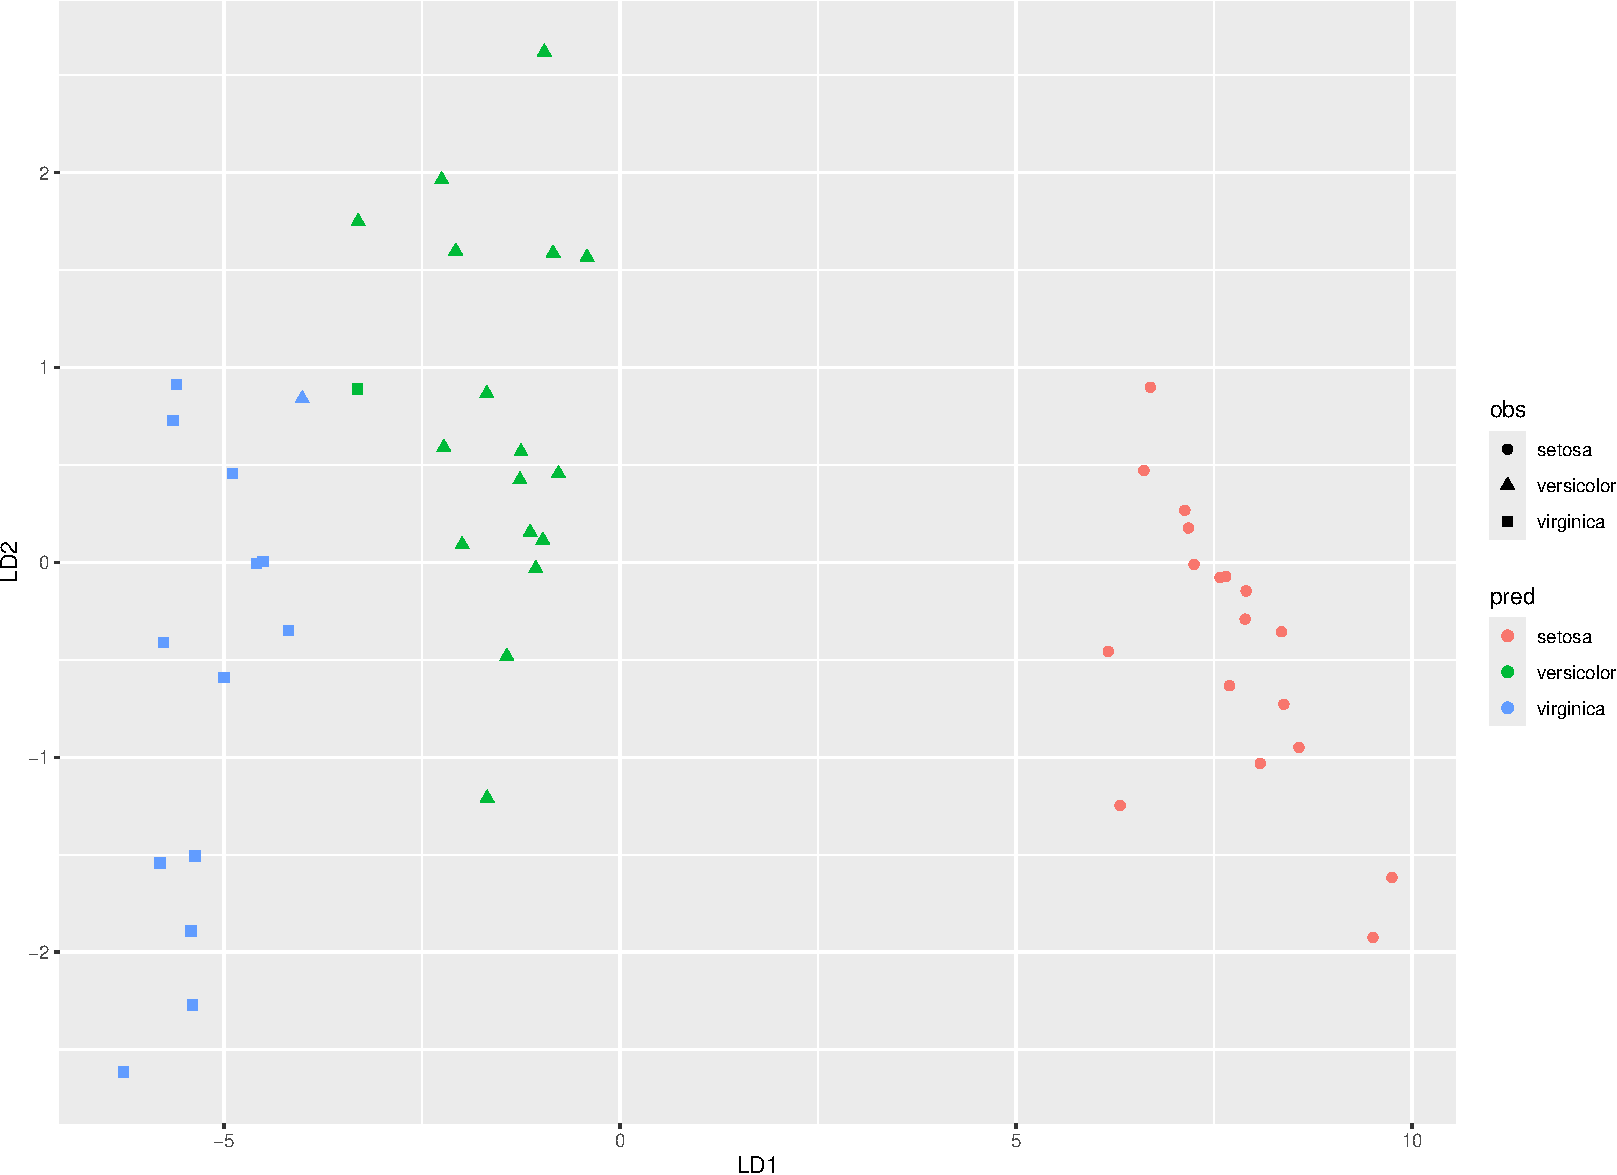
\includegraphics{EksploracjaDanych_files/figure-latex/unnamed-chunk-59-1} 

}

\caption{Klasyfikacja w przestrzeni LD1, LD2 na podstawie modelu mod.lda}\label{fig:unnamed-chunk-59}
\end{figure}

\hypertarget{liniowa-analiza-dyskryminacyjna---podejscie-probabilistyczne}{%
\section{Liniowa analiza dyskryminacyjna - podejście probabilistyczne}\label{liniowa-analiza-dyskryminacyjna---podejscie-probabilistyczne}}

Jak wspomniano na wstępie (patrz rozdział \ref{LDA}), podejście prezentowane przez Welcha polegało na minimalizacji prawdopodobieństwa popełnienia błędu przy klasyfikacji. Cała rodzina klasyfikatorów Bayesa (patrz rozdział \ref{bayes}) polega na wyznaczeniu prawdopodobieństw \emph{a posteriori}, na podstawie których dokonuje się decyzji o klasyfikacji obiektów. Tym razem dodajemy również założenie, że zmienne niezależne \(\boldsymbol{x}=(\boldsymbol{x}_1,\ldots,\boldsymbol{x}_d)\) charakteryzują się wielowymiarowym rozkładem normalnym
\begin{equation}
    f(\boldsymbol{x}) = \frac{1}{(2\pi)^{d/2}|\boldsymbol{\Sigma}|^{1/2}}\exp\left[-\frac{1}{2}(\boldsymbol{x}-\boldsymbol{\mu})'\boldsymbol{\Sigma}(\boldsymbol{x}-\boldsymbol{\mu})\right],
    \label{eq:mnv}
\end{equation}
gdzie \(\boldsymbol{\mu}\) jest wektorem średnich \(\boldsymbol{x}\), a \(\boldsymbol{\Sigma}\) jest macierzą kowariancji \(\boldsymbol{x}\).

\BeginKnitrBlock{remark}
\iffalse{} {Uwaga. } \fi{}Liniowa kombinacja zmiennych losowych o normalnym rozkładzie łącznym ma również rozkład łączny normalny. W szczególności, jeśli \(A\) jest macierzą wymiaru \(d\times k\) i \(\boldsymbol{y} = A'\boldsymbol{x}\), to \(f(\boldsymbol{y})\sim N(A'\boldsymbol{\mu}, A'\boldsymbol{\Sigma}A)\). Odpowiednia forma macierzy przekształcenia \(A_w\), sprawia, że zmienne po transformacji charakteryzują się rozkładem normalnym łącznym o wariancji określonej przez \(I\). Jeśli \(\boldsymbol{\Phi}\) jest macierzą, której kolumny są ortonormalnymi wektorami własnymi macierzy \(\boldsymbol{\Sigma}\), a \(\boldsymbol{\Lambda}\) macierzą diagonalną wartości własnych, to transformacja \(A_w=\boldsymbol{\Phi}\boldsymbol{\Lambda}^{-1}\) przekształca \(\boldsymbol{x}\) w \(\boldsymbol{y}\sim N(A_w'\boldsymbol{\mu}, I)\).
\EndKnitrBlock{remark}

\begin{figure}

{\centering 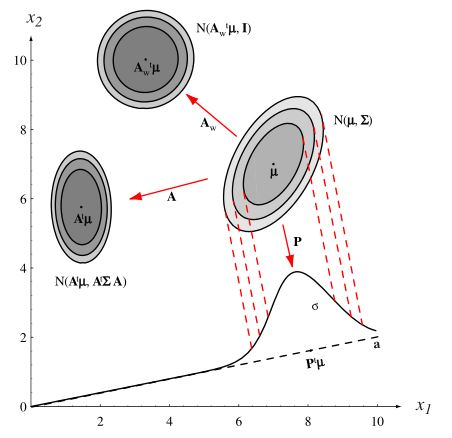
\includegraphics{images/transform} 

}

\caption{Transformacje rozkładu normalnego łącznego. Źródło: @duda2001}\label{fig:trans}
\end{figure}

\BeginKnitrBlock{definition}
\protect\hypertarget{def:unnamed-chunk-60}{}{\label{def:unnamed-chunk-60} }Niech \(g_i(\boldsymbol{x}),\ i=1,\ldots,k\) będzie pewną funkcją dyskryminacyjną, wówczas obiekt \(\boldsymbol{x}\) nalezy zaklasyfikować do grupy \(c_i\) jeśli spełniony jest warunek
\begin{equation}
    g_i(\boldsymbol{x})>g_j(\boldsymbol{x}), \quad j\neq i.
\end{equation}
\EndKnitrBlock{definition}

W podejściu polegającym na minimalizacji prawdopodobieństwa błędnej klasyfikacji, przyjmuje się najczęściej, że
\begin{equation}
    g_i(\boldsymbol{x})=\P(c_i|\boldsymbol{x}),
\end{equation}
czyli jako prawdopodobieństwo a posteriori.
Wszystkie trzy poniższe postaci funkcji dyskryminacyjnych są dopuszczalne i równoważne ze względu na rezultat grupowania
\begin{align}
    g_i(\boldsymbol{x})=&\P(c_i|\boldsymbol{x})=\frac{\P(\boldsymbol{x}|c_i)\P(c_i)}{\sum_{i=1}^k\P(\boldsymbol{x}|c_i)\P(c_i)},\\
    g_i(\boldsymbol{x})=&\P(\boldsymbol{x}|c_i)\P(c_i),\\
    g_i(\boldsymbol{x})=&\log\P(\boldsymbol{x}|c_i)+\log\P(c_i)
    \label{eq:gi3}
\end{align}
W przypadku gdy \(\boldsymbol{x}|c_i\sim N(\boldsymbol{\mu}_i, \boldsymbol{\Sigma}_i)\), to na podstawie \eqref{eq:mnv} \(g_i\) danej jako \eqref{eq:gi3} przyjmuje postać
\begin{equation}
    g_i(\boldsymbol{x})=-\frac{1}{2}(\boldsymbol{x}-\boldsymbol{\mu}_i)'\boldsymbol{\Sigma}_i^{-1}(\boldsymbol{x}-\boldsymbol{\mu}_i)-\frac{d}{2}\log(2\pi)-\frac{1}{2}\log|\boldsymbol{\Sigma}_i|+\log\P(c_i).
\end{equation}

W kolejnych podrozdziałach przeanalizujemy trzy możliwe formy macierzy kowariancji.

\hypertarget{przypI}{%
\subsection{\texorpdfstring{Przypadek gdy \(\boldsymbol{\Sigma}_i=\sigma^2I\)}{Przypadek gdy \textbackslash{}boldsymbol\{\textbackslash{}Sigma\}\_i=\textbackslash{}sigma\^{}2I}}\label{przypI}}

To najprostszy przypadek, zakładający niezależność zmiennych wchodzących w skład \(\boldsymbol x\), których wariancje są stałe \(\sigma^2\).
Wówczas \(g_i\) przyjmuje postać
\begin{equation}
    g_i(\boldsymbol x)=-\frac{||\boldsymbol x-\boldsymbol \mu_i||^2}{2\sigma^2}+\log\P(c_i),
    \label{eq:row88}
\end{equation}
gdzie \(||\cdot ||\) jest normą euklidesową.

Rozpisując licznik równania \eqref{eq:row88} mamy
\begin{equation}
    ||\boldsymbol x-\boldsymbol \mu_i||^2=(\boldsymbol x-\boldsymbol \mu_i)'(\boldsymbol x-\boldsymbol \mu_i).
\end{equation}
Zatem
\begin{equation}
    g_i(\boldsymbol x)=-\frac{1}{2\sigma^2}[\boldsymbol x'\boldsymbol x-2\boldsymbol \mu_i'\boldsymbol x+\boldsymbol \mu_i'\boldsymbol \mu_i]+\log\P(c_i).
\end{equation}
A ponieważ \(\boldsymbol x'\boldsymbol x\) nie zależy do \(i\), to funkcję dyskryminacyjną możemy zapisać jako
\begin{equation}
    g_i(\boldsymbol x)=\boldsymbol w_i'\boldsymbol x+w_{i0},
\end{equation}
gdzie \(\boldsymbol w_i=\frac{1}{\sigma^2}\boldsymbol \mu_i\), a \(w_{i0}=\frac{-1}{2\sigma^2}\boldsymbol \mu_i'\boldsymbol \mu_i+\log\P(c_i).\)

Na podstawie funkcji dyskryminacyjnych wyznaczamy hiperpłaszczyzny decyzyjne jako zbiory punktów dla których \(g_i(\boldsymbol x)=g_j(\boldsymbol x)\), gdzie \(g_i, g_j\) są największe. Możemy to zapisać w następujący sposób
\begin{equation}
    \boldsymbol w'(\boldsymbol x-\boldsymbol x_0)=0,
    \label{eq:row89}
\end{equation}
gdzie
\begin{equation}
    \boldsymbol w = \boldsymbol \mu_i-\boldsymbol \mu_j,
\end{equation}
oraz
\begin{equation}
    \boldsymbol x_0 = \frac12(\boldsymbol \mu_i+\boldsymbol\mu_j)-\frac{\sigma^2}{||\boldsymbol \mu_i-\boldsymbol \mu_j||^2}\log\frac{\P(c_i)}{\P(c_j)}(\boldsymbol \mu_i-\boldsymbol \mu_j).
\end{equation}

Równanie \eqref{eq:row89} określa hiperpłaszczyznę przechodzącą przez \(\boldsymbol x_0\) i prostopadłą do \(\boldsymbol w\).

\begin{figure}

{\centering 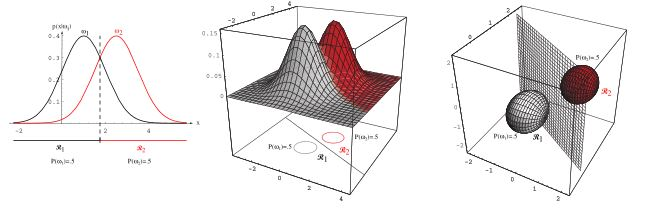
\includegraphics{images/dyskrym1} 

}

\caption{Dyskrymiancja hiperpłaszczyznami w sygucaji dwóch klas. Wykres po lewej, to ujęcie jednowymiarowe, wykresy po środu - ujęcie 2-wymiarowe i wykresy po prawej, to ujęcie 3-wymiarowe. Źródło: @duda2001}\label{fig:hiper}
\end{figure}

\hypertarget{przypSig}{%
\subsection{\texorpdfstring{Przypadek gdy \(\boldsymbol \Sigma_i=\boldsymbol \Sigma\)}{Przypadek gdy \textbackslash{}boldsymbol \textbackslash{}Sigma\_i=\textbackslash{}boldsymbol \textbackslash{}Sigma}}\label{przypSig}}

Przypadek ten opisuje sytuację, gdy rozkłady \(\boldsymbol x\) są identyczne we wszystkich grupach ale zmienne w ich skład wchodzące nie są niezależne.
W tym przypadku funkcje dyskryminacyjne przyjmują postać
\begin{equation}
    g_i(\boldsymbol x)=\frac12(\boldsymbol x-\boldsymbol \mu_i)'\boldsymbol\Sigma^{-1}(\boldsymbol x-\boldsymbol \mu_i)+\log\P(c_i).
    \label{eq:row810}
\end{equation}
Jeśli \(\P(c_i)\) są identyczne dla wszystkich klas, to można je pominąć we wzorze \eqref{eq:row810}. Metryka euklidesowa ze wzoru \eqref{eq:row88} została zastąpiona przez odległość Mahalonobis'a. Podobnie ja w przypadku gdy \(\boldsymbol \Sigma_i=\sigma^2I\), tak i teraz można uprościć \eqref{eq:row810} przez rozpisanie formy kwadratowej, aby otrzymać, że
\begin{equation}
    g_i(\boldsymbol x)=\boldsymbol w_i'\boldsymbol x+w_{i0},
\end{equation}
gdzie \(\boldsymbol w_i=\boldsymbol\Sigma^{-1}\boldsymbol \mu_i\), a \(w_{i0}=-\frac{1}{2}\boldsymbol \mu_i'\boldsymbol\Sigma^{-1}\boldsymbol \mu_i+\log\P(c_i).\)

Ponieważ funkcje dyskryminacyjne są liniowe, to hiperpłaszczyzny są ograniczeniami obszarów obserwacji każdej z klas
\begin{equation}
    \boldsymbol w'(\boldsymbol x-\boldsymbol x_0)=0,
    \label{eq:row812}
\end{equation}
gdzie
\begin{equation}
    \boldsymbol w = \boldsymbol\Sigma^{-1} (\boldsymbol \mu_i-\boldsymbol \mu_j),
\end{equation}
oraz
\begin{equation}
    \boldsymbol x_0 = \frac12(\boldsymbol \mu_i+\boldsymbol\mu_j)-\frac{\log[ \P(c_i)/\P(c_j)]}{(\boldsymbol x-\boldsymbol \mu_i)'\boldsymbol\Sigma^{-1}(\boldsymbol x-\boldsymbol \mu_i)}(\boldsymbol \mu_i-\boldsymbol \mu_j).
\end{equation}
Tym razem \(\boldsymbol{w}=\Sigma^{-1}(\boldsymbol \mu_i-\boldsymbol \mu_j)\) nie jest wektorem w kierunku \(\boldsymbol \mu_i-\boldsymbol \mu_j\), więc hiperpłaszczyzna rozdzielająca obiekty różnych klas nie jest prostopadła do wektora \(\boldsymbol \mu_i-\boldsymbol \mu_j\) ale przecina go w połowie (w punkcie \(\boldsymbol x_0\)).

\begin{figure}

{\centering 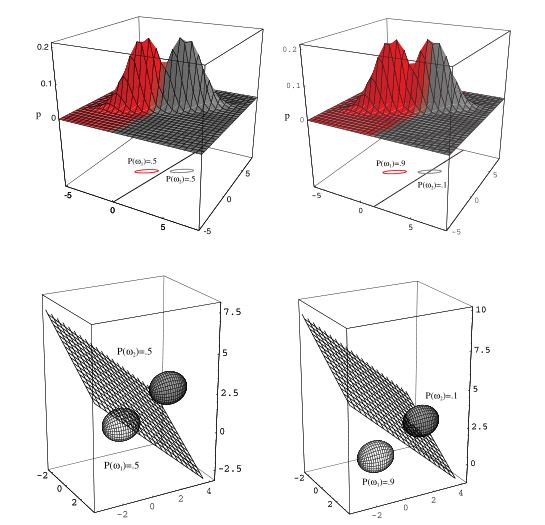
\includegraphics{images/dyskrym2} 

}

\caption{Hiperpłaszczyzna rozdzielająca obszary innych klas może być przesunięta w kierunku bardziej prawdopodobnej klasy, jeśli prawdopodobieństwa a priori są różne. Źródło: @duda2001}\label{fig:hiper2}
\end{figure}

\hypertarget{przypadek-gdy-boldsymbol-sigma_i-jest-dowolnej-postaci}{%
\subsection{\texorpdfstring{Przypadek gdy \(\boldsymbol \Sigma_i\) jest dowolnej postaci}{Przypadek gdy \textbackslash{}boldsymbol \textbackslash{}Sigma\_i jest dowolnej postaci}}\label{przypadek-gdy-boldsymbol-sigma_i-jest-dowolnej-postaci}}

Jest to najbardziej ogólny przypadek, kiedy nie nakłada się żadnych ograniczeń na macierze kowariancji grupowych. Postać funkcji dyskryminacyjnych jest następująca
\begin{equation}
    g_i(\boldsymbol x)=\boldsymbol x'\boldsymbol W_i\boldsymbol x+\boldsymbol w_i'\boldsymbol x+w_{i0}
    \label{eq:row813}
\end{equation}
gdzie
\begin{align}
    \boldsymbol W_i = &-\frac12 \boldsymbol\Sigma_i^{-1},\\
    \boldsymbol w_i=& \boldsymbol\Sigma_i^{-1}\boldsymbol\mu_i,\\
    w_{i0} = &-\frac12\boldsymbol\mu_i'\boldsymbol\Sigma_i^{-1}\boldsymbol\mu_i-\frac12\log|\boldsymbol\Sigma_i|+\log\P(c_i).
\end{align}

Ograniczenia w ten sposób budowane są hiperpowierzchniami (nie koniecznie hiperpłaszczyznami). W literaturze ta metoda znana jest pod nazwą kwadratowej analizy dyskryminacyjnej (ang. \emph{Quadratic Discriminant Analysis}).

\begin{figure}

{\centering 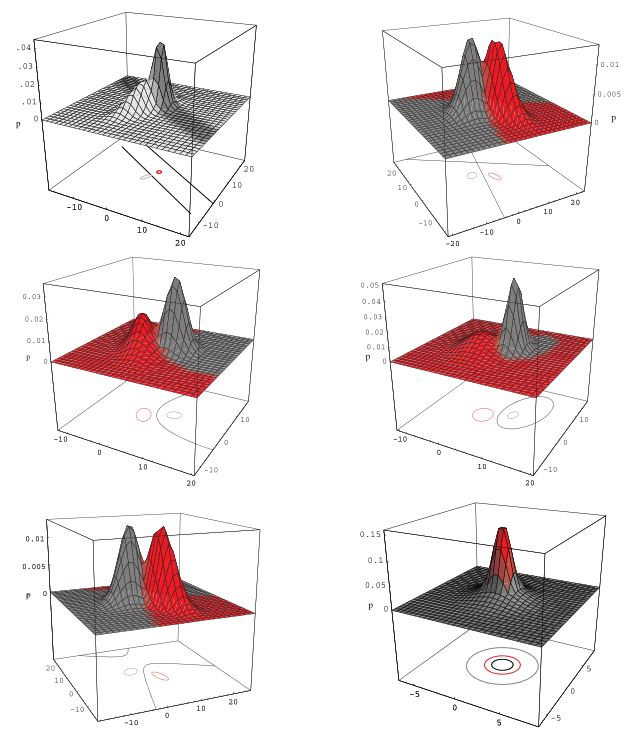
\includegraphics{images/dyskrym3} 

}

\caption{Przykład zastosowania kwadratowej analizy dyskryminacyjnej. Pokazane są dopuszczalne postaci zbiorów ograniczających. Źródło: @duda2001}\label{fig:hiper3}
\end{figure}

\BeginKnitrBlock{example}
\protect\hypertarget{exm:caravan}{}{\label{exm:caravan} }Przeprowadzimy klasyfikację na podstawie zbioru \texttt{Smarket} pakietu \texttt{ILSR}. Dane zawierają kursy indeksu giełdowego S\&P500 w latach 2001-2005. Na podstawie wartości waloru z poprzednich 2 dni będziemy chcieli przewidzieć czy ruch w kolejnym okresie czasu będzie w górę czy w dół.
\EndKnitrBlock{example}

\begin{Shaded}
\begin{Highlighting}[]
\KeywordTok{library}\NormalTok{(ISLR)}
\KeywordTok{head}\NormalTok{(Smarket)}
\end{Highlighting}
\end{Shaded}

\begin{verbatim}
##   Year   Lag1   Lag2   Lag3   Lag4   Lag5 Volume  Today Direction
## 1 2001  0.381 -0.192 -2.624 -1.055  5.010 1.1913  0.959        Up
## 2 2001  0.959  0.381 -0.192 -2.624 -1.055 1.2965  1.032        Up
## 3 2001  1.032  0.959  0.381 -0.192 -2.624 1.4112 -0.623      Down
## 4 2001 -0.623  1.032  0.959  0.381 -0.192 1.2760  0.614        Up
## 5 2001  0.614 -0.623  1.032  0.959  0.381 1.2057  0.213        Up
## 6 2001  0.213  0.614 -0.623  1.032  0.959 1.3491  1.392        Up
\end{verbatim}

\begin{Shaded}
\begin{Highlighting}[]
\KeywordTok{set.seed}\NormalTok{(}\DecValTok{2019}\NormalTok{)}
\NormalTok{dt.ucz <-}\StringTok{ }\NormalTok{Smarket }\OperatorTok\StringTok{ }
\StringTok{    }\KeywordTok{mutate_if}\NormalTok{(is.numeric, scale) }\OperatorTok\StringTok{ }
\StringTok{    }\KeywordTok{sample_frac}\NormalTok{(}\DataTypeTok{size =} \DecValTok{2}\OperatorTok{/}\DecValTok{3}\NormalTok{) }
\NormalTok{dt.test <-}\StringTok{ }\NormalTok{Smarket[}\OperatorTok{-}\KeywordTok{as.numeric}\NormalTok{(}\KeywordTok{rownames}\NormalTok{(dt.ucz)),]}
\NormalTok{mod.qda <-}\StringTok{ }\KeywordTok{qda}\NormalTok{(Direction}\OperatorTok{~}\NormalTok{Lag1}\OperatorTok{+}\NormalTok{Lag2, }\DataTypeTok{data =}\NormalTok{ dt.ucz)}
\NormalTok{mod.qda}
\end{Highlighting}
\end{Shaded}

\begin{verbatim}
## Call:
## qda(Direction ~ Lag1 + Lag2, data = dt.ucz)
## 
## Prior probabilities of groups:
##      Down        Up 
## 0.4789916 0.5210084 
## 
## Group means:
##             Lag1         Lag2
## Down  0.01064899 -0.006153307
## Up   -0.08417078  0.030090639
\end{verbatim}

Ponieważ funkcje dyskryminacyjne mogą być nieliniowe, to podsumowanie modelu nie zawiera współczynników funkcji. Podsumowanie zawiera tylko prawdopodobieństwa a priori i średnie poszczególnych zmiennych niezależnych w klasach.

\begin{Shaded}
\begin{Highlighting}[]
\NormalTok{pred.qda <-}\StringTok{ }\KeywordTok{predict}\NormalTok{(mod.qda, dt.test)}
\NormalTok{tab <-}\StringTok{ }\KeywordTok{table}\NormalTok{(}\DataTypeTok{pred =}\NormalTok{ pred.qda}\OperatorTok{$}\NormalTok{class, dt.test}\OperatorTok{$}\NormalTok{Direction)}
\NormalTok{tab}
\end{Highlighting}
\end{Shaded}

\begin{verbatim}
##       
## pred   Down  Up
##   Down   10  17
##   Up    171 219
\end{verbatim}

\begin{Shaded}
\begin{Highlighting}[]
\KeywordTok{sum}\NormalTok{(}\KeywordTok{diag}\NormalTok{(}\KeywordTok{prop.table}\NormalTok{(tab)))}
\end{Highlighting}
\end{Shaded}

\begin{verbatim}
## [1] 0.5491607
\end{verbatim}

\begin{Shaded}
\begin{Highlighting}[]
\KeywordTok{library}\NormalTok{(klaR)}
\KeywordTok{partimat}\NormalTok{(Direction }\OperatorTok{~}\StringTok{ }\NormalTok{Lag1}\OperatorTok{+}\NormalTok{Lag2, }
         \DataTypeTok{data =}\NormalTok{ dt.ucz,}
         \DataTypeTok{method =} \StringTok{"qda"}\NormalTok{,}
         \DataTypeTok{col.correct=}\StringTok{'blue'}\NormalTok{,}
         \DataTypeTok{col.wrong=}\StringTok{'red'}\NormalTok{)}
\end{Highlighting}
\end{Shaded}

\begin{figure}

{\centering 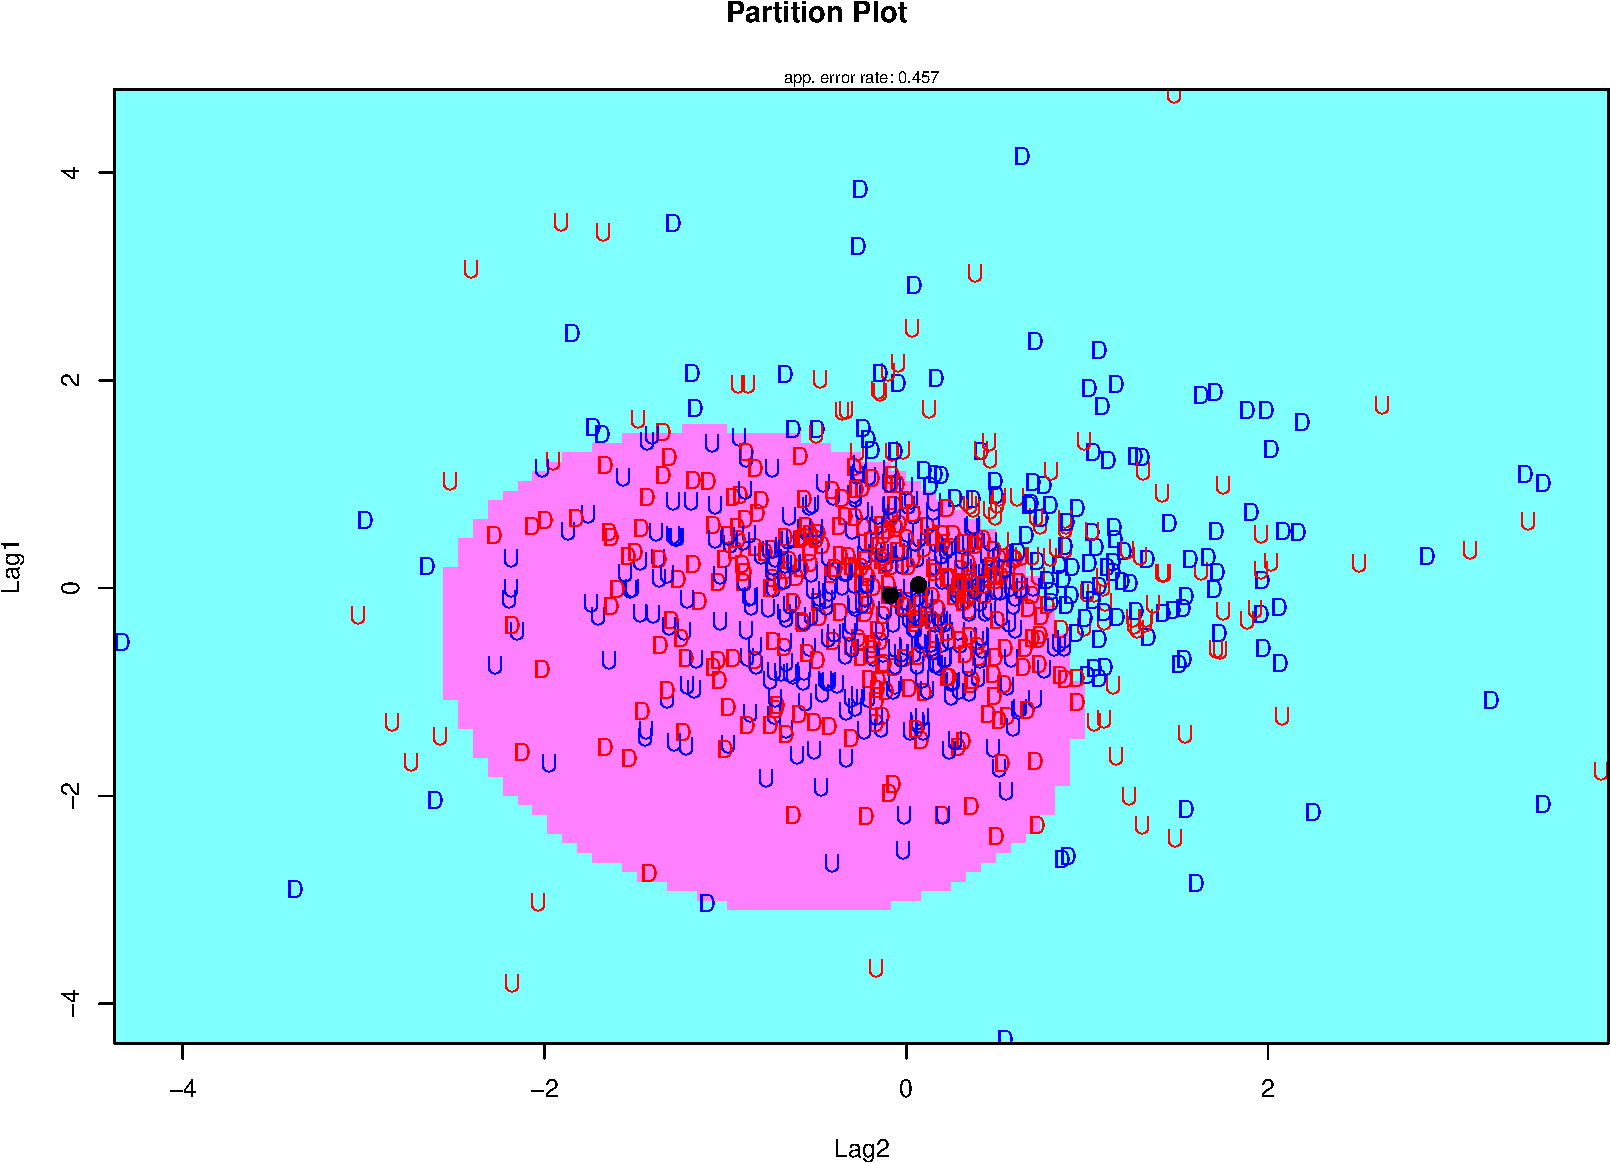
\includegraphics{EksploracjaDanych_files/figure-latex/qda-1} 

}

\caption{Wykres klasyfikacji na podstawie QDA. Obserwacje zaznczone kolorem niebieskim są prawidłowo zaklasyfikowane, a czerwonym źle}\label{fig:qda}
\end{figure}

\hypertarget{analiza-dyskryminacyjna-metoda-czesciowych-najmniejszych-kwadratow}{%
\section{Analiza dyskryminacyjna metodą częściowych najmniejszych kwadratów}\label{analiza-dyskryminacyjna-metoda-czesciowych-najmniejszych-kwadratow}}

Analiza dyskryminacyjna metodą częściowych najmniejszych kwadratów (ang. \emph{Partial Least Squares Discriminant Analysis}) jest wykorzystywana szczególnie w sytuacjach gdy zestaw predyktorów zwiera zmienne silnie ze sobą skorelowane. Jak wiadomo z wcześniejszych rozważań, metody dyskryminacji obserwacji są mało odporne na nadmiarowość zmiennych niezależnych. Stąd powstał pomysł zastosowania połączenia LDA z PLS (Partial Least Squares), której celem jest redukcja wymiaru przestrzeni jednocześnie maksymalizując korelację zmiennych niezależnych ze zmienną wynikową.

Parametrem, który jest kontrolowany podczas budowy modelu jest liczba ukrytych zmiennych. Metoda PLSDA ma kilka implementacji w R, ale najbardziej znana jest funkcja \texttt{plsda} z pakietu \texttt{caret} (Jed Wing et al. \protect\hyperlink{ref-kuhn}{2018}).

\BeginKnitrBlock{example}
\protect\hypertarget{exm:plsda}{}{\label{exm:plsda} }Kontynując poprzedni przykład przeprowadzimy klasyfikacje ruchu waloru korzystając z metody PLSDA. W przeciwieństwie do poprzednich funkcji \texttt{plsda} potrzebuje przekazania zbioru predyktorów i wektora zmiennej wynikowej oddzielnie, a nie za pomocą formuły. Doboru liczby zmiennych latentnych dokonamy arbitralnie.
\EndKnitrBlock{example}

\begin{Shaded}
\begin{Highlighting}[]
\KeywordTok{library}\NormalTok{(caret)}
\NormalTok{mod.plsda <-}\StringTok{ }\KeywordTok{plsda}\NormalTok{(dt.ucz[,}\OperatorTok{-}\KeywordTok{c}\NormalTok{(}\DecValTok{1}\NormalTok{,}\DecValTok{7}\OperatorTok{:}\DecValTok{9}\NormalTok{)],}
                   \KeywordTok{as.factor}\NormalTok{(dt.ucz}\OperatorTok{$}\NormalTok{Direction), }
                   \DataTypeTok{ncomp =} \DecValTok{2}\NormalTok{)}
\NormalTok{mod.plsda}\OperatorTok{$}\NormalTok{loadings}
\end{Highlighting}
\end{Shaded}

\begin{verbatim}
## 
## Loadings:
##      Comp 1 Comp 2
## Lag1 -0.712  0.450
## Lag2  0.234  0.237
## Lag3  0.647       
## Lag4  0.158  0.519
## Lag5         0.681
## 
##                Comp 1 Comp 2
## SS loadings     1.008  1.001
## Proportion Var  0.202  0.200
## Cumulative Var  0.202  0.402
\end{verbatim}

Dwie ukryte zmienne użyte do redukcji wymiaru przestrzeni wyjaśniają około 40\% zmienności pierwotnych zmiennych. Ładunki (\texttt{Loadings}) pokazują kontrybucje poszczególnych zmiennych w tworzenie się zmiennych ukrytych.

\begin{Shaded}
\begin{Highlighting}[]
\NormalTok{pred.plsda <-}\StringTok{ }\KeywordTok{predict}\NormalTok{(mod.plsda, dt.test[,}\OperatorTok{-}\KeywordTok{c}\NormalTok{(}\DecValTok{1}\NormalTok{,}\DecValTok{7}\OperatorTok{:}\DecValTok{9}\NormalTok{)])}
\NormalTok{tab <-}\StringTok{ }\KeywordTok{table}\NormalTok{(pred.plsda, dt.test}\OperatorTok{$}\NormalTok{Direction)}
\NormalTok{tab}
\end{Highlighting}
\end{Shaded}

\begin{verbatim}
##           
## pred.plsda Down  Up
##       Down   37  50
##       Up    144 186
\end{verbatim}

\begin{Shaded}
\begin{Highlighting}[]
\KeywordTok{sum}\NormalTok{(}\KeywordTok{diag}\NormalTok{(}\KeywordTok{prop.table}\NormalTok{(tab)))}
\end{Highlighting}
\end{Shaded}

\begin{verbatim}
## [1] 0.5347722
\end{verbatim}

Ponieważ korelacje pomiędzy predyktorami w naszym przypadku nie były duże, to zastosowanie PLSDA nie poprawiło znacząco klasyfikacji w stosunku do metody QDA.

\begin{Shaded}
\begin{Highlighting}[]
\KeywordTok{cor}\NormalTok{(dt.ucz[,}\DecValTok{2}\OperatorTok{:}\DecValTok{6}\NormalTok{])}
\end{Highlighting}
\end{Shaded}

\begin{verbatim}
##              Lag1         Lag2         Lag3        Lag4        Lag5
## Lag1  1.000000000 -0.001713222  0.003820374  0.01583203  0.02504524
## Lag2 -0.001713222  1.000000000 -0.046611448 -0.02069792 -0.04105822
## Lag3  0.003820374 -0.046611448  1.000000000 -0.06142632 -0.03424691
## Lag4  0.015832026 -0.020697920 -0.061426325  1.00000000 -0.07102928
## Lag5  0.025045238 -0.041058218 -0.034246907 -0.07102928  1.00000000
\end{verbatim}

\hypertarget{regularyzowana-analiza-dyskryminacyjna}{%
\section{Regularyzowana analiza dyskryminacyjna}\label{regularyzowana-analiza-dyskryminacyjna}}

Regularyzowana analiza dyskryminacyjna (ang. \emph{Regularized Discriminant Analysis}) powstała jako technika równoważąca zalety i wady LDA i QDA. Ze względu na zdolności generalizacyjne model LDA jest lepszy od QDA (mniejsza wariancja modelu), ale jednocześnie QDA ma bardziej elastyczną postać hiperpowierzchni brzegowych rozdzielających obiekty różnych klas. Dlatego Friedman (\protect\hyperlink{ref-friedman1989}{1989}) wprowadził technikę będącą kompromisem pomiędzy LDA i QDA poprzez odpowiednie określenie macierzy kowariancji
\begin{equation}
    \tilde{\boldsymbol \Sigma}_i(\lambda) = \lambda\boldsymbol\Sigma_i + (1-\lambda)\boldsymbol\Sigma,
\end{equation}
gdzie \(\boldsymbol \Sigma_i\) jest macierzą kowariancji dla \(i\)-tej klasy, a \(\boldsymbol \Sigma\) jest uśrednioną macierzą kowariancji wszystkich klas. Zatem odpowiedni dobór parametru \(\lambda\) decyduje czy poszukujemy modelu prostszego (\(\lambda = 0\) odpowiada LDA), czy bardziej elastycznego (\(\lambda=1\) oznacza QDA).

Dodatkowo metoda RDA pozwala na elastyczny wybór pomiędzy postaciami macierzy kowariancji wspólnej dla wszystkich klas \(\boldsymbol\Sigma\). Może ona być macierzą jednostkową, jak w przypadku \ref{przypI}, co oznacza niezależność predyktorów modelu, może też być jak w przypadku \ref{przypSig}, gdzie dopuszcza się korelacje między predyktorami. Dokonuje się tego przez odpowiedni dobór parametru \(\gamma\)
\begin{equation}
    \boldsymbol \Sigma(\gamma) = \gamma\boldsymbol \Sigma+(1-\gamma)\sigma^2I.
\end{equation}

\BeginKnitrBlock{example}
\protect\hypertarget{exm:rda}{}{\label{exm:rda} }Funkcja \texttt{rda} pakietu \texttt{klaR} jest implementacją powyższej metody. Ilustrają jej działania będzie klasyfikacja stanów z poprzedniego przykładu.
\EndKnitrBlock{example}

\begin{Shaded}
\begin{Highlighting}[]
\KeywordTok{library}\NormalTok{(klaR)}
\NormalTok{mod.rda <-}\StringTok{ }\KeywordTok{rda}\NormalTok{(Direction}\OperatorTok{~}\NormalTok{Lag1}\OperatorTok{+}\NormalTok{Lag2}\OperatorTok{+}\NormalTok{Lag3}\OperatorTok{+}\NormalTok{Lag4}\OperatorTok{+}\NormalTok{Lag5, dt.ucz)}
\NormalTok{mod.rda}
\end{Highlighting}
\end{Shaded}

\begin{verbatim}
## Call: 
## rda(formula = Direction ~ Lag1 + Lag2 + Lag3 + Lag4 + Lag5, data = dt.ucz)
## 
## Regularization parameters: 
##      gamma     lambda 
## 0.33416870 0.03931045 
## 
## Prior probabilities of groups: 
##      Down        Up 
## 0.4789916 0.5210084 
## 
## Misclassification rate: 
##        apparent: 43.337 %
## cross-validated: 45.524 %
\end{verbatim}

Model został oszacowany z parametrami wyznaczonymi na podstawie sprawdzianu krzyżowego zastosowanego w funkcji \texttt{rda}.

\begin{Shaded}
\begin{Highlighting}[]
\NormalTok{pred.rda <-}\StringTok{ }\KeywordTok{predict}\NormalTok{(mod.rda, dt.test)}
\NormalTok{(tab <-}\StringTok{ }\KeywordTok{table}\NormalTok{(}\DataTypeTok{pred =}\NormalTok{ pred.rda}\OperatorTok{$}\NormalTok{class, dt.test}\OperatorTok{$}\NormalTok{Direction))}
\end{Highlighting}
\end{Shaded}

\begin{verbatim}
##       
## pred   Down  Up
##   Down   19  30
##   Up    162 206
\end{verbatim}

\begin{Shaded}
\begin{Highlighting}[]
\KeywordTok{sum}\NormalTok{(}\KeywordTok{diag}\NormalTok{(}\KeywordTok{prop.table}\NormalTok{(tab)))}
\end{Highlighting}
\end{Shaded}

\begin{verbatim}
## [1] 0.5395683
\end{verbatim}

Jakość klasyfikacji jest na zbliżonym poziomie jak przy poprzednich metodach.

\hypertarget{analiza-dyskryminacyjna-mieszana}{%
\section{Analiza dyskryminacyjna mieszana}\label{analiza-dyskryminacyjna-mieszana}}

Liniowa analiza dyskryminacyjna zakładała, że średnie (centroidy) w klasach są różne ale macierz kowariancji wszystkich klas jest jednakowa. Analiza dyskryminacyjna mieszana (ang. \emph{Mixture Discriminant Analysis}) prezentuje jeszcze inne podejście ponieważ zakłada, że każda klasa może być charakteryzowana przez wiele wielowymiarowych rozkładów normalnych, których centroidy mogą się różnic, ale macierze kowariancji nie.

Wówczas rozkład dla danej klasy jest mieszaniną rozkładów składowych, a funkcja dyskryminacyjna dla \(i\)-tej klasy przyjmuje postać
\begin{equation}
    g_i(\boldsymbol x)\propto \sum_{k=1}^{L_i}\phi_{ik}g_{ik}(\boldsymbol x),
\end{equation}
gdzie \(L_i\) jest liczbą rozkładów składających się na \(i\)-tą klasę, a \(\phi_{ik}\) jest współczynnikiem proporcji estymowanych w czasie uczenia modelu.

\BeginKnitrBlock{example}
\protect\hypertarget{exm:mda}{}{\label{exm:mda} }Funkcja \texttt{mda} pakietu \texttt{mda} (Trevor Hastie et al. \protect\hyperlink{ref-R-mda}{2017}) jest implementacją tej techniki w R. Jej zastosowanie pokażemy na przykładzie danych giełdowych z poprzedniego przykładu. Użyjemy domyślnych ustawień funkcji (trzy rozkłady dla każdej klasy).
\EndKnitrBlock{example}

\begin{Shaded}
\begin{Highlighting}[]
\KeywordTok{library}\NormalTok{(mda)}
\NormalTok{mod.mda <-}\StringTok{ }\KeywordTok{mda}\NormalTok{(Direction}\OperatorTok{~}\NormalTok{Lag1}\OperatorTok{+}\NormalTok{Lag2}\OperatorTok{+}\NormalTok{Lag3}\OperatorTok{+}\NormalTok{Lag4}\OperatorTok{+}\NormalTok{Lag5, dt.ucz)}
\NormalTok{mod.mda}
\end{Highlighting}
\end{Shaded}

\begin{verbatim}
## Call:
## mda(formula = Direction ~ Lag1 + Lag2 + Lag3 + Lag4 + Lag5, data = dt.ucz)
## 
## Dimension: 5 
## 
## Percent Between-Group Variance Explained:
##     v1     v2     v3     v4     v5 
##  48.45  88.33  94.80  99.68 100.00 
## 
## Degrees of Freedom (per dimension): 6 
## 
## Training Misclassification Error: 0.42737 ( N = 833 )
## 
## Deviance: 1134.453
\end{verbatim}

\begin{Shaded}
\begin{Highlighting}[]
\NormalTok{pred.mda <-}\StringTok{ }\KeywordTok{predict}\NormalTok{(mod.mda, dt.test)}
\NormalTok{(tab <-}\StringTok{ }\KeywordTok{table}\NormalTok{(}\DataTypeTok{pred =}\NormalTok{ pred.mda, dt.test}\OperatorTok{$}\NormalTok{Direction))}
\end{Highlighting}
\end{Shaded}

\begin{verbatim}
##       
## pred   Down  Up
##   Down   23  38
##   Up    158 198
\end{verbatim}

\begin{Shaded}
\begin{Highlighting}[]
\KeywordTok{sum}\NormalTok{(}\KeywordTok{diag}\NormalTok{(}\KeywordTok{prop.table}\NormalTok{(tab)))}
\end{Highlighting}
\end{Shaded}

\begin{verbatim}
## [1] 0.529976
\end{verbatim}

Kolejny raz model dyskryminacyjny charakteryzuje się podobną jakością klasyfikacji.

\hypertarget{elastyczna-analiza-dyskryminacyjna}{%
\section{Elastyczna analiza dyskryminacyjna}\label{elastyczna-analiza-dyskryminacyjna}}

Zupełnie inne podejście w stosunku do wcześniejszych rozwiązań, prezentuje elastyczna analiza dyskryminacyjna (ang. \emph{Flexible Discriminant Analysis}) . Kodując klasy wynikowe jako zmienne dychotomiczne (dla każdej klasy jest odrębna zmienna wynikowa) dla każdej z nich budowanych jest \(k\) modeli regresji. Mogą to być modele regresji penalizowanej, jak regresja grzbietowa lub LASSO, modele regresji wielomianowej albo modele regresji sklejanej (MARS), o których będzie mowa w dalszej części tego opracowania.

Przykładowo, jeśli modelem bazowym jest MARS, to funkcja dyskryminacyjna \(i\)-tej klasy może być postaci
\begin{equation}
    g_i(\boldsymbol x)=\beta_0+\beta_1h(1-x_1)+\beta_2h(x_2-1)+\beta_3h(1-x_3)+\beta_4h(x_1-1),
\end{equation}
gdzie \(h\) są tzw. funkcjami bazowymi postaci
\begin{equation}
    h(x)= \begin{cases}
        x, & x> 0\\
        0, & x\leq 0.
    \end{cases}
\end{equation}
Klasyfikacji dokonujemy sprawdzając znak funkcji dyskryminacyjnej \(g_i\), jeśli jest dodatni, to funkcja przypisuje obiekt do klasy \(i\)-tej. W przeciwnym przypadku nie należy do tej klasy.

\begin{figure}

{\centering 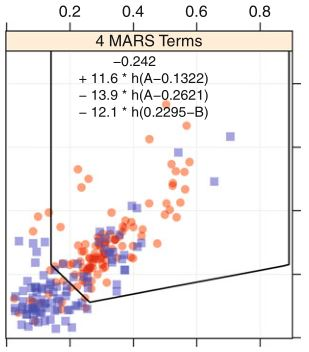
\includegraphics{images/fda} 

}

\caption{Przykład klasyfikacji dwustanowej za pomocą metody FDA}\label{fig:fda}
\end{figure}

\BeginKnitrBlock{example}
\protect\hypertarget{exm:przykFDA}{}{\label{exm:przykFDA} }Funkcja \texttt{fda} pakietu \texttt{mda} jest implementacją techniki FDA w R. Na postawie danych z poprzedniego przykładu zostanie przedstawiona zasada dziełania. Przyjmiemy domyślne ustawienia funkcji, z wyjątkiem metody estymacji modelu, jako którą przyjmiemy MARS.
\EndKnitrBlock{example}

\begin{Shaded}
\begin{Highlighting}[]
\NormalTok{mod.fda <-}\StringTok{ }\KeywordTok{fda}\NormalTok{(Direction}\OperatorTok{~}\NormalTok{Lag1}\OperatorTok{+}\NormalTok{Lag2, dt.ucz, }\DataTypeTok{method =}\NormalTok{ mars)}
\NormalTok{mod.fda}
\end{Highlighting}
\end{Shaded}

\begin{verbatim}
## Call:
## fda(formula = Direction ~ Lag1 + Lag2, data = dt.ucz, method = mars)
## 
## Dimension: 1 
## 
## Percent Between-Group Variance Explained:
##  v1 
## 100 
## 
## Training Misclassification Error: 0.43938 ( N = 833 )
\end{verbatim}

Ponieważ, zmienna wynikowa jest dwustanowa, to powstała tylko jedna funkcja dyskryminacyjna.
Parametry modelu są następujące

\begin{Shaded}
\begin{Highlighting}[]
\NormalTok{mod.fda}\OperatorTok{$}\NormalTok{fit}\OperatorTok{$}\NormalTok{coefficients}
\end{Highlighting}
\end{Shaded}

\begin{verbatim}
##            [,1]
## [1,]  0.1129623
## [2,] -0.5202437
## [3,]  0.5462219
\end{verbatim}

\begin{Shaded}
\begin{Highlighting}[]
\NormalTok{pred.fda <-}\StringTok{ }\KeywordTok{predict}\NormalTok{(mod.fda, dt.test)}
\NormalTok{(tab <-}\StringTok{ }\KeywordTok{table}\NormalTok{(}\DataTypeTok{pred =}\NormalTok{ pred.fda, dt.test}\OperatorTok{$}\NormalTok{Direction))}
\end{Highlighting}
\end{Shaded}

\begin{verbatim}
##       
## pred   Down  Up
##   Down  108 118
##   Up     73 118
\end{verbatim}

\begin{Shaded}
\begin{Highlighting}[]
\KeywordTok{sum}\NormalTok{(}\KeywordTok{diag}\NormalTok{(}\KeywordTok{prop.table}\NormalTok{(tab)))}
\end{Highlighting}
\end{Shaded}

\begin{verbatim}
## [1] 0.5419664
\end{verbatim}

Jakość klasyfikacji jest tylko nieco lepsza niż w przypadku poprzednich metod.

\hypertarget{bayes}{%
\chapter{Klasyfikatory bayesowskie}\label{bayes}}

Całą gamę klasyfikatorów opartych na twierdzeniu Bayesa nazywać będziemy bayesowskimi.
\begin{equation}\label{bayes}
        P(A|B)=\frac{P(A)P(B|A)}{P(B)},
\end{equation}
gdzie \(P(B)>0\).

Bayesowskie reguły podejmowania decyzji dały podstawy takich metod jak:

\begin{itemize}
\tightlist
\item
  liniowa analiza dyskryminacyjna;
\item
  kwadratowa analiza dyskryminacyjna;
\end{itemize}

W ustaleniu klasyfikatora bayesowskiego będzie nam przyświecała cały czas ta sama reguła: \emph{jeśli znam wartości cech charakteryzujących badane obiekty oraz klasy do których należą (w próbie uczącej), to na ich podstawie mogę wyznaczyć miary prawdopodobieństw a posteriori, które pomogą mi w ustaleniu klasy do której należy nowy testowy element.}

W dalszej części będziemy przyjmowali następujące oznaczenia:

\begin{itemize}
\tightlist
\item
  \(T\) - zbiór danych uczących (treningowych),
\item
  \(T^j\) - zbiór danych uczących dla których przyjęliśmy decyzję o przynależności do \(j\)-tej klasy,
\item
  \(T^j_{a_i=v}\) - zbiór danych uczących o wartości atrybutu \(a_i\) równej \(v\) i klasy \(j\)-tej,
\item
  \(\mathbb{H}\) - przestrzeń hipotez,
\item
  \(P(h|a_1=v_1, a_2=v_2,\ldots,a_p=v_p)\) - prawdopodobieństwo a posteriori, że prawdziwa jest hipoteza \(h\in \mathbb{H}\), jeśli znamy atrybuty obiektu,
\item
  \(P(h)\) - prawdopodobieństwo a priori zajścia hipotezy \(h\in \mathbb{H}\),
\item
  \(c\) - prawdziwy stan obiektu.
\end{itemize}

\hypertarget{klasyfikator-maximum-a-posteriori-map}{%
\section{Klasyfikator maximum a posteriori (MAP)}\label{klasyfikator-maximum-a-posteriori-map}}

Na podstawie wiedzy o atrybutach obiektu \(x\) podejmujemy decyzję o klasyfikacji tego obiektu zgodnie z hipotezą \(h_{MAP}\in \mathbb{H}\), która przyjmuje postać
\begin{align}\label{MAP}
        h_{MAP}=&\operatorname{arg}\max_{h\in \mathbb{H}}P(h|a_1=v_1, a_2=v_2,\ldots,a_p=v_p)\\
            =& \operatorname{arg}\max_{h\in \mathbb{H}}P(a_1=v_1, a_2=v_2,\ldots,a_p=v_p|h)\cdot P(h),
\end{align}
gdzie ostatnia równość wynika z twierdzenia Bayesa oraz faktu, że dla konkretnego obiektu \(x\) wielkości atrybutów nie zależą od postawionej hipotezy.

\hypertarget{klasyfikator-najwiekszej-wiarogodnosci-ml}{%
\section{Klasyfikator największej wiarogodności (ML)}\label{klasyfikator-najwiekszej-wiarogodnosci-ml}}

Na podstawie wiedzy o atrybutach obiektu \(x\) podejmujemy decyzję o klasyfikacji tego obiektu zgodnie z hipotezą \(h_{ML}\in \mathbb{H}\), która przyjmuje postać
\begin{equation}\label{ML}
        h_{ML}=\operatorname{arg}\max_{h\in \mathbb{H}}P(a_1=v_1, a_2=v_2,\ldots,a_p=v_p|h).
\end{equation}

\BeginKnitrBlock{remark}
\iffalse{} {Uwaga. } \fi{}Obie wspomniane metody wymagają znajomości prawdopodobieństwa \(P(a_1=v_1,a_2=v_2,\ldots,a_p=v_p|h)\), ale różnią się podejściem do wiedzy o prawdopodobieństwach a priori. W metodzie MAP brana pod uwagę jest wiedza o prawdopodobieństwie przynależności do poszczególnych klas, a w ML nie. Dla klasyfikacji, w których prawdopodobieństwa przynależności do klas są takie same, klasyfikatory MAP i ML są równoważne.
\EndKnitrBlock{remark}

\hypertarget{naiwny-klasyfikator-bayesa-nb}{%
\section[Naiwny klasyfikator Bayesa (NB)]{\texorpdfstring{Naiwny klasyfikator Bayesa (NB)\footnote{ang. \emph{Naive Bayes Classifier}}}{Naiwny klasyfikator Bayesa (NB)}}\label{naiwny-klasyfikator-bayesa-nb}}

Największy problem w wyznaczeniu klasyfikatorów MAP i ML stanowi wyznaczenie rozkładu łącznego \(P(a_1=v_1, a_2=v_2,\ldots,a_p=v_p|h)\). W naiwnym klasyfikatorze Bayesa zakłada się niezależność warunkową poszczególnych atrybutów względem klasy do której ma należeń wg hipotezy obiekt. Założenie to często nie jest spełnione i stąd nazwa przymiotnik ``naiwny''.

Definicja naiwnego klasyfikatora bayesowskiego różni się od klasyfikatora MAP tylko podejściem do prawdopodobieństwa a posteriori.
\begin{equation}\label{naiwny_bayes}
        h_{NB}=\operatorname{arg}\max_{h_j\in \mathbb{H}}P(h_j)\prod_{i=1}^{p}P(a_i=v_i|h_j),
\end{equation}
gdzie \(h_j\) oznacza hipotezę (decyzję), że badany obiekt należy do \(j\)-tej klasy.

Oczywiście zarówno prawdopodobieństwo a priori jak i a posteriori są wyznaczane na podstawie próby, i tak prawdopodobieństwo a priori wynosi
\begin{equation}\label{apriori}
        P(h_j)=P_T(h_j)=\frac{|T^j|}{|T|}, 
\end{equation}
gdzie \(|A|\) oznacza moc zbioru \(A\).

Natomiast prawdopodobieństwo a posteriori dla \(i\)-tego atrybutu wynosi
\begin{equation}\label{aposteriori}
        P(a_i=v_i|h_j)=P_{T^j}(a_i=v_i)=\frac{|T^j_{a_i=v_i}|}{|T^j|}.
\end{equation}
Na mocy powyższego możemy zauważyć, że jeżeli założenie o warunkowej niezależności jest spełnione, to klasyfikatory NB i MAP są równoważne.

Chcąc przypisać klasę nowemu obiektowi powstaje problem praktyczny, polegający na tym, że dla pewnych konfiguracji atrybutów nie ma odpowiedników w nauczonym modelu. Powodem takiego stanu rzeczy jest fakt, że takie kombinacje nie wystąpiły w próbie uczącej.

Istnieją dwa sposoby predykcji w takiej sytuacji:

\begin{enumerate}
\def\labelenumi{\arabic{enumi}.}
\tightlist
\item
  \begin{equation}\label{pred1}
           P(a_i=v_i|h_j)=
           \begin{cases}
               \frac{|T^j_{a_i=v_i}|}{|T^j|}, & T^j_{a_i=v_i}\neq \emptyset\\
               \epsilon, & \text{w przeciwnym przypadku.}
           \end{cases}
   \end{equation}
  W tym przypadku przyjmuje się, że \(\epsilon \ll 1/|T_j|\).
\item
  Drugi sposób wykorzystuje estymację z poprawką
  \begin{equation}\label{pred2}
       P(a_i=v_i|h_j)=\frac{|T^j_{a_i=v_i}|+mp}{|T^j|+mp},
  \end{equation}
  gdzie \(p\) oznacza prawdopodobieństwo a priori przyjęcia przez atrybut \(a\) wartości \(v\) (najczęściej \(p=1/|A|\), \(A\) - zbiór wszystkich możliwych wartości atrybutu \(a\)), \(m\) - waga (najczęściej \(m=|A|\)).
\end{enumerate}

W przypadku gdy atrybuty są mierzone na skali ciągłej najczęściej stosuje się dyskretyzację ich do zmiennych ze skali przedziałowej. Inna metoda stosowana w przypadku ciągłych atrybutów, to użycie gęstości \(g_i^j\) o rozkładzie normalnym w miejsce \(P(a_i=v_i|h_j)\). Przy czym do obliczenia parametrów rozkładu stosujemy wzory
\begin{equation}\label{sred}
        m_i^j=\frac{1}{|T^j|}\sum_{x\in T^j}a_i(x),
\end{equation}
oraz
\begin{equation}\label{odch}
        (s_i^j)^2=\frac{1}{|T^j|-1}\sum_{x\in T^j}(a_i(x)-m_i^j)^2.
\end{equation}

Obsługa braków danych przez naiwny klasyfikator Bayesa jest dość prosta i opiera się na liczeniu prawdopodobieństw a posteriori wyłącznie dla obiektów, których wartości atrybutów są znane. Dlatego prawdopodobieństwa warunkowe liczy się wg wzoru
\begin{equation}\label{pr_war}
        P(a_i=v_i|h_j)=\frac{|T^j_{a_i=v_i}|}{|T^j|-|T^j_{a_i=NA}|}.
\end{equation}
Jeśli brakujące dane nie niosą w sobie istotnych informacji dotyczących klasyfikacji obiektów, to naiwny klasyfikator Bayesa będzie działał poprawnie.

Naiwny klasyfikator Bayesa jest implementowany w pakietach \textbf{e1071} (Meyer et al. \protect\hyperlink{ref-R-e1071}{2019}) i \textbf{klaR} (Weihs et al. \protect\hyperlink{ref-R-klaR}{2005}).

\BeginKnitrBlock{example}
\protect\hypertarget{exm:unnamed-chunk-74}{}{\label{exm:unnamed-chunk-74} }Przeprowadzimy klasyfikację dla zbioru \texttt{Titanic}. W przypadku funkcji z pakietu \texttt{e1071} nie potrzeba zamieniać tabeli na przypadki. W pakiecie \texttt{klaR} istnieje inna funkcja budująca klasyfikator Bayesa \texttt{NaiveBayes}, ale w tym przypadku jeśli zbiór jest w formie tabeli, to należy go zamienić na ramkę danych z oddzielnymi przypadkami.
\EndKnitrBlock{example}

\begin{Shaded}
\begin{Highlighting}[]
\KeywordTok{library}\NormalTok{(e1071)}
\NormalTok{Titanic}
\end{Highlighting}
\end{Shaded}

\begin{verbatim}
## , , Age = Child, Survived = No
## 
##       Sex
## Class  Male Female
##   1st     0      0
##   2nd     0      0
##   3rd    35     17
##   Crew    0      0
## 
## , , Age = Adult, Survived = No
## 
##       Sex
## Class  Male Female
##   1st   118      4
##   2nd   154     13
##   3rd   387     89
##   Crew  670      3
## 
## , , Age = Child, Survived = Yes
## 
##       Sex
## Class  Male Female
##   1st     5      1
##   2nd    11     13
##   3rd    13     14
##   Crew    0      0
## 
## , , Age = Adult, Survived = Yes
## 
##       Sex
## Class  Male Female
##   1st    57    140
##   2nd    14     80
##   3rd    75     76
##   Crew  192     20
\end{verbatim}

\begin{Shaded}
\begin{Highlighting}[]
\NormalTok{nb <-}\StringTok{ }\KeywordTok{naiveBayes}\NormalTok{(Survived }\OperatorTok{~}\StringTok{ }\NormalTok{., }\DataTypeTok{data =}\NormalTok{ Titanic)}
\NormalTok{nb}\OperatorTok{$}\NormalTok{apriori}
\end{Highlighting}
\end{Shaded}

\begin{verbatim}
## Survived
##   No  Yes 
## 1490  711
\end{verbatim}

Poniższe tabele zawierają warunkowe prawdopodobieństwa przynależności do poszczególnych klas.

\begin{Shaded}
\begin{Highlighting}[]
\NormalTok{nb}\OperatorTok{$}\NormalTok{tables}
\end{Highlighting}
\end{Shaded}

\begin{verbatim}
## $Class
##         Class
## Survived        1st        2nd        3rd       Crew
##      No  0.08187919 0.11208054 0.35436242 0.45167785
##      Yes 0.28551336 0.16596343 0.25035162 0.29817159
## 
## $Sex
##         Sex
## Survived       Male     Female
##      No  0.91543624 0.08456376
##      Yes 0.51617440 0.48382560
## 
## $Age
##         Age
## Survived      Child      Adult
##      No  0.03489933 0.96510067
##      Yes 0.08016878 0.91983122
\end{verbatim}

\begin{Shaded}
\begin{Highlighting}[]
\NormalTok{dane <-}\StringTok{ }\KeywordTok{as.data.frame}\NormalTok{(Titanic)}
\NormalTok{pred <-}\StringTok{ }\KeywordTok{predict}\NormalTok{(nb, dane)}
\NormalTok{pred}
\end{Highlighting}
\end{Shaded}

\begin{verbatim}
##  [1] Yes No  No  No  Yes Yes Yes Yes No  No  No  No  Yes Yes Yes Yes Yes
## [18] No  No  No  Yes Yes Yes Yes No  No  No  No  Yes Yes Yes Yes
## Levels: No Yes
\end{verbatim}

\begin{Shaded}
\begin{Highlighting}[]
\NormalTok{tab <-}\StringTok{ }\KeywordTok{table}\NormalTok{(pred, dane}\OperatorTok{$}\NormalTok{Survived)}
\NormalTok{tab}
\end{Highlighting}
\end{Shaded}

\begin{verbatim}
##      
## pred  No Yes
##   No   7   7
##   Yes  9   9
\end{verbatim}

\begin{Shaded}
\begin{Highlighting}[]
\KeywordTok{sum}\NormalTok{(}\KeywordTok{diag}\NormalTok{(}\KeywordTok{prop.table}\NormalTok{(tab)))}
\end{Highlighting}
\end{Shaded}

\begin{verbatim}
## [1] 0.5
\end{verbatim}

Naiwny klasyfikator spisał się bardzo słabo, ponieważ klasyfikacja na poziomie 0.5 jest taka jak przy rzucie monetą.

\BeginKnitrBlock{example}
\protect\hypertarget{exm:unnamed-chunk-78}{}{\label{exm:unnamed-chunk-78} }Przeprowadzimy klasyfikację gatunków irysów na podstawie szerokości i długości kielicha i płatka.
\EndKnitrBlock{example}

\begin{Shaded}
\begin{Highlighting}[]
\KeywordTok{library}\NormalTok{(klaR)}
\KeywordTok{set.seed}\NormalTok{(}\DecValTok{2019}\NormalTok{)}
\NormalTok{uczaca <-}\StringTok{ }\KeywordTok{sample}\NormalTok{(}\DecValTok{1}\OperatorTok{:}\KeywordTok{nrow}\NormalTok{(iris), }\DecValTok{2}\OperatorTok{*}\KeywordTok{nrow}\NormalTok{(iris)}\OperatorTok{/}\DecValTok{3}\NormalTok{)}
\NormalTok{pr.ucz <-}\StringTok{ }\NormalTok{iris[uczaca,]}
\NormalTok{pr.test <-}\StringTok{ }\NormalTok{iris[}\OperatorTok{-}\NormalTok{uczaca,]}
\NormalTok{nb2 <-}\StringTok{ }\KeywordTok{NaiveBayes}\NormalTok{(Species}\OperatorTok{~}\NormalTok{., }\DataTypeTok{data =}\NormalTok{ pr.ucz)}
\NormalTok{nb2}\OperatorTok{$}\NormalTok{apriori}
\end{Highlighting}
\end{Shaded}

\begin{verbatim}
## grouping
##     setosa versicolor  virginica 
##       0.36       0.31       0.33
\end{verbatim}

Prawdopodobieństwa a priori zostały oszacowane na podstawie próby uczącej. Poniższe tabele zawierają średnie i odchylenia standardowe zmiennych w poszczególnych klasach.

\begin{Shaded}
\begin{Highlighting}[]
\NormalTok{nb2}\OperatorTok{$}\NormalTok{tables}
\end{Highlighting}
\end{Shaded}

\begin{verbatim}
## $Sepal.Length
##                [,1]      [,2]
## setosa     4.994444 0.3438807
## versicolor 5.977419 0.5613731
## virginica  6.603030 0.7359029
## 
## $Sepal.Width
##                [,1]      [,2]
## setosa     3.436111 0.3586903
## versicolor 2.838710 0.2996414
## virginica  2.942424 0.3211603
## 
## $Petal.Length
##                [,1]      [,2]
## setosa     1.472222 0.1782632
## versicolor 4.316129 0.4576001
## virginica  5.606061 0.6269666
## 
## $Petal.Width
##                 [,1]       [,2]
## setosa     0.2444444 0.09394358
## versicolor 1.3354839 0.18537959
## virginica  2.0000000 0.25860201
\end{verbatim}

\begin{Shaded}
\begin{Highlighting}[]
\NormalTok{pred <-}\StringTok{ }\KeywordTok{predict}\NormalTok{(nb2, }\DataTypeTok{newdata =}\NormalTok{ pr.test)}
\NormalTok{tab <-}\StringTok{ }\KeywordTok{table}\NormalTok{(pred}\OperatorTok{$}\NormalTok{class, pr.test}\OperatorTok{$}\NormalTok{Species)}
\NormalTok{tab}
\end{Highlighting}
\end{Shaded}

\begin{verbatim}
##             
##              setosa versicolor virginica
##   setosa         14          0         0
##   versicolor      0         18         1
##   virginica       0          1        16
\end{verbatim}

\begin{Shaded}
\begin{Highlighting}[]
\KeywordTok{sum}\NormalTok{(}\KeywordTok{diag}\NormalTok{(}\KeywordTok{prop.table}\NormalTok{(tab)))}
\end{Highlighting}
\end{Shaded}

\begin{verbatim}
## [1] 0.96
\end{verbatim}

Klasyfikacja na podstawie modelu jest bardzo dobra (96\%).

\hypertarget{zalety-i-wady-1}{%
\section{Zalety i wady}\label{zalety-i-wady-1}}

\begin{itemize}
\tightlist
\item
  Zalety:

  \begin{itemize}
  \tightlist
  \item
    prostota konstrukcji i prosty algorytm;
  \item
    jeśli jest spełnione założenie warunkowej niezależności, to ten klasyfikator działa szybciej i czasem lepiej niż inne metody klasyfikacji;
  \item
    nie potrzebuje dużych zbiorów danych do estymacji parametrów;
  \end{itemize}
\item
  Wady:

  \begin{itemize}
  \tightlist
  \item
    często nie spełnione założenie o warunkowej niezależności powoduje obciążenie wyników;
  \item
    brak możliwości wprowadzania interakcji efektów kilku zmiennych;
  \item
    potrzebuje założenia normalności warunkowych gęstości w przypadku ciągłych atrybutów;
  \item
    często istnieją lepsze klasyfikatory.
  \end{itemize}
\end{itemize}

\hypertarget{metoda-k-najblizszych-sasiadow}{%
\chapter{\texorpdfstring{Metoda \(k\) najbliższych sąsiadów}{Metoda k najbliższych sąsiadów}}\label{metoda-k-najblizszych-sasiadow}}

Technika \(k\) najbliższych sąsiadów (ang. \emph{\(k\)-Nearest Neighbors}) przewiduje wartość zmiennej wynikowej na podstawie \(k\) najbliższych obserwacji zbioru uczącego. W przeciwieństwie do wspomnianych wcześniej modeli liniowych, nie posiada ona jawnej formy i należy do klasy technik nazywanych czarnymi skrzynkami (ang. \emph{black box}). Może być wykorzystywana, zarówno do zadań klasyfikacyjnych, jak i regresyjnych. W obu przypadkach predykcja dla nowych wartości predyktorów przebiega podobnie.

Niech \(\boldsymbol x_0\) będzie obserwacją, dla której poszukujemy wartości zmiennej wynikowej \(y_0\). Na podstawie zbioru obserwacji \(\boldsymbol x\in T\) zbioru uczącego wyznacza się \(k\) najbliższych sąsiadów\footnote{metrykę można wybierać dowolnie, choć najczęściej jest to metryka euklidesowa}, gdzie \(k\) jest z góry ustaloną wartością. Następnie, jeśli zadanie ma charakter klasyfikacyjny, to \(y_0\) przypisuje się modę zmiennej wynikowej obserwacji będących \(k\) najbliższymi sąsiadami. W przypadku zadań regresyjnych \(y_0\) przypisuje się średnią lub medianę.

Olbrzymie znaczenie dla wyników predykcji na podstawie metody \emph{kNN} ma dobór metryki. Nie istnieje obiektywna technika wyboru najlepszej metryki, dlatego jej doboru dokonujemy metodą prób i błędów. Należy dodatkowo pamiętać, że wielkości mierzone \(\boldsymbol x\) mogą się różnić zakresami zmienności, a co za tym idzie, mogą znacząco wpłynąć na mierzone odległości pomiędzy punktami. Dlatego zaleca się standaryzację zmiennych przed zastosowaniem metody \emph{kNN}.

Kolejnym parametrem, który ma znaczący wpływ na predykcję, jest liczba sąsiadów \(k\). Wybór zbyt małej liczby \(k\) może doprowadzić do przeuczenia modelu jak to jest pokazane na rysunku \ref{fig:knn1}

\begin{figure}

{\centering 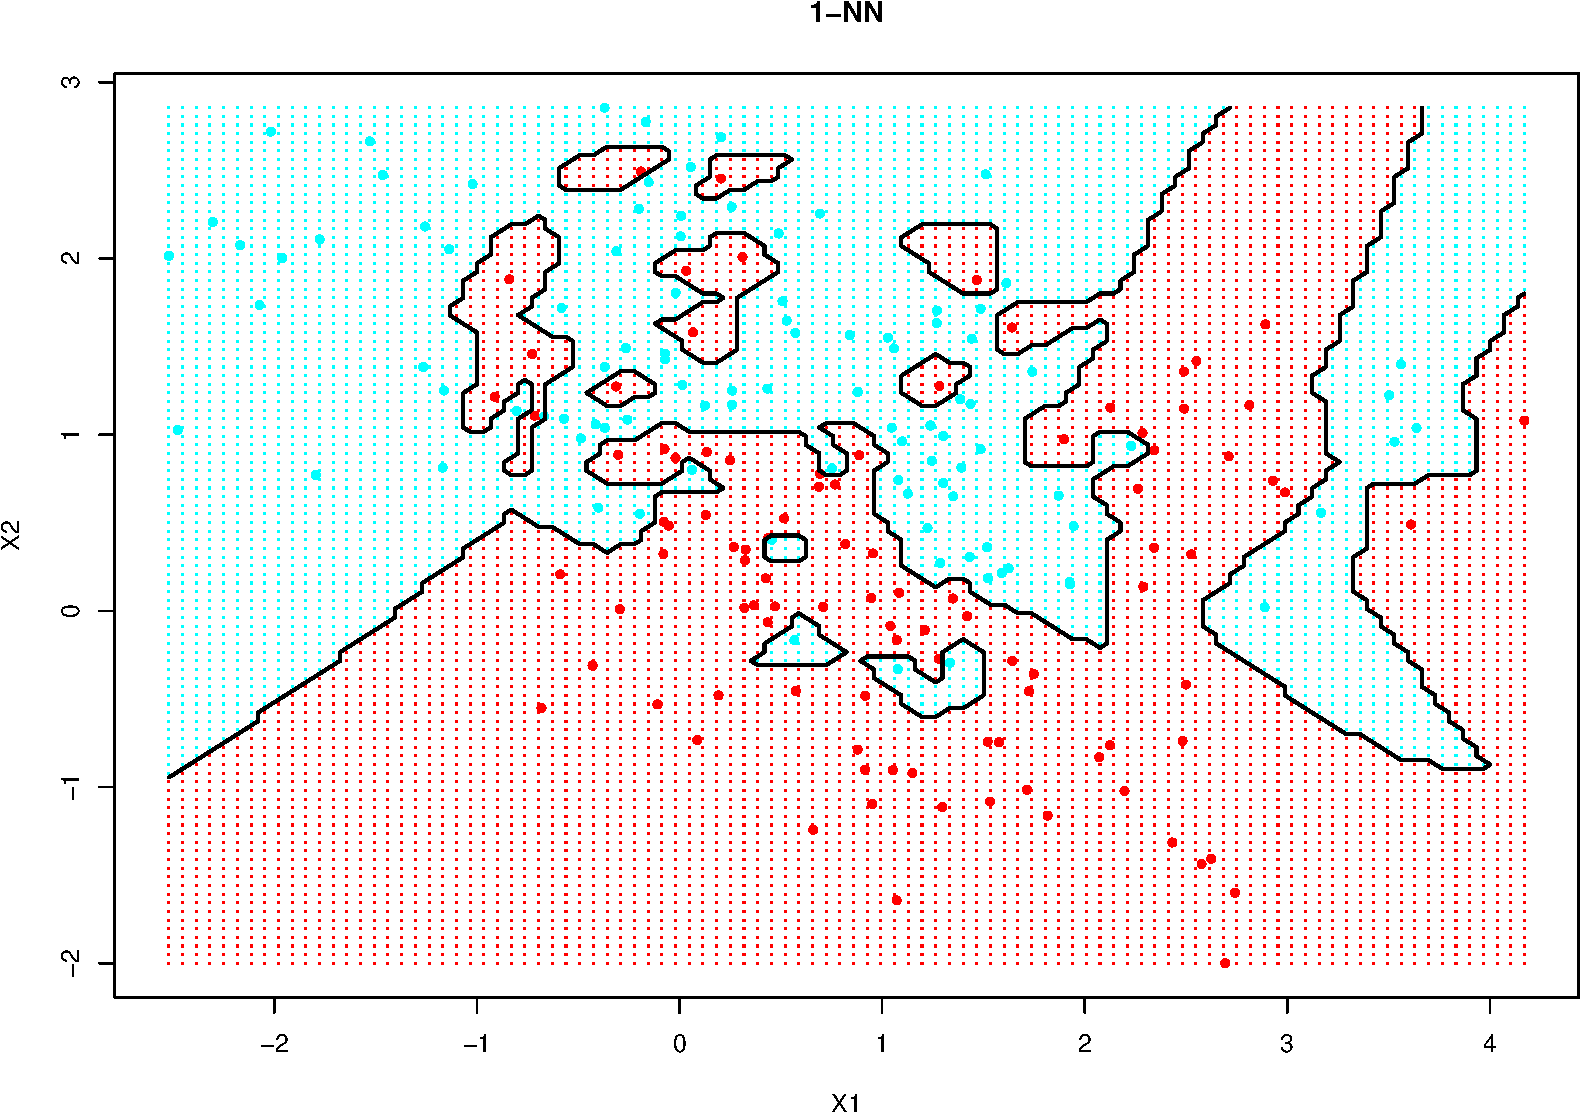
\includegraphics{EksploracjaDanych_files/figure-latex/knn1-1} 

}

\caption{Przykład klasyfikacji dla $k=1$}\label{fig:knn1}
\end{figure}

Z kolei zbyt duża liczba sąsiadów powoduje obciążenie wyników (patrz rysunek \ref{fig:knn2})

\begin{figure}

{\centering 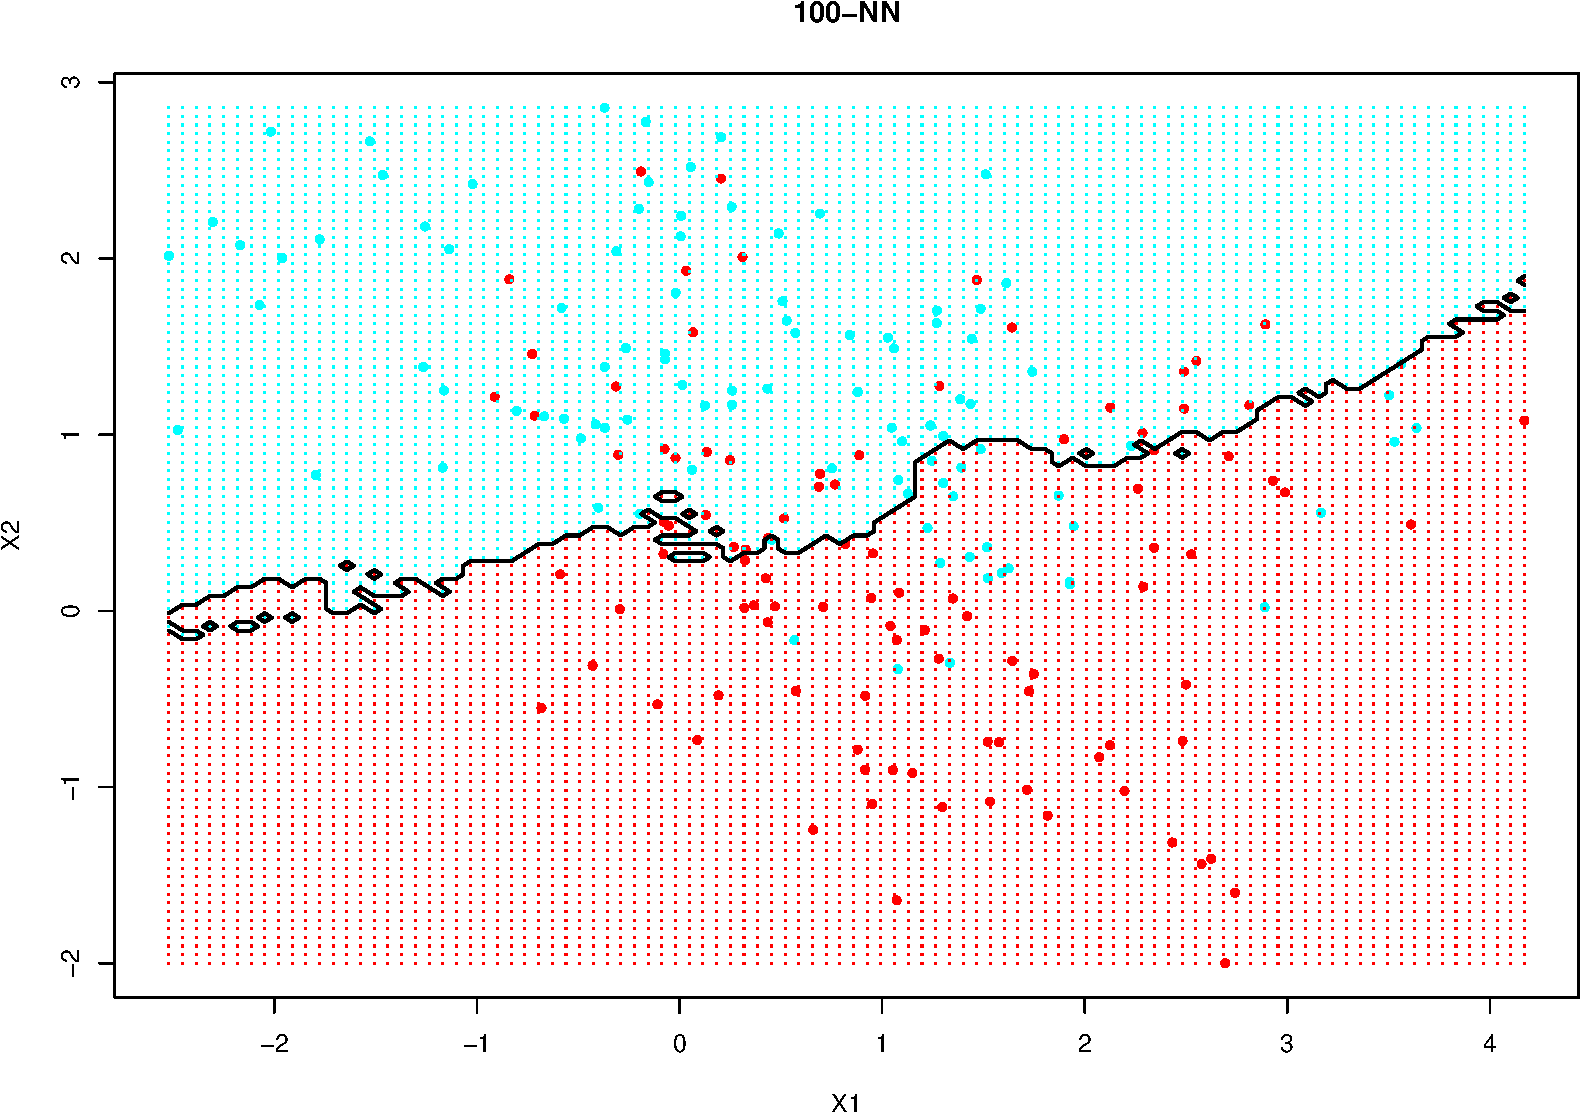
\includegraphics{EksploracjaDanych_files/figure-latex/knn2-1} 

}

\caption{Przykład zastosowania 100 sąsiadów}\label{fig:knn2}
\end{figure}

Dopiero dobór odpowiedniego \(k\) daje model o stosunkowo niskiej wariancji i obciążeniu. Najczęściej liczby \(k\) poszukujemy za pomocą próbkowania.

\begin{figure}

{\centering 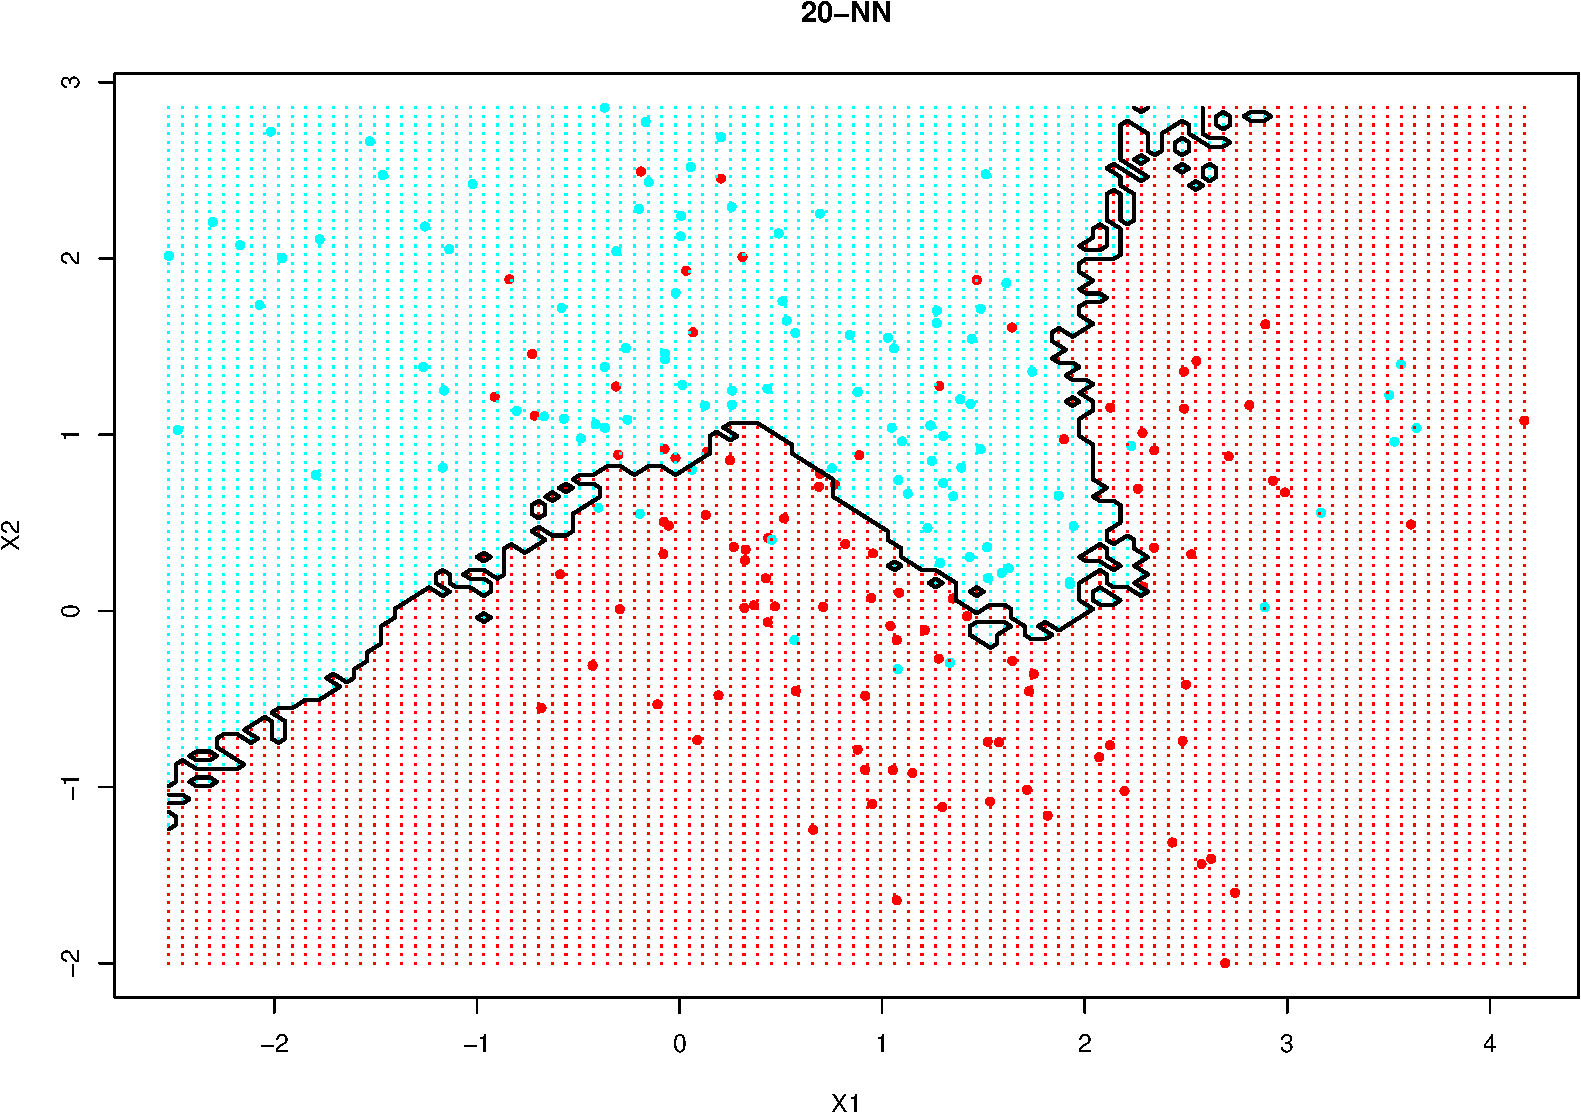
\includegraphics{EksploracjaDanych_files/figure-latex/knn3-1} 

}

\caption{Model z optymalną liczbą sąsiadów}\label{fig:knn3}
\end{figure}

\BeginKnitrBlock{example}
\protect\hypertarget{exm:knnprzklad1}{}{\label{exm:knnprzklad1} }Klasyfikację z wykorzystaniem metody \emph{kNN} przeprowadzimy na przykładzie danych zbioru \texttt{spam} pakietu \texttt{ElemStatLearn}. Metoda \emph{kNN} ma wiele implementacji R-owych ale na potrzeby przykładu wykorzystamy funkcję \texttt{knn3} pakietu \texttt{caret}.

Najpierw dokonamy oszacowania optymalnego \(k\)
\EndKnitrBlock{example}

\begin{Shaded}
\begin{Highlighting}[]
\KeywordTok{library}\NormalTok{(ElemStatLearn)}
\KeywordTok{library}\NormalTok{(tidyverse)}

\NormalTok{spam.std <-}\StringTok{ }\NormalTok{spam }\OperatorTok\StringTok{ }
\StringTok{    }\KeywordTok{mutate_if}\NormalTok{(is.numeric, scale)}
\KeywordTok{set.seed}\NormalTok{(}\DecValTok{123}\NormalTok{)}
\NormalTok{ind <-}\StringTok{ }\KeywordTok{sample}\NormalTok{(}\KeywordTok{nrow}\NormalTok{(spam), }\DataTypeTok{size =} \KeywordTok{nrow}\NormalTok{(spam)}\OperatorTok{*}\DecValTok{2}\OperatorTok{/}\DecValTok{3}\NormalTok{)}
\NormalTok{dt.ucz <-}\StringTok{ }\NormalTok{spam.std[ind,]}
\NormalTok{dt.test <-}\StringTok{ }\NormalTok{spam.std[}\OperatorTok{-}\NormalTok{ind,]}

\NormalTok{acc <-}\StringTok{ }\ControlFlowTok{function}\NormalTok{(pred, obs)\{}
\NormalTok{    tab <-}\StringTok{ }\KeywordTok{table}\NormalTok{(pred,obs)}
\NormalTok{    acc <-}\StringTok{ }\KeywordTok{sum}\NormalTok{(}\KeywordTok{diag}\NormalTok{(}\KeywordTok{prop.table}\NormalTok{(tab)))}
\NormalTok{    acc}
\NormalTok{\}}

\DecValTok{1}\OperatorTok{:}\DecValTok{40} \OperatorTok\StringTok{ }
\StringTok{    }\KeywordTok{map}\NormalTok{(}\OperatorTok{~}\KeywordTok{knn3}\NormalTok{(spam}\OperatorTok{~}\NormalTok{., }\DataTypeTok{data =}\NormalTok{ dt.ucz, }\DataTypeTok{k =}\NormalTok{ .x)) }\OperatorTok\StringTok{ }
\StringTok{    }\KeywordTok{map}\NormalTok{(}\OperatorTok{~}\KeywordTok{predict}\NormalTok{(.x, }\DataTypeTok{newdata =}\NormalTok{ dt.test, }\DataTypeTok{type =} \StringTok{"class"}\NormalTok{)) }\OperatorTok\StringTok{ }
\StringTok{    }\KeywordTok{map_dbl}\NormalTok{(}\OperatorTok{~}\KeywordTok{acc}\NormalTok{(}\DataTypeTok{pred =}\NormalTok{ .x, }\DataTypeTok{obs =}\NormalTok{ dt.test}\OperatorTok{$}\NormalTok{spam)) }\OperatorTok\StringTok{ }
\StringTok{    }\KeywordTok{tibble}\NormalTok{(}\DataTypeTok{k =} \DecValTok{1}\OperatorTok{:}\KeywordTok{length}\NormalTok{(.), }\DataTypeTok{acc=}\NormalTok{.) }\OperatorTok\StringTok{ }
\StringTok{    }\KeywordTok{ggplot}\NormalTok{(}\KeywordTok{aes}\NormalTok{(k, acc))}\OperatorTok{+}
\StringTok{     }\KeywordTok{geom_line}\NormalTok{()}
\end{Highlighting}
\end{Shaded}

\begin{figure}

{\centering 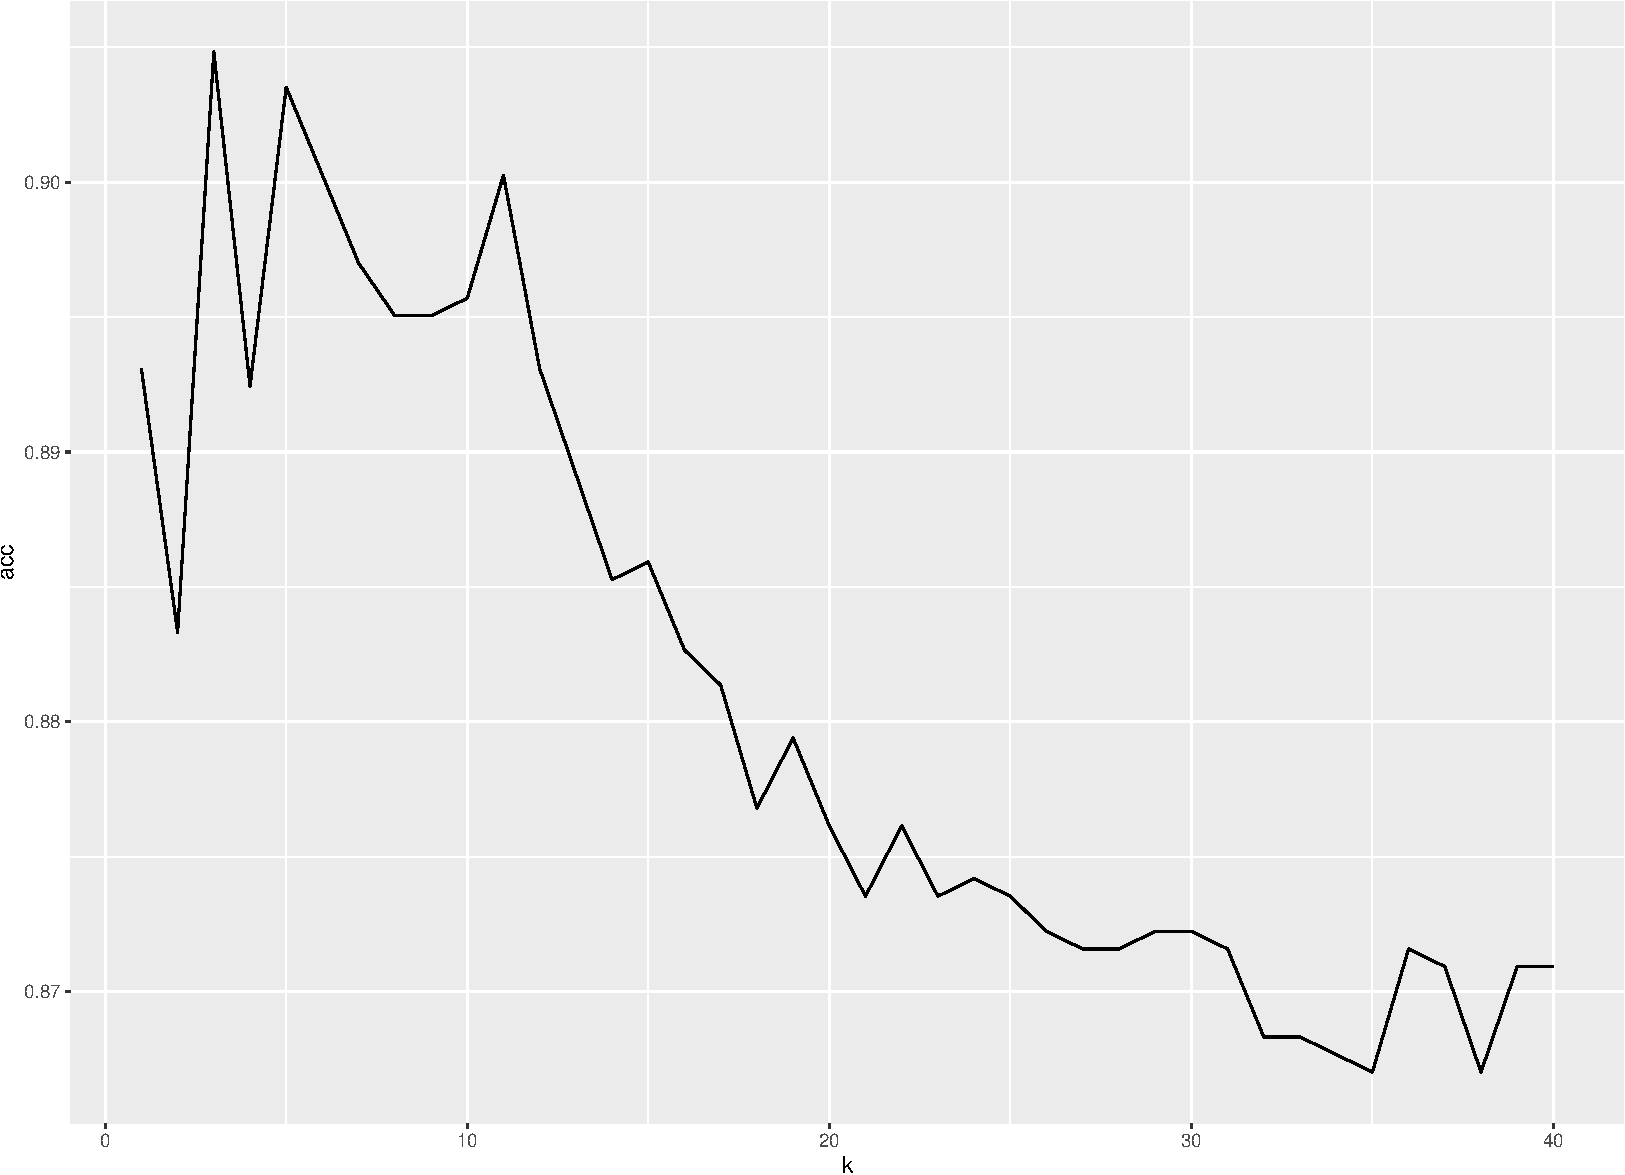
\includegraphics{EksploracjaDanych_files/figure-latex/knnrys-1} 

}

\caption{Ocena jakości dopasowania modelu dla różnej liczby sąsiadów}\label{fig:knnrys}
\end{figure}

Biorąc pod uwagę wykres \ref{fig:knnrys} można rozważać 1 lub 9 sąsiadów jako optymalne rozwiązanie, ponieważ wówczas poprawność klasyfikacji jest najwyższa. Proponuje unikać rozwiązania z 1 najbliższym sąsiadem ponieważ, będzie się ono charakteryzowało duża zmiennością. Wybór \(k=9\) wydaje się być optymalny.

\begin{Shaded}
\begin{Highlighting}[]
\NormalTok{mod.knn <-}\StringTok{ }\KeywordTok{knn3}\NormalTok{(spam}\OperatorTok{~}\NormalTok{., }\DataTypeTok{data =}\NormalTok{ dt.ucz,}
                \DataTypeTok{k =} \DecValTok{9}\NormalTok{)}
\NormalTok{mod.knn}
\end{Highlighting}
\end{Shaded}

\begin{verbatim}
## 9-nearest neighbor model
## Training set outcome distribution:
## 
## email  spam 
##  1872  1195
\end{verbatim}

Predykcji dokonujemy w ten sam sposób co w innych modelach klasyfikacyjnych

\begin{Shaded}
\begin{Highlighting}[]
\NormalTok{pred.knn.class <-}\StringTok{ }\KeywordTok{predict}\NormalTok{(mod.knn, }\DataTypeTok{newdata =}\NormalTok{ dt.test, }\DataTypeTok{type =} \StringTok{"class"}\NormalTok{)}
\KeywordTok{head}\NormalTok{(pred.knn.class)}
\end{Highlighting}
\end{Shaded}

\begin{verbatim}
## [1] spam  email email spam  spam  email
## Levels: email spam
\end{verbatim}

\begin{Shaded}
\begin{Highlighting}[]
\NormalTok{pred.knn <-}\StringTok{ }\KeywordTok{predict}\NormalTok{(mod.knn, }\DataTypeTok{newdata =}\NormalTok{ dt.test)}
\KeywordTok{head}\NormalTok{(pred.knn)}
\end{Highlighting}
\end{Shaded}

\begin{verbatim}
##          email      spam
## [1,] 0.0000000 1.0000000
## [2,] 0.6666667 0.3333333
## [3,] 0.5555556 0.4444444
## [4,] 0.2222222 0.7777778
## [5,] 0.0000000 1.0000000
## [6,] 0.8888889 0.1111111
\end{verbatim}

\begin{Shaded}
\begin{Highlighting}[]
\NormalTok{(tab <-}\StringTok{ }\KeywordTok{table}\NormalTok{(pred.knn.class, dt.test}\OperatorTok{$}\NormalTok{spam))}
\end{Highlighting}
\end{Shaded}

\begin{verbatim}
##               
## pred.knn.class email spam
##          email   863   88
##          spam     53  530
\end{verbatim}

\begin{Shaded}
\begin{Highlighting}[]
\KeywordTok{sum}\NormalTok{(}\KeywordTok{diag}\NormalTok{(}\KeywordTok{prop.table}\NormalTok{(tab)))}
\end{Highlighting}
\end{Shaded}

\begin{verbatim}
## [1] 0.9080834
\end{verbatim}

\hypertarget{uogolnione-modele-addytywne}{%
\chapter{Uogólnione modele addytywne}\label{uogolnione-modele-addytywne}}

Modele liniowe, jako techniki klasyfikacji i regresji, mają niewątpliwą zaletę - jawna postać zależności pomiędzy predyktorami i zmienną wynikową. Często w rzeczywistości tak uproszczony model nie potrafi oddać złożoności natury badanego zjawiska. Dlatego powstał pomysł aby w miejsce kombinacji liniowej predyktorów wstawić kombinację liniową ich funkcji, czyli
\begin{equation}
    \E(Y|X)=f(X) = \sum_{i=1}^M\beta_mh_m(X),
    \label{eq:row111}
\end{equation}
gdzie \(h_m:\mathbb{R}^d\to\mathbb{R}\) nazywana często funkcją bazową (ang. \emph{linear basis expansion}). Wówczas w zależności od postaci funkcji bazowej otrzymujemy modele z różnymi poziomami elastyczności:

\begin{itemize}
\tightlist
\item
  gdy \(h_m(X)=X_m,\ m=1,\ldots,M\), to otrzymujemy model liniowy;
\item
  gdy \(h_m(X)=X_j^2\) lub \(h_m(X)=X_jX_k\), to otrzymujemy struktury wielomianowe, charakteryzujące się większą elastycznością modelu;
\item
  gdy \(h_m(X)=\log X_j\) lub \(h_m(X)=\sqrt{X_j}\), to uzyskujemy nieliniowość czynników wchodzących w skład kombinacji liniowej \eqref{eq:row111};
\item
  dopuszczalne są również kawałkami liniowe funkcje postaci \(h_m(X)= I(l_m\leq X_k <u_m)\), gdzie \(I\) jest funkcją charakterystyczną (ang. \emph{indicator}) przedziału \([l_m,u_m)\).
\end{itemize}

Zbiory wszystkich funkcji bazowych definiowanych w ten sposób tworzy słownik funkcji bazowych \(\mathcal{D}\). Aby kontrolować złożoność modeli, mając do dyspozycji tak zasobny słownik, wprowadza się następujące podejścia:

\begin{itemize}
\tightlist
\item
  ogranicza się klasę dostępnych funkcji bazowych
  \begin{equation}
    f(X) = \sum_{j=1}^df_j(X_j)=\sum_{j=1}^d\sum_{m=1}^{M_j}\beta_{jm}h_{jm}(X_j),
  \end{equation}
\item
  włącza się do modelu jedynie te funkcje ze słownika \(\mathcal{D}\), które istotnie poprawiają dopasowanie modelu,
\item
  używa się metod penalizowanych, czyli dopuszcza się stosowanie wszystkich funkcji bazowych ze słownika \(\mathcal{D}\), ale współczynniki przy nich stojące są ograniczane.
\end{itemize}

\hypertarget{przypadek-jednowymiarowy}{%
\section{Przypadek jednowymiarowy}\label{przypadek-jednowymiarowy}}

Dla uproszczenia rozważań przyjmiemy, że \(X\) jest jednowymiarowe.

\begin{figure}

{\centering 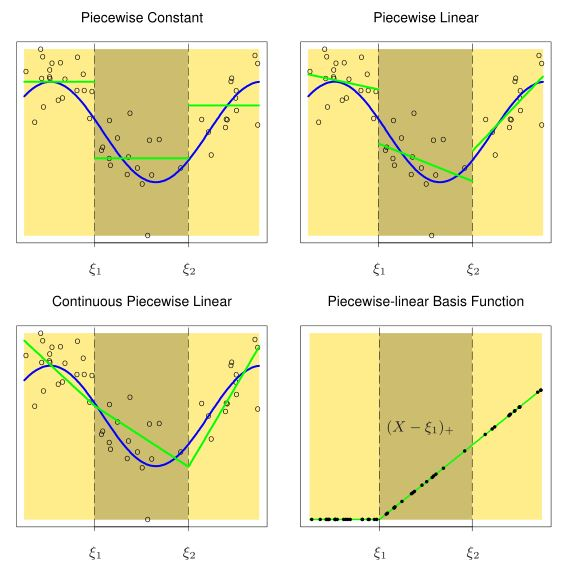
\includegraphics{images/spline1} 

}

\caption{Przykładowe zastosowanie kilku rodzajów funkcji bazowych. Wykres w lewym górnym rogu powstał ze stałych na przedziałach, wykres w górnym prawym rogu powstał z liniowych funkcji bazowych na przedzialach, w lewym dolnym rogu model powstał również z liniowych funkcji bazowych na przedzialach ale z założeniem ciągłości, a prawym dolnym rogu powstał z zastosowania funcji bazowej $\max(X-\xi_1,0)$}\label{fig:spline1}
\end{figure}

\begin{figure}

{\centering 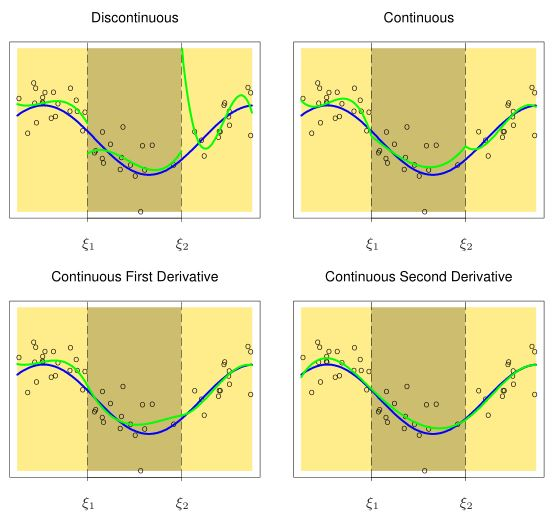
\includegraphics{images/spline2} 

}

\caption{Kolejne wykresy przedstawiają coraz bardziej gładkie modele będące efektem dodawania wielomianów trzeciego stopnia na przedziałach. Na każdym kolejnym modelu mymuszone zostały silniejsze założenia dotyczące gładkości}\label{fig:spline2}
\end{figure}

Przykładowo sześcienny splajn\footnote{czyli funkcja łączona} dla dwóch punków węzłowych składa się z następujących funkcji bazowych

\begin{gather}
    h_1(X)=1,\quad h_3(X)=X^2,\quad h_5(X)=(X-\xi_1)_+^3\\
    h_2(X)=X,\quad h_4(X)=X^3,\quad h_6(X)=(X-\xi_2)_+^3.
\end{gather}

Zachowanie wielomianów poza punktami węzłowymi jest czasami bardzo dziwne. Zdarza się, że charakteryzują się tam dużą zmiennością. Dlatego wprowadza się takie splajny aby w obszarach brzegowych zachowywały się przewidywalnie.
Naturalny splajn sześcienny zakłada liniowość modelu poza węzłami brzegowymi. Dla \(K\) węzłów naturalny splajn sześcienny składa się z następujących funkcji bazowych

\begin{gather}
    N_1(X)=1,\quad N_2(X)=X,\quad N_{k+2}(X)=d_k(X)-d_{K-1}(X),
\end{gather}
gdzie \(d_k(X)=\frac{(X-\xi_k)^3_+-(X-\xi_K)^3_+}{\xi_K-\xi_k}.\)

Estymacji parametrów modelu dokonujemy metodą najmniejszych kwadratów, minimalizując
\begin{equation}
    RSS(f,\lambda) = \sum_{i=1}^N(y_i-f(x_i))^2+\lambda\int(f''(t))^2dt,
\end{equation}
gdzie \(\lambda\) jest parametrem wygładzania. Pierwsze wyrażenie po prawej stronie to ocena dopasowania, a drugie to kara za krzywoliniowość.
Dla naturalnego splajna
\begin{equation}
    f(x)=\sum_{j=1}^NN_j(x)\beta_j
\end{equation}
minimalizujemy
\begin{equation}
    RSS(\beta, \lambda)=(\boldsymbol y -\boldsymbol N\beta)'(\boldsymbol y-\boldsymbol N\beta)+\lambda\beta'\boldsymbol \Omega \beta,
\end{equation}
gdzie \(\{\boldsymbol N\}_{ij}= N_j(x_i)\) i \(\{\boldsymbol \Omega\}_{jk}=\int N''_j(t)N''_k(t)dt\). Rozwiązaniem zaganienia minimalizacji \(RSS(\beta,\lambda)\) jest
\begin{equation}
    \hat{\beta}=((\boldsymbol N'\boldsymbol N)+\lambda\boldsymbol \Omega)^{-1}\boldsymbol N'\boldsymbol y.
\end{equation}

\hypertarget{przypadek-wielowymiarowy}{%
\section{Przypadek wielowymiarowy}\label{przypadek-wielowymiarowy}}

W przypadku gdy \(X\in \mathbb{R}^d\) poszukujemy takiej \(d\)-wymiarowej regresji \(f(x)\), która będzie minimalizowała wyrażenie
\begin{equation}
    \min_f\sum_{i=1}^N(y_i-f(x_i))^2+\lambda J(f),
\end{equation}
gdzie \(J\) jest odpowiednią funkcją wyrażającą krzywoliniowość modelu. Dla \(X\in \mathbb{R}^2\) przyjmuje postać
\begin{equation}
    J(f)=\iint_{\mathbb{R}^2}\left[\left(\frac{\partial^2 f(x)}{\partial^2 x_1}\right)^2+2\left(\frac{\partial^2 f(x)}{\partial x_1\partial x_2}\right)^2+
    \left(\frac{\partial^2 f(x)}{\partial^2 x_2}\right)^2\right]dx_1dx_2.
\end{equation}
Rozwiązanie przyjmuje postać
\begin{equation}
    f(x) = \beta_0+\beta'x+\sum_{i=1}^N \alpha_ih_i(x),
\end{equation}
gdzie \(h_i(x)=||x-x_j||^2\log||x-x_j||\).

\hypertarget{uogolnione-modele-addytywne-1}{%
\section{Uogólnione modele addytywne}\label{uogolnione-modele-addytywne-1}}

Przez uogólnione modele addytywne (ang. \emph{Generalized Additive Models}) rozumiemy klasę modeli, które poprzez funkcję łączącą, opisują warunkową wartość zmiennej wynikowej w następujący sposób
\begin{equation}
    g(\E(Y|X))=g(\mu(X))=\alpha+f_1(X_1)+\dots+f_d(X_d),
\end{equation}
gdzie \(g\) jest funkcją łączącą. Najczęściej stosowanymi funkcjami łączącymi są:

\begin{itemize}
\tightlist
\item
  \(g(\mu)=\mu\) - stosowana w modelach, gdy zmienna wynikowa ma rozkład normalny;
\item
  \(g(\mu)=\logit\mu\) - stosowana, gdy zmienna wynikowa ma rozkład dwumianowy;
\item
  \(g(\mu)=\probit\mu\) - stosowana również w przypadku gdy zmienna ma rozkład dwumianowy, a \(\Phi^{-1}\) oznacza odwrotność dystrybuanty standaryzowanego rozkładu normalnego;
\item
  \(g(\mu)=\log\mu\) - stosowana, gdy zmienna wynikowa jest zmienną typu zliczeniowego (rozkład Poissona).
\end{itemize}

\hypertarget{algorytm-uczenia-modelu-gam}{%
\subsection{Algorytm uczenia modelu GAM}\label{algorytm-uczenia-modelu-gam}}

Algorytm uczenia wstecznego (ang. \emph{backfitting}) przebiega wg następujących kroków:

\begin{enumerate}
\def\labelenumi{\arabic{enumi}.}
\tightlist
\item
  Ustalamy wstępne oszacowania na \(\alpha=\bar{y}\) i \(\hat{f}_j=0\).
\item
  Dla \(j=1,\ldots,d,1,\ldots,d,1,\ldots\) powtarzamy szacowanie
  \begin{align}
   \hat{f}_j\leftarrow &\mathcal{S}_j\left[(y_i-\hat{\alpha}-\sum_{k\neq j}\hat{f}_k(x_{ik}))^N_1\right],\\
   \hat{f}_j\leftarrow &\hat{f}_j-\frac{1}{N}\sum_{i=1}^N\hat{f}_j(x_{ij})
  \end{align}
  dopóki \(\hat{f}_j\) osiągnie zbieżność. Funkcja \(\mathcal{S}_j\left[(y_i-\hat{\alpha}-\sum_{k\neq j}\hat{f}_k(x_{ik}))^N_1\right]\) jest jednowymiarowym sześciennym splajnem o \(N\) węzłach. W jej miejsce można przyjąć również inne funkcje, takie jak: jednowymiarowe lokalne regresje wielomianowe (ang. \emph{LOESS - locally estimated scatterplot smoothing}), regresje liniowe, wielomianowe.
\end{enumerate}

\BeginKnitrBlock{example}
\protect\hypertarget{exm:gam}{}{\label{exm:gam} }Dla zilustrowania zasady działania uogólnionych modeli addytywnych przeprowadzimy analizę stężenia ozonu (\(O_3\)) w zależności od wybranych parametrów meteorologicznych. Do zbudowania modelu GAM wykorzystamy funkcję \texttt{gam} pakietu \texttt{mgcv} (Wood \protect\hyperlink{ref-R-mgcv}{2003}).
\EndKnitrBlock{example}

\begin{Shaded}
\begin{Highlighting}[]
\KeywordTok{library}\NormalTok{(faraway)}
\KeywordTok{head}\NormalTok{(ozone)}
\end{Highlighting}
\end{Shaded}

\begin{verbatim}
##   O3   vh wind humidity temp  ibh dpg ibt vis doy
## 1  3 5710    4       28   40 2693 -25  87 250  33
## 2  5 5700    3       37   45  590 -24 128 100  34
## 3  5 5760    3       51   54 1450  25 139  60  35
## 4  6 5720    4       69   35 1568  15 121  60  36
## 5  4 5790    6       19   45 2631 -33 123 100  37
## 6  4 5790    3       25   55  554 -28 182 250  38
\end{verbatim}

\begin{Shaded}
\begin{Highlighting}[]
\KeywordTok{library}\NormalTok{(mgcv)}
\NormalTok{mod.gam <-}\StringTok{ }\KeywordTok{gam}\NormalTok{(O3}\OperatorTok{~}\KeywordTok{s}\NormalTok{(temp, }\DataTypeTok{bs =} \StringTok{"cr"}\NormalTok{, }\DataTypeTok{m =} \DecValTok{2}\NormalTok{)}\OperatorTok{+}\KeywordTok{s}\NormalTok{(ibh)}\OperatorTok{+}\KeywordTok{s}\NormalTok{(ibt), }\DataTypeTok{data =}\NormalTok{ ozone)}
\KeywordTok{summary}\NormalTok{(mod.gam)}
\end{Highlighting}
\end{Shaded}

\begin{verbatim}
## 
## Family: gaussian 
## Link function: identity 
## 
## Formula:
## O3 ~ s(temp, bs = "cr", m = 2) + s(ibh) + s(ibt)
## 
## Parametric coefficients:
##             Estimate Std. Error t value Pr(>|t|)    
## (Intercept)  11.7758     0.2382   49.44   <2e-16 ***
## ---
## Signif. codes:  0 '***' 0.001 '**' 0.01 '*' 0.05 '.' 0.1 ' ' 1
## 
## Approximate significance of smooth terms:
##           edf Ref.df      F  p-value    
## s(temp) 3.357  4.216 20.758 5.99e-16 ***
## s(ibh)  4.171  5.072  7.344 1.37e-06 ***
## s(ibt)  2.111  2.729  1.403    0.213    
## ---
## Signif. codes:  0 '***' 0.001 '**' 0.01 '*' 0.05 '.' 0.1 ' ' 1
## 
## R-sq.(adj) =  0.708   Deviance explained = 71.7%
## GCV = 19.348  Scale est. = 18.724    n = 330
\end{verbatim}

W powyższym modelu użyto splajnów jako funkcji \(f_i\). W przypadku zmiennej \texttt{temp} był to sześcienny splajn z regularyzacją w postaci ciągłości drugiej pochodnej, a pozostałe są prostymi splajnami. Dopasowanie modelu sięga 71.7\% a wartość uogólnionego sprawdzianu krzyżowego 19.35.

Poniższy wykres pokazuje rodzaje transformacji użyte przy dopasowaniu modelu.

\begin{Shaded}
\begin{Highlighting}[]
\KeywordTok{par}\NormalTok{(}\DataTypeTok{mfrow =} \KeywordTok{c}\NormalTok{(}\DecValTok{1}\NormalTok{,}\DecValTok{3}\NormalTok{))}
\KeywordTok{plot}\NormalTok{(mod.gam, }\DataTypeTok{shade =}\NormalTok{ T, }\DataTypeTok{residuals =}\NormalTok{ T)}
\end{Highlighting}
\end{Shaded}

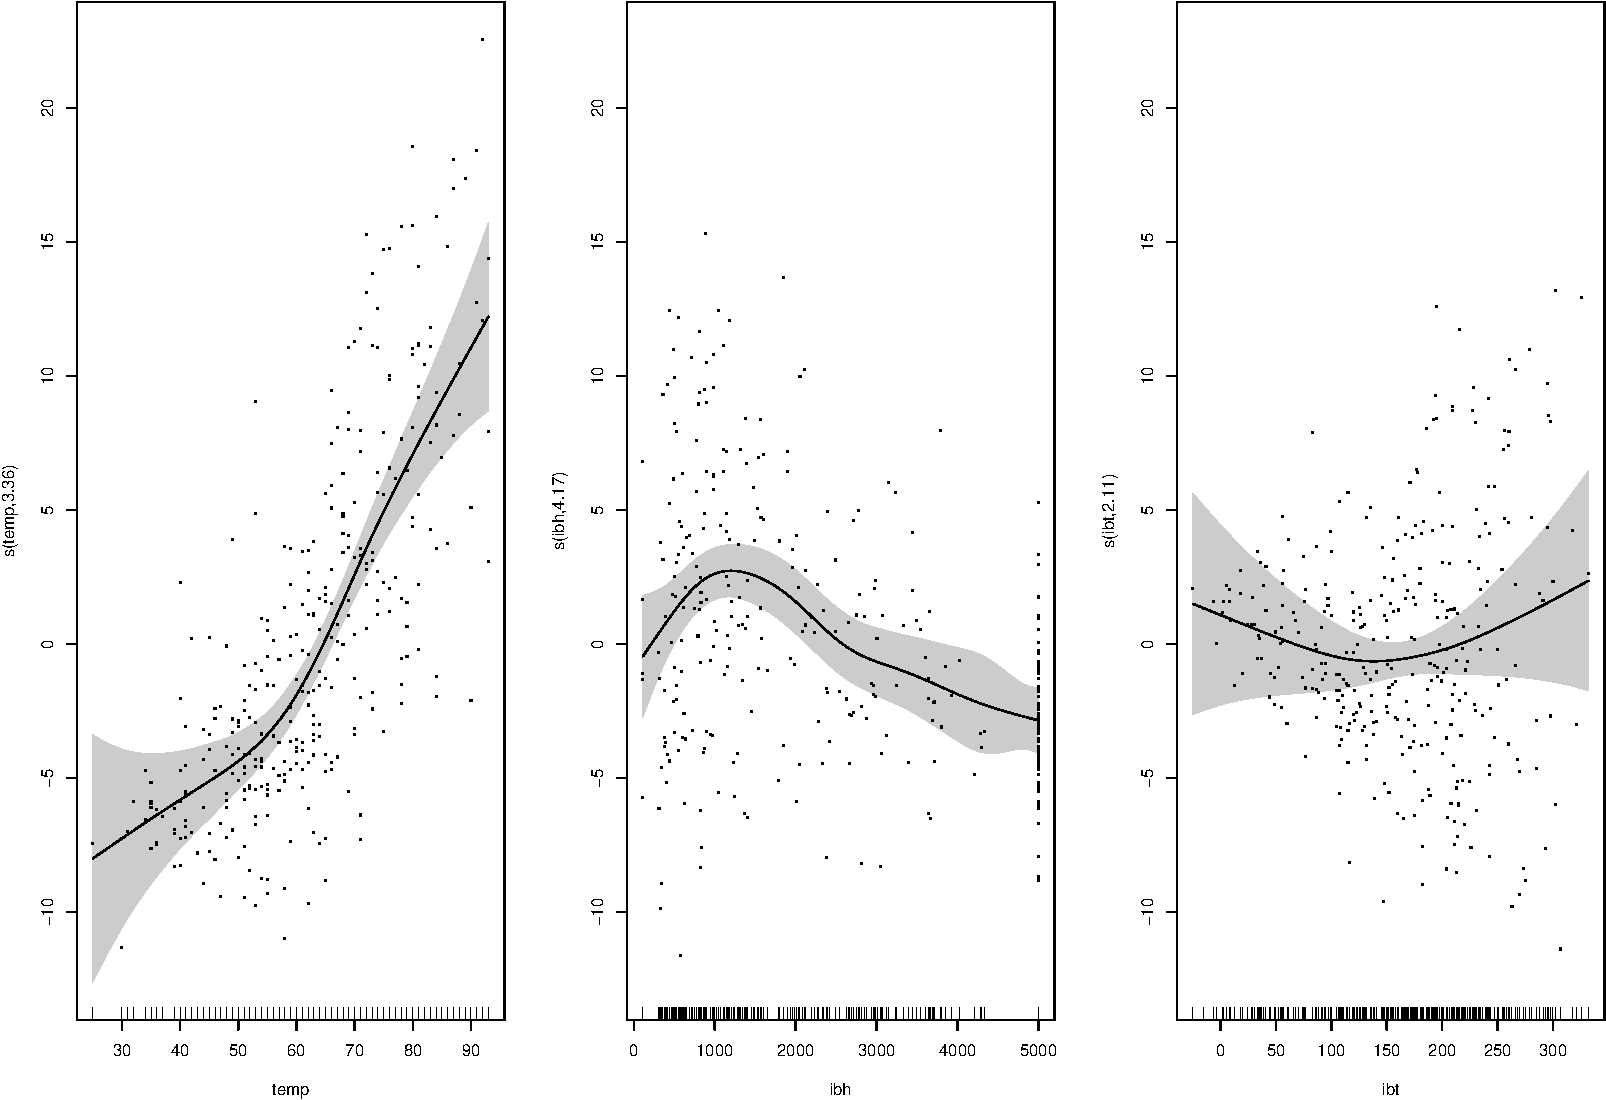
\includegraphics{EksploracjaDanych_files/figure-latex/unnamed-chunk-85-1.pdf}

\begin{Shaded}
\begin{Highlighting}[]
\KeywordTok{par}\NormalTok{(}\DataTypeTok{mfrow=}\KeywordTok{c}\NormalTok{(}\DecValTok{1}\NormalTok{,}\DecValTok{1}\NormalTok{))}
\end{Highlighting}
\end{Shaded}

\hypertarget{refs}{}
\leavevmode\hypertarget{ref-R-rmarkdown}{}%
Allaire, JJ, Yihui Xie, Jonathan McPherson, Javier Luraschi, Kevin Ushey, Aron Atkins, Hadley Wickham, Joe Cheng, Winston Chang, and Richard Iannone. 2018. \emph{Rmarkdown: Dynamic Documents for R}. \url{https://CRAN.R-project.org/package=rmarkdown}.

\leavevmode\hypertarget{ref-breiman1996}{}%
Breiman, Leo. 1996. ``Bagging Predictors.'' \emph{Machine Learning} 24 (2): 123--40. \url{https://doi.org/10.1007/BF00058655}.

\leavevmode\hypertarget{ref-breiman1998}{}%
---------. 1998. ``Arcing Classifier (with Discussion and a Rejoinder by the Author).'' \emph{Ann. Statist.} 26 (3). The Institute of Mathematical Statistics: 801--49. \url{https://doi.org/10.1214/aos/1024691079}.

\leavevmode\hypertarget{ref-R-rio}{}%
Chan, Chung-hong, and Thomas J. Leeper. 2018. \emph{Rio: A Swiss-Army Knife for Data I/O}. \url{https://CRAN.R-project.org/package=rio}.

\leavevmode\hypertarget{ref-R-janitor}{}%
Firke, Sam. 2018. \emph{Janitor: Simple Tools for Examining and Cleaning Dirty Data}. \url{https://CRAN.R-project.org/package=janitor}.

\leavevmode\hypertarget{ref-fisher1936}{}%
Fisher, R. A. 1936. ``The Use of Multiple Measurements in Taxonomic Problems.'' \emph{Annals of Eugenics} 7 (2): 179--88. \url{https://doi.org/10.1111/j.1469-1809.1936.tb02137.x}.

\leavevmode\hypertarget{ref-friedman1989}{}%
Friedman, Jerome H. 1989. ``Regularized Discriminant Analysis.'' \emph{Journal of the American Statistical Association} 84 (405): 165--75. \url{https://doi.org/10.2307/2289860}.

\leavevmode\hypertarget{ref-R-gbm}{}%
Greenwell, Brandon, Bradley Boehmke, Jay Cunningham, and GBM Developers. 2019. \emph{Gbm: Generalized Boosted Regression Models}. \url{https://CRAN.R-project.org/package=gbm}.

\leavevmode\hypertarget{ref-ho1995}{}%
Ho, Tin Kam. 1995. ``Random Decision Forests.'' In \emph{Proceedings of 3rd International Conference on Document Analysis and Recognition}, 1:278--82. IEEE.

\leavevmode\hypertarget{ref-R-Rweka}{}%
Hornik, Kurt, Christian Buchta, and Achim Zeileis. 2009. ``Open-Source Machine Learning: R Meets Weka.'' \emph{Computational Statistics} 24 (2): 225--32. \url{https://doi.org/10.1007/s00180-008-0119-7}.

\leavevmode\hypertarget{ref-R-party}{}%
Hothorn, Torsten, Kurt Hornik, and Achim Zeileis. 2006. ``Unbiased Recursive Partitioning: A Conditional Inference Framework.'' \emph{Journal of Computational and Graphical Statistics} 15 (3). Taylor \& Francis: 651--74. \url{https://doi.org/10.1198/106186006X133933}.

\leavevmode\hypertarget{ref-R-partykit}{}%
Hothorn, Torsten, and Achim Zeileis. 2015. ``Partykit: A Modular Toolkit for Recursive Partytioning in R.'' \emph{Journal of Machine Learning Research} 16: 3905--9. \url{http://jmlr.org/papers/v16/hothorn15a.html}.

\leavevmode\hypertarget{ref-kuhn}{}%
Jed Wing, Max Kuhn. Contributions from, Steve Weston, Andre Williams, Chris Keefer, Allan Engelhardt, Tony Cooper, Zachary Mayer, et al. 2018. \emph{Caret: Classification and Regression Training}. \url{https://CRAN.R-project.org/package=caret}.

\leavevmode\hypertarget{ref-kavakiotis2017}{}%
Kavakiotis, Ioannis, Olga Tsave, Athanasios Salifoglou, Nicos Maglaveras, Ioannis Vlahavas, and Ioanna Chouvarda. 2017. ``Machine Learning and Data Mining Methods in Diabetes Research.'' \emph{Computational and Structural Biotechnology Journal} 15: 104--16.

\leavevmode\hypertarget{ref-kearns1989}{}%
Kearns, M., and L. G. Valiant. 1989. ``Crytographic Limitations on Learning Boolean Formulae and Finite Automata.'' \emph{Annual ACM Symposium on Theory of Computing}, 433. \url{http://search.ebscohost.com/login.aspx?direct=true\&db=edb\&AN=73725380\&lang=pl\&site=eds-live\&scope=site}.

\leavevmode\hypertarget{ref-R-C50}{}%
Kuhn, Max, and Ross Quinlan. 2018. \emph{C50: C5.0 Decision Trees and Rule-Based Models}. \url{https://CRAN.R-project.org/package=C50}.

\leavevmode\hypertarget{ref-R-las}{}%
Liaw, Andy, and Matthew Wiener. 2002. ``Classification and Regression by randomForest.'' \emph{R News} 2 (3): 18--22. \url{https://CRAN.R-project.org/doc/Rnews/}.

\leavevmode\hypertarget{ref-R-e1071}{}%
Meyer, David, Evgenia Dimitriadou, Kurt Hornik, Andreas Weingessel, and Friedrich Leisch. 2019. \emph{E1071: Misc Functions of the Department of Statistics, Probability Theory Group (Formerly: E1071), Tu Wien}. \url{https://CRAN.R-project.org/package=e1071}.

\leavevmode\hypertarget{ref-R-ipred}{}%
Peters, Andrea, and Torsten Hothorn. 2018. \emph{Ipred: Improved Predictors}. \url{https://CRAN.R-project.org/package=ipred}.

\leavevmode\hypertarget{ref-quinlan1993}{}%
Quinlan, J Ross. 1993. \emph{C4. 5: Programs for Machine Learning}. Morgan Kaufmann.

\leavevmode\hypertarget{ref-R-base}{}%
R Core Team. 2018. \emph{R: A Language and Environment for Statistical Computing}. Vienna, Austria: R Foundation for Statistical Computing. \url{https://www.R-project.org/}.

\leavevmode\hypertarget{ref-schapire1990}{}%
Schapire, Robert E. 1990. ``The Strength of Weak Learnability.'' \emph{Machine Learning} 5 (2): 197--227. \url{https://doi.org/10.1007/BF00116037}.

\leavevmode\hypertarget{ref-R-CHAID}{}%
Team, The FoRt Student Project. 2015. \emph{CHAID: CHi-Squared Automated Interaction Detection}.

\leavevmode\hypertarget{ref-R-VIM}{}%
Templ, Matthias, Alexander Kowarik, Andreas Alfons, and Bernd Prantner. 2019. \emph{VIM: Visualization and Imputation of Missing Values}. \url{https://CRAN.R-project.org/package=VIM}.

\leavevmode\hypertarget{ref-R-rpart}{}%
Therneau, Terry, and Beth Atkinson. 2018. \emph{Rpart: Recursive Partitioning and Regression Trees}. \url{https://CRAN.R-project.org/package=rpart}.

\leavevmode\hypertarget{ref-R-DMwR}{}%
Torgo, Luis. 2013. \emph{DMwR: Functions and Data for "Data Mining with R"}. \url{https://CRAN.R-project.org/package=DMwR}.

\leavevmode\hypertarget{ref-R-mda}{}%
Trevor Hastie, S original by, Robert Tibshirani. Original R port by Friedrich Leisch, Kurt Hornik, and Brian D. Ripley. 2017. \emph{Mda: Mixture and Flexible Discriminant Analysis}. \url{https://CRAN.R-project.org/package=mda}.

\leavevmode\hypertarget{ref-R-mice}{}%
van Buuren, Stef, and Karin Groothuis-Oudshoorn. 2018. \emph{Mice: Multivariate Imputation by Chained Equations}. \url{https://CRAN.R-project.org/package=mice}.

\leavevmode\hypertarget{ref-R-MASS}{}%
Venables, W. N., and B. D. Ripley. 2002. \emph{Modern Applied Statistics with S}. Fourth. New York: Springer. \url{http://www.stats.ox.ac.uk/pub/MASS4}.

\leavevmode\hypertarget{ref-R-klaR}{}%
Weihs, Claus, Uwe Ligges, Karsten Luebke, and Nils Raabe. 2005. ``KlaR Analyzing German Business Cycles.'' In \emph{Data Analysis and Decision Support}, edited by D. Baier, R. Decker, and L. Schmidt-Thieme, 335--43. Berlin: Springer-Verlag.

\leavevmode\hypertarget{ref-welch1939}{}%
Welch, B. L. 1939. ``Note on Discriminant Functions.'' \emph{Biometrika} 31 (1/2): 218--20. \url{https://doi.org/10.2307/2334985}.

\leavevmode\hypertarget{ref-R-mgcv}{}%
Wood, S. N. 2003. ``Thin-Plate Regression Splines.'' \emph{Journal of the Royal Statistical Society (B)} 65 (1): 95--114.

\leavevmode\hypertarget{ref-R-bookdown}{}%
Xie, Yihui. 2018a. \emph{Bookdown: Authoring Books and Technical Documents with R Markdown}. \url{https://CRAN.R-project.org/package=bookdown}.

\leavevmode\hypertarget{ref-R-knitr}{}%
---------. 2018b. \emph{Knitr: A General-Purpose Package for Dynamic Report Generation in R}. \url{https://CRAN.R-project.org/package=knitr}.


\end{document}
